\documentclass[16pt,a4paper,openany,twoside]{book}

\usepackage[pdftex]{graphicx}
\usepackage{caption}
\usepackage{subcaption}
\usepackage[top=1in, bottom=1in, left=1.5in, right=1in]{geometry}
\usepackage{setspace}
\usepackage{tocbibind}
\usepackage{lineno}
\usepackage{definitions}
\usepackage{amssymb}
\usepackage{rotating}
\usepackage{multirow}
\usepackage[nomain,acronym,toc,nopostdot,nonumberlist]{glossaries}
\usepackage[pdftex,pdftitle={Dissertation},pdfauthor={John Garland Wood}]{hyperref}
\usepackage{chngpage} 

\author{John Garland Wood}

\makeglossaries
\newacronym{sm}{SM}{Standard Model}
\newacronym{bsm}{BSM}{Beyond the Standard Model}

\newacronym{cern}{CERN}{European Center for Nuclear Research}
\newacronym{lhc}{LHC}{Large Hadron Collider}
\newacronym{atlas}{ATLAS}{A Toroidal LHC Apparatus}
\newacronym{cms}{CMS}{Compact Muon Solenoid}
\newacronym{ecal}{ECAL}{Electromagnetic Calorimeter}
\newacronym{hcal}{HCAL}{Hadronic Calorimeter}

\newacronym{qft}{QFT}{Quantum Field Theory}
\newacronym{qed}{QED}{Quantum Electrodynamics}
\newacronym{qcd}{QCD}{Quantum Chromodynamics}
\newacronym{lo}{LO}{Leading Order}
\newacronym{nlo}{NLO}{Next to Leading Order}
\newacronym{isr}{ISR}{Initial State Radiation}
\newacronym{fsr}{FSR}{Final State Radiation}

\newacronym{mva}{MVA}{Multi-Variate Analysis}
\newacronym{ann}{ANN}{Artificial Nueral Network}
\newacronym{mlp}{MLP}{Multi-Layer Perceptron}
\newacronym{cfmlp}{CFMLP}{Cleinman-Freidman Multi-Layer Perceptron}
\newacronym{bdt}{BDT}{Boosted Decision Tree}

\newacronym{jhep}{JHEP}{Journal of High Energy Physics}

\global\def\@title{The Search for Higgs Boson Production in Association with a Top-Quark Pair in $pp$ Collisions at $\sqrt{s}$ = 8 TeV in the Lepton Plus Jets Final State}
\title{\@title}

\begin{document}
%%\setlength{\parindent}{1cm}

\frontmatter
\begin{titlepage}
  \centering
  \doublespacing
  
  \vspace*{0.5in}
  \textbf{\Large \@title}\\[0.75in]
  Brian Patrick Francis\\
  Charlottesville, VA\\[0.5in]
  B.S., The University of Massachusetts Amherst, 2009\\[1.5in]
  A Dissertation presented to the Graduate Faculty\\
  of the Unversity of Virginia in Candidacy for the Degree of\\
  Doctor of Philosophy\\[0.5in]
  Department of Physics\\[0.5in]
  University of Virginia\\
  May, 2015\\

\end{titlepage}
\doublespacing
\begin{center}

\textbf{\Large Abstract}\\[0.25in]

\end{center}

\par The most important goal of the \acrfull{lhc} is to elucidate the mechanism of electroweak symmetry breaking.  The \acrfull{sm} Higgs boson is thought to be a prime candidate for this.  The newly discovered boson announced on July 4th, 2012, with a mass of ${\sim}125$~\GeVcc, has so far been shown to be consistent with a \acrshort{sm} Higgs.  However, the final confirmation of this new particle as the \acrshort{sm} Higgs depends on subsequent measurements of all of its properties.  The observation of this new particle in association with top-quark pairs would allow the couplings of this particle to top and bottom quarks to be directly measured. ~\ttH, with Higgs decaying to~\bbbar~is an excellent channel to explore due to the dominant branching ratio of Higgs to~\bbbar~and  the kinematic handle the~\ttbar~system offers on the event.  However, it presents a plethora of difficult challenges due to a low signal to background ratio and uncertainties on kinematically similar \acrshort{sm} backgrounds.  This work discusses the search for Higgs boson production in association with a top-quark pair in~\pp~collisions at $\sqrt{s}$ = 8~\TeV, collected by the \acrfull{cms} experiment at the \acrshort{lhc}.  The search has been performed and published in two stages.  The first analysis used the first 5.1~\fbinv, and was followed up by the second analysis with the full 2012 dataset, using a total integrated luminosity of 19.5~\fbinv     


\def\signrule{\vskip 0.75in\hbox{\vrule width 3.5in height 0.4pt \hskip 0.3in
 \vrule width 2in height 0.4pt}}

\newpage

\vbox{
  \thispagestyle{empty}
  \begin{singlespace}
    \hbox{We approve the dissertation of John Garland Wood.}
    \vskip 0.35in 
    \hbox{\null\hskip 3.9in Date of Signature}
    \signrule
    \raggedright\begin{tabular}{l}Supervisor: Prof. Christopher Neu\end{tabular}\par
    \vskip -0.2in
    \signrule
    \raggedright\begin{tabular}{l}Committee Member: Prof. Hank Thacker\end{tabular}\par
    \vskip -0.2in
    \signrule
    \raggedright\begin{tabular}{l}Committee Member: Prof. Edward Murphy\end{tabular}\par
    \vskip -0.2in
    \signrule
    \raggedright\begin{tabular}{l}Committee Member: Prof. Bradley Cox\end{tabular}\par
    %\raggedright\begin{tabular}{l}Committee Member: Prof. Bradley Cox\end{tabular}\par
    \vskip 0.75in
    \signrule
    %\raggedright\begin{tabular}{l}PhD Committee Chair: Prof. Bradley Cox\end{tabular}\par
    \raggedright\begin{tabular}{l}PhD Committee Chair: Prof. Craig Group\end{tabular}\par
    
  \end{singlespace}
} 
\newpage

\tableofcontents
\listoffigures
\listoftables
%\clearpage

\mainmatter
\linenumbers
\chapter{Introduction}
\label{introduction}

\begin{figure}
    \centering
    \begin{subfigure}[b]{0.3\textwidth}
        \label{fig:qft_lo_ee_scattering}
        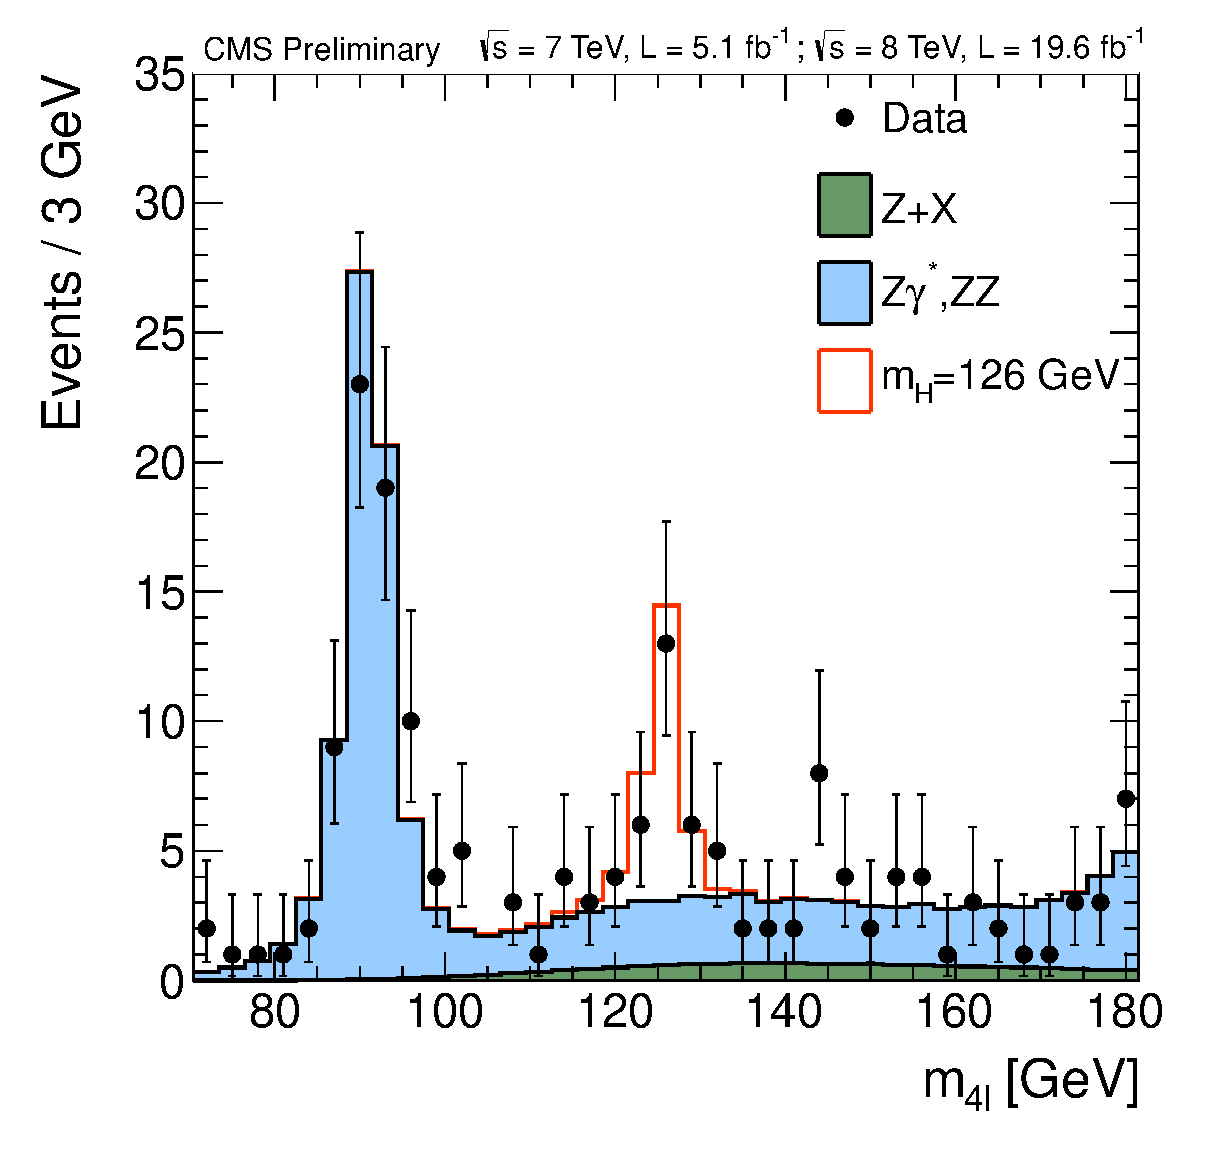
\includegraphics[width=\textwidth]{Figures/Experimental_Results/CmsHZZ4lMass.eps}
        \caption{CMS results for the $H\rightarrow~ZZ$ channel}
      \end{subfigure}
      ~ %add desired spacing between images, e. g. ~, \quad, \qquad, \hfill etc.
      % (or a blank line to force the subfigure onto a new line)
      \begin{subfigure}[b]{0.3\textwidth}
          \label{fig:qft_nlo_ee_scattering}
          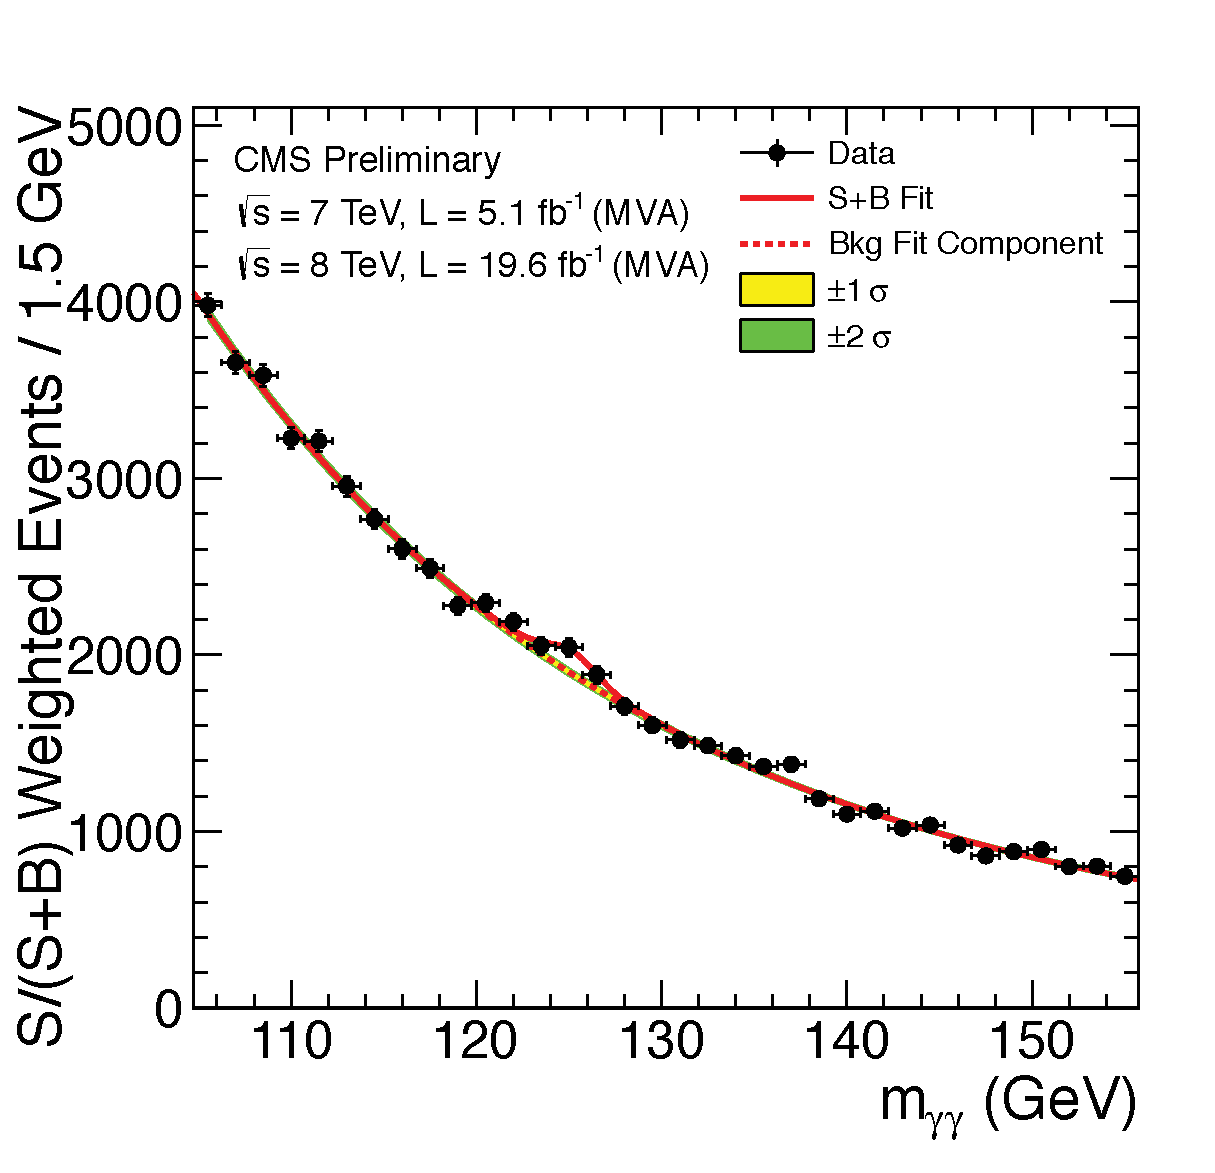
\includegraphics[width=\textwidth]{Figures/Experimental_Results/CmsHggMassMVAMoriond13.eps}
          \caption{CMS results for the $H\rightarrow\gamma\gamma$ channel}
      \end{subfigure}
      \caption{The CMS experiment has observed a new boson at m$\sim$125\GeVcc} \label{fig:cms_hZZ_hgg_results}
\end{figure}

\par On July 4th, 2012, the \acrfull{cms} and \acrfull{atlas} experiments announced the discovery of a new boson of mass $\sim~125$~\GeVcc~\cite{CMS:2012discovery}~\cite{ATLAS:2012discovery}.  The particle has been shown to be increasingly consistent with the description of the boson predicted by the Higgs mechanism of the \acrshort{sm}, as measurements on its mass, width, and quantum numbers are completed.  However, there are several properties of this new boson, which remain to be tested.  Figure \ref{fig:cms_hZZ_hgg_results} shows a consistent mass peak betwen the $H\rightarrow~ZZ$ and $H\rightarrow\gamma\gamma$ channels at the \acrshort{cms} experiment.  

\par The Yukawaka coupling of the Higgs boson to the top-quark in the \acrshort{sm} is the largest coupling among the fundamental particles and is well 
predicted - thus offering an excellent test of the nature of the coupling of the Higgs to fermions, as well as a potential probe into pysics \acrfull{bsm} that would alter this value from the \acrshort{sm} prediction.  The production of the Higgs boson in association with top-quark pairs is the best production mode at the \acrshort{lhc} that offers direct access to the top-Higgs coupling.  The dominant production mode of Higgs at the \acrshort{lhc}, gluon-gluon fusion, involves a triangle loop of strongly-coupled fermions, which includes all of the other quarks, as well as the potential for \acrshort{bsm} particles.  

\par ~\ttH~production also has the ability to constrain some extensions of the \acrshort{sm} that would not modify the Higgs branching fractions enough to be seen 
within current experiemental precision.  Such models include Little Higgs models, models with extra dimensions, top-color models, and compositie Higgs models that introduce a vector-like top partner, a $t'$, that can decay to $tH$, $bW$, or $tZ$ states.  Both $t't'$ and $t't$ production would produce a~\ttH~final state, or one that is indistinguishable from it ($tHbW$).  Upper limits on~\ttH~production would also provide limits on the previously described models, which would be complementary to existing direct searches for $t'$ particles, which attempt to reconstruct the $t'$ resonance.  

\par The~\ttH~channel has a rich set of possible final states.  Each top-quark will decay to a $b$-quark and a $W$ boson.  The $W$ boson will subsequently decay to two quarks, or a lepton and a neutrino.  These decays are classified as either hadronic, semi-leptonic, or di-leptonic for zero, one, or both $t$ quarks decaying leptonically 
respectively.  The Higgs may to decay to $b$-quark, $W$, $Z$, $\tau$, or $\gamma$ pairs.  In fact, this is one of the only production modes at the \acrshort{lhc} which 
has access to every Higgs decay mode, as other production mechanisms are swamped by large backgrounds preventing measurements of all Higgs decay types.  

\par The search is performed with the \acrshort{cms} experiment, a modern, general purpose particle detector capable of reconstructing and identifying hadronic jets, photons, electrons, muons, and tau leptons.  The hermetic design, and it's high precision and efficiency in reconstrucing and tracking every particle in a $pp$ collision, also makes it suitable for reconstructing missing transverse energy from the calculated momentum imbalance of all of the measured particles in the event.  This missing transverse energy is often the signature of a neutrino, which is the only \acrshort{sm} particle capable of escaping detection.  The detector uses a 3.8 T axial magnetic field, produced by the solenoid it is named after, to bend charged particles as they travel through the detector.  The measured curvature of their tracks allows the momentum of the particles to be calculated with to a high precision.  Tracks are formed and particles are reconstructed by a combination of sub-detector systems which work together to form the final final reconstructed image of each particle in the collision.  

\begin{figure}[h]
   \centering
  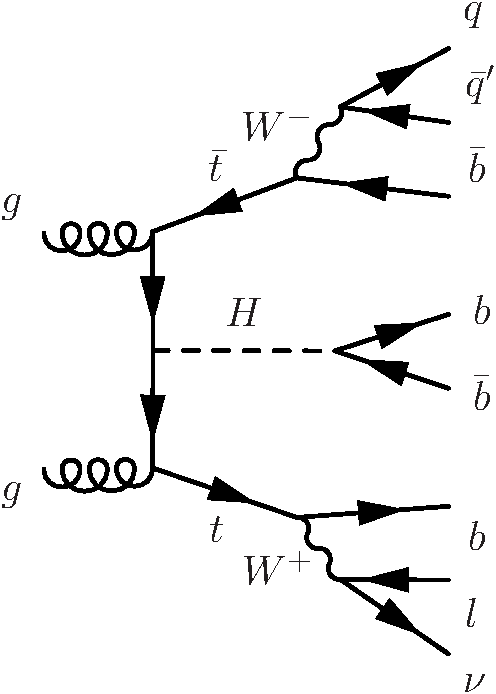
\includegraphics[width=0.5\textwidth]{Figures/Feynman_Diagrams/higgs_production__tth_semileptonic.pdf}
  \caption{A Feynman diagram of the~\ttH~process, with Higgs$\rightarrow$$b\bar{b}$, and the $t\bar{t}$-system decaying semi-leptonically} \label{fd:ttH_semiLep}
\end{figure}

\par This thesis will focus on a semi-leptonic decay of the top-quarks, with the Higgs decaying to a $b$-quark pair.  Figure \ref{fd:ttH_semiLep} is Feynman diagrm of the~\ttH~process.  The largest background to this process is top-quark pair production with extra jets originating from \acrfull{isr} or \acrfull{fsr} radiation,~\ttjets.  The irreducible background is formed by top-quark pairs, where a gluon is radiated and decays to $b$-quark pairs,~\ttbb.  In addition to the large backgrounds, the high jet multiplicity in the~\ttH~final state gives rise to a combinatorics problem in associating each jet with its role in the~\ttH~system.  This inevitably leads to misidentifying which jets are the decay product of the Higgs, and thus additionally smears out the resolution on the mass of the Higgs.  Due to the similarity of the~\ttbb~background and the combinatorics issue, no single variable is suitable for signal extraction.  A \acrfull{mva} technique is used in an attempt to isolate the~\ttH~signal from the~\ttjets background.  The \acrshort{mva} provides a one-dimensional discriminant based on several input variables related to the kinematics of the event.  This discrimant is then used to perform signal extraction and set upper-limits on~\ttH~ production.  The results of two searches will be presented.  The first result used the first 5.1~\fbinv of the 2012 dataset, with center of mass energy of 8~\TeV, and was published in the \acrfull{jhep}, May 2013.  The second result was update with the full 19.4~\fbinv 8~\TeV dataset, and was published in \acrshort{jhep}, Spetember 2014.   

\chapter{Theoretical Background}
\label{theoretical_background}

\par The \acrfull{sm} of particle physics represents the sum of
knowledge of the fundamental particles and their interactions with
each other.  It is a \acrfull{qft} that represents the interactions of each of the
fundamental forces through the symmetry of a mathematical object
known as a Lie group.  It is the theory that dictates the rate that
the~\ttH~process is produced, as well as the kinematics of every
particle involved.  As such, its predictions are critical for modeling
the charateristic signature of the~\ttH~signal in the \acrshort{cms}
detector, as well as the background processes, like~\ttbb~which leave
a kinematically similar final state signature.     


\section{An Overview of Quantum Field Theory}
\label{qft_overview}

\par \acrfull{qft} was developed out of the need for a
relativistic description of quantum mechanics.  Since the Einstein
relation $E=mc^{2}$ allows for the creation of particle-antiparticle
pairs, the single-particle description used in non-relativistic quantum
mechanics, fails describe this phenomenom~\cite{Peskin_Schroeder}.
This additionally fails when considering that Heisenberg's uncertainty
relation, $\Delta~E\cdot~\Delta~t = \hbar$, allows for an arbitrary
number of intermediate, virtual particles to be created.  By
quantizing a field representing a certain type of particle,
multiparticle states are naturally described as discreet excitations
of that field.  

% Lorentz invariance reveals a relationship between matter/antimatter
\par Lorentz invariance, and the need to preserve causality, also define a
fundamental relationship between matter and antimatter.  The
propagation of a particle across a space-like interval is treated
equivalently to the an anti-particle propagating in the opposite
direction~\cite{Peskin_Schroeder}.  This is done so that the net
probability amplitude for the particles to have an effect on a 
measurment occuring accross a space-like interval cancel each other,
thus preserving cuasality.  This cancellation requirement additionally
implies that the particle and anti-particle have the same mass, with
opposite quantum numbers such as spin or electric charge.   

% Accounting for spin 
\par The Lorentz transformations for a scalar field are different than
for a field with internal degrees of freedom, such as spin.  A
rotation on a vector field, will affect both its location, as well as
it's orentation~\cite{Peskin_Schroeder}.  This means the Lorentz
invariant equation of motion descirbing a scalar field will have a
different form than equations of motion for a field with spin.  The
most relevant equations describe the particles of \acrshort{sm}, which
contain spins of 0, 1/2, and 1.  They are described by the
Klein-Gordan, Dirac, and Proca equations respectively. \\

\noindent Klein-Gordon equation, for scalar (spin 0) fields 
\begin{equation}\label{eq:klein_gordon_eom}
(\partial^{2} + m^{2})\phi = 0  
\end{equation} 

\noindent Dirac equation, for spinor (spin 1/2) fields 
\begin{equation}\label{eq:dirac_eom}
(i\gamma^{\mu}\partial_{\mu} - m)\psi = 0 
\end{equation} 

\noindent Proca equation, for vector (spin 1) fields
\begin{equation}\label{eq:proca_eom}
\partial_{\mu}(\partial^{\mu}A^{\nu} - \partial^{\nu}A^{\mu}) + m^{2}A^{\nu}
= 0 
\end{equation} 

% From the free fields to interactions
\par With these equations, one can build a theory of free particles.
The Lagrangian formulation is the most appropriate since all
expressions are explicitly Lorentz invariant~\cite{Peskin_Schroeder}.
The Lagrangians for the Klein-Gordon, Dirac, and Proca equations are
given as: \\

\noindent Klein-Gordon Lagrangian, for real and complex scalar fields
\begin{equation}\label{eq:klein_gordon_lagrangian}
\begin{aligned}
& \mathcal{L} = \partial_{\mu}\partial^{\mu}\phi^{2} - \frac{1}{2}m^{2}\phi^{2}  \\
& \mathcal{L} = (\partial_{\mu}\phi)^{\ast}(\partial^{\mu}\phi) - m^{2}(\phi)^{\ast}(\phi) 
\end{aligned}
\end{equation}

\noindent Dirac Lagrangian, for spinor fields
\begin{equation}\label{eq:dirac_lagrangian}
\mathcal{L} = i\bar{\psi}\gamma^{\mu}\partial_{\mu}\psi - m\bar{\psi}\psi 
\end{equation}

\noindent Proca Lagrangian, for vector fields
\begin{equation}\label{eq:proca_lagrangian}
\mathcal{L} = -\frac{1}{4}F_{\mu\nu}F^{\mu\nu} + m^{2}A^{\nu}A_{\mu} 
\end{equation}

\noindent where $F_{\mu\nu}$, is the field strength tensor, defined as
$F_{\mu\nu} = \partial_{\mu}A_{\nu} - \partial{\nu}A_{\mu}$

\par Interactions are generated by coupling multiple fields together in a
single term, such as $ieA_{\mu}\bar{\psi}\psi$ and treating it as a
perturbation to the free field theory.  This implies every interaction
between particles is carried out by a virtual mediating particle.  When two
electrons scatter off one another, they are really exchanging a
virtual photon, the mediator of the electromagnetic force.  The
$W^{\pm} and Z$ bosons mediate the weak force, while the $gluons$
mediate the strong force.  

\begin{equation}\label{eq:lagrangian_free_interacting}
\mathcal{L} = \mathcal{L}_{Free} + \mathcal{L}_{Interacting}
\end{equation}

% Feynmann rules provide the method of calculating physical observables
\par In order to calculate the probability and dynamics of two
particles interacting with one another, an integral, constrained by
energy and momentum conservation, over the phase space of outgoing
particles and the scattering amplitude, $mathcal{M}$, is evaluated.
The scattering amplitude is calculated by using the propagtor (Green's
function of the free particle theory) for the incoming, mediating, and
outgoing particles, with an appropriate wieghting function, or vertex
factor, for each point the particles interact in the scattering
process, and then integrating over the momentum of the mediating
particle.  Richard Feynmann developed a set of rules for the writing
down the propagators and vertex factors directly from the Lagrangian,
and easily computing the scattering amplitude.  He also introduced an
elegant pictographic notation useful for visualizing particle
interactions, known as Feynmann diagrams. 

\begin{figure}
    \centering
    \begin{subfigure}[h]{0.45\textwidth}
        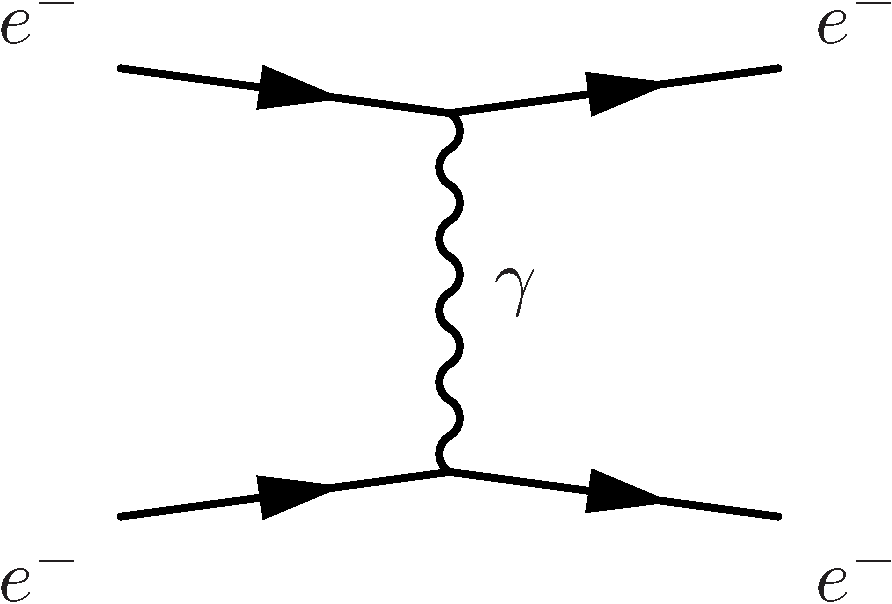
\includegraphics[width=\textwidth]{Figures/Feynman_Diagrams/qft_ex__lo_diagram__coulomb_scattering.pdf}
        \caption{A LO Feynman diagram }\label{fig:qft_lo_ee_scattering}
      \end{subfigure}
      ~ %add desired spacing between images, e. g. ~, \quad, \qquad, \hfill etc.
      % (or a blank line to force the subfigure onto a new line)
      \begin{subfigure}[h]{0.45\textwidth}
          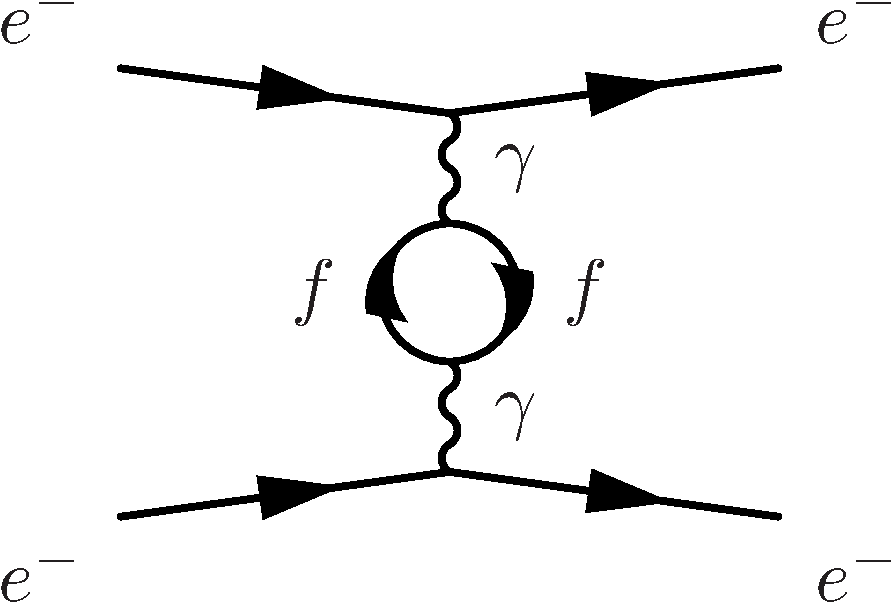
\includegraphics[width=\textwidth]{Figures/Feynman_Diagrams/qft_ex__nlo_diagram__coulomb_scattering.pdf}
          \caption{A NLO Feynman diagram}\label{fig:qft_nlo_ee_scattering}
      \end{subfigure}
      \caption{Leading and Next to Leading Order Feynman diagrams
        for the coulomb scattering process} \label{fig:feynman_diagrams_ee_scattering}
\end{figure}

\par With these tools, one can calculate the probability amplitudes of
a given process occuring to \acrfull{lo} without any
difficulties.  However, when calculations in \acrfull{nlo} are
performed, and loop diagrams of virtual particles are considered, the
probability amplitudes associated with a given process diverge to
infinity.  This occurs when one integrates over all of the 
possible momentum allowed by intermediate, loops of virtual particles,
which due to Heisenberg's uncertainty principle, are allowed to take
on any value of momentum.  Figure
\ref{fig:feynman_diagrams_ee_scattering} shows an example of a
\acrshort{lo} and \acrshort{nlo} process.

\begin{figure}[h]
  \centering
  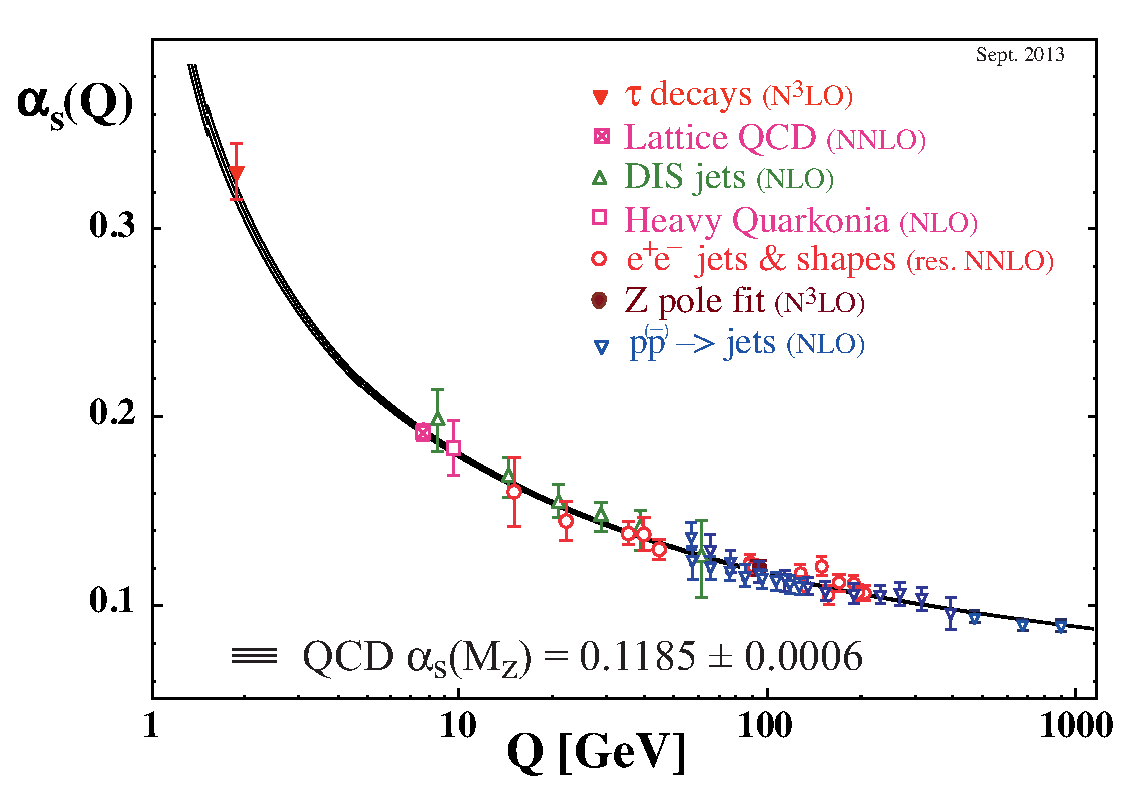
\includegraphics[width=0.5\textwidth]{Figures/Experimental_Results/asq-2013.eps}
  \caption{The global average of $\alpha_{s}$, the QCD coupling
    constant.}\label{fig:globalAvgAlphaS}
\end{figure}

\par The systematic removal of divergences from a theory is called
renormalization.  The divergences are absorbed into the
definitions of the free parameters of the theory, making the parameters a function of
the energy scale the process occurs at, instead of a constant.  This
allows for the calculations of fundamental processes to completed,
as long as the energy scale of the interaction is known.  A modern
interpretation of renormalization was provided by Kenneth
Wilson~\cite{th:Wilson_renormalization1}~\cite{th:Wilson_renormalization2}.
Instead of seeing the effects of high momentum calculations after
moving to \acrshort{nlo} in perturbation theory, one uses an effective Lagrangian,
computed by integrating out shells of momentum beginning at the energy
cutoff of the theory, where the \acrshort{nlo} effects begin the
dominate.  The dimensions of integration are then rescaled and the
result of evaluating the integral over the momentum shell is absorbed
into the definition of free parameters.  The processes is iterated
until the energy scale of the interaction is reached.  The functional 
dependence of the parameters is then  directly present in the resulting
effective Lagrangian, instead of appearing suddenly when accounting
for the one-loop contributions at \acrshort{nlo}.  Regardless of how
strange this procedure seem, the running of the coupling constant as a
function of interaction engergy has been validated experimentally time
and time and again, as shown in Figure \ref{fig:globalAvgAlphaS}~\cite{Bethke_WorldAvgAlphaS_QCD}.


\section{Abelian Gauge Theories of Particle Interactions}
\label{abelian_gauge_theory_overview}

\par In 1930, Herman Weyl introduced the idea that the interactions
between fields can be generated by requiring them to be invariant
under guage tansformations of a local symmetry~\cite{Weyl}.  For
electromagnetism, the local symmetry is that of the Lie group,
$U(1)$.  It is an abelian group, which has the property that the
generators of the group symmetry commutes with themselves. 
The $U(1)$ symmetry is invariant under phase rotations.  By requiring
local guage invariance, the Lagrangian must be unchanged under the 

\begin{equation}\label{eq:u1_psi_transformation}
\psi(x) \rightarrow e^{i\alpha(x)}\psi(x).
\end{equation}

Consider the Lagrangian for a free spin 1/2 particle: 

\begin{equation}\label{eq:dirac_lagrangian}
\mathcal{L} = \bar{\psi}(i\gamma^{\mu}\partial_{\mu} - m)\psi
\end{equation}

\noindent The first term in the Lagrangian, involving the derivative,
acts on $\alpha(x)$, creating a new term in the Lagrangian, breaking
its invariance under the local phase transformation.  

\begin{equation}\label{eq:u1_lagrangian_transformation}
\mathcal{L}\rightarrow\mathcal{L} -
(\partial_{\mu}\alpha)\bar{\psi}\gamma^{\mu}\psi
\end{equation}

\noindent Thus, a new term must be added to the orginial Lagrangian to cancel
out the term arising from the local phase transformation.  This is
achieved by defining the covariant derivative:

\begin{equation}\label{eq:covariant_derivative_em}
D_{\mu} = \partial_{\mu} + ieA_{\mu}
\end{equation} 

\noindent where $A_{\mu}$ is a new vector field that transforms as follows:

\begin{equation}\label{eq:u1_Afield_transformation}
A_{\mu}(x) \rightarrow A_{\mu}(x) - \frac{1}{e}\partial_{\mu}\alpha(x)
\end{equation}

\noindent The covariant derivative thus transforms like

\begin{equation}\label{eq:u1_covariant_derivative_transformation}
\begin{aligned}
D_{\mu}\psi(x) & \rightarrow [ \partial_{\mu} + ie(A_{\mu} -
\frac{1}{e}\partial_{\mu}\alpha) ]e^{i\alpha(x)}D_{\mu}\psi(x) \\
& = e^{i\alpha(x)}[ \partial_{\mu} + ie(A_{\mu} -
\frac{1}{e}\partial_{\mu}\alpha + \frac{1}{e}\partial_{\mu}\alpha) ]D_{\mu}\psi(x) \\
 & = e^{i\alpha(x)}(\partial_{\mu} + ieA_{\mu})\psi(x) \\
 & = e^{i\alpha(x)}D_{\mu}\psi(x)
\end{aligned}
\end{equation}

\noindent This covariant derivative transforms in the smae way that $\psi(x)$
does, and the new locally guage invariant Lagrangian becomes

\begin{equation}\label{eq:u1_invariant_lagrangian}
\begin{aligned}
\mathcal{L} & = \bar{\psi}(i\gamma^{\mu}D_{\mu} - m)\psi - \frac{1}{4}F^{\mu\nu}F_{\mu\nu} \\
& = i\bar{\psi}\gamma\partial_{\mu}\psi -
\bar{\psi}\gamma^{\mu}\psi~A_{mu} - m\bar{\psi}\psi -
\frac{1}{4}F^{\mu\nu}F_{\mu\nu} 
\end{aligned}
\end{equation}

\noindent where

\begin{equation}\label{eq:u1_field_strength_tensor}
F^{\mu\nu} = (\partial^{\mu}A^{\nu} - \partial^{\nu}A^{\mu})
\end{equation}

\noindent and $\frac{1}{4}F^{\mu\nu}F_{\mu\nu} $ is the kinetic energy
term of the Proca equation for the new vector field.

\par This new Lagrangian is identical to the \acrshort{qed}
Lagrangian, excpet it was derived beginning with a free dirac theory
and requiring the field to be locally guage invariant under $U(1)$
transformations.  This necessitated the introduction of a new vector
field, $A_{\mu}$, as well as an interaction term with it.  This
implies that the electromagnetic force can be represented by the
requirement of local $U(1)$ symmetry on a free Dirac particle.  

\par It should be noted, that if the photon had mass, an additional
term from the Proca equation would have to be added to the Lagrangian,
$m^{2}A_{\mu}A^{\mu}$.  This term complicates the picture since it is
not invariant under local phase transformations, and cannot be
compensated for through a different choice of $A_{\mu}$.  This implies
that the bosons of a guage theory must be massless in order to
preserve local guage invariance.  


\section{Non-Abelian Gauge Theories of Particle Interactions}
\label{non_abelian_gauge_theory_overview}
\par In 1954, Yang and Mills worked to extend this idea to symmetries
of different guage groups~\cite{th:Yang_Mills}.  Their most imortant
accomplishment was developing this procedure for non-abelian groups.
These are groups, where the transformation does not involve a simple
variable $\alpha(x)$, but rather an entire matrix of dimension n$>$2.
These matrices do no commute with each other, and their work developed
the procedure for applying local guage invariance described above to
the more complex, higher dimensional symmetries, such as $SU(2)$ and
$SU(3)$.  Consider the case of $SU(2)$ symmetry.  The theory is
appropriate for describing the dynamics of two fermion fields,
represented as a doublet:

\begin{equation}\label{eq:yang_mills_fermion_doublet}
\psi = \binom{\psi_{1}(x)}{\psi_{2}(x)}
\end{equation}

\noindent this will transform under the $SU(2)$ transformation as a
two-component spinor:

\begin{equation}\label{eq:yang_mills_fermion_transformaiton}
\psi \rightarrow \text{ exp}\langle~i\alpha^{i}\frac{\sigma_{i}}{2}\rangle\psi
\end{equation} 

\noindent where $\sigma^{i}$ are the Pauli matrices:

\begin{equation}\label{eq:pauli_matrices}
\sigma^{1} = 
  \begin{pmatrix}
    0  &  1 \\
    1  &  0
  \end{pmatrix}
\text{   ,    }
\sigma^{2} = 
  \begin{pmatrix}
    0  & -i \\
    i  &  0
  \end{pmatrix}
\text{   ,   }
\sigma^{3} = 
  \begin{pmatrix}
    1  &   0 \\
    0  & -1
  \end{pmatrix}
\end{equation}

\noindent and have the commutation relation defined by:

\begin{equation}\label{eq:pauli_matrices_commutator}
[\frac{\sigma^{i}}{2}\text{, }\frac{\sigma^{j}}{2}] =
i\epsilon^{ijk}\frac{\sigma^{k}}{2}
\end{equation}

\par Similar to the case of the $U(1)$ Abelian symmetry, in order to form
a lagrangian that is locally guage invariant, three vector fields,
$A_{\mu}^{i}$, $i=1,2,3$, are introduced, and coupled to $\psi$
through the covariant derivative:

\begin{equation}\label{eq:yang_mills_covariant_derivative}
D_{\mu} = (\partial_{\mu} - igA_{\mu}^{i}\frac{\sigma^{i}}{2})
\end{equation}

\noindent to ensure that the derivative covaries with the
transformation, the fields, $A_{\mu}^{i}$ will transform like:

\begin{equation}\label{eq:yang_mills_vector_field_transformation}
A_{\mu}^{i}\frac{\sigma^{i}}{2} \rightarrow
A_{\mu}^{i}\frac{\sigma^{i}}{2} +
\frac{1}{g}(\partial_{\mu}\alpha^{i})\frac{\sigma
^{i}}{2} +
i[\frac{\alpha^{i}\sigma{i}}{2}\text{,
}A_{\mu}^{i}\frac{\sigma^{i}}{2}]
\end{equation}

\noindent The third term, which was absent from the abelian form of
the transformation, is necessary to account for the non-commutation of
the pauli matrices.  This non-communtation also changes the form of
the field strength tensor, $F_{\mu\nu}^{i}$:

\begin{equation}\label{eq:yang_mills_field_strength_tensor}
F_{\mu\nu}^{i} = \partial_{\mu}A_{\nu}^{i} - \partial_{\nu}A_{\mu}^{i} + g\epsilon^{ijk}A_{\mu}^{j}A_{\nu}^{k}
\end{equation}

\noindent The entire $SU(2)$ invariant Lagrangian can then be written
as:

\begin{equation}\label{eq:yang_mills_invariant_lagrangian}
\begin{aligned}
\mathcal{L}_{Yang-Mills} & = -\frac{1}{4}F_{\mu\nu}^{i}F^{i\mu\nu} +
\bar{\psi}(i\gamma^{\mu}D_{\mu})\psi \\
 & = -\frac{1}{4}F_{\mu\nu}^{i}F^{i\mu\nu} +
\bar{\psi}(i\gamma^{\mu}\partial_{\mu} -
igA_{\mu}^{i}\frac{\sigma^{i}}{2})\psi
\end{aligned}
\end{equation}

\par This procedure generalizes to any continuous group of
symmetries.  The basic steps involve identrifying the generators of
the transformation:

\begin{equation}\label{eq:yang_mills_general_transformation}
\psi(x) \rightarrow e^{i\alpha^{a}t^{a}} \psi
\end{equation}

\noindent where $t^{a}$ are a set of matrices with the commutation
relationship:

\begin{equation}\label{eq:yang_mills_general_commutator}
[t^{a} \text{, } t^{b}]  = if^{abc}t^{c}
\end{equation}

\noindent where $f^{abc}$ is the structure constant for the goup.  The
covariant derivative is then defined as:

\begin{equation}\label{eq:yang_mills_general_covariant_derivative}
D_{\mu} = \partial_{\mu} - igA_{\mu}^{a}t^{a}
\end{equation}

\noindent where the fields, $A_{\mu}^{a}$, transform like:

\begin{equation}\label{eq:yang_mills_general_vector_transformation}
A_{\mu}^{a} \rightarrow A_{\mu}^{a} +
\frac{1}{g}\partial_{\mu}\alpha^{a} + f^{abc}A_{\mu}^{b}\alpha^{c}
\end{equation}

\noindent the field strength tensor is then formed as:

\begin{equation}\label{eq:yang_mills_general_field_strength_tensor}
F_{\mu\nu}^{a} = \partial_{\mu}A_{\nu}^{a} - \partial_{\nu}A_{\mu}^{a}
+ f^{abc}A_{\mu}^{b}A_{\nu}^{c}
\end{equation}

\noindent and finally, the locally, gauge invariant Lagrangian will
have the form:

\begin{equation}\label{eq:yang_mills_general_invariant_lagrangian}
\begin{aligned}
\mathcal{L}_{\text{General, non-Abelian}} & =
  -\frac{1}{4}F_{\mu\nu}^{a}F^{a\mu\nu} +
  \bar{\psi}(i\gamma^{\mu}D_{\mu})\psi \\
& = -\frac{1}{4}F_{\mu\nu}^{a}F^{a\mu\nu} +
  \bar{\psi}(i\gamma^{\mu}\partial_{\mu} - igA_{\mu}^{a}t^{a})\psi 
\end{aligned}
\end{equation}

\par In 1964, Murray Gell-Mann and Zweig independtly developed a model
of hadron interactions, that described the spectrum of baryons and
mesons in terms of combinations of fundamental particles, which
Gell-Mann named
quarks~\cite{th:GellMann_QuarkModel}~\cite{th:Zweig_QuarkModel1}~\cite{th:Zweig_QuarkModel2}.
In their model, three quarks: $u, d, s$ formed an $SU(3)$ flavor
symmetry.  However, this did not explain the appearance of only two
and three quark combinations, the mesons and baryons.  It also could
not explain the spin statistics of the baryons.  The $\Delta^{++}$,
$\Delta^{-}$, and $\Omega^{-}$, particles all have $uuu$, $ddd$, $sss$
quark combinations, respectively, with their spins aligned.  That is
to say, these baryons seem to violate the Pauli-exclusion prinicple
since all three quarks seem to occupy the same quantum state
simultaneously.   

\par  In 1964, O.W. Greenberg solved this problem by proposing that quarks also have
an additional quantum number, $color$, that come in three types: red,
green, blue~\cite{th:Greenberg_color}.  The requirement that all
stable hadrons be color neutral: either possessing equal amounts of
all three colors in $qqq$ combinations, or a $q\bar{q}$ pair sharing the
same color, also explained the observation of only 2 and 3 quark
combinations in experiments.  These three colors form an
$SU(3)$ symmetry, and is the gauge symmetry describing the
interactions of quarks and leptons.  This theory is known as
\acrfull{qcd}.  Its derivation follows from the procedure outlined
above.  This group has eight generators, kown as the Gell-Mann
matrices, and are defined as: 

\tiny
\begin{equation}\label{eq:gell_man_matrices}
\begin{aligned}
& t^{1} = \frac{1}{2}
  \begin{pmatrix}
    0 & 1 & 0 \\
    1 & 0 & 0 \\
    0 & 0 & 0 
  \end{pmatrix}
\text{   ,    }
t^{2} = \frac{1}{2}
  \begin{pmatrix}
    0 & -i & 0 \\
    i & 0 & 0 \\
    0 & 0 & 0 \\ 
  \end{pmatrix}
\text{   ,   }
t^{3} = \frac{1}{2}
  \begin{pmatrix}
    1 & 0 & 0 \\
    0 & -1 & 0 \\
    0 & 0 & 0
  \end{pmatrix} \\
& t^{4} = \frac{1}{2}
  \begin{pmatrix}
    0 & 0 & 1 \\
    0 & 0 & 0 \\
    1 & 0 & 0 
  \end{pmatrix}
\text{   ,    }
t^{5} = \frac{1}{2}
  \begin{pmatrix}
    0 & 0 & -i \\
    0 & 0 & 0 \\
    i & 0 & 0 \\ 
  \end{pmatrix} \\
\text{   ,   }
& t^{6} = \frac{1}{2}
  \begin{pmatrix}
    0 & 0 & 0 \\
    0 & 0 & 1 \\
    0 & 1 & 0 
  \end{pmatrix}
\text{   ,    }
t^{7} = \frac{1}{2}
  \begin{pmatrix}
    0 & 0 & 0 \\
    0 & 0 & -i \\
    0 & -i & 0 \\ 
  \end{pmatrix}
\text{   ,   }
t^{8} = \frac{1}{2\sqrt{3}}
  \begin{pmatrix}
    1 & 0 & 0 \\
    0 & 1 & 0 \\
    0 & 0 & -2
  \end{pmatrix}
\end{aligned}
\end{equation}
\normalsize

\noindent and a Lagrangian defined as:

\begin{equation}\label{eq:qcd_lagrangian}
\begin{aligned}
\mathcal{L}_{QCD} & = -\frac{1}{4}G_{\mu\nu}^{a}G^{a\mu\nu} +
\bar{\psi}(i\gamma^{\mu}D_{\mu}) \\
 & = -\frac{1}{4}G_{\mu\nu}^{a}G^{a\mu\nu} +
\bar{\psi}(i\gamma^{\mu}\partial_{\mu}-igA_{\mu}^{a}t^{a})
\end{aligned}
\end{equation}

\noindent where $t^{a}$ are the Gell-Mann matrices defined in
equation~\ref{eq:gell_man_matrices} and the fields $A_{\mu}^{a}$ are
the eight mediators of the \acrshort{qcd} force, the $gluons$.  

\par Like all non-abelian guage theories, it is asymptotically
free.  Thus, the strength of the coupling constant,
$\alpha_{s}$, decreases as the momentum-transfer, $Q$ in interaction
increases.  This allows the use of perturbation theory for
high-momentum calculations, therefore allowing calculations of
hadronic-processes for experimental evaluation.    

\par The idea of local guage invariance was successful in describing
the dynamics of \acrshort{qed} and \acrshort{qcd}, which only contain
massless guage bosons. Theorists had long postulated that
the weak force was so weak because it was being facilitated by massive
bosons, but adding a mass term for a boson breaks the local guage
invariance.  So, a tool was needed to reconcile the concept of local guage
invariance, which works so well for the other forces, with the
prospect of the weak force being facilitated by massive guage bosons.


\section{The Higgs Mechanism in an Abelian Theory}
\label{abelian_higgs_mechanism_overview}

\par In 1964 Peter Higgs introduced the idea that the guage bosons
can acquire their mass through the breaking of an underlying
symemtry~\cite{th:Higgs_BrokenSymmetries}. In other words, the natural
symmetry of the Lagrangian describing a particular interaction could
be different than the symmetry we observe in nature.  Consider an
abelian example of complex scalar field theory, coupled to itself and
to an electromagnetic field~\cite{Peskin_Schroeder}. 

\begin{equation}\label{eq:abelian_higgs_mechanism_lagrangian}
\mathcal{L} = -\frac{1}{4}(F_{\mu\nu})^{2} + |D_{\mu}\phi|^{2} -
V(\phi)
\end{equation}

\noindent where $D_{\mu} = \partial_{\mu} + ieA_{\mu}$, is the familiar
coviarant derivative, and the Lagrangian is invariant under the $U(1)$
transformation as described earlier.  The potential term, $V(\phi)$
has the form

\begin{equation}\label{eq:abelian_higgs_mechanism_potential}
V(\phi) = -\mu^{2}\phi^{\ast}\phi +
\frac{\lambda}{2}(\phi^{\ast}\phi)^{2}
\end{equation}

\begin{figure}[h]
   \centering
  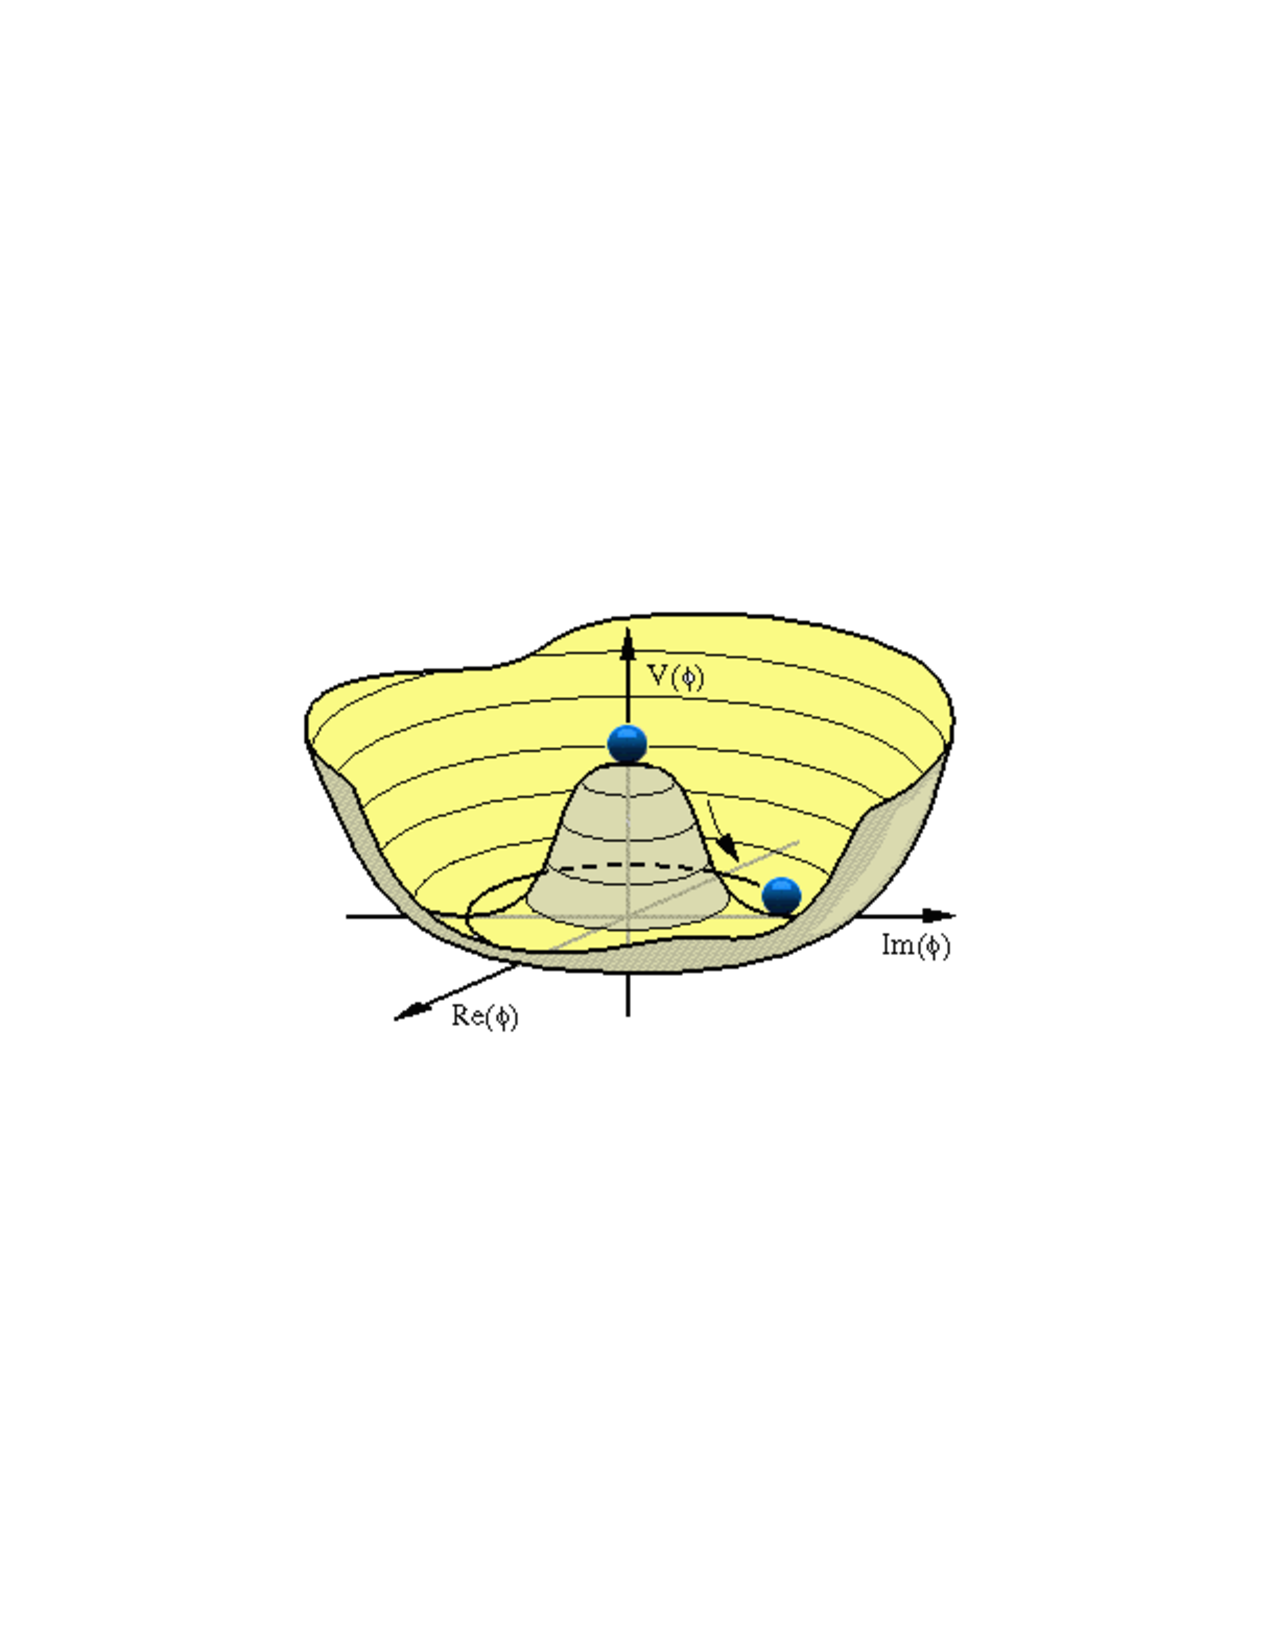
\includegraphics[width=0.5\textwidth]{Figures/Basic_Diagrams/higgs-potential.pdf}
  \caption{A visual representation of the Higgs potential} \label{fig:higgs_potential}
\end{figure}

\noindent if $\mu^{2}>0$ the shape of the potential no longer has a
mimium at $\langle\phi\rangle = 0$.  Figure \ref{fig:higgs_potential}
shows a plot of the potential energy of $\phi$ in terms of each of its
components.  The new minimum potential energy
occurs at:

\begin{equation}\label{eq:abelian_higgs_mechanism_potential_min}
\langle\phi\rangle = \phi_{0} = \left(\frac{\mu^{2}}{\lambda}\right)^{1/2}
\end{equation}

\noindent and while the field has a ground state at the zero potential
point it is in an unstable equilibrium.  Any quantum fluctuation about
this point will take the field into the lower energy configuration
with a ground state about the new minimum.  When the Langrangian is
expanded about~\ref{eq:abelian_higgs_mechanism_potential_min}, the
field, $\phi$ is rewritten as: 

\begin{equation}\label{eq:abelian_higgs_mechanism_expanded_phi}
\phi(x) = \phi_{0} + \frac{1}{\sqrt{2}}(\phi_{1}(x) + i\phi_{2}(x)
\end{equation}

\noindent the potential term, $V(x)$, then becomes:

\begin{equation}\label{eq:abelian_higgs_mechanism_expanded_pot}
V(x) = -\frac{1}{2\lambda}\mu^{4} +
\frac{1}{2}\cdot2\mu^{2}\phi_{1}^{2} + \mathcal{O}(\phi_{i}^{3})
\end{equation}

\noindent where we can notice that $\phi_{1}$ has acquired a mass term
with, $m = \sqrt{2}\mu$, while the scalar field $\phi_{2}$ remains
massless, and is known as the Goldstone boson.  The covariant
derivative is also tranformed as:

\begin{equation}\label{eq:abelian_higgs_mechanism_expanded_covDer}
|D_{\mu}\phi|^{2} = \frac{1}{2}(\partial_{\mu}\phi_{1})^{2} +
\frac{1}{2}(\partial_{\mu}\phi_{2})^{2} +
\sqrt{2}e\phi_{0}\cdot~A_{\mu}\partial^{\mu}\phi_{2} +
e^{2}\phi_{0}^{2}A_{\mu}A^{\mu} + ...
\end{equation}

\noindent where cubic and quartic terms of $A_{\mu}$, $\phi_{1}$,
and $\phi_{2}$ have been dropped.  The important term is the last one,
which can be interpreted as a mass term of the vector field, $A_{\mu}$

\begin{equation}\label{eq:abelian_higgs_mechanism_mass_term_Amu}
\Delta\mathcal{L}_{M} =
  \frac{1}{2}m_{A}A_{\mu}A^{\mu} = e^{2}\phi_{0}^{2}A_{\mu}A^{\mu}
\end{equation}

\noindent where $m_{A} = 2e^{2}\phi_{0}^{2}$, has arisen from
consequences of a non-zero vacuum expectation value of the $\phi$
field.  The remaining, massless Godlstone boson, $\phi_{2}$ is not a
physical particle, but rather a consequence of the choice of guage.
This is illustrated when we can use the $U(1)$ guage symmetry to rotate
the field $\phi(x)$ such that the field disapears.  

\begin{equation}\label{eq:abelian_higgs_mechanism_rotate_phi2}
\begin{aligned}
 \phi \rightarrow \phi' & = e^{i\alpha}(\phi_{1} + \phi_{2}) \\
& = (\cos{\alpha} + i\sin{\alpha})(\phi_{1} + \phi_{2}) \\
& = (\phi_{1}\cos{\alpha} - \phi_{2}\sin{\alpha}) +
i(\phi_{1}\sin{\alpha} + \phi_{2}\cos{\alpha}) \\
& = (\phi_{1} - \phi_{2}\tan{\alpha}) + i(\phi_{1}\tan{\alpha} +
\phi_{2})
\end{aligned}
\end{equation}

\noindent Choosing $\alpha = -\tan{\phi_{2}/\phi_{1}}$ will make $\phi'$
 a real quantity and elminate it's imaginary component, $\phi_{2}'$.
 The lagrangian can then be rewritten in terms of the rotated field
 $\phi'$ and see that massless boson is indeed removed from the
 theory.

\begin{equation}\label{eq:abelian_higgs_mechanism_final_lagrangian}
\begin{aligned}
\mathcal{L} & =
\frac{1}{2}(\partial_{\mu}\phi_{1}')(\partial^{\mu}\phi_{1}') -
\frac{1}{2}\cdot~2\mu^{2}\phi_{1}'\phi_{1}' \\
&  -\frac{1}{4}(F^{\mu\nu}F_{\mu\nu}) +
\frac{1}{2}\cdot~e^{2}\phi_{0}^{2}A_{\mu}A^{\nu} \\
&  + \phi_{0}e^{2}\phi_{1}'A_{\mu}A^{\mu} +
\frac{1}{2}e^2\phi_{1}'^{2}A_{\mu}A^{\mu} + \mathcal{O}(\phi'^{3})...
\end{aligned}
\end{equation}

\par The degree of freedom that $\phi_{2}$ represents, is absorbed as
a longitudanal polarization of the $A_{mu}$ field, a forbidden for
massless guage bosons, but necessary for massive bosons.  

\par For this case of an abelian symmetry $U(1)$, it was shown that if a
complex scalar field, which interacts with itself and another vector
field, can gains a non-zero vacuum expectation value.  The Lagrangian can
be expanded about this new mimimum, generating a mass term for the
vector field.  One of the degrees of freedom of the orginial complex
scalar field is then absorbed as a longitudanal polarization state of
the massive vector field.  

\section{The Higgs Mechanism in a non-Abelian Theory}
\label{non_abelian_higgs_mechanism_overview}

\par Before describing the elctroweak guage theory of
$SU(2)\otimes~U(1)$, it will be helpful to see the effects of the
Higgs mechanism for the non-Abelian group, $SU(2)$ by itself.  Consider an
an example of an $SU(2)$ gauge field coupled to a scalar field that
transforms like a real-valued vector under $SU(2)$
transformations~\cite{Peskin_Schroeder}.  The field $\phi$ will have
the form:

\begin{equation}\label{eq:non_abelian_higgs_mechanism_phi}
\phi = 
  \begin{pmatrix}
    \phi_{1} \\
    \phi_{2} \\
    \phi_{3}
    \end{pmatrix}
\end{equation}

\noindent where the components, $\phi_{i}$ are real-valued fields.
The $SU(2)$ transformation for this scalar field will also look like:

\begin{equation}\label{eq:non_abelian_higgs_mechanism_transformation}
\phi \rightarrow e^{i\alpha^{i}T^{i}}\phi
\end{equation}

\noindent where the matrices, $T^{i}$ are defined as:

\tiny
\begin{equation}\label{eq:non_abelian_higgs_mechanism_generators}
iT^{1} = 
  \begin{pmatrix}
    0  &  0  &  0 \\
    0  &  0  &  1 \\
    0  & -1 &  0 
  \end{pmatrix}
\text{   ,    }
T^{2} = 
  \begin{pmatrix}
    0  &  0  & -1 \\
    0  &  0  &  0 \\
    1  &  0  &  0 \\ 
  \end{pmatrix}
\text{   ,   }
T^{3} = 
  \begin{pmatrix}
    0  &   1  &  0 \\
   -1 &   0  &  0 \\
    0  &   0  &  0
  \end{pmatrix}
\end{equation}
\normalsize

\noindent The Lagrangian for this field will feature a Higgs potential
term along with the previously mentioned $SU(2)$ guage fields, $A_{\mu}^{a}$ coupled
to the scalar field, $phi$, and is given by:

\begin{equation}\label{eq:non_abelian_higgs_mechanism_lagrangian}
\mathcal{L} = -\frac{1}{4}F_{\mu\nu}^{a}F^{a\mu\nu}+ |D_{\mu}\phi|^{2}
+ \mu^{2}\phi^{\ast}\phi - \frac{\lambda}{4}(\phi^{\ast}\phi)^{2}
\end{equation}

\noindent where $F_{\mu}{\nu}^{a}$, the field strength tensor is
defined as:

\begin{equation}\label{eq:non_abelian_higgs_mechanism_field_strength_tensor}
F_{\mu\nu}^{a} = (\partial_{\mu}A_{\nu}^{a}
- \partial_{\nu}A_{\mu}^{a}) + g\epsilon^{abc}A_{\mu}^{b}A_{\nu}^{c}
\end{equation}

\noindent and the covariant derivative is defined as:

\begin{equation}\label{eq:non_abelian_higgs_mechanism_covariant_derivative}
D_{\mu} = (\partial_{\mu} + igA_{\mu}^{a}T^{a})\phi
\end{equation}

\par Similarly to the Abelian case, the Higgs potential will induce a
spontaneous symmetry breaking, and one of the components of the field
$\phi$ will gain a vacuum expectation value.  After this breaking and
expanding around the ground state potential, the
field $\phi$ will have the form:

\begin{equation}\label{eq:non_abelian_higgs_mechanism_phi_broken}
\phi = \frac{1}{\sqrt{2}}
  \begin{pmatrix}
    0 \\
    0 \\
    v + h
    \end{pmatrix}
\end{equation}

\noindent There has been no loss in generality in assuming this form
since, similarly to the abelian case, we can use the gauge symmetry of
$SU(2)$ to rotate the field into this configuration.  Goldstone's
theorem tells us that we should expect two massive gague bosons
corresponding to the $T^{1}$, and $T^{2}$ generators, while the
$T^{3}$ generator will correspond to a massless gauge boson, since
$\phi$ is still invariant under $T^{3}$ transformations. 

\par As in the Abelian case, the mass terms for the gauge bosons are
generated from the covariant derivative term, $|D_{\mu}\phi|^{2}$

\begin{equation}\label{eq:non_abelian_higgs_mechanism_covariant_derivative_on_phi}
\begin{aligned}
D_{\mu}\phi & = \frac{1}{\sqrt{2}}\left(~\partial_{\mu} + gA_{\mu}^{1}
  \begin{pmatrix}
    0  &  0  &  0 \\
    0  &  0  &  1 \\
    0  & -1 &  0 
  \end{pmatrix}
  + gA_{\mu}^{2}
  \begin{pmatrix}
    0  &  0  & -1 \\
    0  &  0  &  0 \\
    1  &  0  &  0 \\ 
  \end{pmatrix}
+ gA_{\mu}^{3}
  \begin{pmatrix}
    0  &   1  &  0 \\
   -1 &   0  &  0 \\
    0  &   0  &  0
  \end{pmatrix}
\right)
  \begin{pmatrix}
    0 \\
    0 \\
    v + h
  \end{pmatrix} \\
 & = \frac{1}{\sqrt{2}}
  \begin{pmatrix}
    0 \\
    0 \\
    \partial_{\mu}
  \end{pmatrix}
  + \frac{gA_{\mu}^{1}}{\sqrt{2}}
  \begin{pmatrix}
    0 \\
    v+h \\
    0
  \end{pmatrix}
  - \frac{gA_{\mu}^{2}}{\sqrt{2}}
  \begin{pmatrix}
    v+h \\
    0 \\
    0
    \end{pmatrix} \\
 & = \frac{1}{\sqrt{2}}
  \begin{pmatrix}
    g(v+h)A_{\mu}^{1} \\
    g(v+h)A_{\mu}^{2} \\
    \partial_{\mu}h
  \end{pmatrix}
\end{aligned}
\end{equation}

\noindent Therefore

\begin{equation}\label{eq:non_abelian_higgs_mechanism_covariant_derivative_sq}
|D_{\mu}\phi|^{2} = \frac{1}{2}\partial_{\mu}h\partial^{\mu}h +
\frac{g^{2}v^{2}}{2}\left( (A_{\mu}^{1})^{2} + (A_{\mu}^{2})^{2} \right) +
\frac{g^{2}}{2}(h^{2}+2hv)\left( (A_{\mu}^{1})^{2} + (A_{\mu}^{2})^{2} \right)
\end{equation}

\par This theory produces two massive bosons, $A_{\mu}^{1}$ and
$A_{\mu}^{2}$, both with mass, $m_{A} = gv$.  These fields have $h$,
and $h^2$ couplings to the Higgs boson.  The third guage field,
$A_{\mu}^{3}$, remains massles and is not coupled to the Higgs field.
This model is beginning to resemble a description of electroweak
physics, however, a third massive boson is necessary, as is a new
gague symmetry in order to generate it.  That is the subject of the
next section.  

\section{Glashow Weinberg Salam Theory}
\label{ewk_overview}

\par Glashow, Weinberg, and Salam published their theory unifying
elctromagnetic and weak forces in the
1960s~\cite{th:Weinberg_ModelOfLeptons}~\cite{th:Glashow_PartialSymmetries}~\cite{th:Salam_EWKInteractions}.
It begins with the requirement of a $SU(2)_{L}\otimes~U(1)$
symmetry and incorporates the Higgs mechanism to give mass to the guage bosons
of the weak force.  As described earlier, the $U(1)$ symmetry requires
introducing a vector field, which will be labeled $B_{\mu}$, and an interaction term, which
is absorbed into the covariant derivative, $D_{\mu}$.  The
transformation will also be paramaterized with a with a quantum
number, $Y$, known as hypercharge.  The $SU(2)$
symmetry requires the introduction of three new 
vector fields, which will be labeled $W_{\mu}^{i}, i = 1, 2, 3$.  The
quantum number associated with this gauge group is known as isospin,
and is determined by the $T^{3}$ operator, acting on an $SU(2)$
doublet on the third generator of the group. The $SU(2)\otimes~U(1)$
transformation, $U(x)$, will then be give by:   

\begin{equation}\label{eq:ewk_su2_su1_transformation}
U(x) = e^{i\alpha^{a}(x)\tau^{a}}e^{iY\alpha(x)/}
\end{equation}

\noindent where $\tau^{a} = \sigma^{a}/2$, the Pauli matrices,
\ref{eq:pauli_matrices}.  These gauge fields will be coupled, via the
covariant derivative, to a doublet of complex scalar fields $\phi$,
with hypercharge $Y=+1/2$.  A Higgs potential will be added to 
generate the spontaneous symmetry breaking that will give mass to
three of the guage fields, and leave one massless.  In order to
preserve the $SU(2)_{L}\otimes~U(1)$ symmetry, the new covariant 
derivative will take the form:

\begin{equation}\label{eq:ewk_covariant_derivative}
D_{\mu} = (\partial_{\mu} - igW_{\mu}^{a}\tau^{a} -
\frac{i}{2}g'B_{\mu})
\end{equation}

\par The subscript L on $SU(2)_{L}$ refers to the experimental
results that the weak force violates parity maximally, by only
interacting with the left-handed chiral component of a field.  Right
versus left chiralty is determined by whether the spin of a particle
is aligned or anti-aligned with its direction of motion, and in
general a particle is represented by a linear combination of its right and
left handed components.  This idea was first proposed by Chen Ning
Yang and Tsung-Dao Lee, in the 1950s.  Their ideas were validated by
the experimental discovery of partiy violation in 1957, through the beta decays of Cobalt
60 atoms by C.S Wu.  That same year, Yang and Lee were awrded the
nobel prize for their insight~\cite{th:YangLee_NobelPrize}.  In this
model, then, the left-handed components of the particles participate
in the weak interaction and are formed into doublets, while the right handed
components are singlets, and will only interact with the
electromagnetic field, $B_{\mu}$.  The quantum numbers of the doublet
will be given by +1/2 for the upper component of the $SU(2)$ doublet,
and -1/2 for the lower component.  The fermion content of this theory
is then given by:

\begin{equation}\label{eq:ewk_fermion_doublets}
\begin{aligned}
&\binom{\nu_{L}}{e_{L}}, e_{R} \\
&\binom{u_{L}}{d_{L}}, u_{R}, d_{R} 
\end{aligned}
\end{equation}

\noindent where the right handed neutrino, $\nu_{R}$ has been ommited,
since it has zero charge, and isospin, and therefore does not
participate in any of the interactions of this theory.  The complete
Lagrangian is given by a sum of free particle terms for  massless bosons,
fermions, and Higgs scalar fields; the Higgs potential; and a Yukawa
coupling term between the fermions and the Higgs, which generates
their masses. 

\begin{equation}\label{eq:ewk_lagrangian_simple}
\mathcal{L}_{GWS} = \mathcal{L}_{Boson KE} + \mathcal{L}_{Higgs} +
\mathcal{L}_{Fermion KE} + \mathcal{L}_{Yukawa} 
\end{equation}

\noindent The Higgs potential will have the form:
\begin{equation}\label{eq:ewk_higgs_lagrangian_term}
\mathcal{L}_{Higgs} = (D_{\mu}\phi)^{\dagger}(D^{\mu}\phi)
+\mu^{2}\phi^{\dagger}\phi - \lambda(\phi^{\dagger}\phi)^{2}
\end{equation}

\noindent The Higgs potential will break the symmetry of
the Lagrangian when one of the four degrees of freedom in the
complex scalar doublet, $\phi$, spontaneously acquires a
vacuum expectation value.  In this case, it will generate
three massive gauge bosons, one massless gauge boson, and a massive
scalar field.  After gaining a vacuum expectation value, and expanding
about this value, the scalar fields will have the form:

\begin{equation}\label{eq:ewk_phi_vev}
\langle\phi\rangle = \frac{1}{\sqrt{2}}\binom{0}{v+h}
\end{equation}

\noindent where no loss of generality has occured since we are always
able to rotate into this form through the appropriate gauge
transformations, similar to what was descibed in the Abelian case.  It
should also be noted that this form is not invariant to any of the
individual generators $t^{a}$, however $\phi$ will be invariant to a
combination of $T^{3}+Y$ generators.  Per Goldstone's thereom, we
should expect this linear combination of fields to be the massless
vector boson after symemtry breaking.  The massless eigenstate will be
the electromagnetic field, $A_{\mu} \sim~A_{\mu}^{3} + B_{\mu}$.  The
electric charge quantum number, $Q$, is then defined as 
\begin{equation}\label{ewk_Q_quantum_number}
Q = T^{3}+Y
\end{equation}

\par As before, the generation of the masses for the guage bosons are
generated by the interaction of their fields with the Higgs field via
the covariant derivative.  

\begin{equation}\label{eq:ewk_covariant_derivative_acting_on_phi}
\begin{aligned}
D_{\mu}\phi & = \frac{1}{\sqrt{2}}\left( \partial_{\mu}
  - \frac{ig}{2}A_{\mu}^{1} 
  \begin{pmatrix}
    0  &  1 \\
    1  &  0
  \end{pmatrix}
  - \frac{ig}{2}A_{\mu}^{2} 
  \begin{pmatrix}
    0  & -i \\
    i  &  0
  \end{pmatrix}
  - \frac{ig}{2}A_{\mu}^{3} 
  \begin{pmatrix}
    1  &   0 \\
    0  & -1
  \end{pmatrix}
\right)\binom{0}{v+h} \\ \\
& = \frac{1}{\sqrt{2}}\binom{(\frac{g}{2}(v+h)A_{\mu}^{2}) +
  i(\frac{g}{2}(v+h)A_{\mu}^{1})}{\partial_{\mu} +
  i(\frac{1}{2}(v+h)(gA_{\mu}^{3}-g'B_{\mu}))}
\end{aligned}
\end{equation}

\noindent Taking the dot product of this with its hermitian conjugate
gives the $|D_{\mu}\phi|^{2}$ term:

\begin{equation}\label{eq:ewk_partial_phi_squared}
\begin{aligned}
|D_{\mu}\phi|^{2} = & \frac{1}{2}\partial_{\mu}h\partial^{\mu}h +
\frac{1}{2}\frac{g^{2}v^{2}}{4}( (A_{\mu}^{1})^{2} + (A_{\mu}^{2})^{2}
) +\frac{v^{2}}{4}(gA_{\mu}^{3}-g'B_{\mu})^{2}  \\
 & + \frac{1}{2}{g^{2}}{4}(h^{2}+2vh)( (A_{\mu}^{1})^{2} +
 (A_{\mu}^{2})^{2} ) +
 \frac{1}{2}\frac{1}{4}(h^{2}+2vh)(gA_{\mu}^{3}-g'B_{\mu}) 
\end{aligned}
\end{equation}

\noindent From equation~\ref{eq:ewk_partial_phi_squared} we
can identify three massive and one massless guage bosons,
corresponding the the charged and nuetral weak currents, and the
elctromagnetic current.  

\begin{equation}\label{eq:ewk_boson_masses}
\begin{aligned}
W_{\mu}^{\pm} & = \frac{1}{\sqrt{2}}(A_{\mu}^{1} \mp iA_{\mu}^{2}) 
&\text{  with mass  }  m_{W} &= g\frac{v}{2}\text{;} \\
Z_{\mu}^{0} & = \frac{1}{\sqrt{g^{2}+g'^{2}}}(gW_{\mu}^{3}-g'B_{\mu})  
&\text{  with mass  }  m_{Z} &= \frac{v}{2}\sqrt{g^{2}+g'^{2}}\text{;}  \\
A_{\mu} & = \frac{1}{\sqrt{g^{2}+g'^{2}}}(gW_{\mu}^{3}+g'B_{\mu}) 
&\text{  with mass  }  m_{A} &= 0 \text{;} 
\end{aligned}
\end{equation}

\noindent where the last field, $A_{\mu}$ is absent from the covariant
derivative term, but already identified as the massless gauge boson of
the theory due to it's gauge invariance under a $T^{3}+Y$ rotation.
Using these definitions the covariant derivative has the following
form:

\begin{equation}\label{eq:ewk_covariant_derivative_mass_eigenstates}
\begin{aligned}
D_{\mu} & = \partial_{\mu} - \frac{ig}{\sqrt{2}}(W^{+}T^{+} + W^{-}T^{-}) \\
  &  - \frac{i}{\sqrt{g^{2}+g'^{2}}}Z_{\mu}^{0}(gT^{3} - g'Y) -
    \frac{gg'}{\sqrt{g^{2}+g'^{2}}}A_{\mu}(T^{3}+Y) 
\end{aligned}
\end{equation} 

\noindent where $T^{\pm} = \frac{1}{2}(\sigma^{1}\pm\sigma^{2})$.  From
this form, we can identiy the fundamental electric charge, $e$, as

\begin{equation}\label{eq:ewk_electric_charge}
e = \frac{gg'}{\sqrt{g^{2}+g'^{2}}}
\end{equation}

The similarity in the forms between $Z_{\mu}^{0}$ and $A_{\mu}$
suggest that their relationship can be expressed in a simpler form, as
the rotation of underlying guage fields $A_{\mu}^{3}$ and $B_{\mu}$
through the weak mixing angle, $\theta_{W}$

\begin{equation}\label{eq:weak_mixing_matrix}
\binom{Z_{\mu}^{0}}{A_{\mu}} = 
\begin{pmatrix}
    \cos{\theta_{W}} & -\sin{\theta_{W}} \\
    \sin{\theta_{W}}  &  \cos{\theta_{W}}
  \end{pmatrix}
\binom{A_{\mu}^{3}}{B_{\mu}}
\end{equation}

\noindent where $\tan{\theta_{W}} = \frac{g'}{g}$.  Expanding
\ref{eq:weak_mixing_matrix}, we have the definitions of the
$Z_{\mu}^{0}$ and $A_{\mu}$ fields in terms of $\theta_{W}$

\begin{equation}\label{eq:ewk_Z_A_defined_with_thetaW}
\begin{aligned}
Z_{\mu}^{0} &= A_{\mu}^{3}\cos{\theta_{W}} - B_{\mu}\sin{\theta_{W}}
\\
A_{\mu} & = A_{\mu}^{3}\sin{\theta_{W}} + B_{\mu}\cos{\theta_{W}}
\end{aligned}
\end{equation}

\noindent The weak mixing angle, $\theta_{W}$, also provides a
simple relationship between the $W_{\mu}^{\pm}$ and $Z_{\mu}^{0}$
fields:

\begin{equation}\label{eq:ewk_mz_is_mwcosthetaW}
m_{W} = m_{Z}\cos{\theta_{W}}
\end{equation}

\noindent The covariant derivative, $D_{\mu}$ is also rewritten in
terms of the mass eignenstates of the gauge fields

\begin{equation}\label{eq:ewk_covariant_derivative_mass_eigenstates}
D_{\mu} = (\partial_{\mu} - \frac{ig}{\sqrt{2}}(W_{\mu}^{+} +
W_{\mu}^{-}T^{-}) -
\frac{ig}{\cos{\theta_{W}}}Z_{\mu}^{0}(T_{3}-sin^{2}{\theta_{W}}Q) -
ieA_{\mu}Q)
\end{equation}

\noindent where $g = e/\cos{\theta_{W}}$.  The square of the covariant
derivative is then written as

\begin{equation}\label{eq:ewk_covariant_derivative_squared_mass_eigenstates}
\begin{aligned}
|D_{\mu}|^{2} &= \frac{1}{2}\partial_{\mu}h\partial^{\mu}h +
\frac{1}{2}m_{W}^{2}W_{\mu}^{+}W^{\mu+} +
\frac{1}{2}m_{W}^{2}W_{\mu}^{-}W^{\mu-} +
\frac{1}{2}m_{Z}^{2}Z_{\mu}^{0}Z^{\mu0} \\
& + (\frac{h^{2}}{v^{2}} + \frac{h}{v})[
    \frac{1}{2}m_{W}^{2}(W_{\mu}^{+}W^{\mu+}+W_{\mu}^{-}W^{\mu-}) +
    \frac{1}{2}m_{Z}^{2}Z_{\mu}^{0}Z^{\mu0}]
\end{aligned}
\end{equation} 
\\
\par With the form of the covariant derivative in place, the
fermionic kinematic term of the Lagrangian can be described.  As
mentioned earlier, the masses of the fermions in the model will be
generated by the Yukawa interaction term with the Higgs, so this
term only involves the covariant derivatives acting on the left-handed
doublet and right-handed singlet states of this model.  

\begin{table}[h]
  \begin{center}
%                              vl  el  er  ul  dl  ur  dr
  \begin{tabular}{ | l | c | c | c | c | c | c | c | } \hline
    & $\nu_{L}$ & $e_{L}$ & $e_{R}$ & $u_{L}$ & $d_{L}$ & $u_{R}$ &
    $d_{R}$ \\ \hline
    Isospin & +1/2 & -1/2 & 0 & +1/2 & -1/2 & 0 & 0 \\ \hline
    Hypercharge & -1/2 & -1/2 & -1 & +1/6 & 1/3 & 2/3 & -1/3 \\ \hline
    Electric Charge & 0 & -1 & -1 & 2/3 & -1/3 & 2/3 & -1/3 \\ \hline
  \end{tabular}
  \caption{ The quantum numbers Isospin and Hypercharge are assigned for each of the $SU(2)$ and
      $U(1)$ symmetries respectively}
    \label{tab:ewk_fermion_quantum_numbers}
  \end{center}
\end{table} 

\noindent The quantum number assignments for the leptons, which are
chosen in order to reproduce the known values of their electric
charges, are shown in table~\ref{tab:ewk_fermion_quantum_numbers}.
The values  of these quantum numbers enter into the covariant
derivative via the  $Z_{\mu}^{0}$ term of equation
\ref{eq:ewk_covariant_derivative_mass_eigenstates}.  The fermionic
kinetic energy term of the Lagrangian is given by:

\begin{equation}\label{eq:ewk_fermionic_lagrangian_term}
\begin{aligned}
\mathcal{L}_{Fermion} =&~ \bar{E}_{L}(i\gamma^{u}D_{\mu})E_{L} +
\bar{e}_{R}(i\gamma^{u}D_{\mu})e_{R} \\
&~ \bar{Q}_{L}(i\gamma^{u}D_{\mu})Q_{L} +
\bar{u}_{R}(i\gamma^{u}D_{\mu})u_{R} +
\bar{d}_{R}(i\gamma^{u}D_{\mu})d_{R}
\end{aligned}
\end{equation} 

\noindent Expanding the covariant term for the left-handed electron
shows its explicit coupling to the guage boson fields. 

\begin{equation}\label{eq:ewk_eLeft_lagrangian_term}
\begin{aligned}
\mathcal{L}_{E_{L}} =&~ 
\begin{pmatrix}
  \bar{\nu_{L}} & \bar{e_{L}} 
\end{pmatrix}
\left( (i\gamma^{\mu}(\partial_{\mu} -
  \frac{ig}{\sqrt{2}}(W_{\mu}^{+}T^{+} + W_{\mu}^{-}T^{-}) -
  \frac{ig}{\cos{\theta_{W}}}Z_{\mu}^{0}(T^{3}-\sin^{2}{\theta_{W}}Q)
  - ieA_{\mu}Q)~)~\right)\binom{\nu_{L}}{e_{L}} \\
=&~\bar{\nu_{L}}i\gamma^{\mu}\partial_{\mu}\nu_{L} +
\bar{e_{L}}i\gamma^{\mu}\partial_{\mu}e_{L}
+\frac{ig}{\sqrt{2}}W_{\mu}^{+}\bar{\nu_{L}}\gamma^{\mu}e +
\frac{ig}{\sqrt{2}}W_{\mu}^{-}\bar{e_{L}}\gamma^{\mu}\nu_{L} \\
&~+\frac{ig}{\cos{\theta_{W}}}\bar{\nu_{L}}(1/2)\gamma^{\mu}\nu_{L} +
\frac{ig}{\cos{\theta_{W}}}\bar{e_{L}}\gamma^{\mu}(-1/2 +
\sin^{2}{\theta_{W}}(+1))e_{L} + (ie)\bar{e_{L}}\gamma^{\mu}A_{\mu}(-1)
\end{aligned}
\end{equation}

\noindent All of the terms will be combined with the final,
spontaneously broken GWS Lagranian at the end of this section.  

\par The final term to discuss in the theory, before combing all of
the results, is the Yukawa interaction term between the fermion fields
and the Higgs.  For the electron, this term takes the form:

\begin{equation}\label{eq:ewk_yukawa}
\begin{aligned}
\mathcal{L}_{Yukawa} =&~ -\lambda_{e}\bar{E_{L}}\cdot\phi~e_{R} -
\lambda_{e}E_{L}\cdot\phi~\bar{e_{R}} \\
=&~ -\frac{\lambda_{e}}{\sqrt{2}}(v+h)(\bar{e_{L}}e_{R} +
  e_{L}\bar{e_{R}}) \\
=&~ --\frac{\lambda_{e}v}{\sqrt{2}}(\bar{e_{L}}e_{R} +
  e_{L}\bar{e_{R}}) + -\frac{\lambda_{e}}{\sqrt{2}}(\bar{e_{L}}e_{R} +
  e_{L}\bar{e_{R}})h
\end{aligned}
\end{equation}

\noindent where the mass of the electron is identified as $m_{e} =
\frac{\lambda_{e}v}{\sqrt{2}}$.  In order to generate the masses of
the particles, each fermion has its own unique $\lambda$ value.  So
while the Higgs mechanism is able to generate the masses in a way that
preserves the underlying $SU(2)\otimes~U(1)$ symmetry, it does not
explain the heirarchy of masses since each $\lambda$ value is unique
to each lepton.  The second term in last equation of
~\ref{eq:ewk_yukawa} is the coupling of the Higgs particle, $h$, to
the fermions.  The coupling is proportional to the mass of the
particle.  The largest of these is to the top quark, with $m_{t} =
73.21 \pm 0.51 \pm 0.71 GeV$.

\par The Yuakawa coupling for the quarks is necessarily modified when
additional quarks besides the $u$ and $d$ are added to the theory.
This is because there can be additional coupling terms that mix
generations.  This occurs when the mass eigenstate of the quarks is
not the same as the interaction eigenstate.  The modification requires
the expansion of the $u_{L}$ and $d_{L}$ components into a vector of
left handed quarks.  If we let

\begin{equation}\label{eq:ewk_quark_vector}
\begin{aligned}
u_{L}^{i} = (u_{L}, c_{L}, t_{L}) &,                 & d_{L}^{i} = (d_{L}, s_{L}, b_{L})
\end{aligned}
\end{equation}

\noindent represent the up and down-type quarks in the orginal weak
interaction basis, then the vectors, $u_{L}^{i}$' and $d_{L}^{i}$',
can be defined as the diagonlized basis for the Higgs coupling.  They
are related through a unitary transformation.  

\begin{equation}\label{eq:ewk_quark_transformaitons}
\begin{aligned}
u_{L}^{i} = U_{u}^{ij}u_{L}^{j\prime} &,                 & d_{L}^{i} = U_{d}^{ij}d_{L}^{j\prime}
\end{aligned}
\end{equation}

\noindent The interaction terms with the charged gauge boson currents
must then be rewritten as

\begin{equation}\label{eq:ewk_ckm_intro}
J_{W}^{\mu+} = \frac{1}{\sqrt{2}}\bar{u_{L}^{i}}\gamma^{\mu}d_{L}^{i}
=
\frac{1}{\sqrt{2}}\bar{u_{L}^{i\prime}}\gamma^{\mu}(U_{u}^{\dagger}U_{d})d_{L}^{j\prime}
= \frac{1}{\sqrt{2}}\bar{u_{L}^{i\prime}}\gamma^{\mu}V_{ij}d_{L}^{j\prime}
\end{equation}

\noindent where $V_{ij}$ is the 3x3 Cobibbo-Kobayashi-Maskawa (CKM) matrix
describing the mixing among six
quarks~\cite{th:CKM_matrix_C}~\cite{th:CKM_matrix_KM}.  It is an
extension of the Glashow-Iliopoulos-Maiaini mechanism, which was a 2x2
matrix that predicted the existence of a fourth quark, the charm quark.  The GIM
mechanism was an attempt to suppress flavor-changing-neutral currents,
which occur at LO in a three-quark model, but not in a four-quark
model.  The CKM matrix, however, was motivated by an attempt to
explain $CP$ violation in the weak interaction.  At the time of its
publication, the bottom and top quarks were not predicted.  After
these were discovered, they were awarded the nobel prize in physics in
2008.  

\par At this point, all the of the pieces are ready to write down the
GWS Lagrangian, after the Higgs mechanism has spontaneously broken the
$SU(2)\otimes~U(1)$ symmetry.

\begin{equation}\label{eq:ewk_lagrangian_unbroken}
\begin{aligned}
\mathcal{L}_{Unbroken} = &~ -\frac{1}{4}A_{\mu\nu}^{a}A^{\mu\nu~a} -
\frac{1}{4}F_{\mu\nu}F^{\mu\nu} \\
&~ + |D_{\mu}\phi|^{2} + \mu^{2}(\phi^{\dagger}\phi) - \lambda(\phi^{\dagger}\phi)^{2} \\
&~ + \bar{E_{L}}(i\gamma^{\mu}D_{\mu})E_{L} + \text{ similar terms for }
    e_{R}, U_{L}, u_{R}, d_{R} \\
&~ -\lambda_{e}\bar{E_{L}}\cdot\phi~e_{R} + h.c. + \text{ similar
  terms for } e_{R}, U_{L}, u_{R}, d_{R}
\end{aligned}
\end{equation}

\begin{equation}\label{eq:ewk_lagrangian_broken}
\begin{aligned}
\mathcal{L}_{GWS} = &~ -\frac{1}{4}(Z_{\mu\nu}^{0})^{2} -
\frac{1}{2}(W_{\mu\nu}^{+}W_{\mu\nu}^{-}) -
\frac{1}{4}(F_{\mu\nu})^{2}  \\
&~ + ig\cos{\theta_{W}}\left( (W_{\mu}^{-}W_{\nu}^{+} -
  W_{\nu}^{-}W_{\mu})\partial^{\mu}Z^{0\nu} +
  W_{\mu\nu}^{+}W^{-\mu}Z^{0\nu} + W_{\mu\nu}^{-}W^{+\mu}Z^{0\nu}
\right) \\ 
&~ + ie\left(
  (W_{\mu}^{-}W_{\nu}^{+}-W_{\nu}^{-}W_{\mu}^{+})\partial^{\mu}A^{\nu}
  + W_{\mu\nu}^{+}W^{-\mu}A^{\nu} - W_{\mu\nu}^{-}W^{+\mu}A^{\nu}
\right)\\
&~ + g^{2}\cos^{2}{\theta_{W}}\left(
  W_{\mu}^{+}W_{\nu}^{-}Z^{0\mu}Z^{0\nu} -
  W_{\mu}^{+}W^{-\mu}Z_{\nu}^{0}Z^{0\nu} \right) \\
&~ + g^{2}\left( W_{\mu}^{+}W_{\mu}^{-}A^{\mu}A^{\nu} -
  W_{\mu}^{+}W^{-\mu}A_{\nu}A^{\nu} \right) \\
&~ + ge\cos{\theta_{W}}\left( W_{\mu}^{+}W_{\nu}^{-}(Z^{0\mu}A_{\nu} +
  Z^{0\nu}A^{\mu}) - 2W_{\mu}^{+}W^{-\mu}A^{\nu} \right) \\
&~ + \frac{1}{2}g^{2}(W_{\mu}^{+}W_{\nu}^{-})(W^{+\mu}W^{-\nu} -
W^{+\nu}W^{-\mu}) \\
&~ + \frac{1}{2}\partial_{\mu}h\partial^{\nu}h - v^{2}{\lambda}h^{2} +
\frac{1}{2}m_{W}^{2}W_{\mu}^{+}W^{+\mu} +
\frac{1}{2}m_{W}^{2}W_{\mu}^{-}W^{-\mu} +
\frac{1}{2}m_{Z}^{2}Z_{\mu}^{0}Z^{0\mu} \\
&~ + (\frac{h^{2}}{v^{2}} + \frac{h}{v})\left(
  \frac{1}{2}m_{W}^{2}(W_{\mu}^{+}W^{+\mu} + W_{\mu}^{-}W^{-\mu}) +
  \frac{1}{2}m_{Z}^{2}Z_{\mu}^{0}Z^{0\mu} \right) - {\lambda}vh^{3} - \frac{1}{4}{\lambda}h^{4} \\
&~ + \bar{E_{L}}(i\gamma^{\mu}\partial_{\mu})E_{L} +
\bar{e_{R}}(i\gamma^{\mu}\partial_{\mu})e_{R} +
\bar{Q_{L}}(i\gamma^{\mu}\partial_{\mu})Q_{L} +
\bar{u_{R}}(i\gamma^{\mu}\partial_{\mu})u_{R}  +
\bar{d_{R}}(i\gamma^{\mu}\partial_{\mu})d_{R} \\ 
&~ + g(W_{\mu}^{+}J_{W}^{\mu+} + W_{\mu}^{-}J_{W}^{\mu-} +
Z_{\mu}^{0}J_{Z}^{\mu}) + eA_{\mu}J_{EM}^{\mu} \\
&~ -\frac{\lambda_{e}v}{\sqrt{2}}(\bar{e_{L}}e_{R}+\bar{e_{R}}e_{L}) +
-\frac{\lambda_{e}h}{\sqrt{2}}(\bar{e_{L}}e_{R}+\bar{e_{R}}e_{L}) \\
&~ -\frac{\lambda_{u}v}{\sqrt{2}}(\bar{u_{L}}u_{R}+\bar{u_{R}}u_{L}) +
-\frac{\lambda_{u}h}{\sqrt{2}}(\bar{u_{L}}u_{R}+\bar{u_{R}}u_{L})  \\
&~ -\frac{\lambda_{d}v}{\sqrt{2}}(\bar{d_{L}}d_{R}+\bar{d_{R}}d_{L}) +
-\frac{\lambda_{d}h}{\sqrt{2}}(\bar{d_{L}}d_{R}+\bar{d_{R}}d_{L})  \\
\end{aligned}
\end{equation}

\noindent where the currents of the electroweak interaction,
$J_{W}^{\mu+}$, $J_{W}^{\mu-}$, $J_{Z}^{\mu}$, $J_{A}^{\mu}$ are
defined as:
\begin{equation}\label{eq:ewk_currents}
\begin{aligned}
J_{W}^{\mu+} =&~ \frac{1}{\sqrt{2}}\left(
  \bar{\nu_{L}}\gamma^{\mu}e_{L} + \bar{u_{L}^{i\prime}}\gamma^{\mu}V_{ij}d_{L}^{j\prime}
\right) \\ 
J_{W}^{\mu-} =&~ \frac{1}{\sqrt{2}}\left(
  \bar{e_{L}}\gamma^{\mu}\nu_{L} +
    \bar{d_{L}^{i\prime}}\gamma^{\mu}V_{ij}u_{L}^{j\prime} \right) \\
J_{Z}^{\mu} =&~ \frac{1}{\cos{\theta_{W}}}(
  \bar{\nu_{L}}\gamma^{\mu}(+1/2)\nu_{L} +
  \bar{e_{L}}\gamma^{\mu}(-1/2+\sin^{2}{\theta_{W}})e_{L} +
  \bar{e_{R}}\gamma^{\mu}\sin^{2}{\theta_{W}}e_{R} \\
&~ + \bar{u_{L}}\gamma^{\mu}(1/2-2/3sin^{2}{\theta_{W}})u_{L} +
\bar{u_{R}}\gamma^{\mu}(-2/3sin^{2}{\theta_{W}})u_{R} \\
&~ + \bar{d_{L}}\gamma^{mu}(-1/2+1/3sin^{2}{\theta_{W}})d_{L} +
\bar{d_{R}}\gamma^{\mu}(1/3sin^{2}{\theta_{W}})d_{R} ) \\
J_{EM}^{\mu} =&~ \bar{e_{L,R}}\gamma^{\mu}(-1)e_{L,R} +
\bar{u_{L,R}}\gamma^{\mu}(2/3)u_{L,R} + \bar{d_{L,R}}\gamma^{\mu}(-2/3)d_{L,R}
\end{aligned}
\end{equation}



\section{The Standard Model of Particle Physics}
\label{standard_model_overview}

\par The Standard Model of particle physics, extends the GWS model by
incorporating the QCD interaction between the quarks and gluons.  The
symmetry of this theory is that of:
\begin{equation}\label{eq:sm_symmetry}
SU(3)_{C}\otimes~SU(2)_{L}\otimes~U(1)_{\gamma}
\end{equation}

\noindent The Lagrangian of the model is given by 

\begin{equation}\label{eq:sm_lagrangian}
\mathcal{L}_{SM} = \mathcal{L}_{GWS} -
\frac{1}{4}G_{\mu\nu}^{a}G^{a\mu\nu} + g_{S}C_{\mu}^{a}J_{QCD}^{a\mu}
\end{equation}

\noindent where the current for the QCD interaction, $J_{QCD}^{a\mu}$
is defined as:

\begin{equation}\label{eq:sm_qcd_current}
J_{QCD}^{a} = \bar{u^{i}}\gamma^{\mu}t^{a}u^{i} + \bar{d^{i}}\gamma^{\mu}t^{a}d^{i}
\end{equation}

\noindent where $t^{a}$ are the Gell-Mann matrices defined in equation
\ref{eq:gell_man_matrices}.  The field strength tensor for the eight gluon fields,
$G_{\mu\nu}^{a}$, is defined as

\begin{equation}\label{eq:sm_gluon_field_strength_tensor}
G_{\mu\nu}^{a} = (\partial_{\mu}C_{\nu}^{a}
- \partial_{\nu}C_{\mu}^{a}) - g_{S}f^{abc}C_{\mu}^{b}C_{\mu}^{c}  
\end{equation} 

\par The experimental evidence in favor of the SM is compelling.
It has not only been able to describe existing phenomenon to great
precision, but has also predicted the existence of new forms of matter
and interactions among fundamental particles.  The
UA1~\cite{ex:UA1_W}~\cite{ex:UA1_Z} and UA2~\cite{ex:UA2_W}~\cite{ex:UA2_Z}
experiments at CERN, under the leadership of Carlo Rubbia, discovered
the $W$ and $Z$ bosons in 1983.  The experiments observed a handful of
events, in $p\bar{b}$ collisions, at $\sqrt{s}=540\GeV$, and were able
to measure the masses to be $M_{W}\sim~80\GeV$ and
$M_{Z}\sim~95\GeV$.  

\par In the following years, from 1989-2000, the Large
electron-positron (LEP) collider at CERN conducted precision measurments of
the Standard Model~\cite{ex:LEP_Z-Pole}~\cite{ex:LEP-2_W}.  Along with
high-precision measurements on on the $W,Z$ masses:

\begin{equation}\label{eq:lep_WZ_masses}
\begin{aligned}
m_{Z} =&~ 91.1875 \pm 0.0021\GeV \\
m_{W} =&~ 80.376 \pm 0.0033\GeV 
\end{aligned}
\end{equation}  

\begin{figure}
   \centering
   \begin{subfigure}[h]{0.3\textwidth}
     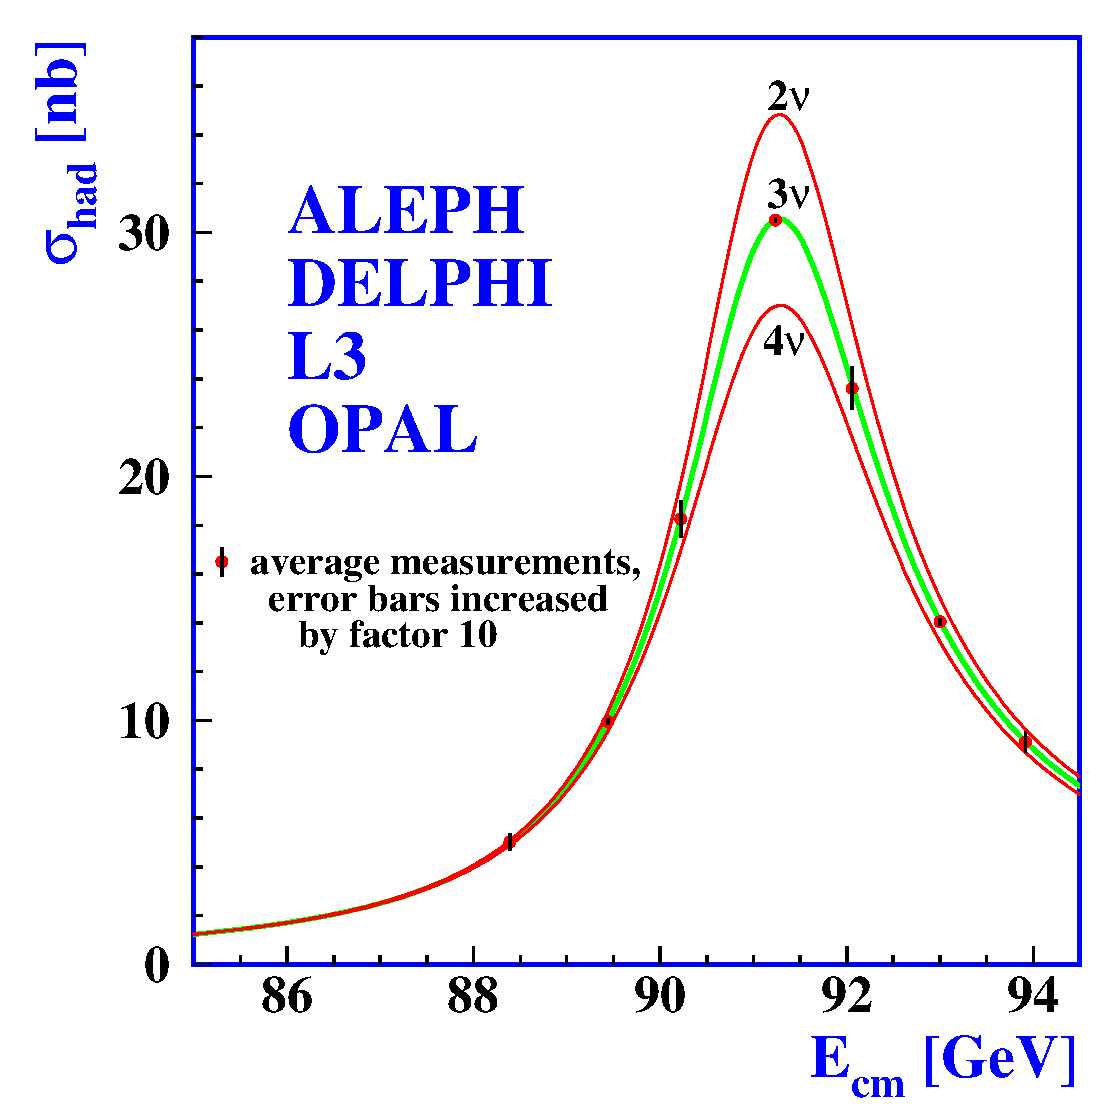
\includegraphics[width=\textwidth]{Figures/Experimental_Results/Nnu.eps}
     \caption{Measurement of the width of $Z$ boson from LEP, comparing the hypotheses of
    2, 3, or 4 neutrino generations} \label{fig:lep_Z_3_families}
   \end{subfigure}
   ~ %add desired spacing between images, e. g. ~, \quad, \qquad, \hfill etc.
      % (or a blank line to force the subfigure onto a new line)
   \begin{subfigure}[h]{0.3\textwidth}
     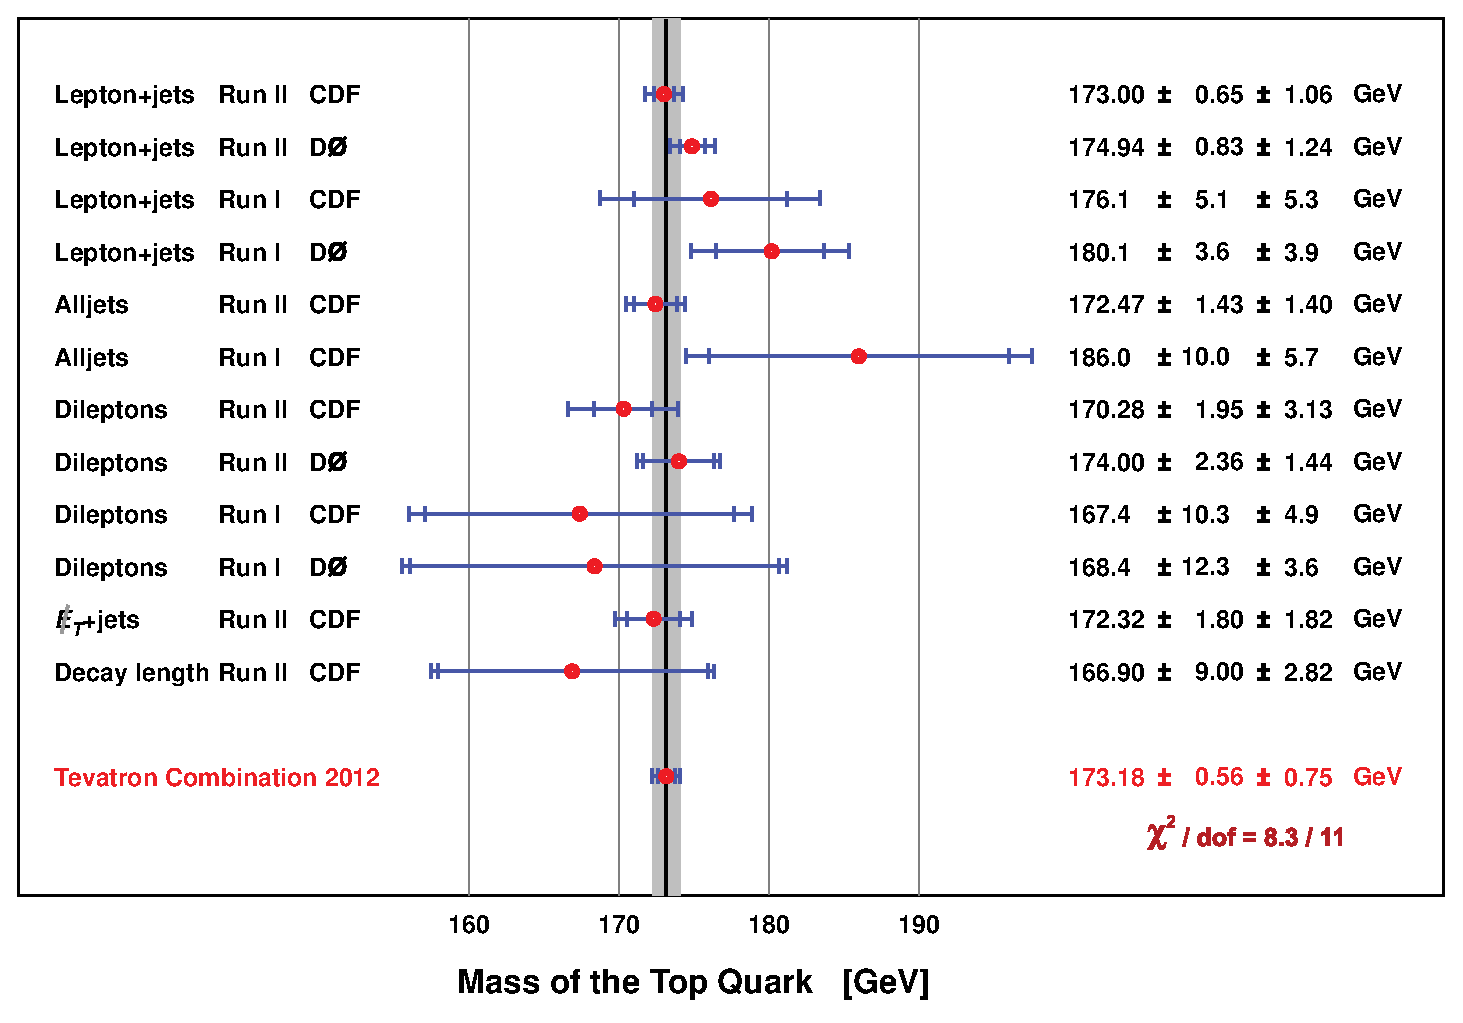
\includegraphics[width=\textwidth]{Figures/Experimental_Results/top_mass_tevatron_2012.eps}
     \caption{Measurement of the top mass from the CDF detector at the Tevatron} \label{fig:topMass_CDF}
   \end{subfigure}
   ~ %add desired spacing between images, e. g. ~, \quad, \qquad, \hfill etc.
      % (or a blank line to force the subfigure onto a new line)
   \begin{subfigure}[h]{0.3\textwidth}
     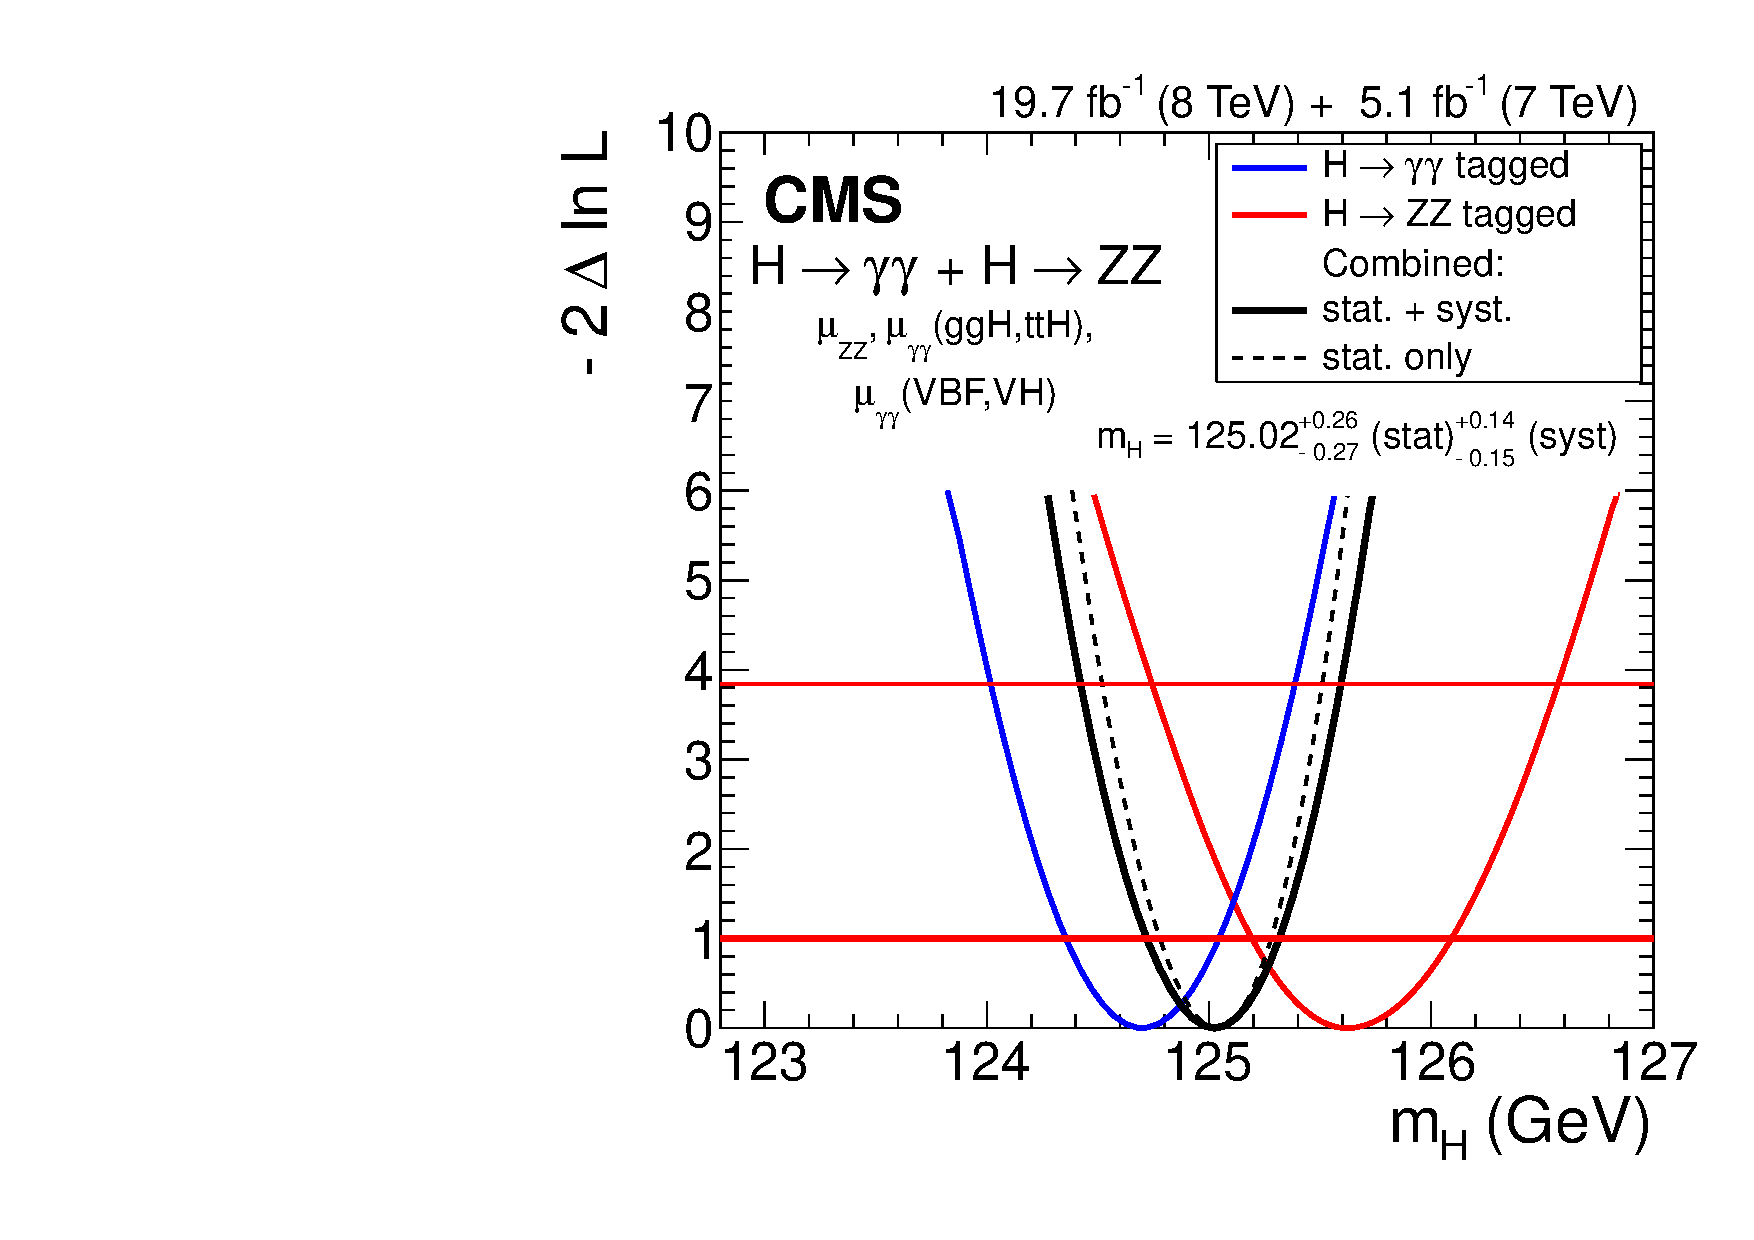
\includegraphics[width=\textwidth]{Figures/Experimental_Results/CMS_higgsMass_scan_1d_all.pdf}
     \caption{Measurement of the Higgs mass from the CMS detector at the LHC} \label{fig:topMass_CDF}
   \end{subfigure}
   \caption{Experimental milestones of the Standard Model}\label{fig:ex_milestones_sm}
\end{figure}

\noindent the experiment was also able to put stringent limits on the
existence of more than three families of leptons and quarks by
measuring the width of the $Z$ boson.  Figure
\ref{fig:ex_milestones_sm}(\subref{fig:lep_Z_3_families}) shows the
comparison of two, three, and four family hypotheses to data.   

\par Another milestone for the Standard Model occured in 1995 when the
CDF~\cite{ex:CDF_topQuark} and D0 experiments~\cite{ex:D0_topQuark} at
the Tevatron announced the observation of the top quark, with
$m_{t}\sim~176~\GeV$, in $p\bar{p}$ collisions at $\sqrt{s}=1.8~\TeV$.
Figure \ref{fig:ex_milestones_sm}(\subref{fig:topMass_CDF}) shows a
plot from 2012, the latest top quark mass measurements from CDF, which
reports a $m_{t} = 173.18 \pm 0.56 \pm 0.75~\GeV$. It was the last
quark predicted by the CKM matrix to be observed, and earned Makoto
Kobayashi and Toshihide Maskawa the nobel prize in 2008 for their work
extending the quark sector to three families and parameterizing their
electroweak mixing.    

\par Yet another milestone was reached in 2012, when the CMS and ATLAS
detectors at CERN anounced the observation of a new boson, with
characteristics strikingly similar to the elusive Higgs boson of the
SM.  Figure \ref{fig:ex_milestones_sm}(\subref{fig:topMass_CDF}) shows
the latest measurement results on the mass from the
$H\rightarrow\gamma\gamma$ and $H\rightarrow~ZZ$ channels, with a
$m_{H} = 125.02 \pm 0.27 \pm 0.15$.  One of the most important
remaining goals is to measure the couplings of this new boson to all
of the other particles in the Standard Model.  Of particular interest
is the coupling to the top-quark, since it offers the largest value of
the Higgs Yukawa coupling to measure.  This offers a test of the
nature of the coupling, as well as a probe into deviations from its
value.   


\section{Higgs Procuction in $pp$ Collisions at the LHC}
\label{higgs_production_overview}

\begin{figure}[h]
   \centering
  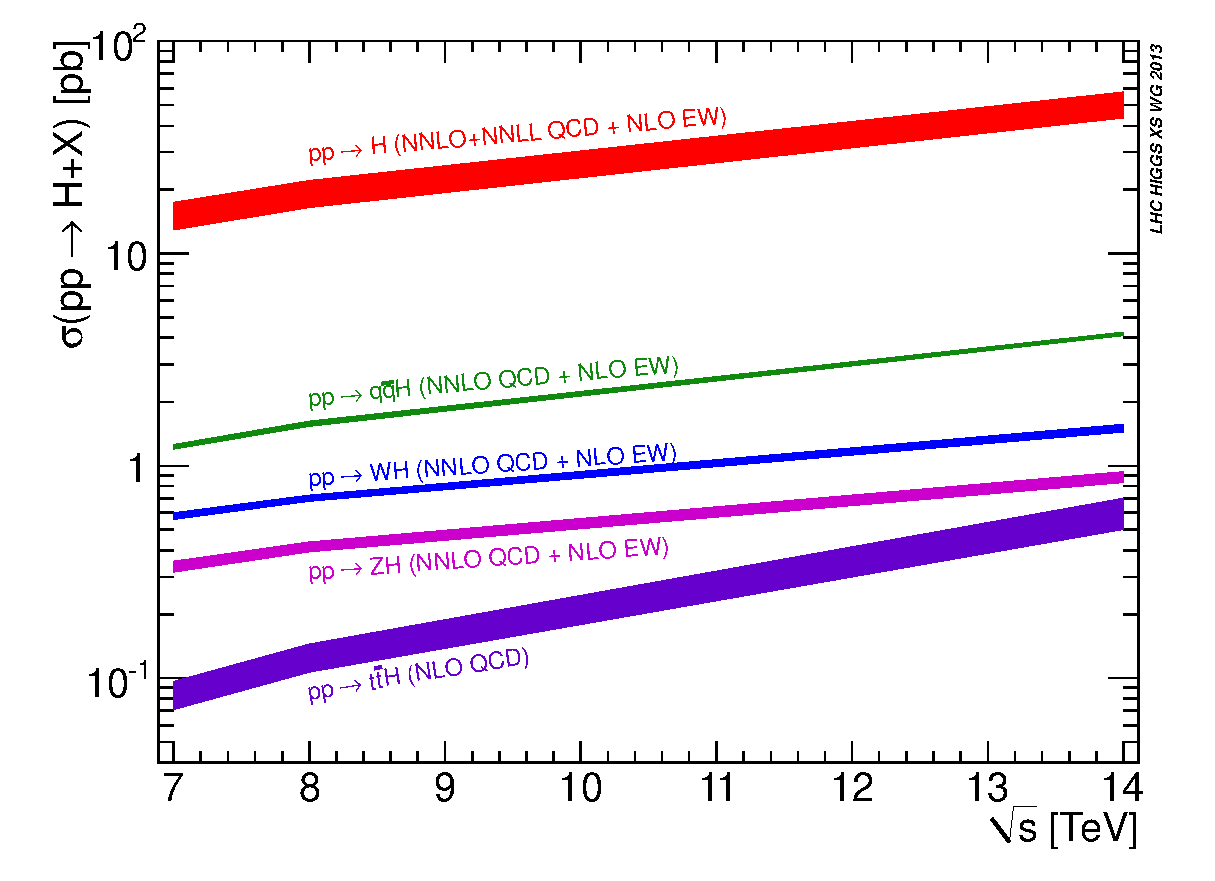
\includegraphics[width=0.5\textwidth]{Figures/Experimental_Results/Higgs_XS_7-14TeV.eps}
  \caption{Higgs production cross-sections at the LHC, for 7-14$\TeV$
    $pp$ collisions} \label{fig:Higgs_XS_7-14TeV}
\end{figure}

\par The rest of the thesis will describe the search for Higgs
boson production in proton-proton collisions at the LHC, so it will be
useful to understand the production mechanisms for the Higgs in this
scenario.  At the LHC collision energies $7-14\TeV$, there are four
dominant production mechanisms that produce Higgs events: gluon-gluon
fusion (ggf), vector-boson fusion (vbf), associated production with
vector bosons (VH), and associated production with top-quark pairs (ttH).  Figure
\ref{fig:Higgs_XS_7-14TeV} shows the relative cross sections for each
of these mechanisms.  

\begin{figure}
    \centering
    \begin{subfigure}[h]{0.3\textwidth}
        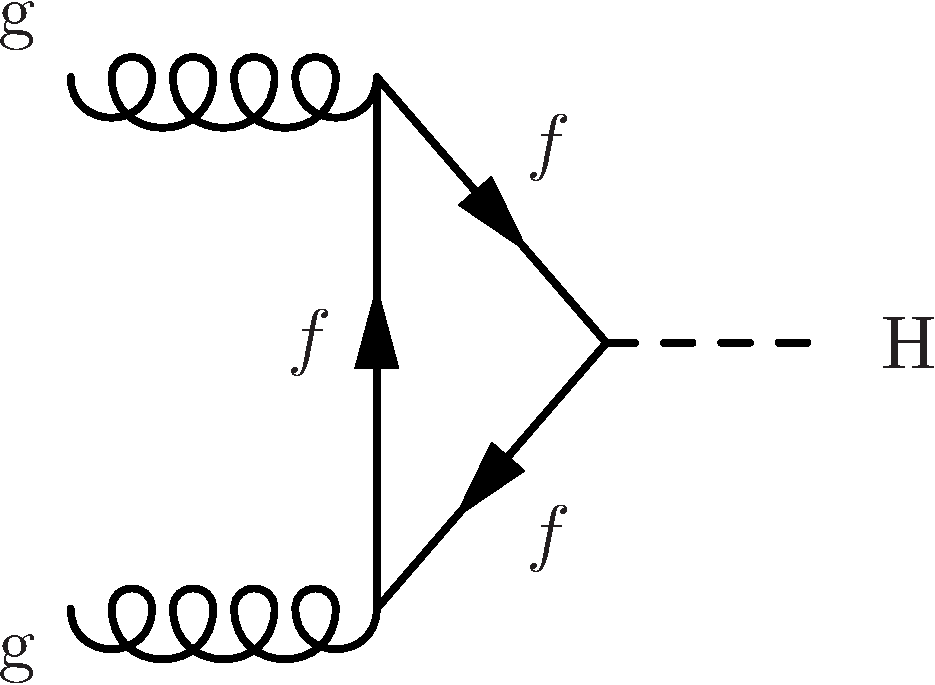
\includegraphics[width=\textwidth]{Figures/Feynman_Diagrams/higgs_production__ggf.pdf}
        \caption{Gluon-Gluon Fusion}\label{fig:higgs_production_ggf}
      \end{subfigure}
      ~ %add desired spacing between images, e. g. ~, \quad, \qquad, \hfill etc.
      % (or a blank line to force the subfigure onto a new line)
      \begin{subfigure}[h]{0.3\textwidth}
        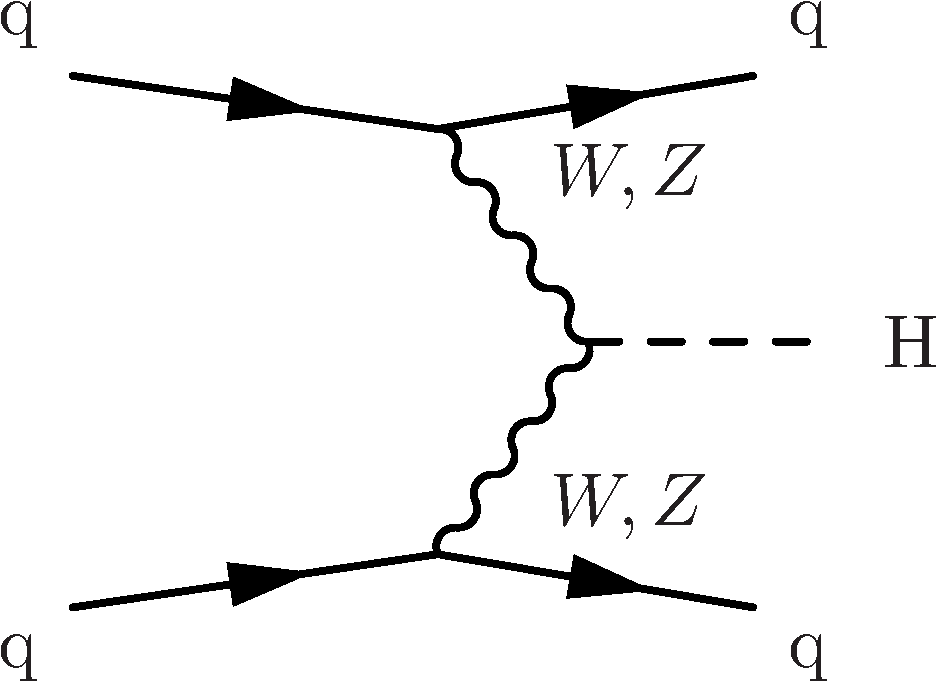
\includegraphics[width=\textwidth]{Figures/Feynman_Diagrams/higgs_production__vbf.pdf}
        \caption{Vector Boson Fusion}\label{fig:higgs_production_vbf}
      \end{subfigure}
      ~ %add desired spacing between images, e. g. ~, \quad, \qquad, \hfill etc.
      % (or a blank line to force the subfigure onto a new line)
      \begin{subfigure}[h]{0.3\textwidth}
        \includegraphics[width=\textwidth]{Figures/Feynman_Diagrams/higgs_production__vh.pdf}
        \caption{Associated Production with $W,Z$}\label{fig:higgs_production_vh}
      \end{subfigure}
      \caption{Feynman diagrams for the three largest Higgs production
        modes at the LHC} \label{fig:feynman_diagrams__higgs_production}
\end{figure}

\par Gluon-gluon fusion, which proceeds via a heavy quark
loop~\cite{th:HiggsXS_2013}, is the dominant production mechanism at
the LHC.  The QCD radiative corrections to the total cross section have been computed
at the next-to-leading order (NLO) and at the next-to-next-to-leading order (NNLO
accuracy).  The cross section for Higgs production at $m_{H} =
125\GeV$ and $\sqrt{s}=8\TeV$, the cross section is given as:
\begin{equation}\label{eq:ggf_xs}
\sigma_{ggF} = 19.27~~\pm \text{~~QCD Scale Unc.}^{+7.2\%}_{-7.8\%}~~\pm
\text{~~PDF+$\alpha_{S}$ Unc.}^{+7.4\%}_{-6.9\%}~~\pbinv
\end{equation}
\noindent Figure \ref{fig:feynman_diagrams__higgs_production}(\subref{fig:higgs_production_ggf}) shows a Feynman
diagram for this process.  The triangle loop contains all strongly
coupled fermions, which is dominated by the top-quark since the
Yukawa coupling to the Higgs is the largest.  

\par Vector boson fusion proceeds through the fusion of $W^{+}W^{-}$
or $Z^{0}Z^{0}$  gauge bosons~\cite{th:HiggsXS_2013}. The
characteristic signature of the production mode is the associated
production of two quarks, typically at a low angle relative to the
proton beam.  This process has been caclulated to NNLO for QCD and NLO
for Electroweak corrections~\cite{th:HiggsXS_2013}.  The cross section
at $m_{H} = 125\GeV$ and $\sqrt{s}=8\TeV$ is given as:
\begin{equation}\label{eq:vbf_xs}
\sigma_{VBF} = 1.653~~\pm \text{~~EW Unc.}^{+4.5\%}_{-4.5\%}~~\pm
\text{~~QCD Scale Unc.}^{+0.2\%}_{-0.2\%}~~\pm
\text{~~PDF+$\alpha_{S}$ Unc.}^{+2.6\%}_{-2.8\%}~~\pbinv 
\end{equation}
\noindent Figure
\ref{fig:feynman_diagrams__higgs_production}(\subref{fig:higgs_production_vbf})
shows a Feynman diagram for VBF production.  The large coupling to the
$W,Z$ bosons helps to make this the sub-dominant production mechanism
at the LHC.  However, the gluon content of the proton at \TeV energies
is much larger than that of the valence quarks, thus the relative
suppression.  

\par The third largest production mechanism for Higgs bosons at the
LHC is through associated production with a $W$ or $Z$
boson~\cite{th:HiggsXS_2013}.  It has been calculated to NNLO for QCD
and NLO for Electroweak corrections. This process is also sometimes
referred to as, Higgstrahlung, since it resemble the bremstrahlung
process of an electron radiating a photon. The higher order
electroweak corrections are similar to that of the Drell-Yan, so much
of the technology to compute the cross-section can be borrowed from
existing EW calculations.  The cross section for $m_{H} = 125\GeV$ and
$\sqrt{s}=8\TeV$ is:  
\begin{equation}\label{eq:vh_xs}
\begin{aligned}
\sigma_{WH} =&~ 0.7046~~\pm \text{~~QCD Scale Unc.}^{+1.0\%}_{-1.0\%}~~\pm
\text{~~PDF+$\alpha_{S}$ Unc.}^{+2.3\%}_{-2.3\%}~~\pbinv \\
\sigma_{ZH} =&~ 0.4153~~\pm \text{~~QCD Scale Unc.}^{+3.1\%}_{-3.1\%}~~\pm
\text{~~PDF+$\alpha_{S}$ Unc.}^{+2.5\%}_{-2.5\%}~~\pbinv 
\end{aligned}
\end{equation}
\noindent Figure
\ref{fig:feynman_diagrams__higgs_production}(\subref{fig:higgs_production_vh})
shows the Feynman diagram for VH production.  This channel is most
useful for identifying hadronic decays of the Higgs, since the
associated gague boson can decay to leptons, giving a strong kinematic
handle over backgrounds that would normally overwhelm a similar search
in the ggF channel.  


\section{\ttH Production in $pp$ Collisions at the LHC}
\label{ttH_production_overview}

\begin{figure}[h]
   \centering
  \includegraphics[width=0.3\textwidth]{Figures/Feynman_Diagrams/higgs_production__ttH.pdf}
  \caption{Feynman diagram for \ttH production} \label{fd:ttH_simple}
\end{figure}

\par The \ttH production mode is the fourth largest production mode at
the LHC~\cite{th:HiggsXS_2013}.  This production mode has been
calculated to NLO in
QCD~\cite{tthXS_NLO_BeenakkerEtAl_1}~\cite{tthXS_NLO_BeenakkerEtAl_2}
and has been studied recently with the state of the art NLO tools
using the aMC@NLO~\cite{tthXS_aMCatNLO_Frederix} and POWHEG
(PYTHIA+HERWIG)~\cite{tthXS_powheg_Garzelli} frameworks. Studies have
also been performed interfacing NLO QCD studies
~\cite{tthXS_NLO_Dawson} with the Sherpa parton shower
framework~\cite{tthXS_sherpa_Gleisberg}.  Additional studies on the
effects of spin correlations with the aMC@NLO and Madspin framework
have also been performed~\cite{tthXS_aMCatNLO_madspin_Artoisenet}.  

\par  It has been found that the additional of NLO effects increases
the cross-section relative to LO by $\sim20\%$.  The largest
theoretical uncertainty comes from the variation of the
renormalization and factorization scale, the QCD coupling $\alpha_{S}$,
and the PDF uncertainty.  The renomarlization and factorization scales
are set to $\mu_{R} = \mu_{F} = (1/2)(m_{T} + m_{T} + m_{H})$ and are
varied by a factor of 2 to determine the cross-section's dependence on
these parameters.  Three different PDF sets,  MSTW2008, CTEQ6.6, and
NNPDF2.0 were used with the appropriate corresponding values of
$\alpha_{S}$ to determine the combined effect of varying
PDF+$\alpha_{S}$.  The cross section for $m_{H} = 125\GeV$ and
$\sqrt{s}=8\TeV$ is given by:
\begin{equation}\label{eq:tth_xs}
\sigma_{ttH} = 0.1293~~\pm \text{~~QCD Scale Unc.}^{+3.8\%}_{-9.3\%}~~\pm
\text{~~PDF+$\alpha_{S}$ Unc.}^{+8.1\%}_{-8.1\%}~~\pbinv
\end{equation}

\noindent A search for the Higgs in this production mode is
additionally challenging due to this large $\sim10\%$ error on the
theoretical cross-section.  Figure \ref{fd:ttH_simple} shows a Feynman
diagram for this process before the branching of the top-quarks or
Higgs to final states.  

\par When asking for the Higgs to decay to b-quark
pairs, yet another complication arrises when trying to identify which
b-quarks came from a top decay or from a Higgs decay.  For example, in
the semileptonic decay of top quarks, there will be four b-quarks, and
two light-flavor quarks in the final state.  This means there are 15
(six choose four) possibilities to associate quarks to the top
system.  Although this is potentially constrained by b-tagging, and
kinematic requirements (such as forming the top or $W$ masses), the
number of remaining possibilites smears out the resolution on peaking
variables such as the invariant mass of b-quark pairs.  


\section{Background Processes to \ttH}
\label{ttH_backgrounds_overview}

\begin{figure}{h}
    \centering
    \begin{subfigure}[h]{0.4\textwidth}
        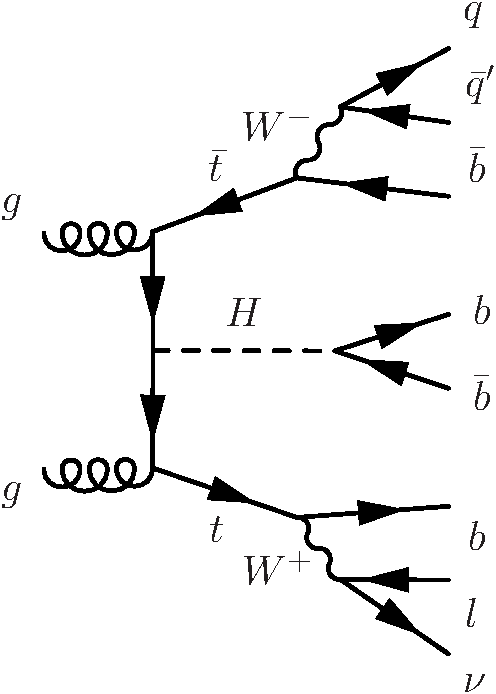
\includegraphics[width=\textwidth]{Figures/Feynman_Diagrams/higgs_production__tth_semileptonic.pdf}
        \caption{Semileptonic \ttH, with $H\rightarrow~b\bar{b}$}\label{fig:higgs_production_tth_semileptonic}
      \end{subfigure}
      ~ %add desired spacing between images, e. g. ~, \quad, \qquad, \hfill etc.
      % (or a blank line to force the subfigure onto a new line)
      \begin{subfigure}[h]{0.4\textwidth}
        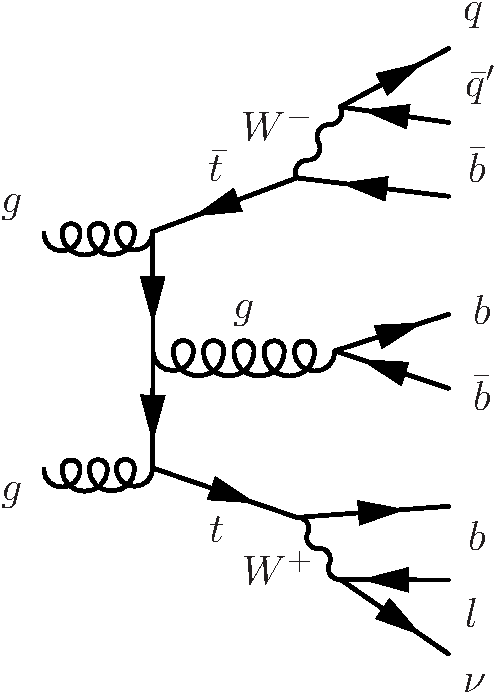
\includegraphics[width=\textwidth]{Figures/Feynman_Diagrams/backgrounds__ttbar_plus_bbar_semileptonic.pdf}
        \caption{Semileptonic \ttbb}\label{fig:higgs_production_vbf}
      \end{subfigure}
      \caption{Feynman diagrams for the semileptonic \ttH process and
        its irreducible background, \ttbb } \label{fig:feynman_diagrams__tth_vs_ttbb_semilep}
\end{figure}

\par The dominant background for \ttH production of top-quark pairs
with additional ISR/FSR jets, \ttjets.  The irreducable component of
this background is comes when the extra radiation produces a final
state with two additional b-quarks, \ttbb.  Figure
\ref{fig:feynman_diagrams__tth_vs_ttbb_semilep} compares the Feyman
diagrams for the semileptonic decays of \ttH and \ttbb.  

\par Additional difficulties come from the theoretical uncertainty on
the \ttbb background~\cite{th:HiggsXS_2013}.  The process has been
calcualted to NLO QCD in Sherpa~\cite{tthXS_sherpa_Gleisberg} and
OpenLoops~\cite{ttbbXS_openloops_Cascioli}~\cite{ttbbXS_openloops_help1_Krauss}~\cite{ttbbXS_openloops_help2_Gleisberg}.
It has been found that depending on selection cuts, and use of NLO PDF
inputs, the difference between LO and NLO calculations on the cross
section can be anywhere from $0.99\%$ to $1.96\%$.  

\par The light flavor component of the \ttjets background also enters
in the selection when any of the jets from the $t\bar{t}$ system or
extra radiation are misidentified as $b$-jets.  The cross-section for
the \ttjets process is $\sim245\pbinv$.  This is a factor of 1800, so
even if a b-tagging algorithm performs with a $1\%$ mis-identification
rate of light-jets, there will still be a large contribution from this
process that will leave a very similar signature in the detector as
\ttH. 

\begin{figure}{h}
    \centering
    \begin{subfigure}[h]{0.4\textwidth}
        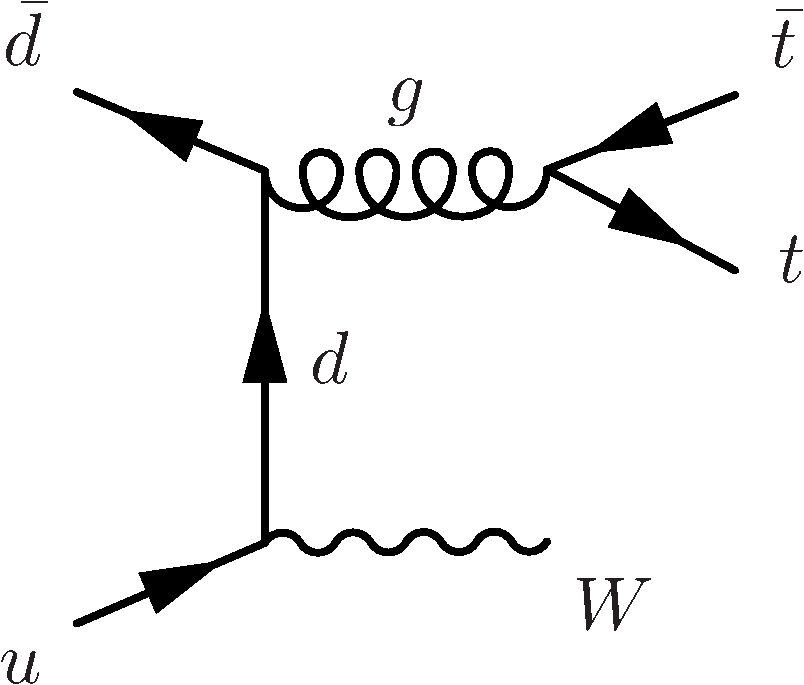
\includegraphics[width=\textwidth]{Figures/Feynman_Diagrams/backgrounds__ttbar_plus_W.pdf}
        \caption{The \ttW background}\label{fd:ttW}
      \end{subfigure}
      ~ %add desired spacing between images, e. g. ~, \quad, \qquad, \hfill etc.
      % (or a blank line to force the subfigure onto a new line)
      \begin{subfigure}[h]{0.4\textwidth}
        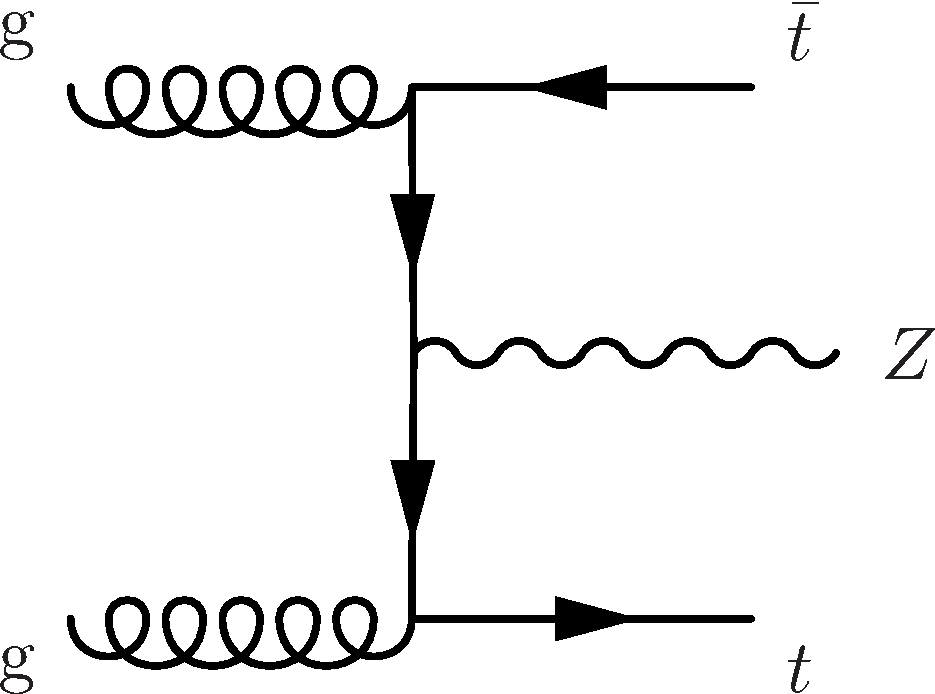
\includegraphics[width=\textwidth]{Figures/Feynman_Diagrams/backgrounds__ttbar_plus_Z.pdf}
        \caption{The \ttZ background}\label{fd:ttZ}
      \end{subfigure}
      \caption{Feynman diagrams for the \ttW and \ttZ background processes} \label{fig:feynman_diagrams__ttW_ttZ}
\end{figure}

\par The next largest background is the production of vector bosons in
association with top-quark pairs, \ttW and \ttZ.  Figure
\ref{fig:feynman_diagrams__ttW_ttZ} shows Feynman diagrams from these
two processes.  They have cross-sections of $\sigma_{ttW}=0.249\pbinv$
and $\sigma_{ttZ}=0.208\pbinv$, which are only a factor of $\sim$2
greater than the \ttH process.  These processes can enter the
semileptonic \ttH selection by a semileptonic \ttbar decay, while the
vector bosons decay to quarks, or through a hadronic \ttbar decay,
while the vector bosons decay to quarks, and in the case of \ttZ, of
the leptons is not identified in the reconstruction.  

\begin{figure}{h}
    \centering
    \begin{subfigure}[h]{0.3\textwidth}
        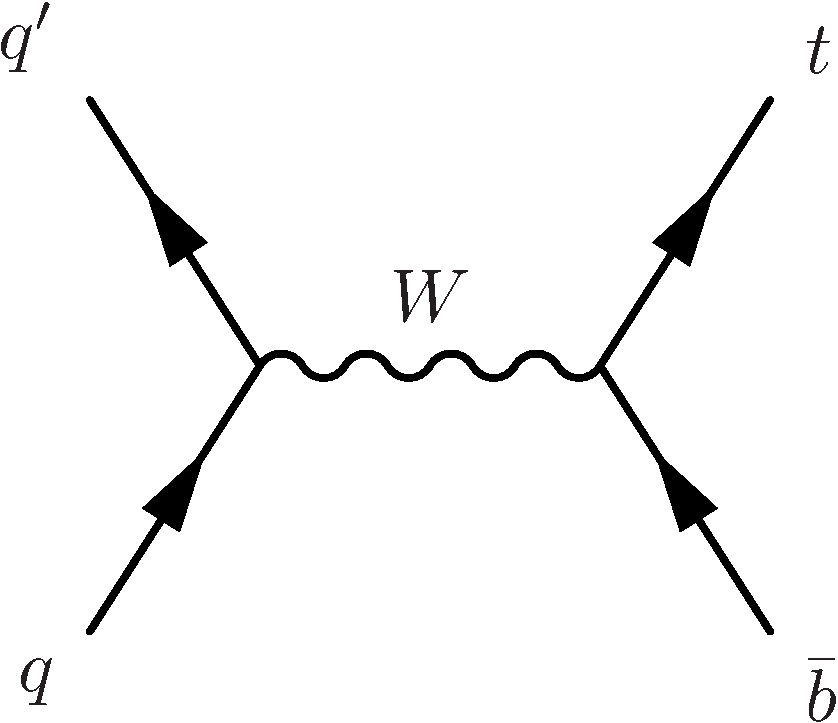
\includegraphics[width=\textwidth]{Figures/Feynman_Diagrams/backgrounds_singleT_sChan.pdf}
        \caption{Single $t$, s-channel}\label{fd:t_sChan}
      \end{subfigure}
      ~ %add desired spacing between images, e. g. ~, \quad, \qquad, \hfill etc.
      % (or a blank line to force the subfigure onto a new line)
      \begin{subfigure}[h]{0.3\textwidth}
        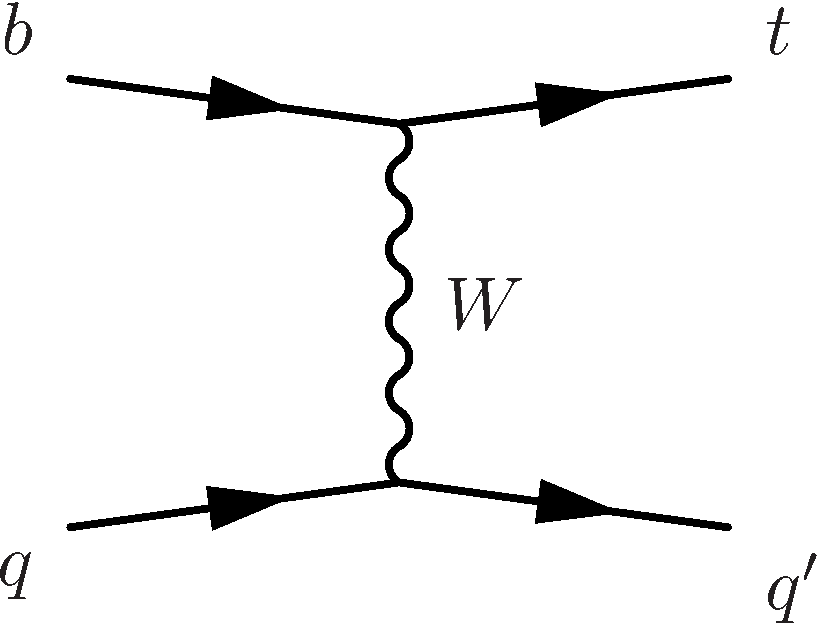
\includegraphics[width=\textwidth]{Figures/Feynman_Diagrams/backgrounds_singleT_tChan.pdf}
        \caption{Single $t$, t-channel}\label{fd:t_tChan}
      \end{subfigure}
      ~ %add desired spacing between images, e. g. ~, \quad, \qquad, \hfill etc.
      % (or a blank line to force the subfigure onto a new line)
      \begin{subfigure}[h]{0.3\textwidth}
        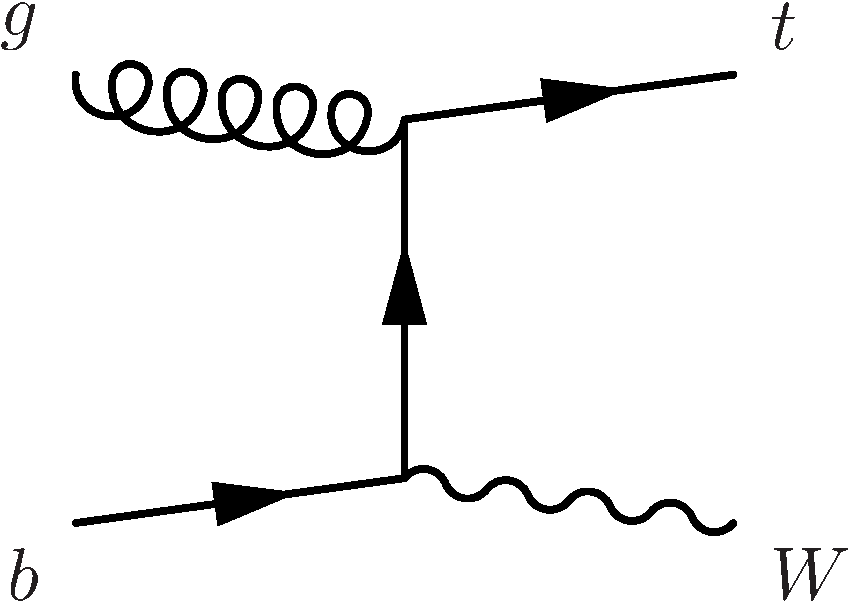
\includegraphics[width=\textwidth]{Figures/Feynman_Diagrams/backgrounds_singleT_tWChan.pdf}
        \caption{Single $t$, tW-channel}\label{fd:t_tWChan}
      \end{subfigure}
      \caption{Feynman diagrams for the single $t$ s,t, and t$W$ background processes} \label{fig:feynman_diagrams__singleT_t_s_tW_channels}
\end{figure}


\par Single top production is also an important background to consider
in a search for \ttH production.  Figure
\ref{fig:feynman_diagrams__singleT_t_s_tW_channels} shows Feynman
diagrams for this process.  It does not have as large of a
contribution as the other backgrounds, since it requires addional
radiation in order to have a similar final state jet multiplicity as
\ttH.  However, since a top-quark is still involved in the process,
the final state kinematics of its decay products will be very similar.
 Single $t$ production has a cross section of $\sigma_{t}=71.3\pbinv$,
 while Single $\bar{t}$ production has a cross section of
 $\sigma_{\bar{t}}=43.6\pbinv$, due to charge asymmetry of the valence
 quarks of the proton

\begin{figure}{h}
    \centering
    \begin{subfigure}[h]{0.3\textwidth}
        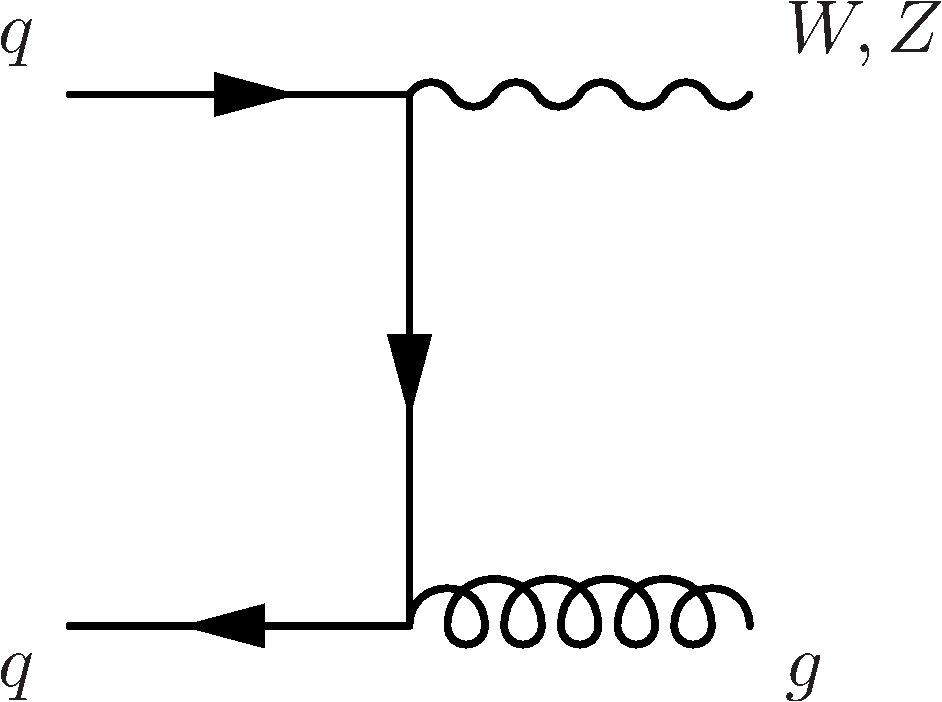
\includegraphics[width=\textwidth]{Figures/Feynman_Diagrams/backgrounds__VplusJets.pdf}
        \caption{$W,Z$ plus jets}\label{fd:t_tChan}
      \end{subfigure}
      ~ %add desired spacing between images, e. g. ~, \quad, \qquad, \hfill etc.
      % (or a blank line to force the subfigure onto a new line)
      \begin{subfigure}[h]{0.3\textwidth}
        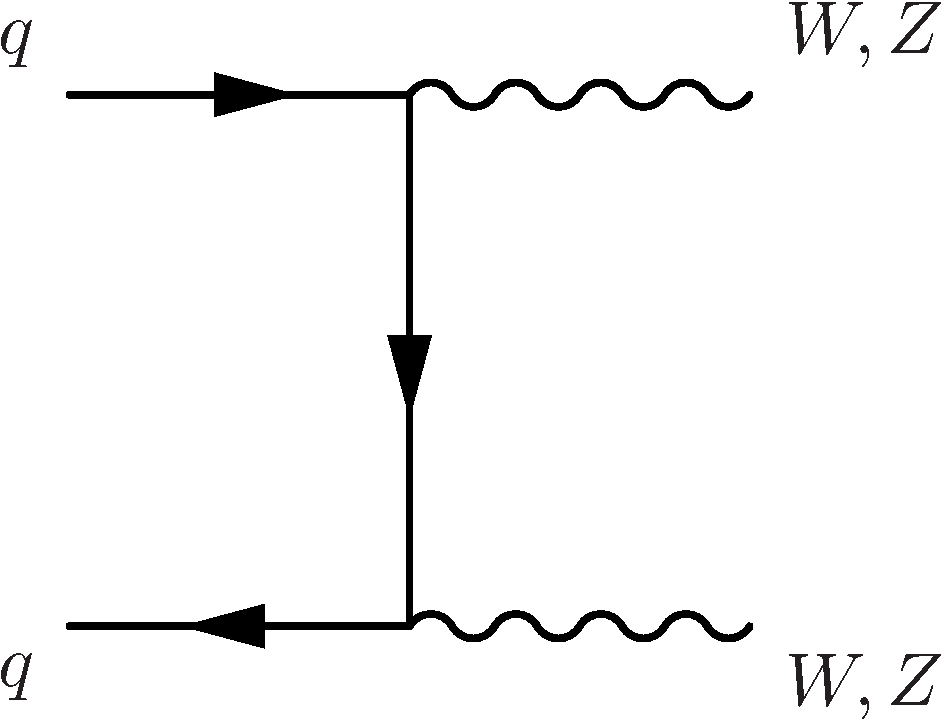
\includegraphics[width=\textwidth]{Figures/Feynman_Diagrams/backgrounds__VV.pdf}
        \caption{DiBoson Production}\label{fd:VV}
      \end{subfigure}
      \caption{Feynman diagrams for the $W,Z$ plus jets, and diBoson
        ($WW$, $WZ$, $ZZ$) production.} \label{fig:feynman_diagrams__Vjets__VV}
\end{figure}

\par The last backgorunds to consider are the electroweak production
of $W$ and $Z$ bosons in association with jets, as well as $WW$, $WZ$, and
$ZZ$ pairs in association with jets.  Figure
\ref{fig:feynman_diagrams__Vjets_VV} shows the Feynman diagrams for
these processes, where the $V$, stands in for wither $W$ or $Z$
bosons.  For a semileptonic selection of \ttH events, $Z$ plus jets
events enter from a mis-identification of one of the leptons from the
$Z$ boson decay.  Extra FSR/ISR radiation is also to leave a similar
signature in the signal region of a \ttH search, so it mainly
contributes to control regions of the data.  

\section{Potential BSM Effects on~\ttH~production}
\label{bsm_effects_overview}

\par The phenomological motivation for the existence of physics beyond
the Standard Model come from the observation of phenomenon or states
of matter not described by the theory.  Observations of the cosmic miscrowave background
from the Plank telescope have estimated that only $\sim5\%$ of the
observable universe is composed of ordinary
matter~\cite{BSM_Planck}. The remaining composition is divided between  
Dark Matter ($\sim27\%$, and $\sim68\%$ respecitvely).  Evidence for
Dark Matter also comes from discrepencies between the observed
rotational velocities of galaxies, and the observed mass
distributions, suggesting the presence of additional form of matter
which does not interact
electromagnetically~\cite{BSM_Rubin_DM_GalaxyRotations}.

\par Additionally, in 1998, the Super-Kamiokande experiment proved that
neutrinos oscillated between flavors, implying indirectly that they
also have mass~\cite{BSM_superK}.  This is something not described in
the Standard Model of physics.  Due to their neutral charge, these
particles  are extremely difficult to detect, so experiments have only
been able to measure differences in the mass squared between the three
mass eigenstates.  In 2005, the KamLAND experiment reported
$|{\Delta}m^{2}_{12}=0.000079
eV^{2}|$~\cite{BSM_neutrinoDeltaM12_kamland}.  In 2006, the MINOS
experiment reported
$|{\Delta}m_{23}=0.0027 eV^{2}|$~\cite{BSM_neutrinoDeltaM23_minos}.

\par One of the largest theoretical problems with the Standard Model,
comes the mechanism which made it all possible- the Higgs.  In
equation \ref{eq:ewk_lagrangian_unbroken} there are terms that couple
the Higgs boson to itself, $-{\lambda}vh^{3}$, and
$-\frac{1}{4}{\lambda}h^{4}$.  When computing NLO effects, these terms
lead to a divergence in the Higgs mass, when considering the effect of
a loop of fermions on the Higgs propagator.  The correctios are of the form ${\Delta}m_{H} =
-\frac{\lambda_{f}^{2}}{8\pi^{2}}\Lambda_{UV}$.  Where $\Lambda_{UV}$
is the high energy cut off for the theory, which in the limit of a
perfect theory, should extend to infinity.  This is known as the
hierarchy problem.  

\par Beyond the Standard Model physics is a term that describes
extensions of the Standard Model in order to describe the observed
phenomenon.  For the neutrino oscilations, a solution similar to CKM
matrix has been proposed, the Pontecorvo–Maki–Nakagawa–Sakata (PMNS)
matrix.  This proposes that the mass eigenstates of the neutrino are
linear combinations of the weak eigenstates, allowing for the mixing
of flavors.  Current experiments now seek to measure the free
parameters of this matrix.  

\begin{figure}[h]
   \centering
  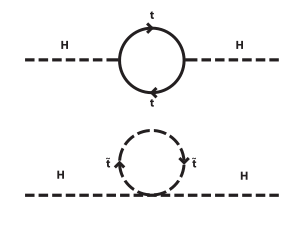
\includegraphics[width=0.5\textwidth]{Figures/Basic_Diagrams/hierarchy_problem_susy_solution.png}
  \caption{The cancellation of the divergent Higgs mass from a loop of
  top-quarks is cancelled by a loop of supersymmetric top-quarks,
  stop-quarks,} \label{fig:hierarchy_problem}
\end{figure}

\par Both the dark matter and hierarchy problems suffer in the fact
that there is no clear model, such as the PMNS matrix, to provide a
theoretical solution.  Out of the plethora of theories that attempt to
solve these problems, supersymmetry (SUSY) is the most popular in the
theoretical and experimental community.  It suggests that there is a
broken symmetry between fermions and bosons, and introduces a partner
to each Standard Model particle with a spin quantum number less
1/2~\cite{Martin_SUSY_primer}.  For the hierarch problem, this
provides a set of particles to cancel out the divergences in the NLO
corrections to the Higgs mass.  Figure \ref{fig:hierarchy_problem}
shows the Feynmann diagrams for a supersymmetric top-quark, or stop
quark, that would cancel the divergent contribution from the Standard
Model top quark.  Depending on the specific form of the SUSY model,
the stop quarks can potentially couple directly or indirectly to the
top-quark, producing them at a higer rate during $pp$ collisions.
This would effect the number of observed events making it into the
\ttH~selection.  

\par A number of extensions to the SM also involve introducing new
top-like particles into the theory.  Vector-like quarks would be spin
1/2 particles that transform as triplets under the $SU(3)$ color group
and whose left and right-handed components have the same  
color and electroweak quantum
numbers~\cite{VectorLikeQuarks_Aguilar-Saavedra}.  These objects are
common to several different types of models.  Little Higgs
models~\cite{BSM_littleHiggs_Burdman}~\cite{BSM_littleHiggs_Perelstein}~\cite{BSM_littleHiggs_PhysRevD.74.055001}, 
models with extra
dimensions~\cite{BSM_extraD_Cheng:1999bg}~\cite{BSM_extraD_Carena:2006bn},
top-color models~\cite{BSM_topColor_Hill:1991at}, and composite Higgs
models~\cite{BSM_composite_Higgs_Contino:2006qr}, include a
vector-like top partner,$ t^{\prime}$ that decays to a top-quark and
either a Higgs, $W$, or $Z$ particle.  Both $t^{\prime}t^{\prime}$
pair production and $t^{\prime}t$ production would yield the ttH final
state, or at least one indistinguishable detector signature.  \ttH
search can provide indirect limits on these models, by observing an
excess or lack thereof of \ttH events, without having to directly
construct a $t^{\prime}$ resonance.  


      

\chapter{The Large Hadron Collider}
\label{lhc_overview}

\begin{figure}[h]
   \centering
  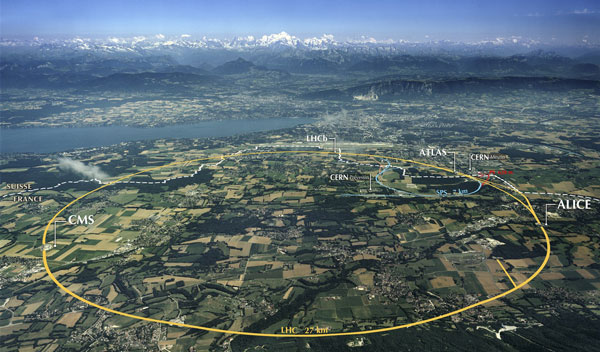
\includegraphics[width=1.0\textwidth]{Figures/LHC_Diagrams/LHC_Aerial_View.jpg}
  \caption{Aerial view of the LHC complex, spanning the French-Swiss border~\cite{LHC:Aerial_View}} \label{fig:lhc_aerial_with_labels}
\end{figure}

\par The \acrfull{lhc}, is a superconducting, proton-proton,
accelerator and collider operated by the \acrfull{cern} laboratory in
Geneva, Switzerland~\cite{lhc:machine_description}.  Figure
\ref{fig:lhc_aerial_with_labels} shows an aerial view of the LHC
complex, with the main laboratory camus being labeled as CERN, with
four of the detector experiments being labeled as ALICE, ATLAS, CMS,
and LHCb.  Three smaller experiments, not pictured, also use the LHC
ring, and are TOTEM, LHCf, and MOeDAL.  It was designed to elucidate
the mechanism of electroweak symmetry breaking and explore \TeV scale
of particle physics.  As such, it is required to produce a large
number of high center-of-mass energy events.  The high center-of-mass
energy allows the creation of heavy particles, while a large
luminosity allows for the creation of rare processes.  The number of events
produced at a collider is a product of the luminosity of the collider
and the total cross-section for the objects being collided.  

\begin{equation}\label{eq:Nevents}
N_{events} = L\sigma_{event}
\end{equation}

\noindent  The cross-section, $\sigma_{event}$, can be estimated from the
theory of the Standard Model as described in section
\ref{qft_overview} and validated by measuremnt at detectors, such as
CMS, as shown in section \ref{ttH_backgrounds_overview}.  The
luminosity is a control of the experiment, and for Guassian
distributed beams, is given by the equation:

\begin{equation}\label{eq:lumi}
L = \frac{ N_{b}^{2}n_{b}f_{rev}\gamma_{r}
}{ 4\pi\epsilon_{n}\beta^{\ast} }F
\end{equation}

\noindent The parameters of this equation and their value for the LHC
is as follows:
\begin{itemize}
\item $N_{b}$ - Number of of particles per bunch, squared since there
  are two beams.  The mechanism of acheiving such high energies is
  based in Radio-Frequency (RF) cavity technology, which clusters the
  protons together into packets, which are all accelerated and
  collided together.  For the LHC, $N_{b} = 1.15 x 10^{11}$.
\item $n_{b}$ - Number of bunches per beam.  The maximum design for
  the LHC allows for $n_{b} = 2808$ bunches, however in practice,
  lower number of bunches have been run with in order to create more
  time between bunch crossings.  
\item $f_{rev}$ - Revolution frequency of the protons in the LHC
  ring.  This is determined by ring circumference, and for the LHC,
  $f_{rev} = 11.2$ kHz. 
\item $\gamma_{r}$ - This is the relativistic gamma-factor, determined
  by the speed, and thus the center of mass energy of the collisions.  
\item $\epsilon_{n}$ - This is the normalized transverse emmitance of
  the beam, which describes the RMS spread of the beam in its
  transverse plane.  For the LHC $\epsilon_{n} = 3.75~\mu$m.  
\item $\beta^{\ast}$ - Is the minimum of the $\beta$ function, which
  is defined as the square of the transverse beamsize divided by
  $\epsilon_{n}$.  It is minimized at interaction regions, where the
  beams are being squeezed into the smallest region possible, to
  maximize the probability of protons colliding during each bunch
  crossing.  For the LHC, $\beta^{\ast} = 0.55$ 
\item $F$ - This is the efficiency for having the two beams head-on,
  and is determined by the crossing angle at which the two
  counter-rotating beams meet each other.  
\end{itemize}

\noindent The LHC is designed to deliver a maximum luminosity of L =
10$^{34}$cm$^{2}$s$^{1}$ to the CMS and ATLAS experiments, with a
maximum center-of-mass energy of $\sqrt{s}=14\TeV$.  


\begin{figure}[h]
   \centering
  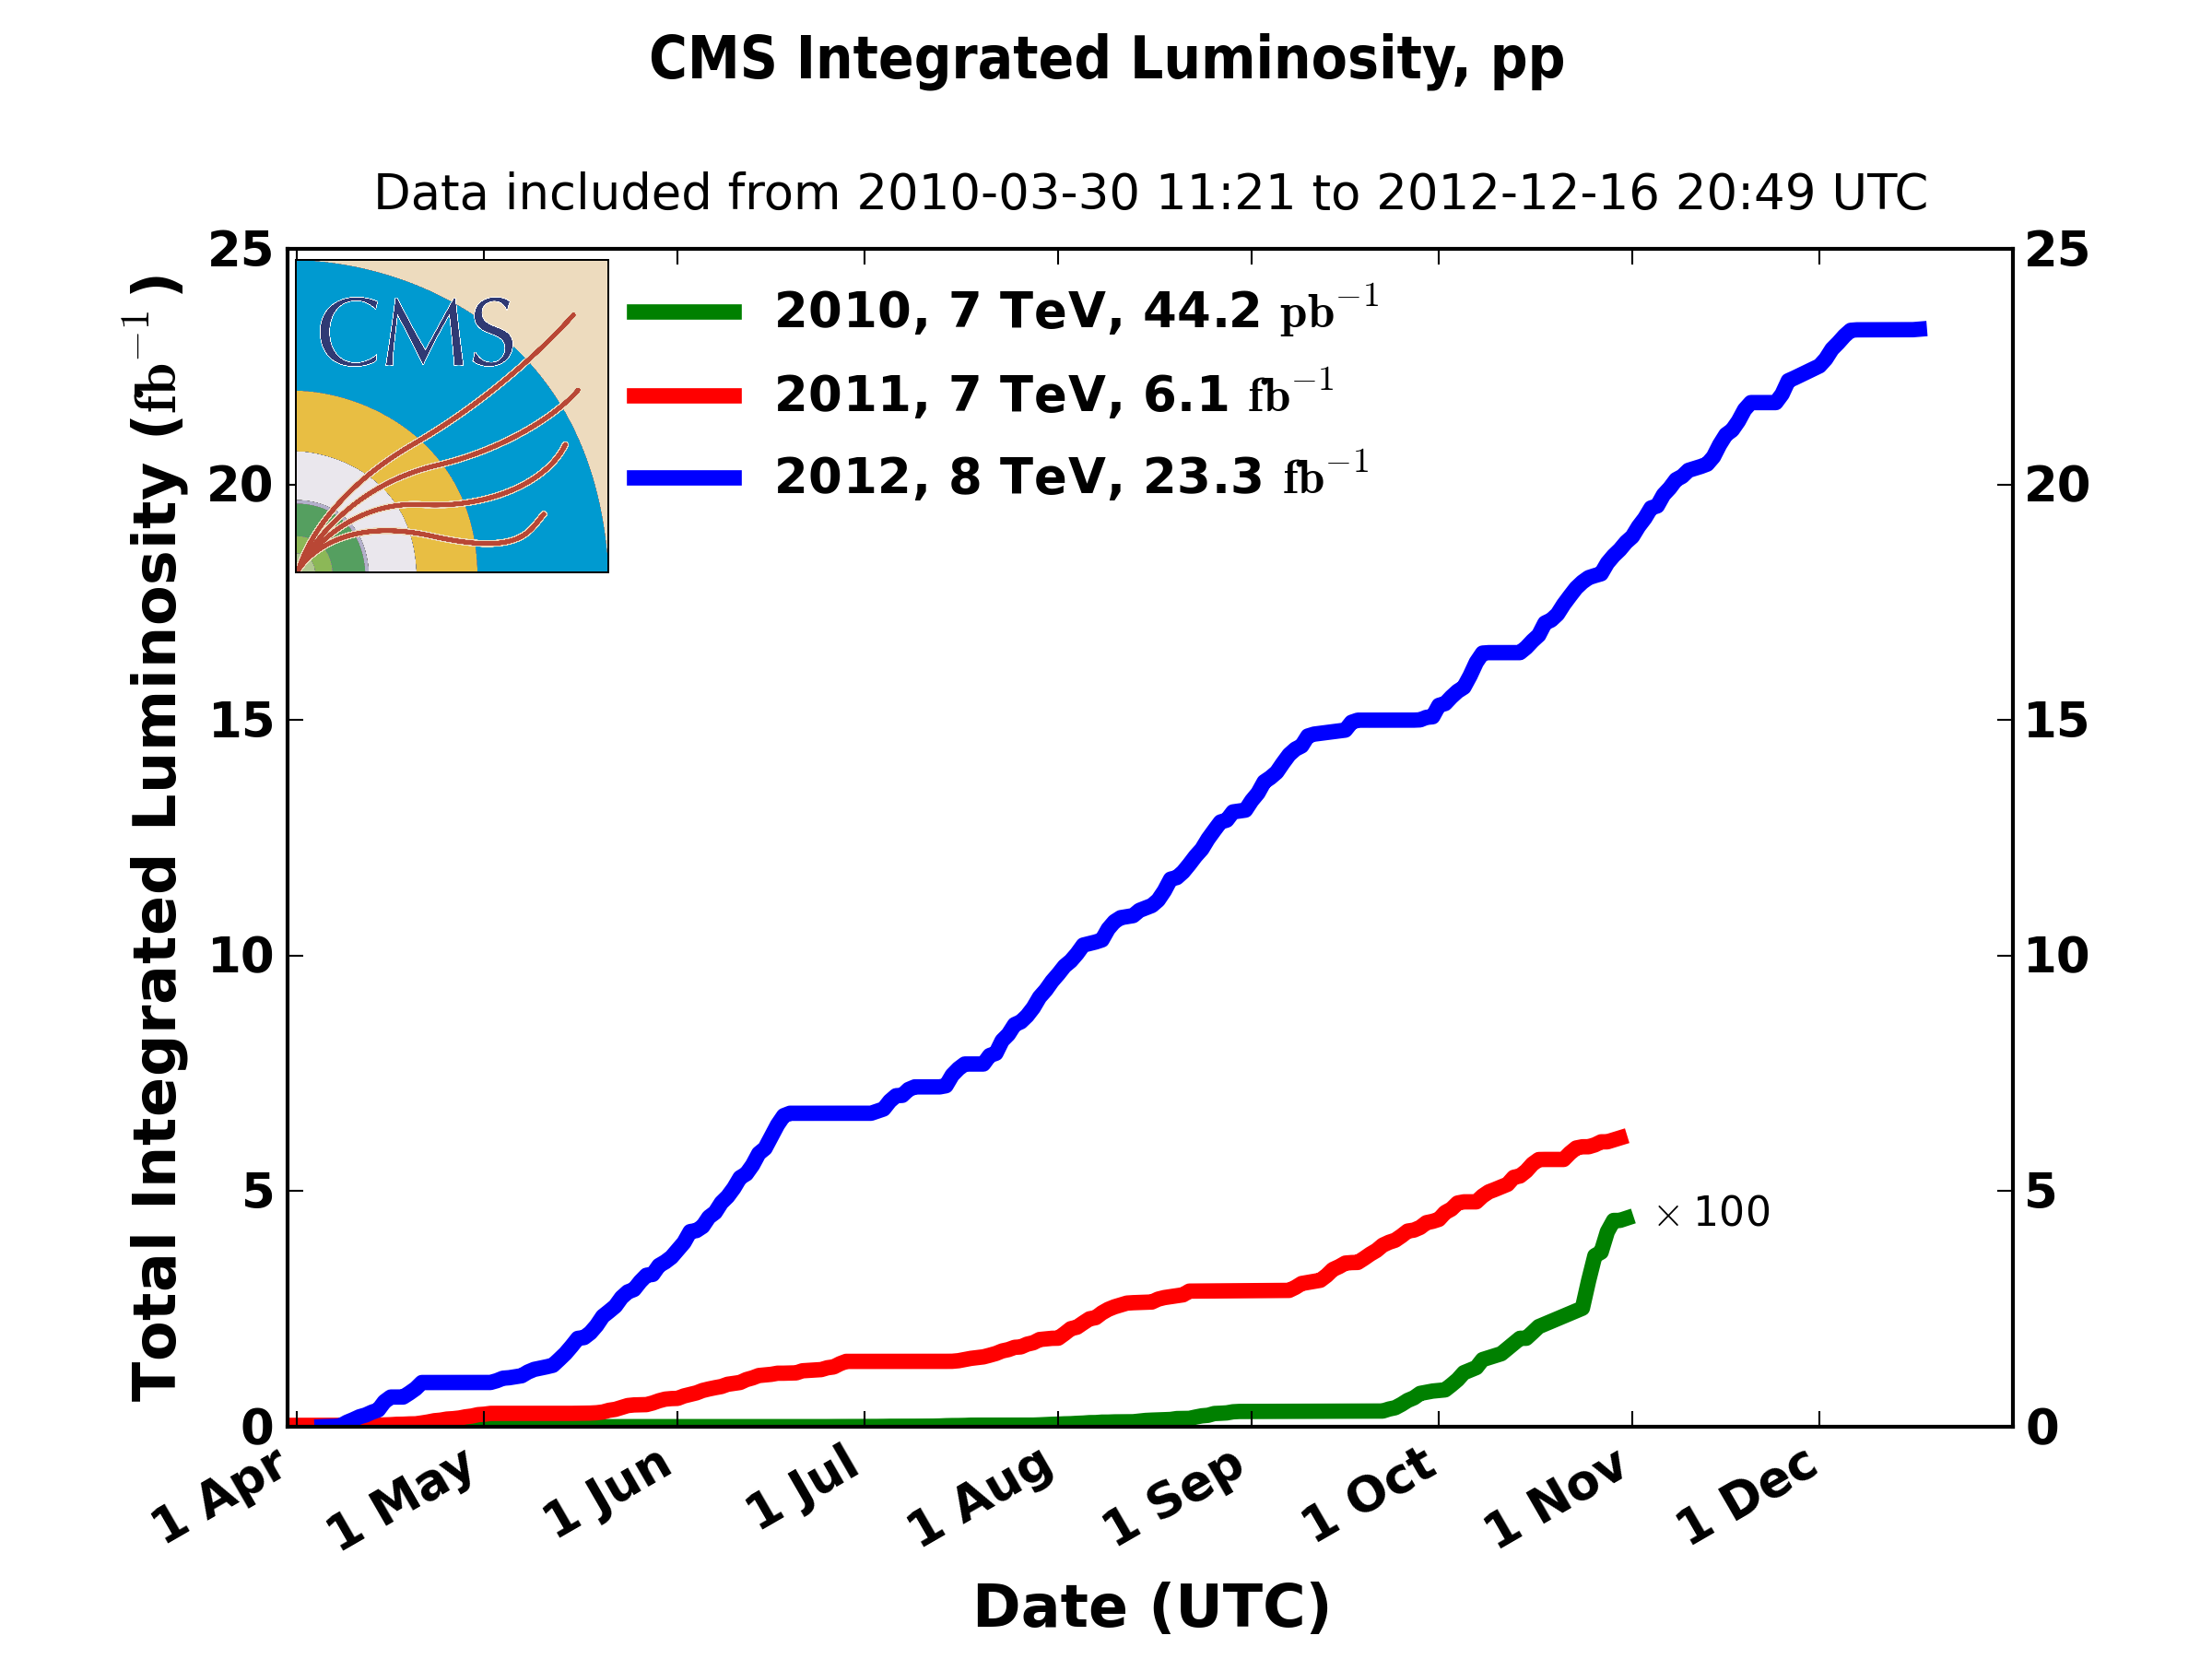
\includegraphics[width=0.8\textwidth]{Figures/Experimental_Results/CMS__int_lumi_cumulative_pp_2.png}
  \caption{Integrated Luminosity delived to the CMS experiment from 2010-12} \label{fig:cms_integrated_lumi}
\end{figure}

\par In 2010-11, the LHC ran at center-of-mass energy,
$\sqrt{s}=7\TeV$ and delivered $\sim6\fbinv$ of data to the CMS
experiment.  In 2012, it ran at $\sqrt{s}=8\TeV$ and collected
$\sim23\fbinv$.  Figure \ref{fig:cms_integrated_lumi} shows a diagram of
the luminosity collected as a function of time for each year running.  

\par The next sections will describe the LHC accelerator complex, the
chain of events leading up to collisions of protons at the LHC, and
the associated technologies that allow for the control and operation
of the high-energy, high-luminosity beams that allow the CMS and ATLAS
experiments to search for heavy particles and rare-processes.  


\section{The LHC Accelerator Complex}
\label{lhc_injection_chain}

\par The main LHC ring is a 26.7 km tunnel, that is 45 m to 170 m
underneath the surface of the earth, with 1.4$\%$ slope towards Lake
Leman.  It extends accross the French-Swiss border, into the French
coutnryside.  The tunnel was originally constructed between 1984 and 1989 for
the Large Electron Positron (LEP) experiment that is famous for it's
precision mesaurements of several Standard Model
parameters~\cite{lhc:machine_description}.  The choice to build the
ring underground was driven by real estate costs, but the underground
setting also provides natural radiation shielding from the beamline
and greatly reduces the impact of cosmic radiation on the detectors.  

\begin{figure}[h]
   \centering
  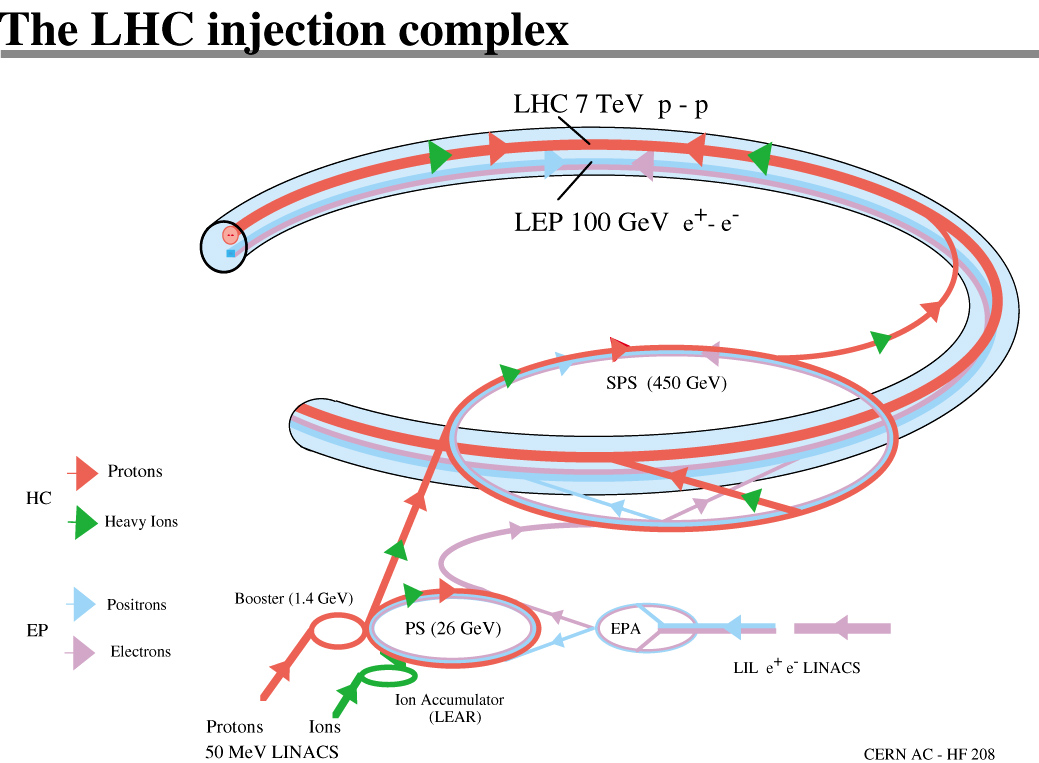
\includegraphics[width=0.8\textwidth]{Figures/LHC_Diagrams/LHC_injection_complex.jpg}
  \caption{The LHC accelerator complex, taking protons from a bottle
    of Hydrogen at the Linac2, all the way to the LHC
    ring} \label{fig:lhc_accelerator_complex}
\end{figure}

\par The LHC also utilizes the existing accelerator complex from the
LEP expermiment, which is shown in figure
\ref{fig:lhc_accelerator_complex}.  The complex is composed a series
of increasingly powerful accelerators that gradually increase the
energy of the protons.  

\begin{figure}{h}
    \centering
    \begin{subfigure}[h]{0.4\textwidth}
        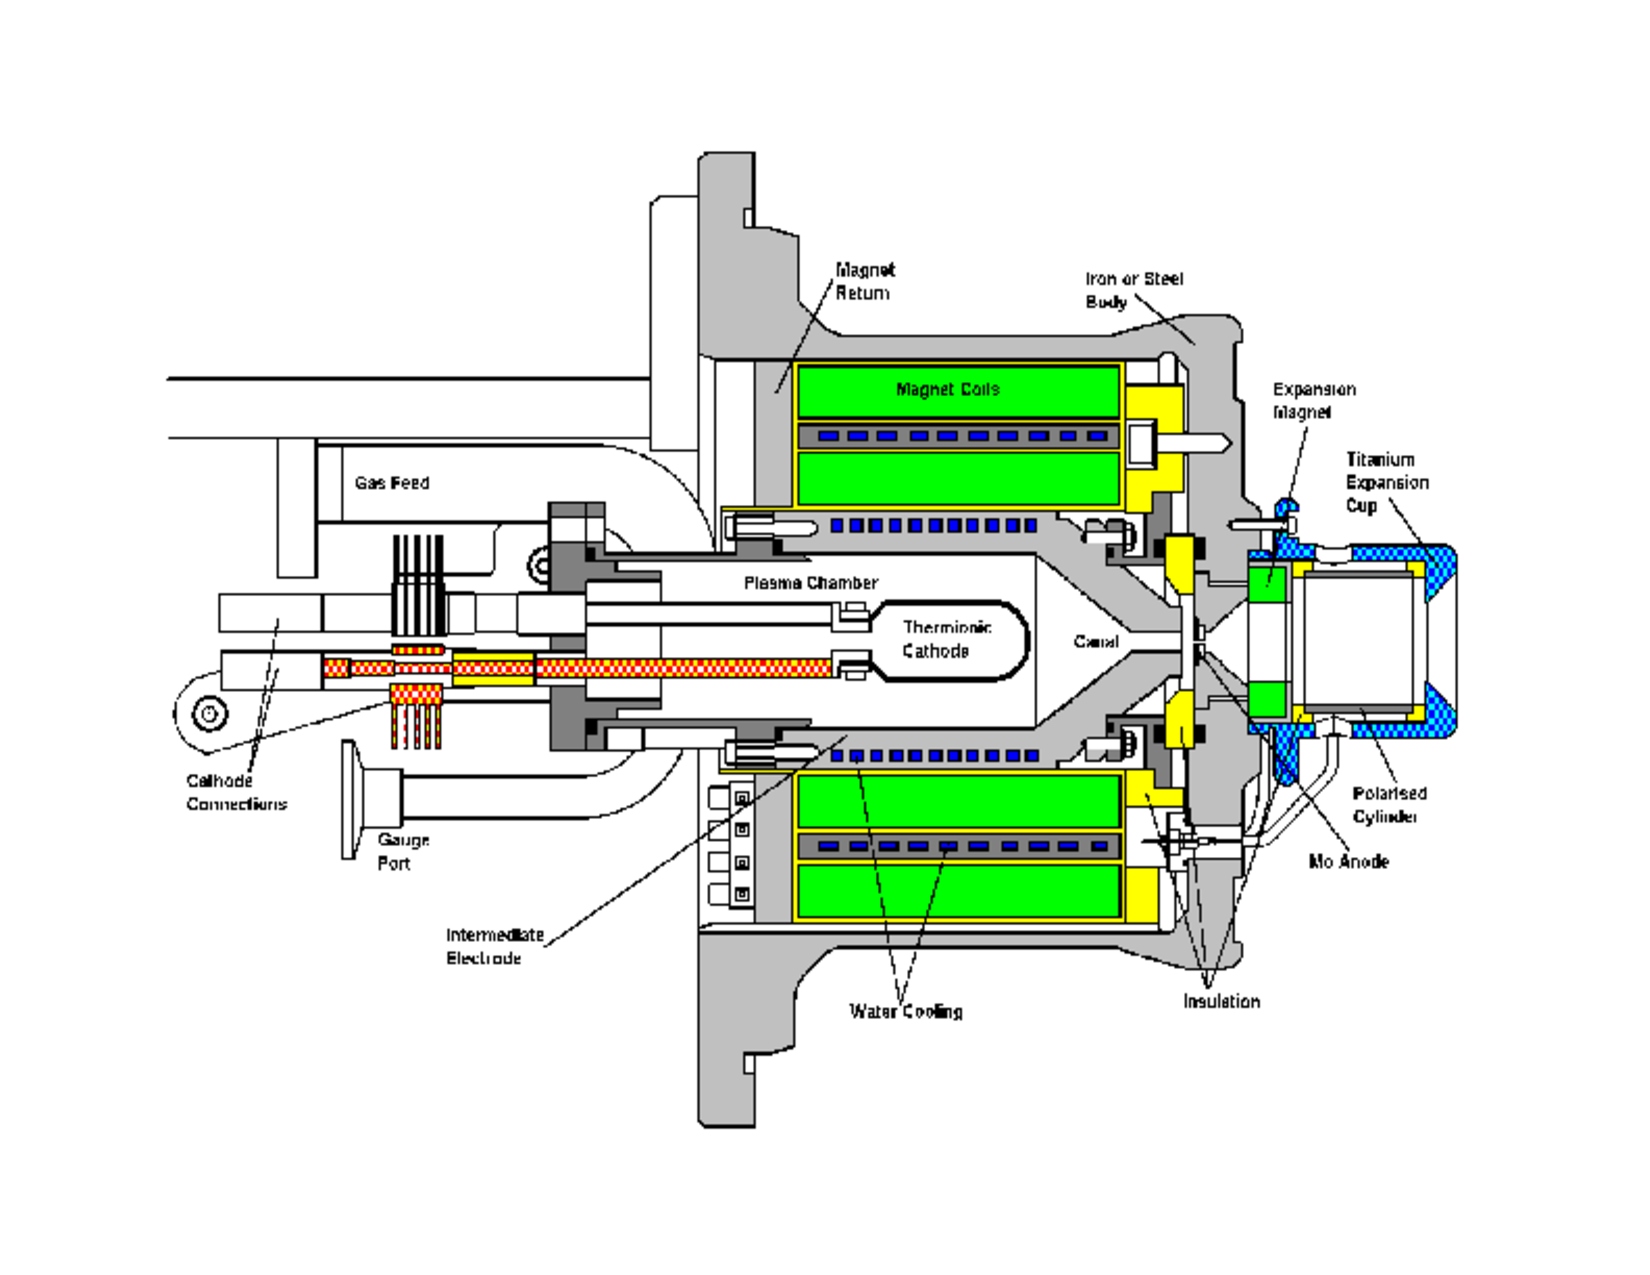
\includegraphics[width=\textwidth]{Figures/LHC_Diagrams/LHC__Linac2__Duoplasmatron_Schematic.pdf}
        \caption{Schematic of the duoplasmatron ion source, which
          creates a proton beam from source bottle of Hyrdogen}\label{fig:duoplasmatron_schematic}
      \end{subfigure}
      ~ %add desired spacing between images, e. g. ~, \quad, \qquad, \hfill etc.
      % (or a blank line to force the subfigure onto a new line)
      \begin{subfigure}[h]{0.4\textwidth}
        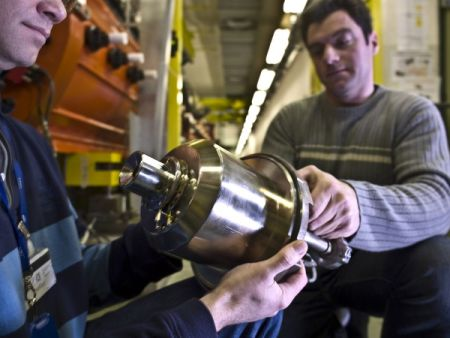
\includegraphics[width=\textwidth]{Figures/LHC_Diagrams/LHC__Linac2__Duoplasmatron__CF002521-ProtonSourceDuoplasmatronRichardChristianss.jpg}
        \caption{The Duoplasmatron used in the Linac2 at CERN, the
          source of the LHC proton beam}\label{fig:duoplasmatron_actual}
      \end{subfigure}
       ~ %add desired spacing between images, e. g. ~, \quad, \qquad, \hfill etc.
      % (or a blank line to force the subfigure onto a new line)
      \begin{subfigure}[h]{0.4\textwidth}
        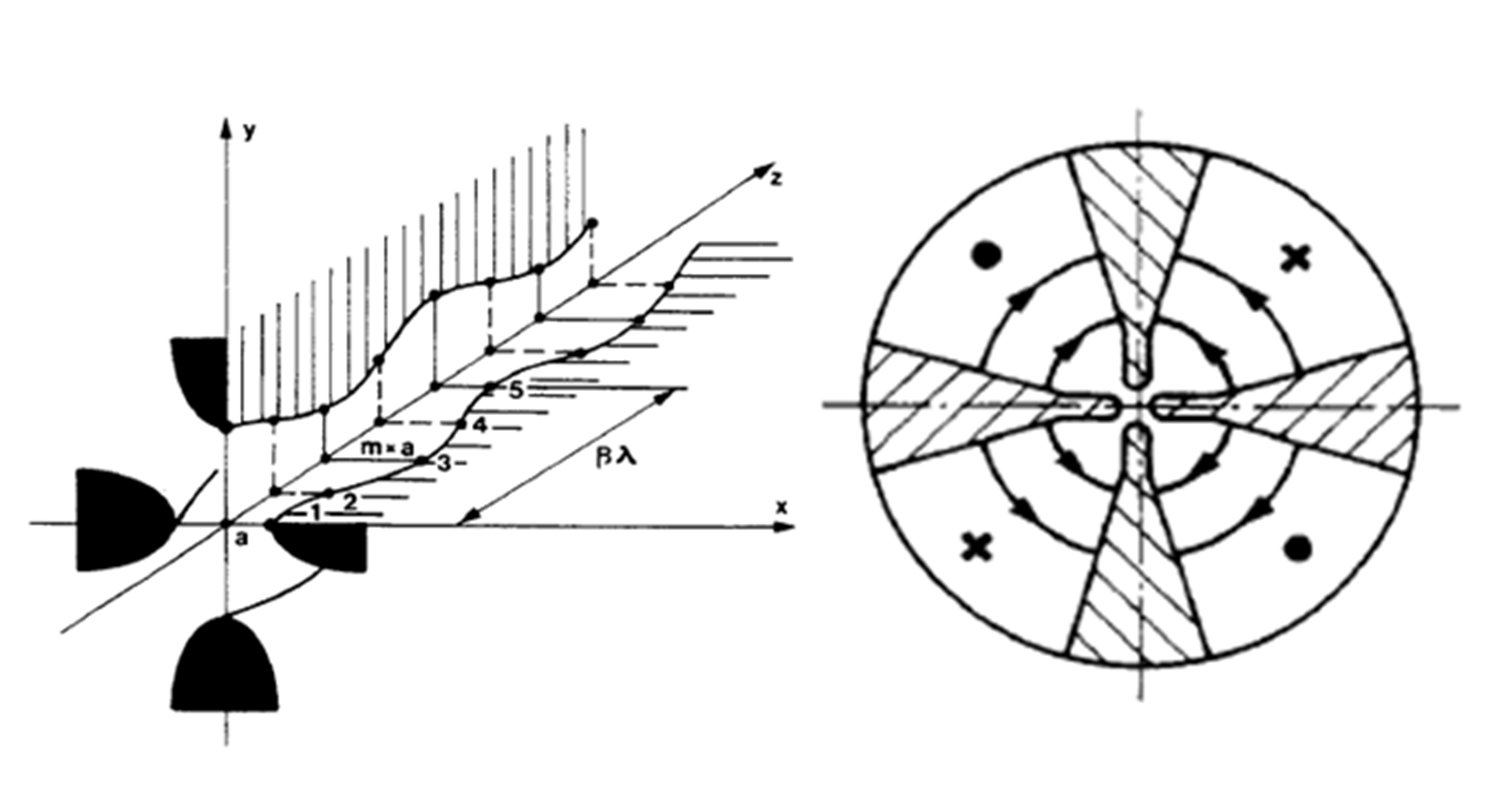
\includegraphics[width=\textwidth]{Figures/LHC_Diagrams/LHC__Linac2__RFQ_schematic.jpg}
        \caption{A schematic of a RFQ, showing the modulation of the
          flanges in the longitudinal direction}\label{fig:rfq_schematic}
      \end{subfigure}
       ~ %add desired spacing between images, e. g. ~, \quad, \qquad, \hfill etc.
      % (or a blank line to force the subfigure onto a new line)
      \begin{subfigure}[h]{0.4\textwidth}
        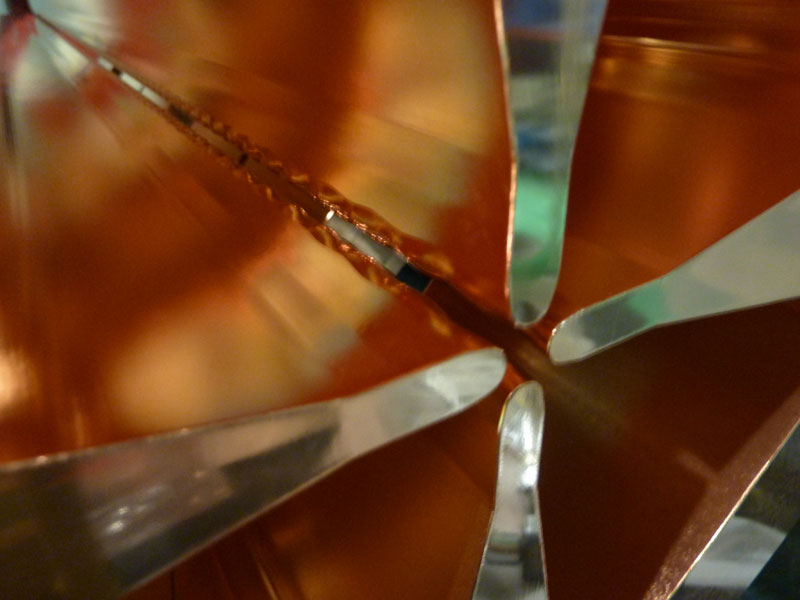
\includegraphics[width=\textwidth]{Figures/LHC_Diagrams/LHC__Linac2__RFQ.jpg}
        \caption{A close-up image of a RFQ, showing the precise
          machining of the longitudanal modulation of the flanges}\label{fig:rfq_actual}
      \end{subfigure}
      ~ %add desired spacing between images, e. g. ~, \quad, \qquad, \hfill etc.
      % (or a blank line to force the subfigure onto a new line)
      \begin{subfigure}[h]{0.4\textwidth}
        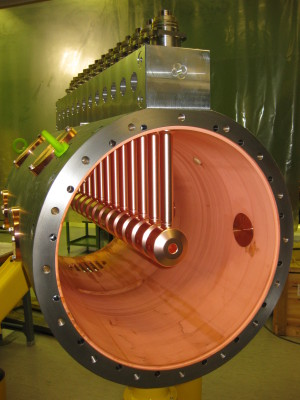
\includegraphics[width=\textwidth]{Figures/LHC_Diagrams/LHC__Linac2__AlvarezTube_Inside__DTL_proto_assembled_image.jpg}
        \caption{The inside of an Alveraz tank, showing the central
          drift tubes, where the protons are accelerated at each gap
          between successive drift tubes}\label{fig:alvarez_tank_inside}
      \end{subfigure}
      ~ %add desired spacing between images, e. g. ~, \quad, \qquad, \hfill etc.
      % (or a blank line to force the subfigure onto a new line)
      \begin{subfigure}[h]{0.4\textwidth}
        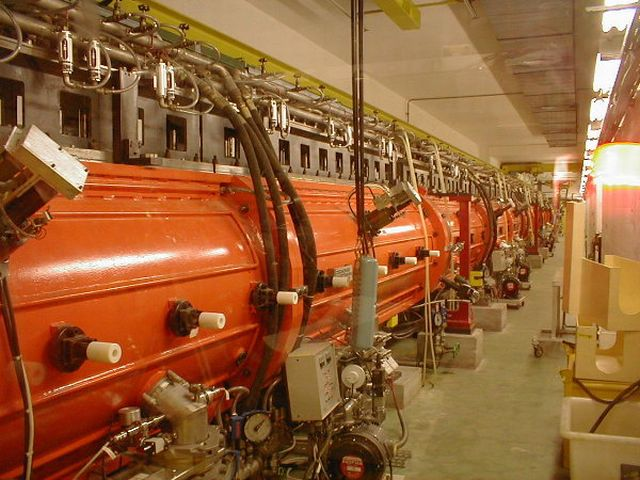
\includegraphics[width=\textwidth]{Figures/LHC_Diagrams/LHC__Linac2__AlvarezTubes.jpg}
        \caption{The Alvarez tanks at the Linac2}\label{fig:alvarez_tank_actual}
      \end{subfigure}
      \caption{Features of the Linac2, the first stage of
        acceleration in the LHC injection chain} \label{fig:linac2}
\end{figure}

\par Protons are initially accelerated by the Linac2 linear accelator
up to 50
\MeV~\cite{LHC:TDR_Vol3_InjectionChain_Benedikt}~\cite{LHC:LHIC_linac2_lhcTests_Hill}.
A bottle of Hydrogren is attached to a duoplasmatron source.  This
device ionizes the Hydrogren, and creates a 300 mA beam of protons,
through a high-voltage anode, and a geometry designed to focus and
collimate the beam as it leaves the device.  Figure
\ref{fig:linac2}(\subref{fig:duoplasmatron_schematic}) shows a
schematic for this device, showing the gas input on the left, and
proton beam leaving to the right.  Figure
\ref{fig:linac2}(\subref{fig:duoplasmatron_actual}) shows the actual
device used in the Linac2 at CERN.  The proton beam then enters the
Radio-Frequency Quadropole (RFQ) system, which accelerates and bunches
the protons up to 750 keV.  The RFQ is a waveguide with four flanges,
which have been machined with a sinusoidal modulation in the
longitudanal direction, which creates an standing electric wave in
this direction, accelerating the protons.  Figure
\ref{fig:linac2}(\subref{fig:rfq_schematic}) shows a schematic of this
modulation, and figure \ref{fig:linac2}(\subref{fig:rfq_actual}) is a
close-up image of this modulation in an actual RFQ. The last stage of
acceleration is provided by three Alvarez tanks.  Each Alvarez tank
holds a series of elctrically isolated cylinders, known as drift
tubes, coaxial with the main tank, with gaps in between them. An
alternating electric field is present in the gaps, and space between
each drift tube and the walls of the tank.  Protons passing through
the center of the drift tubes feel no electric field, but the gaps are
located such that, a proton will always see an accelerating field in
the gap, and are thus receive a boost of energy from each gap as it
traverses the length of the three tanks.  Figure
\ref{fig:linac2}(\subref{fig:alvarez_tank_inside}) shows an image of
the inside of an Alvaez tank, and figure
\ref{fig:linac2}(\subref{fig:alvarez_tank_actual}) shows the tanks at
the Linac2 at CERN.  The final product is a 180 mA, 50 \MeV proton
beam, which is steered to the Proton Synchrotron Booster for the next
stage of acceleration.

\begin{figure}{h}
    \centering
    \begin{subfigure}[h]{0.4\textwidth}
        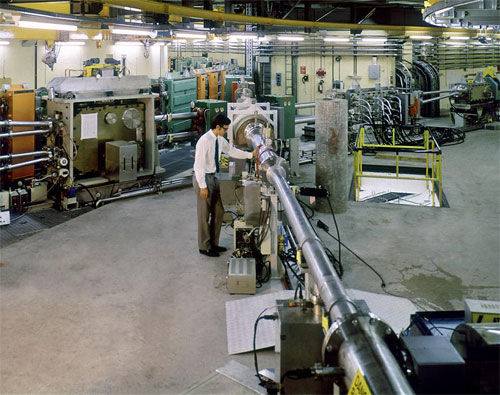
\includegraphics[width=\textwidth]{Figures/LHC_Diagrams/LHC__PSbooster__psb_injection.jpg}
        \caption{The Injection site from the Linac2 into the PS booter}\label{fig:linac2_to_psbooster_injection}
      \end{subfigure}
      ~ %add desired spacing between images, e. g. ~, \quad, \qquad, \hfill etc.
      % (or a blank line to force the subfigure onto a new line)
      \begin{subfigure}[h]{0.4\textwidth}
        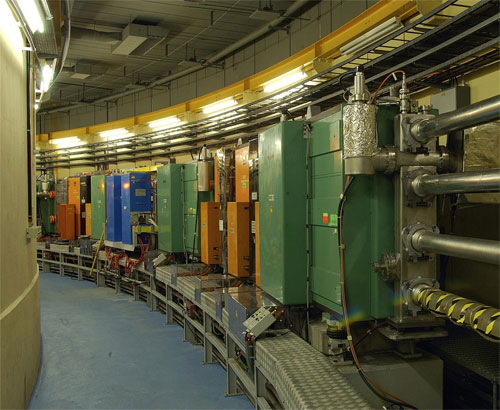
\includegraphics[width=\textwidth]{Figures/LHC_Diagrams/LHC__PSbooster__psb_4_beamLines_shown.jpg}
        \caption{A section of the PS booster, with the four stack
          synchotron beamlines shown in the lower right hand side of the picture}\label{fig:psbooster_4stacks}
      \end{subfigure}
       ~ %add desired spacing between images, e. g. ~, \quad, \qquad, \hfill etc.
      % (or a blank line to force the subfigure onto a new line)
      \begin{subfigure}[h]{0.4\textwidth}
        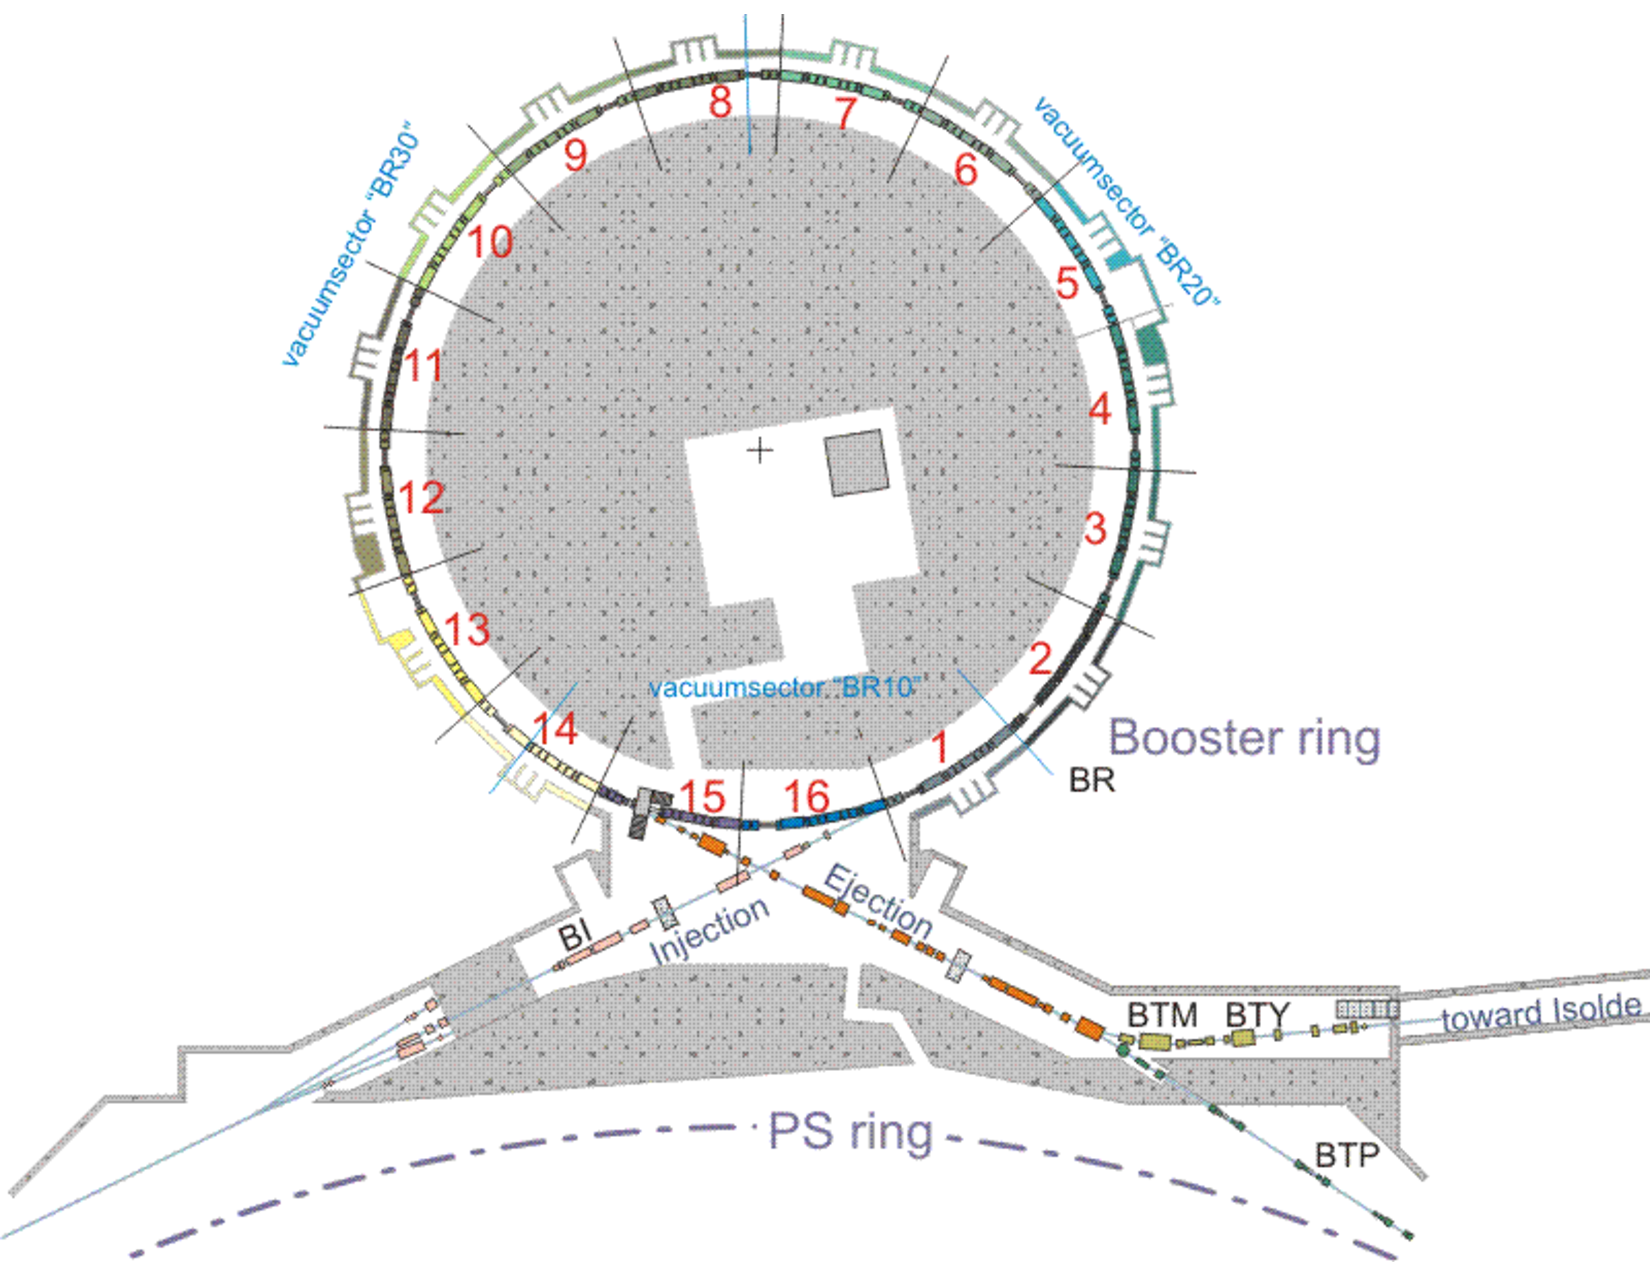
\includegraphics[width=\textwidth]{Figures/LHC_Diagrams/LHC__PSbooster__Layout.pdf}
        \caption{A drawing of the 16 sections of the PS booster}\label{fig:psbooster_16sections}
      \end{subfigure}
       ~ %add desired spacing between images, e. g. ~, \quad, \qquad, \hfill etc.
      % (or a blank line to force the subfigure onto a new line)
      \begin{subfigure}[h]{0.4\textwidth}
        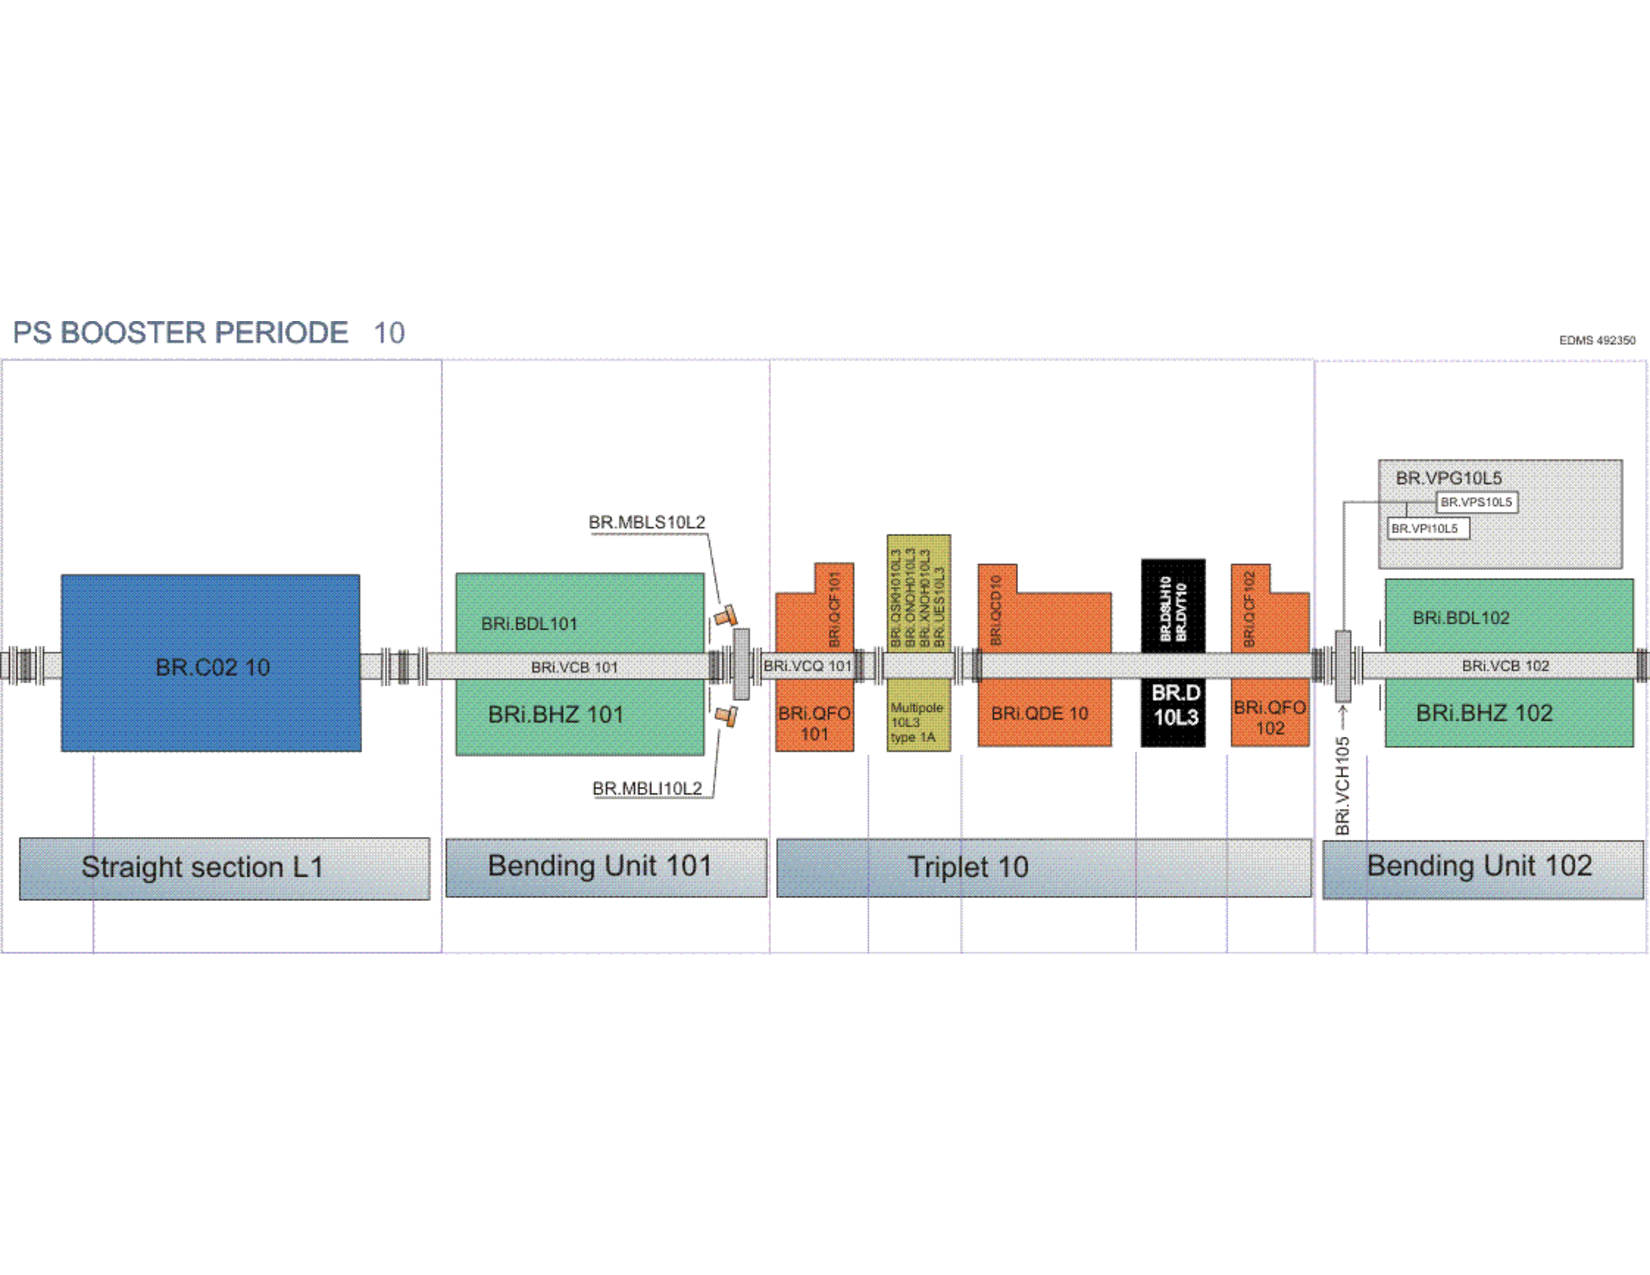
\includegraphics[width=\textwidth]{Figures/LHC_Diagrams/LHC__PSbooster__sect10.pdf}
        \caption{Section 10 of the PS booster.  This begins with the
          CO2 cavity, the main driver of the acceleration; followed by
        a dipole magnet, a triplet of focusing magnets, and a second
        dipole magnet}\label{fig:psbooster_section10}
      \end{subfigure}
      ~ %add desired spacing between images, e. g. ~, \quad, \qquad, \hfill etc.
      % (or a blank line to force the subfigure onto a new line)
      \begin{subfigure}[h]{0.4\textwidth}
        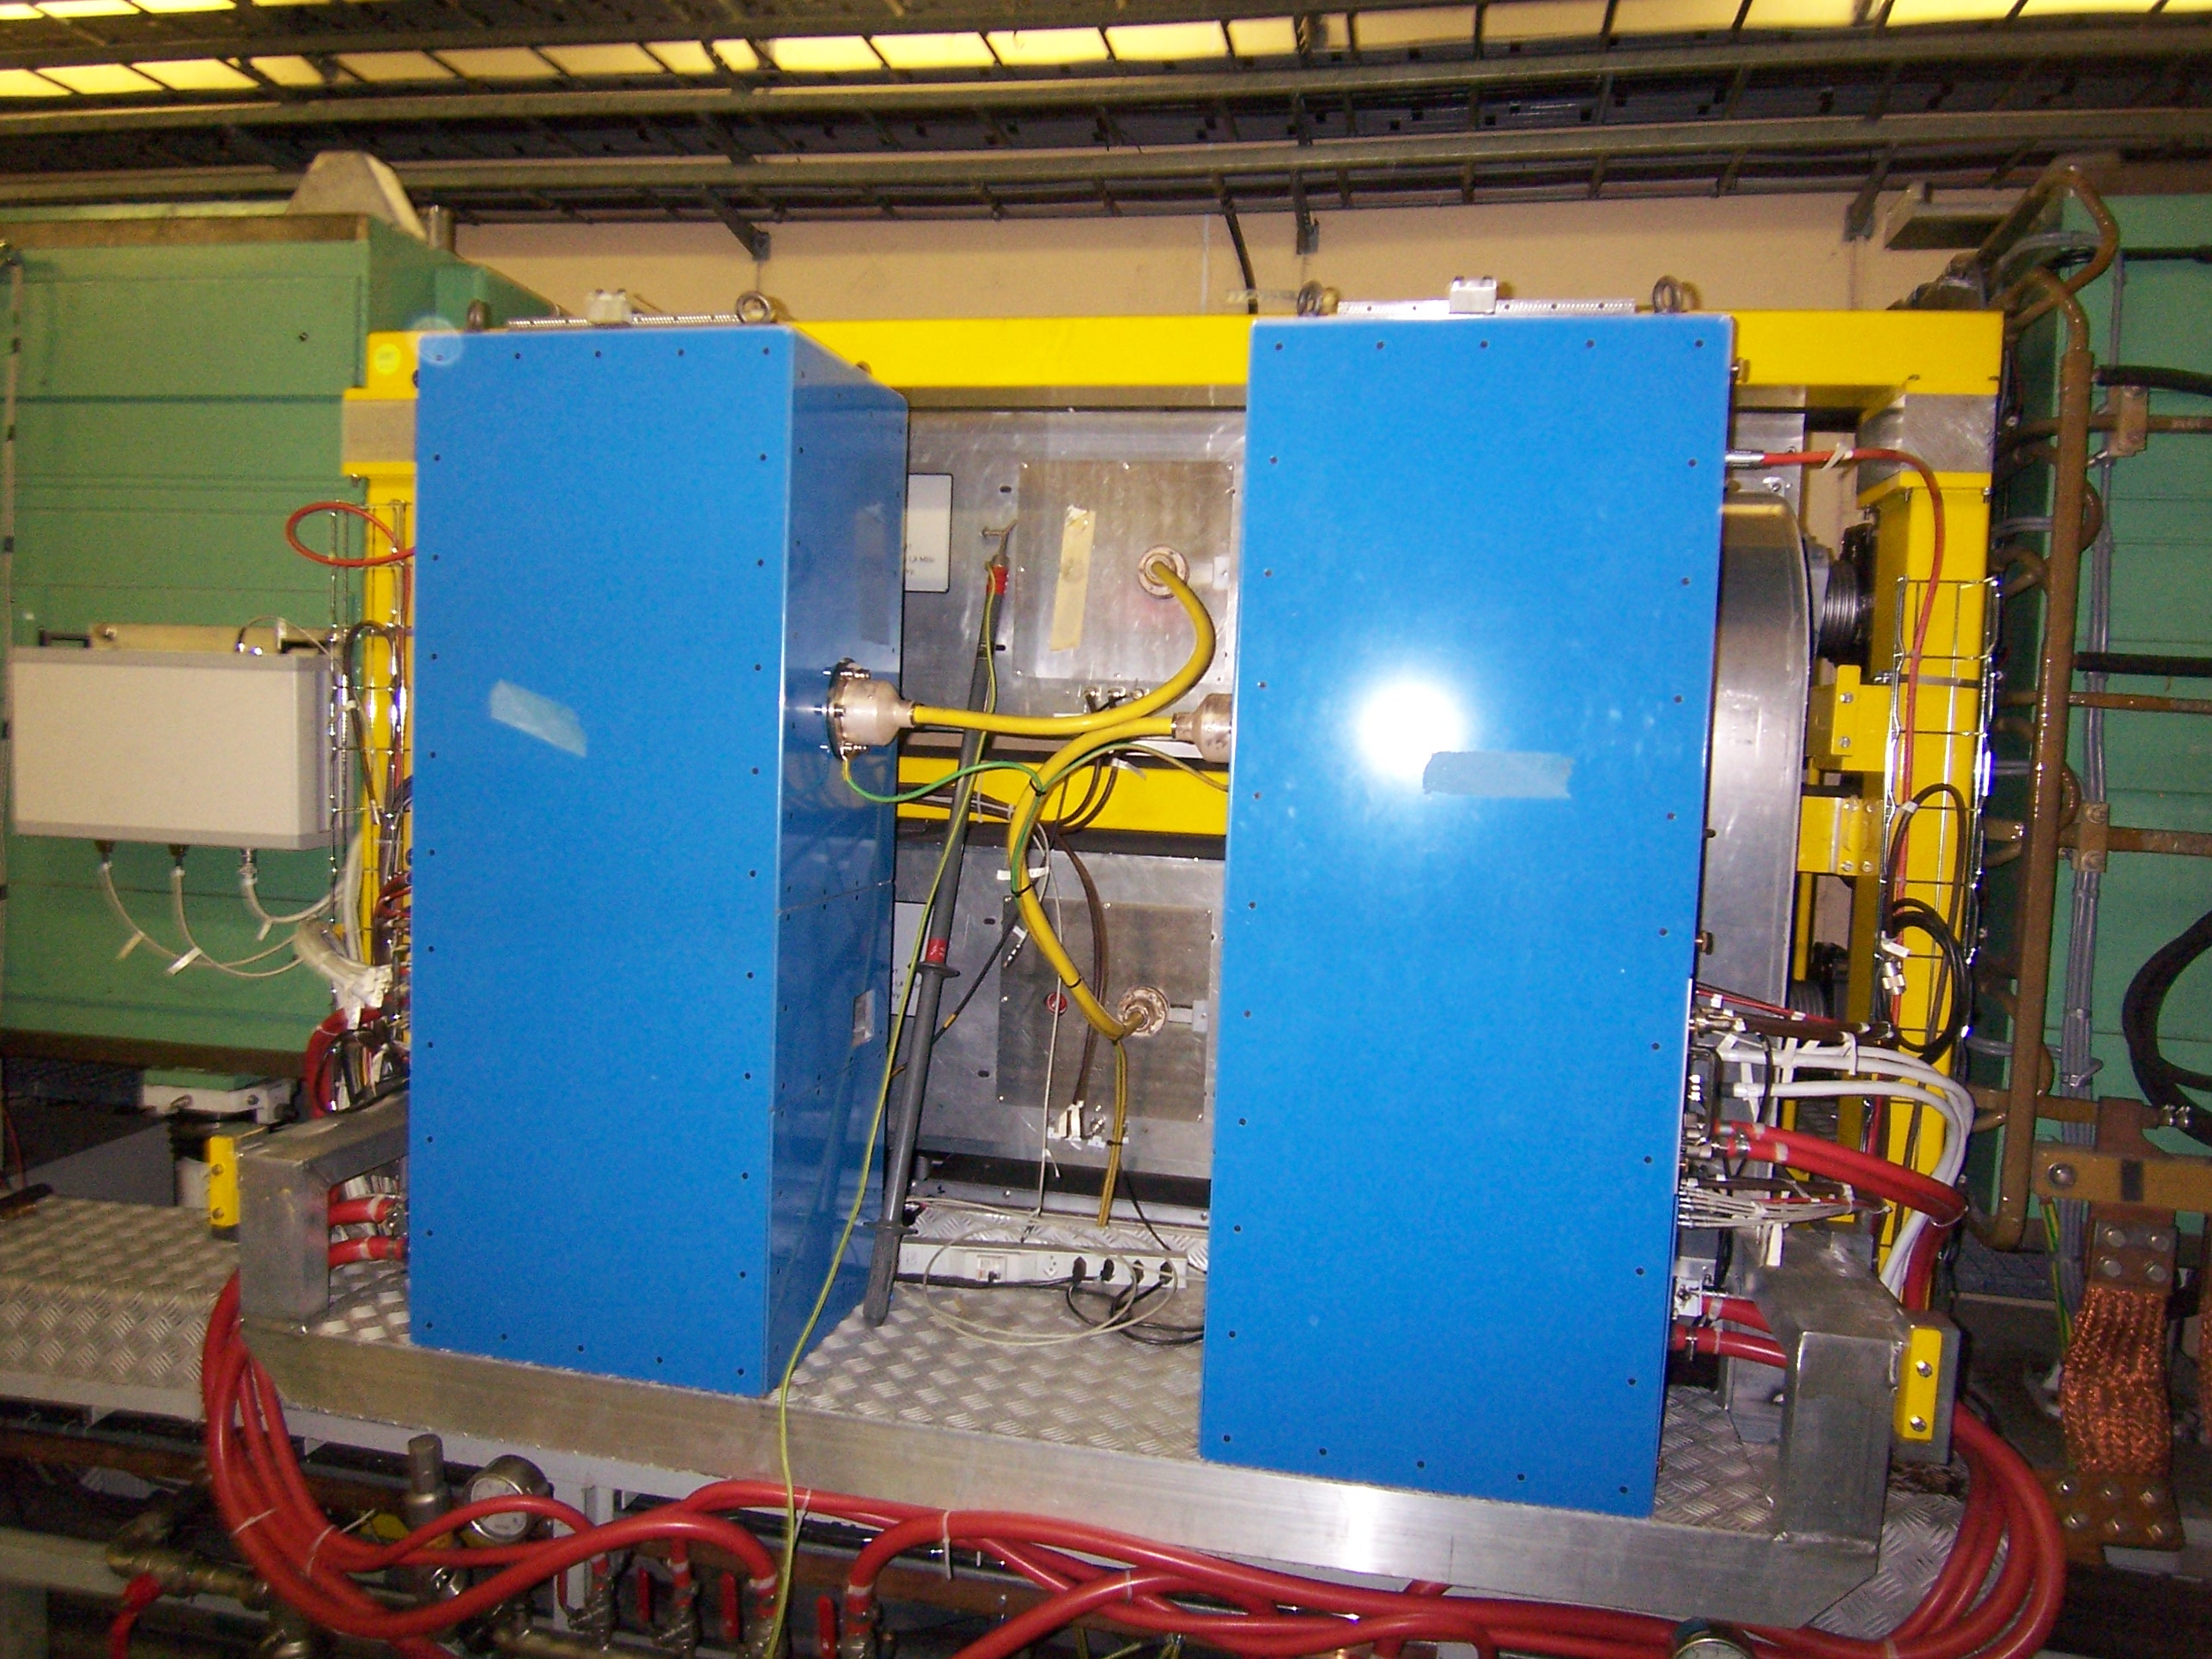
\includegraphics[width=\textwidth]{Figures/LHC_Diagrams/LHC__PSbooster__CO2_RFCavity__P10L1.JPG}
        \caption{A picture of the CO2 RF Cavity, which provides the
          priniciple acceleration for the protons in the PS booster}\label{fig:psbooster_CO2_RFCavity}
      \end{subfigure}
      ~ %add desired spacing between images, e. g. ~, \quad, \qquad, \hfill etc.
      % (or a blank line to force the subfigure onto a new line)
      \begin{subfigure}[h]{0.4\textwidth}
        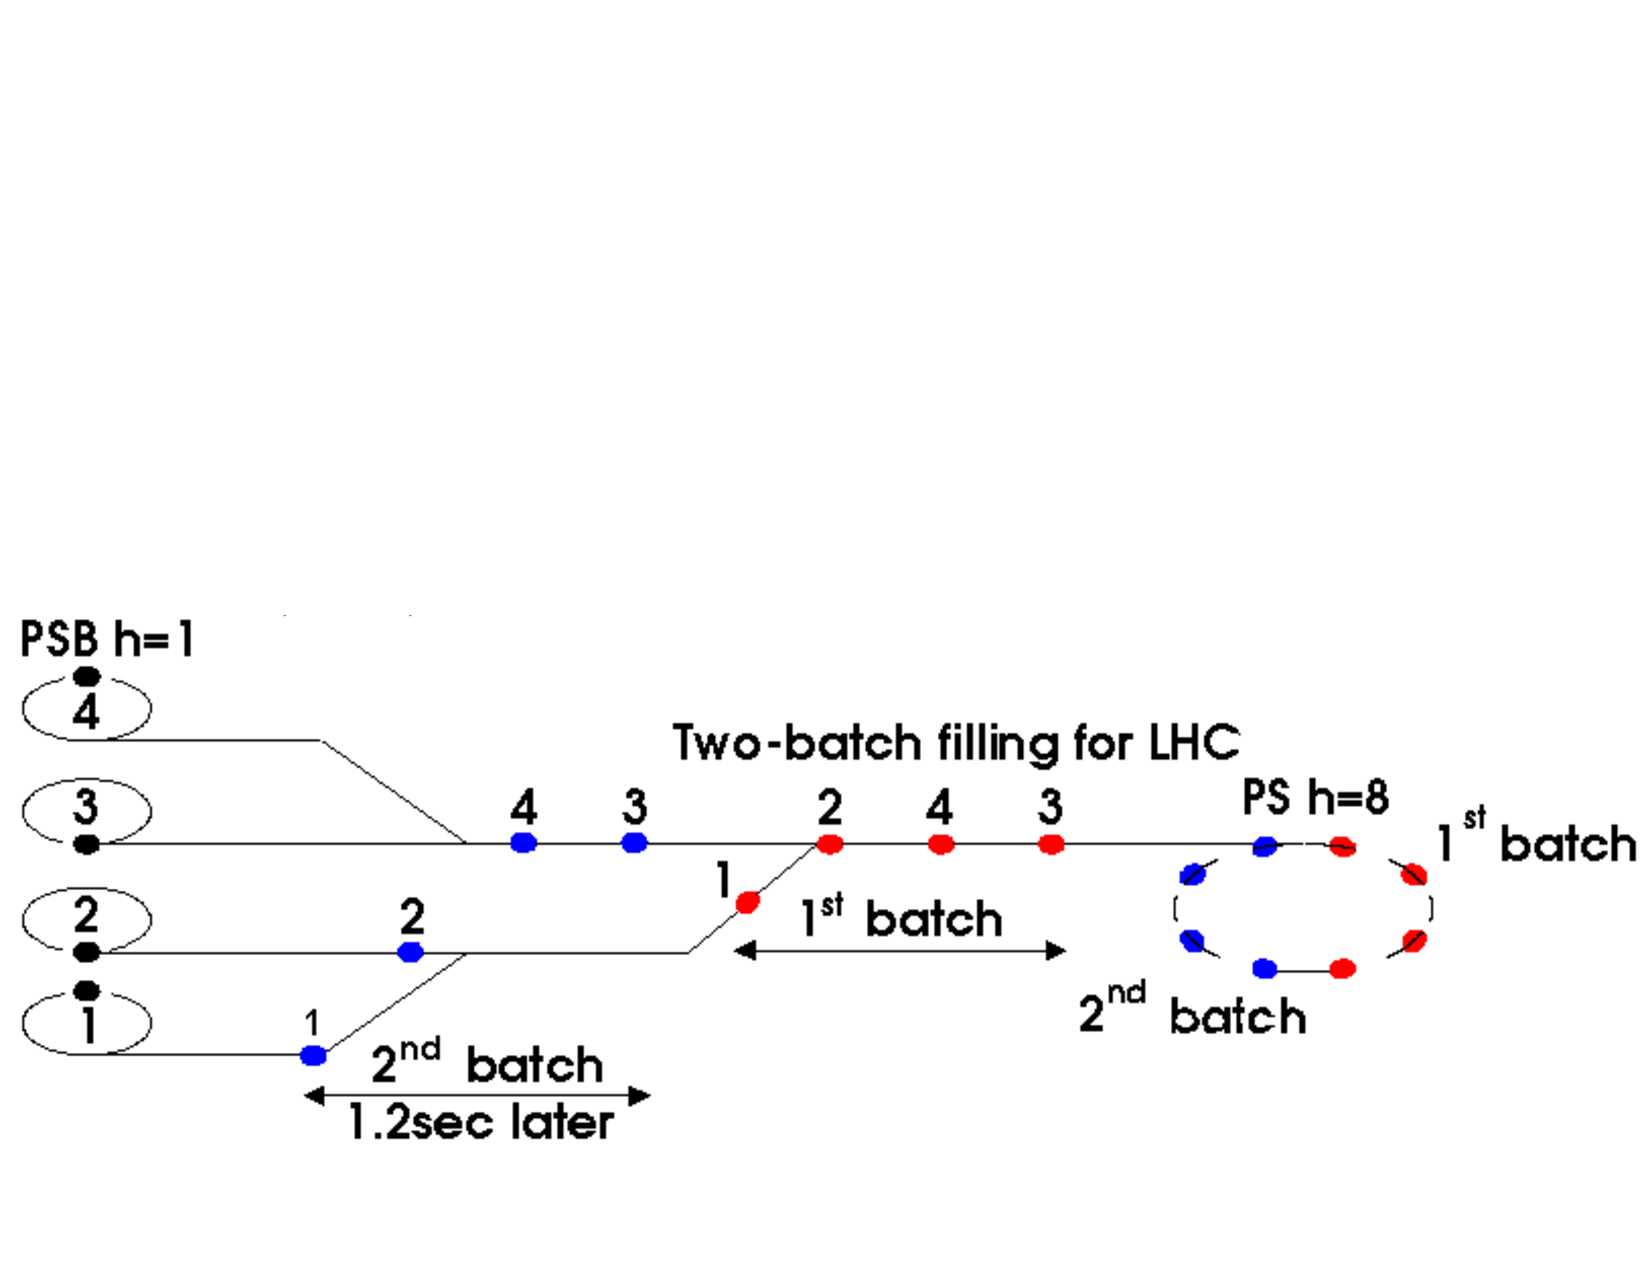
\includegraphics[width=\textwidth]{Figures/LHC_Diagrams/LHC__PSbooster__2batchFillingScheme__schindlrf.pdf}
        \caption{The two batch filling scheme for the PS.  It takes
          1.2 s for each batch to be accelerated from 50 \MeV to 1.4 \GeV}\label{fig:psbooster_2batchScheme}
      \end{subfigure}
      \caption{Features of the PS booster, the second stage of
        the LHC injection chain}\label{fig:psbooster}
\end{figure}

\par The Proton Synchotron Booster (PS booster) complex accelerates
the protons up to 1.4
\GeV~\cite{LHC:TDR_Vol3_InjectionChain_Benedikt}.  The complex takes
the proton beam from the Linac2 and splits the beam into four
separate, synchrotrons, stacked on top of one another.  Figure
\ref{fig:psbooster}(\subref{fig:linac2_to_psbooster_injection}) shows the
injection site of the proton beam from the Linac2 into the PS booter.
The right side of figure
\ref{fig:psbooster}(\subref{fig:psbooster_4stacks}) shows the four
synchotron beam pipes stacked vertically on top one another.  The
splitting of the beam is done in order to reduce the effect of the
space charge of the proton beam, which would increase the transverse
emmitance beyond a tolerable degree.  The PS booster uses thirty-two
0.87 T dipole magnets to bend the beams, and fourty-eight quadrupoles
to focus the beam as it makes its way around each of the 50 m diameter
rings.  Each magnet is composed of a vertical stack of four magnets,
one for each of the synchotrons, and share a common yoke, allowing one
power supply to provide the current to all of them in 
series~\cite{LHC:LHC_psbooster_boosterTurns40}.  The booster is
divided into 16 arcs, as shown in figure
\ref{fig:psbooster}(\subref{fig:psbooster_16sections}).  Each arc contains
a bending dipole, 3 focusing quadrupoles, and a second bending dipole,
followed by a straight section containing beam diagnostic, injection
and ejection systems, and in three sections, the Radio-Frequency (RF) cavities, which is
the mechanism of accelerating the
beam~\cite{LHC:LHC_psbooster_layout}.  Figure
\ref{fig:psbooster}(\subref{fig:psbooster_section10}) shows the layout
of the tenth arc, which also contains one of the RF cavities in the first
section.
  
\par An RF cavity is a specially shaped, hollow
conductor, that the beam passes
through~\cite{LHC:BasicsOfAccelerators_Baird}.  The shape of the
cavity determines the resonant frequency and harmonics (integer
multiples of the fundamental frequency), of the standing
electromagnetic fields that result when the cavity is driven by an
alternating voltage source.  The idea is to choose a resanant
frequency such that the proton will always experience a positive
electric field, and thus an acceleration, each time it passes through
the RF cavity.  This means that the revolution requency of the proton
must be equal to the fundamental frequency or harmonic of the RF
cavity, $f_{RF} = n{\times}f_{rev}$, with $n=1,2,3...$.  Eventually,
the proton is accelerated up to an equilibrium speed and will enter the
cavity just as the standing electric field is alternating through it's
zero point.  If arrives too early for this (moving too fast), then it
will experience a negative electric force, a decceleration, which will
eventually bring it back to the equilibrium revolution frequency,
where it experiences zero net force.  A diffuse beam of protons will
be bunched into groups of protons through this effect as well, as the
faster protons in the beams are deccelerated, and the slower ones
accelerated, until they all reach the same equilibrium revolution
frequency.  Driving  the RF cavity with a harmonic, n, of the proton's
revolution speed will thus create n bunches of protons.  Each one of
the potential n bunch positions is referred to as a bucket.  In the
case where a proton has to be accelerated through a wide range of
energies, the frequency of the cavity must also increase to maintain
synchronization with the proton revolution frequency.  

\par Three types of RF cavities are used to accelerate the beam
during each revolution.  The first of the three types of RF cavities
is the CO2, with frequency range of 0.6 to 2.0 MHz and is used to
drive the $h=1$ harmonic of the  synchrotron, and is pictured in
figure \ref{fig:psbooster}(\subref{fig:psbooster_CO2_RFCavity}).  The
second type of cavity is the CO4 chamber, with a frequency range of
1.2 to 3.9 MHz, and drives the $h=2$ mode of the synchrotron.  This
second mode is capable of spliting the beam and creating two separate
bunch  structures.  However, for LHC running, only one bunch is used,
and is driven primarily by the $h=1$ mode.  The $h=2$ mode is
supplemental and is used to shape the beam.  A third type of RF
cavity, CO16, has a frequency range of 5 to 16 MHz, and is used to
control the longitudal shape of a bunch during acceleration. The beam
leaves the PS booster and enters the PS in a two-batch filling scheme,
taking only 1.2 s to accelerate a second batch of protons from 50 \MeV
to 1.4 \GeV.  This second batch enters just as the first batch has
traveled to the opposite side of the PS ring.  A schematic of this
process is shown in figure
\ref{fig:psbooster}(\subref{fig:psbooster_2batchScheme}).  To acheive
the 25 ns bunch spacing design of the LHC, only 6 bunches of proton
beam need to be delivered to PS.  This is acheived by either using a
4+2 or 3+3 filling scheme, in terms of the number of proton bunches
delived from the four possible synchotrons.   

\begin{figure}{h}
    \centering
    \begin{subfigure}[h]{0.45\textwidth}
        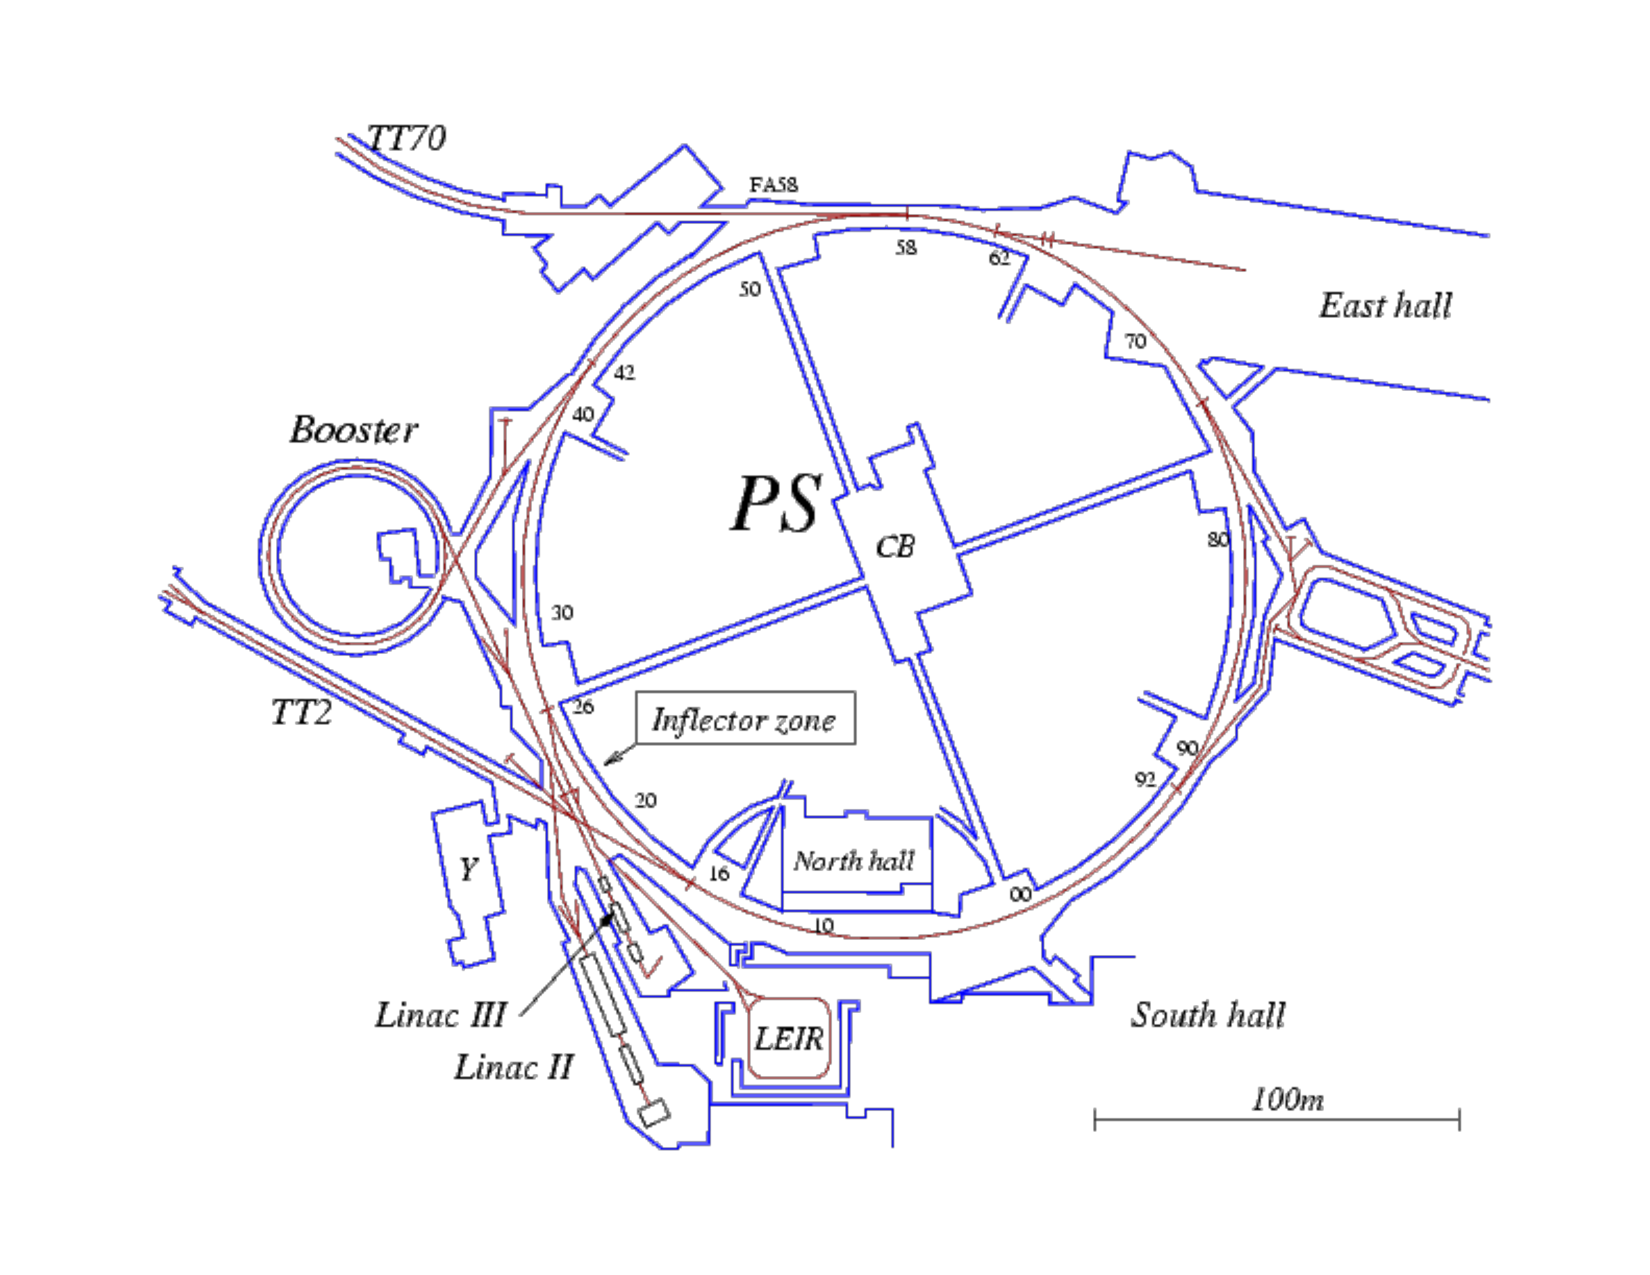
\includegraphics[width=\textwidth]{Figures/LHC_Diagrams/LHC__PS__pscomplex.pdf}
        \caption{A diagram of the PS layout}\label{fig:ps_layout}
      \end{subfigure}
      ~ %add desired spacing between images, e. g. ~, \quad, \qquad, \hfill etc.
      % (or a blank line to force the subfigure onto a new line)
    \begin{subfigure}[h]{0.45\textwidth}
        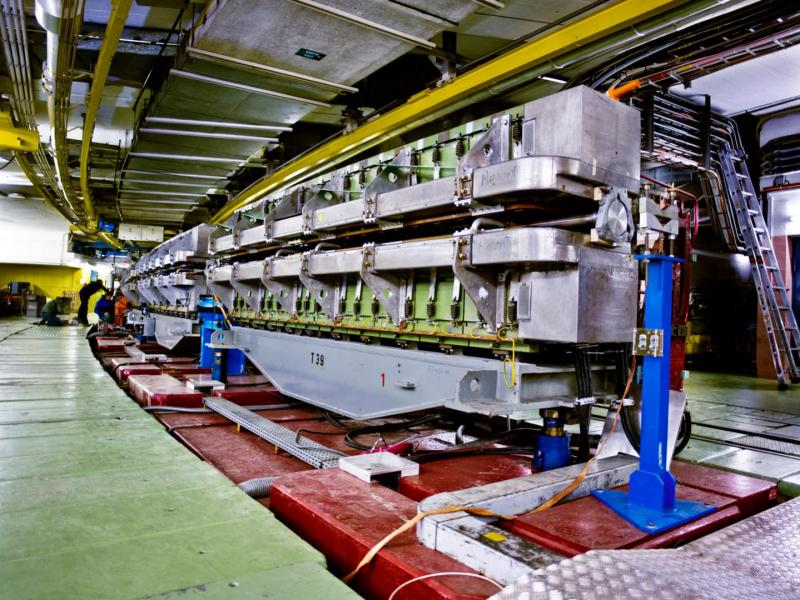
\includegraphics[width=\textwidth]{Figures/LHC_Diagrams/LHC__PS__Dipoles_accelerators-ps.jpg}
        \caption{Dipole magnets used to steer the beam around the 100
          m radius PS ring}\label{fig:ps_dipoles}
      \end{subfigure}
      ~ %add desired spacing between images, e. g. ~, \quad, \qquad, \hfill etc.
      % (or a blank line to force the subfigure onto a new line)
      \begin{subfigure}[h]{0.45\textwidth}
        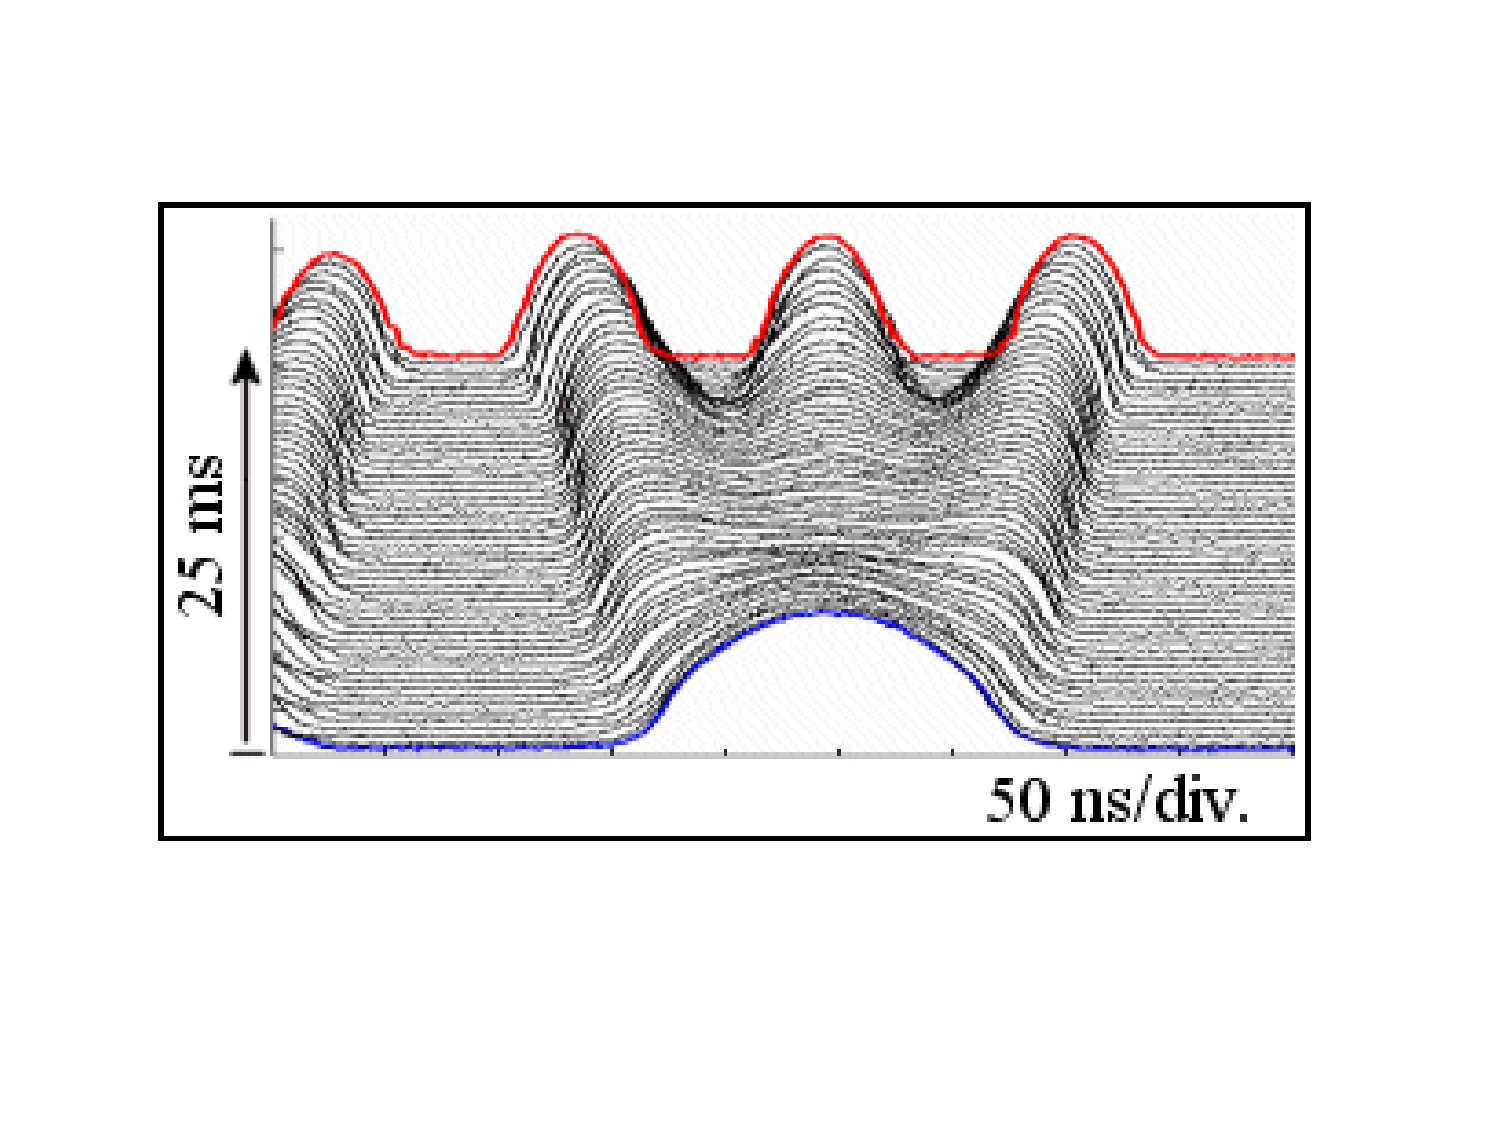
\includegraphics[width=\textwidth]{Figures/LHC_Diagrams/LHC__PS__TripleBunchSplitting.pdf}
        \caption{A simulation of the PS using the $h=7,14,21$ modes of
        to split the beam into 3 bunches}\label{fig:ps_split3}
      \end{subfigure}
       ~ %add desired spacing between images, e. g. ~, \quad, \qquad, \hfill etc.
      % (or a blank line to force the subfigure onto a new line)
      \begin{subfigure}[h]{0.45\textwidth}
        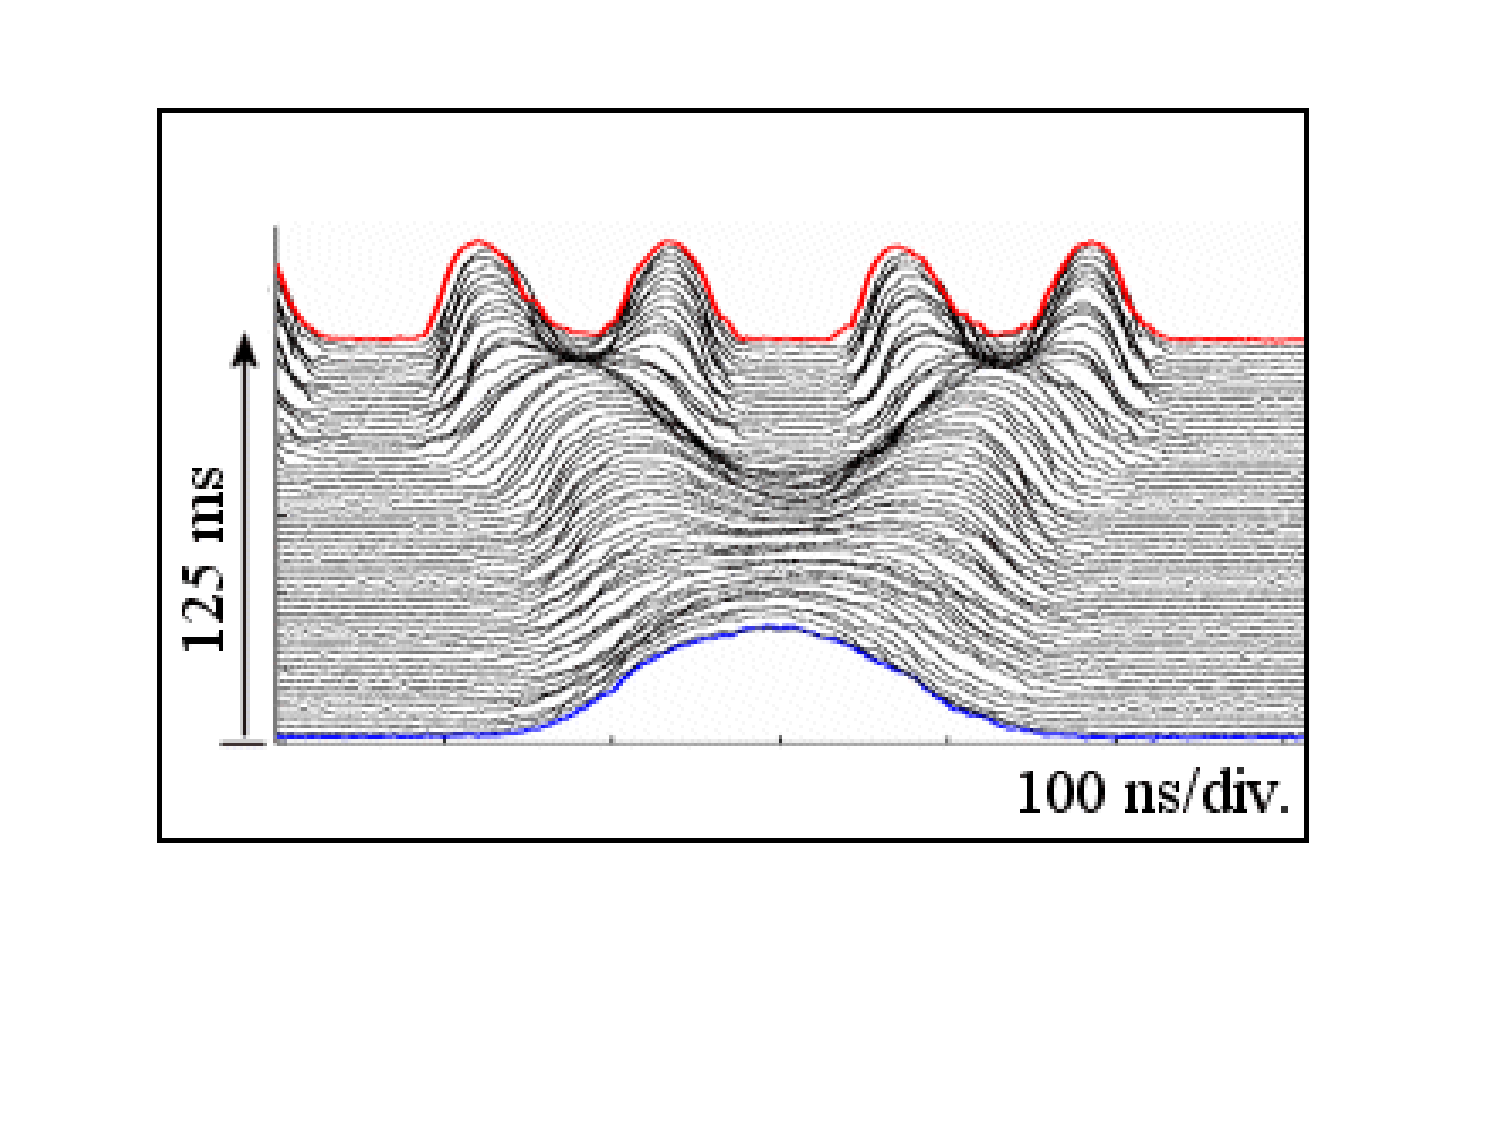
\includegraphics[width=\textwidth]{Figures/LHC_Diagrams/LHC__PS__DoubleDoubleBunchSplitting.pdf}
        \caption{A simulation of the }\label{fig:ps_split2x2}
      \end{subfigure}
       ~ %add desired spacing between images, e. g. ~, \quad, \qquad, \hfill etc.
      % (or a blank line to force the subfigure onto a new line)
      \begin{subfigure}[h]{0.45\textwidth}
        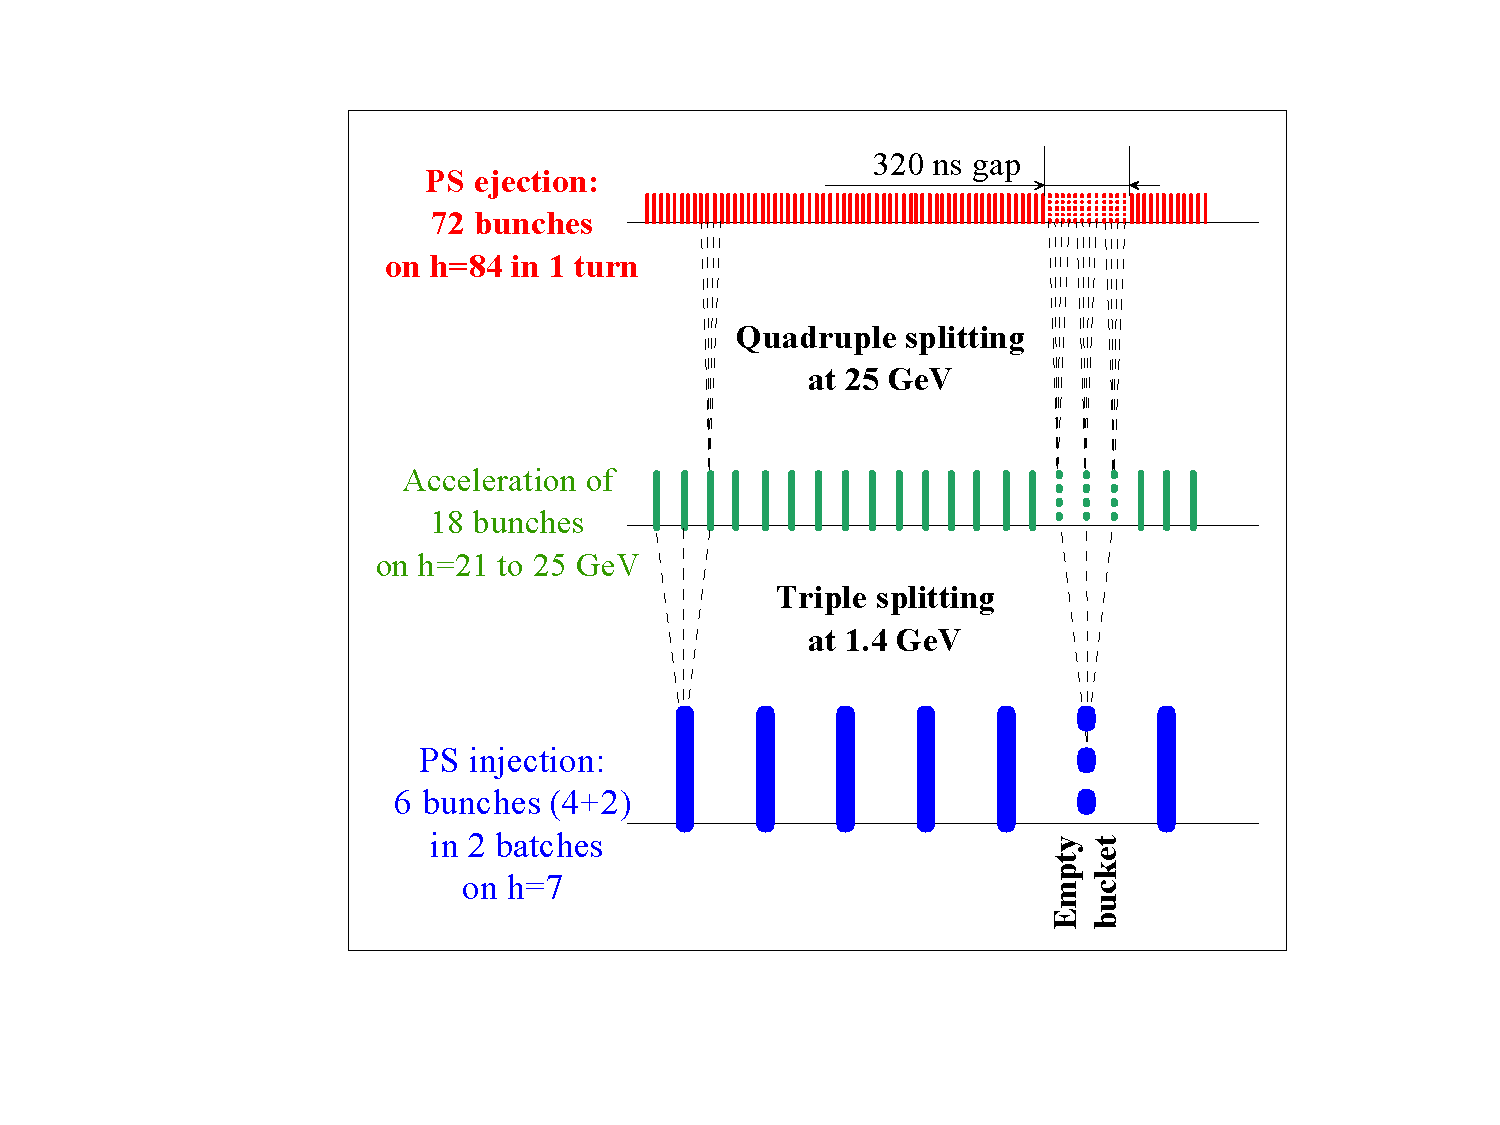
\includegraphics[width=\textwidth]{Figures/LHC_Diagrams/LHC__PS__BunchSplittingDiagram.pdf}
        \caption{An overview of the splitting procedure}\label{fig:ps_splitting}
      \end{subfigure}
      ~ %add desired spacing between images, e. g. ~, \quad, \qquad, \hfill etc.
      % (or a blank line to force the subfigure onto a new line)
      \begin{subfigure}[h]{0.45\textwidth}
        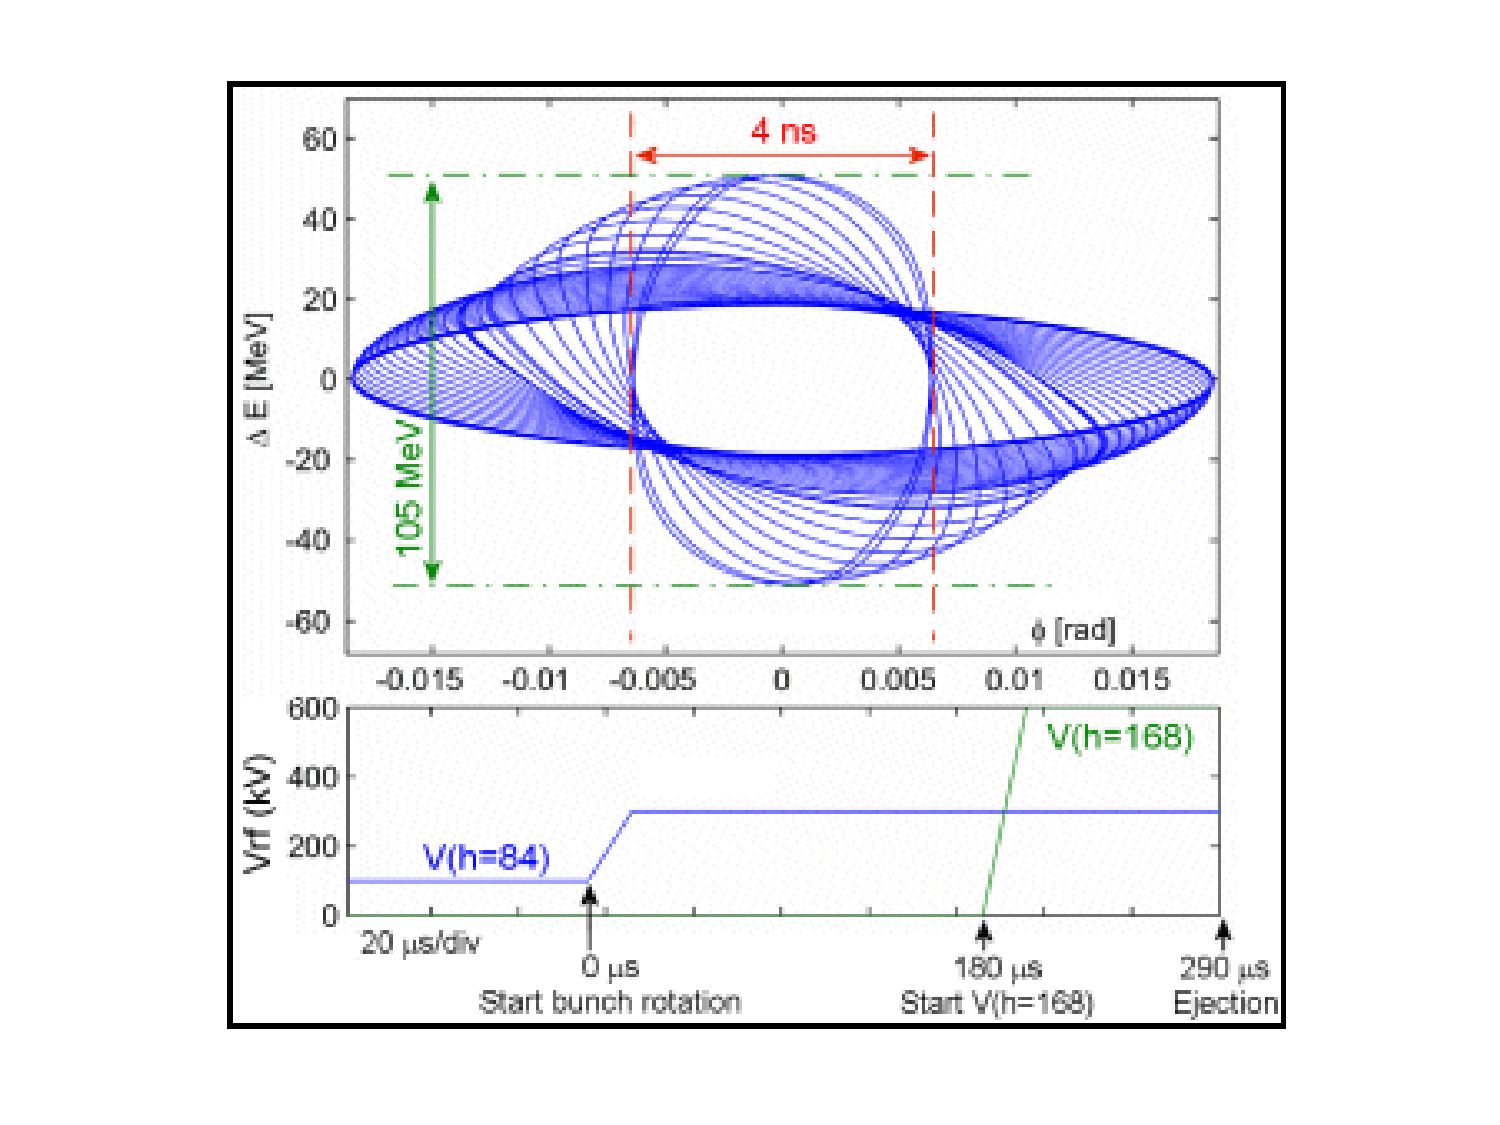
\includegraphics[width=\textwidth]{Figures/LHC_Diagrams/LHC__PS__BunchCompression.pdf}
        \caption{Rotation in phase space of the 25 \GeV proton beam,
          compressing the bunch lengths from 11 ns to 4 ns}\label{fig:ps_bunch_compression}
      \end{subfigure}
      \caption{Features of the PS, the third stage of
        the LHC injection chain}\label{fig:ps}
\end{figure}


\par The next stage is the Proton Synchrotron (PS), which will boost the
protons up to 25 \GeV~\cite{LHC:TDR_Vol3_InjectionChain_Benedikt}.
The layout is shown in figure \ref{fig:ps}(\subref{fig:ps_layout}).  
The ring has a circumfrence of 628 m, and uses 100 dipole magnets and
177 higher-order focusing magnets, to steer the beam around the ring.
Figure \ref{fig:ps}(\subref{fig:ps_dipoles}) shows a picture of one of
the dipole magnets used at the PS.  In addition to providing
acceleration up to 25 \GeV, the PS forms the basis of the bunch
structure that is eventually used in the LHC.  The $h=7$ harmonic is
used to capture the 6 bunches of protons delivered from the PS
booster, leaving a gap in the place of a seventh bunch.  The beam is
then split into three, by using three different RF cavities tuned to
the $h=7,14,21$ modes of the PS.  Figure
\ref{fig:ps}(\subref{fig:ps_split3}) shows a simulation of a proton
bunch being divided  into three over the course of 25 ms.  The $h=21$
mode is then used to accelerate the protons to from 1.4 to 25 \GeV
using the 20 MHz RF cavity.  Each bunch is then split twice,
using the $h=21,42,84$ synchroton modes, to create 72 bunches, spaced
25 ns apart, with a 320 ns gap for the 12 unused buckets of the $h=84$
harmonic. This process is simulated in figure
\ref{fig:ps}(\subref{fig:ps_split2x2}), over the course of 125 ms. The
320 ns gap is created to account for the rise time of the  kicker
magnet, which ejects the beam out of the PS into the SPS.  The entire
splitting process is summarized in figure
\ref{fig:ps}(\subref{fig:ps_splitting}).  For the case of 50 ns bunch
spacing, the final stage of splitting is not performed, and the
$h=21,42$ modes are used to split the beam.  Finally, in order to fit
the bunches into the 200 MHz RF acceleration scheme of the SPS, the 
bunch length must be compressed from 11 ns to 4 ns.  This is acheived
by rotating the beam in the energy vs time phase space by sequential
increases in voltage to the 40 MHz $h=84$ mode, followed by an
increase to the 80 MHz $h=168$ mode.  Figure
\ref{fig:ps}(\subref{fig:ps_bunch_compression}) shows the result of
this rotation - a distortion free ellipse with a smaller 4 ns spread,
but a larger spread in the energy spectrum of the proton beam.   

\begin{figure}{h}
    \centering
    \begin{subfigure}[h]{0.45\textwidth}
        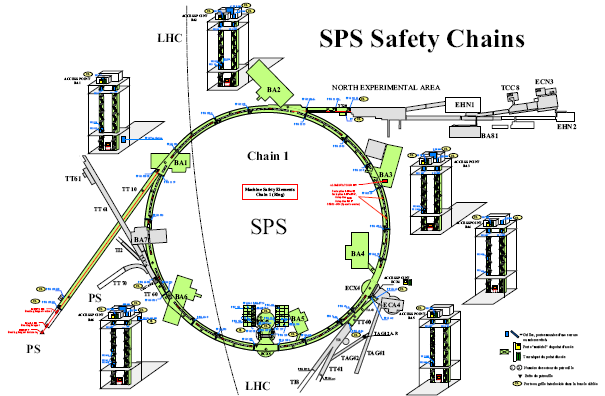
\includegraphics[width=\textwidth]{Figures/LHC_Diagrams/LHC__SPS__layout.png}
        \caption{The layout of the SPS facility}\label{fig:sps_layout}
      \end{subfigure}
      ~ %add desired spacing between images, e. g. ~, \quad, \qquad, \hfill etc.
      % (or a blank line to force the subfigure onto a new line)
    \begin{subfigure}[h]{0.45\textwidth}
        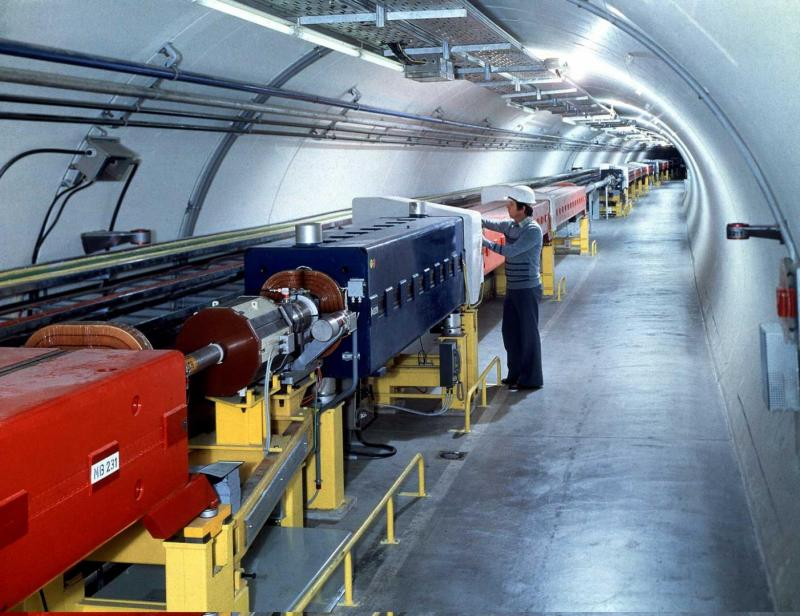
\includegraphics[width=\textwidth]{Figures/LHC_Diagrams/LHC__SPS__beamline.jpg}
        \caption{A sectio of dipole magnets used in the SPS}\label{fig:sps_dipoles}
      \end{subfigure}
      ~ %add desired spacing between images, e. g. ~, \quad, \qquad, \hfill etc.
      % (or a blank line to force the subfigure onto a new line)
      \begin{subfigure}[h]{0.45\textwidth}
        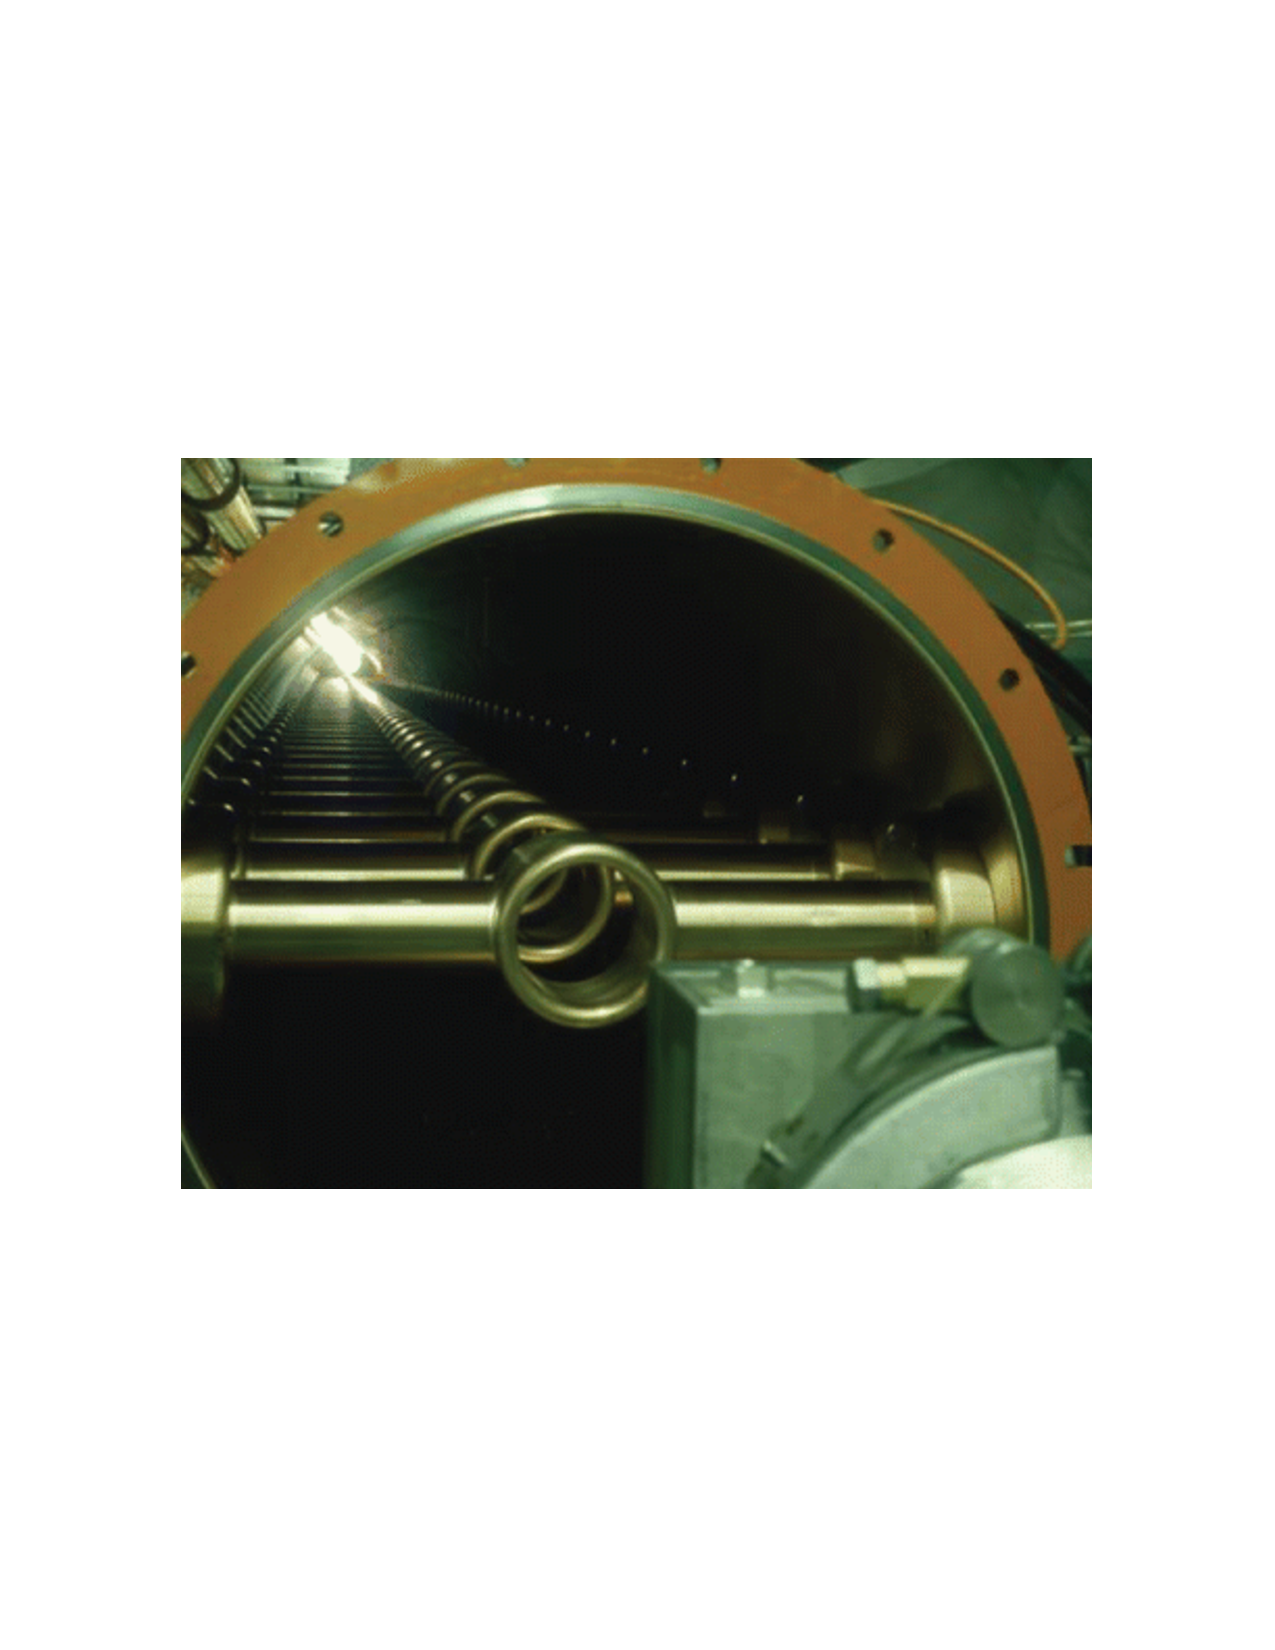
\includegraphics[width=\textwidth]{Figures/LHC_Diagrams/LHC__SPS__RFCavity_InsideView.pdf}
        \caption{The inside of the travelling wave guide structure,
          for the 200 MHz RF cavity in the SPS}\label{fig:sps_rf_inside}
      \end{subfigure}
       ~ %add desired spacing between images, e. g. ~, \quad, \qquad, \hfill etc.
      % (or a blank line to force the subfigure onto a new line)
      \begin{subfigure}[h]{0.45\textwidth}
        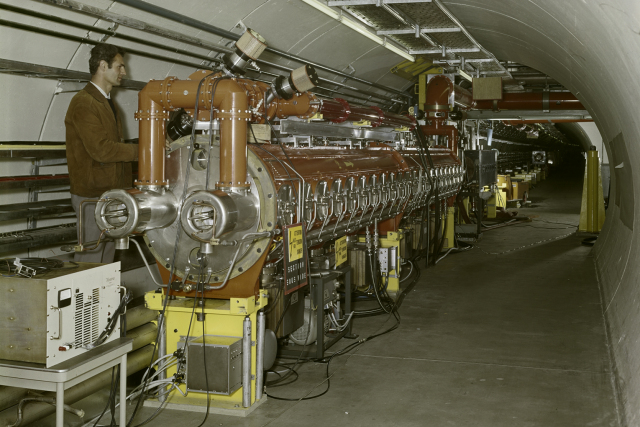
\includegraphics[width=\textwidth]{Figures/LHC_Diagrams/LHC__SPS__RFCavity_OutsideView.jpg}
        \caption{The outside of the 200 MHz RF cavity used to
          accelerate protons from 25 to 450 \GeV }\label{fig:sps_rf_outside}
      \end{subfigure}
       \caption{Features of the SPS, the fourth and final stage of
        the LHC injection chain}\label{fig:sps}
\end{figure}

\par Next, the protons arrive at the Super Proton Synchotron (SPS), where
they will be accelerated to 450 \GeV.  The SPS is the last stage of acceleration
before the protons are injected into the LHC.  The layout is show in
figure \ref{fig:sps}(\subref{fig:sps_layout}).  It has a circumference
of 7 km, and steers the proton beam with 744 dipole magnets, with 573
higher-order focusing magnets~\cite{LHC:LHC_sps_cern_website}.  Figure
\ref{fig:sps}(\subref{fig:sps_dipoles}) shows one of the dipole
mangets in the SPS tunnel.  Like all the other synchrotrons in the
injection chain, the acceleration is provided by RF cavities.  A 200
MHz system of RF cavities capture and fill the SPS by using 2-4
batches of 72 bunch proton beams from the
PS~\cite{LHC:TDR_Vol3_InjectionChain_Benedikt}.  Although the relative
change in frequency is small, the large degree of acceleration
necessitates the use of a tunable RF cavity.  The 200 MHz system has 2
sections of 4 travelling wave cavities in series, and another 2
sections of 5 cavities in series.  Figure
\ref{fig:sps}(\subref{fig:sps_rf_inside}) shows the insde of this
structure, which uses drift tubes to accelerate protons in the gaps
between tubes, with horziontally mounted bars, spaced 374
mm~\cite{LHC:LHC_SPS_200MHzRF_Dôme} apart, determining the periodicity
of the resonant RF field that builds up inside.  The outside of the
structure is shown in figure
\ref{fig:sps}(\subref{fig:sps_rf_outside}).  An additional 800 MHz
system is used to control the transverse emmitance.  It is also used
to stabalize the beam-line and prevent coupled-bunch
instabilities~\cite{LHC:TDR_Vol3_InjectionChain_Benedikt}.  

\par Finally, protons are injected into the LHC ring in one clockwise,
and another counter-clockwise rotating beams.  In order to work in the
limited space of the existing LEP tunnel, the two beams are contained
within a single meachanical and cryostate structure, with a dual-bore
design for each of the beams.  Here, each proton beam is
accelerated to their final energy of 7 \TeV, moving at 99.9999991$\%$
the speed of light, before they meet head on, producing 14 \TeV
center-of-mass collisions.  

\begin{figure}[h]
   \centering
  \includegraphics[width=0.8\textwidth]{Figures/LHC_Diagrams/LHC_Octant.jpg}
  \caption{The LHC ring is divided into eight octants} \label{fig:lhc_octants}
\end{figure}

\par The LHC ring itslef is divided into eight octants, with eight
straight sections that are located in front and behind each of the
eight collision points, where the beams are made to cross and
collide, as shown in figure \ref{fig:lhc_octants}.  These crossings
are known as interaction regions (IRs).  Four of these points are
currently being used by experiments.  TOTEM has detectors on either
side of the CMS experiment at one interaction region, known as point 5
(P5).  LHCf has detectors on either side of ATLAS at point 1 (P1).
MOeDAL has detectors near LHCb at point 8 (P8) and the ALICE detector
is located at point 2 (P2).  The following sections will cover the RF,
magnet, cryogen, and vaccuum technologies used in the LHC ring.  


\section{LHC Magnets}
\label{lhc_magnets}

\par Several types of magnets are used in order to properly circulate
and focus the proton beam as it makes its way around the 26.7 km long
tunnel.  A complete list of all types, can be found in the technical
design report~\cite{LHC:TDR_Vol1_MainRing_Brüning}, as well as through
CERN's outreach web
resources~\cite{LHC:LHC_outreach_listOfAllMagnets}.  This section will
give an overview of the a few of the critical subsystems: the septum
and kicker magnets used for injection from the SPS, the dipole mangets
used for bending the beam around the circumference of the ring, and
the higher-order-pole magnets that are used for focusing the beam.  

\begin{figure}[h]
   \centering
  \includegraphics[width=0.8\textwidth]{Figures/LHC_Diagrams/LHC_SingleTurnInjection.pdf}
  \caption{The single turn injection scheme.  A septum magnet makes
    the initial alignment.  The kicker magnet times the injection and
    makes the final alignment.  Bumper magnets align the LHC beam with
  the injected beam.} \label{fig:lhc_singleTurnInjection}
\end{figure}

\par The injection and extraction of proton beams from one synchrotron
to another involves three types of magnets, septums, kickers, and
bumpers.  Septum magnets contain a partition, or a septum, that
provides a boundary between a high magnetic field region and a
near-zero magnetic field region and are operated in DC or a
slow-pulsed mode~\cite{LHC:LHC_septums_Barnes}.  In case of injecting
a beam of protons into a synchrotron, the target beampipe of the synchrotron
passes through the low-field region, so the trajectory is unaffected
by the high-field region, which bends the injection beam towards the
synchroton alligning it horizontally, with the target beam.  The
kicker magnet, is a fast-pulsed magnet and provides the timing
selection in order to make a final bend vertical bend into the
synchrotron orbit, and into the correct basket of the synchroton bunch 
train~\cite{LHC:LHC_kickers_Barnes}.  Finally, bumper magnets make
small bends to the beam and align it with the injection site.  Figure
\ref{fig:lhc_singleTurnInjection} shows a schematic for this process,
where a transfer line brings protons to a septum, which bends the beam
to a kicker, which makes the final corrections to match the
synchrotron orbit.  For extraction, the kicker magnet quickly
displaces a portion of the beam, which is steered away by the septum,
while the original beam passes through it's low-field region 
unaffected.   

\begin{figure}[h]
   \centering
  \includegraphics[width=0.8\textwidth]{Figures/LHC_Diagrams/LHC_IR8-layout.pdf}
  \caption{Layout of Interaction Region 8, where one proton beam is
    injected into the LHC ring.  A transfer line from the SPS bring a
    proton in from the right.  In green, a septum magnet aligns the
    beam horizontally with the LHC.  In blue, a kicker magnet makes
    the final vertical alignment into the LHC, and is timed to fill
    one of the 400 MHz buckets of the RF capture
    system} \label{fig:lhc_IR8_layout}
\end{figure}

\begin{figure}[h]
   \centering
  \includegraphics[width=0.8\textwidth]{Figures/LHC_Diagrams/LHC_bunchStructure.pdf}
  \caption{The initial filling of 6 batches of protons from the PSB to
  the PS, leaves 12 empty buckets in the PS bunch structure.  The rise
time of the SPS magnet creates an additonal gap in the SPS bunch
structure.  Additional gaps emerge due to the rise time of the LHC
injection and dumping kicker magnets} \label{fig:lhc_bunchStructure}
\end{figure}

\par At the LHC, beam is injected at Interaction Regions (IR) 2 and
8~\cite{lhc:machine_description}.  Two transfer lines bring the beam
extracted from the SPS to $\sim150$ m of the LHC ring.  Five
Labertson-type septum magnets, of field strength $\sim1$ T, are used
to deflect each of the transfer line beams 12 mrad to align the
transfer beam horizontally with the LHC orbit.  Then, four $\sim0.12$T
MKI kicker magnets quickly deflect the beam 0.85 mrad to close the
obrit with the LHC ring.  Figure \ref{fig:lhc_IR8_layout} shows the
layout of the injection point at IR 8.  The green circle encloses the
septum structure, which provides the horizontal alignment, and the
blue encloses the kicker structure, which makes the final vertical
alignment and synchronizes the injection of the beam into the LHC.
The rise time for the field provided by the kicker magets in the LHC
and SPS determine the final bunch structure of the LHC.  Figure
\ref{fig:lhc_bunchStructure} extends figure
\ref{fig:ps}(\subref{fig:ps_splitting}) showing how the rise times of
the kickers that inject, or eject beam create gaps in the bunch
structure of the LHC.  The intial filling of the PS with 6 batches of
protons from the PSB, leaves one initial bucket unused in the PS.
After the splitting of the beam into the 25 ns bunches, there 12 empty
buckets at the of the PS bunch train.  The SPS is filled with three to
four of these trains, leaving an additional 8 25 ns buckets unfilled
due to the 220 ns rise time of the SPS kicker magnet. These three to
four trains are then injected into the LHC, where there are 38 or 39
bunch gaps due to the LHC injector 0.94 $\mu$s rise time.  At the end
of a full LHC orbit, 119 buckets are left empty to allow for the rise
time of the beam dumping kicker magnet, used to remove beam from the
LHC.     

\begin{figure}{h}
    \centering
    \begin{subfigure}[h]{0.450\textwidth}
        \includegraphics[width=\textwidth]{Figures/LHC_Diagrams/LHC_XSec_Dipole_Magnet__LHC-PHO-2001-187.jpg}
        \caption{Cross Section of a LHC dipole magnet}\label{fig:lhc_dipole_xs}
      \end{subfigure}
      ~ %add desired spacing between images, e. g. ~, \quad, \qquad, \hfill etc.
      % (or a blank line to force the subfigure onto a new line)
    \begin{subfigure}[h]{0.450\textwidth}
        \includegraphics[width=\textwidth]{Figures/LHC_Diagrams/LHC_Dipole_CollarAndCoils.jpg}
        \caption{A close-up picture of the non-magnetic collar and
          supercunducting coils of an LHC dipole magnet}\label{fig:lhc_dipole_collarAndCoils}
      \end{subfigure}
      ~ %add desired spacing between images, e. g. ~, \quad, \qquad, \hfill etc.
      % (or a blank line to force the subfigure onto a new line)
      \begin{subfigure}[h]{0.450\textwidth}
        \includegraphics[width=\textwidth]{Figures/LHC_Diagrams/LHC_Dipole_Field.pdf}
        \caption{A simulation of the homogenous, vertical magnetic field lines of the
          dipole. }\label{fig:lhc_dipole_field}
      \end{subfigure}
       ~ %add desired spacing between images, e. g. ~, \quad, \qquad, \hfill etc.
      % (or a blank line to force the subfigure onto a new line)
      \begin{subfigure}[h]{0.450\textwidth}
        \includegraphics[width=\textwidth]{Figures/LHC_Diagrams/LHC_Dipole_ExageratedCurvature.pdf}
        \caption{A diagram showing the exagerated curvature of a
          dipole magnet, with measurements for some of it's most
          important features. }\label{fig:lhc_dipole_curvature}
      \end{subfigure}
      \begin{subfigure}[h]{0.450\textwidth}
        \includegraphics[width=\textwidth]{Figures/LHC_Diagrams/LHC_Dipole_transp-2001-001_05.jpg}
        \caption{A $\sim$15 m long dipole magnet, in a staging area at
        CERN, awaiting installation}\label{fig:lhc_dipole_staging}
      \end{subfigure}
       \caption{Features of the dipole magnets used in the LHC}\label{fig:lhc_dipole}
\end{figure}

\par Once the beam is injected, the curved path around the
circumference of the LHC is maintained via 1232 superconducting dipole
magnets.  The superconducting material niobium-titanium, NbTi, is
cooled to 1.9 K in order to produce the 8.33 T field.  Figure
\ref{fig:lhc_dipole}(\subref{fig:lhc_dipole_xs}) shows a cross-section
view of one of the LHC dipoles.  The dual-bore design of the beam-pipe
is enclosed by an iron yoke, that serves as the cold mass to maintain
the superconducting temperature, and provides a 195 mm gap between
each beam.  A close up picture of the non-magnetic collar and
superconducting coils are shown in figure
\ref{fig:lhc_dipole}(\subref{fig:lhc_dipole_collarAndCoils}).  A
simulation  of the magnet in figure
\ref{fig:lhc_dipole}(\subref{fig:lhc_dipole_field}) shows the
homogenous, vertical magnetic field produced in the center of the
coil.  Diagram \ref{fig:lhc_dipole}(\subref{fig:lhc_dipole_curvature})
shows an exagerated view of the 2812 m radius curvature of each
dipole. However, since each dipole is only $\sim14$ m in length, this
curvature is hardly noticeable, as shown in a photo of an actual
dipole magnet in a staging area at CERN, awaiting installation in
figure \ref{fig:lhc_diple}(\subref{fig:lhc_dipole_staging}).   

\begin{figure}{h}
    \centering
    \begin{subfigure}[h]{0.450\textwidth}
        \includegraphics[width=\textwidth]{Figures/LHC_Diagrams/LHC_Quardupole_Schematic-1998-312.jpg}
        \caption{Cross Section of a LHC quadrupole magnet}\label{fig:lhc_quadrupole_xs}
      \end{subfigure}
      ~ %add desired spacing between images, e. g. ~, \quad, \qquad, \hfill etc.
      % (or a blank line to force the subfigure onto a new line)
    \begin{subfigure}[h]{0.450\textwidth}
        \includegraphics[width=\textwidth]{Figures/LHC_Diagrams/LHC_Quadrupole_TwinMagnets_Staged.jpg}
        \caption{A dual-bore quadrupole magnet, in a staging aread
          prior to installation}\label{fig:lhc_quadrupole_staged}
      \end{subfigure}
      ~ %add desired spacing between images, e. g. ~, \quad, \qquad, \hfill etc.
      % (or a blank line to force the subfigure onto a new line)
      \begin{subfigure}[h]{0.450\textwidth}
        \includegraphics[width=\textwidth]{Figures/LHC_Diagrams/LHC_Quadrupole_Focusing.png}
        \caption{A quadrupole magnet can provide focusing either in
          the horizontal or vertical direction}\label{fig:lhc_quadrupole_field}
      \end{subfigure}
       ~ %add desired spacing between images, e. g. ~, \quad, \qquad, \hfill etc.
      % (or a blank line to force the subfigure onto a new line)
      \begin{subfigure}[h]{0.450\textwidth}
        \includegraphics[width=\textwidth]{Figures/LHC_Diagrams/LHC_MultipoleFields.jpg}
        \caption{Multipole fields from a sextupole and an octupole magnet}\label{fig:lhc_multipole_field}
      \end{subfigure}
      \begin{subfigure}[h]{0.450\textwidth}
        \includegraphics[width=\textwidth]{Figures/LHC_Diagrams/LHC_MagneticCell.png}
        \caption{A typical 110m long magnetic cell at the LHC feturing
        several types of multipole magnets}\label{fig:lhc_magnetic_cell}
      \end{subfigure}
      ~ %add desired spacing between images, e. g. ~, \quad, \qquad, \hfill etc.
      % (or a blank line to force the subfigure onto a new line)
      \begin{subfigure}[h]{0.450\textwidth}
        \includegraphics[width=\textwidth]{Figures/LHC_Diagrams/LHC_InnerTriplet.pdf}
        \caption{Schematic of the Inner triplet structure that brings
          the two serarate beams together in the interagction region}\label{fig:lhc_inner_triplet}
      \end{subfigure}
      ~ %add desired spacing between images, e. g. ~, \quad, \qquad, \hfill etc.
      % (or a blank line to force the subfigure onto a new line)
      \begin{subfigure}[h]{0.450\textwidth}
        \includegraphics[width=\textwidth]{Figures/LHC_Diagrams/LHC_InteractionRegion.jpg}
        \caption{A simulation of two beams being squeezed together by
          the inner triplet.}\label{fig:lhc_beam_squeeze}
      \end{subfigure}
       \caption{Features of the dipole magnets used in the LHC}\label{fig:lhc_multipole}
\end{figure}


\par Quadrupole, septupole, octupole, and other multipole magnets are
used to focus a single beam, as well as squeeze the two beams
together.  There are 392 quadrupole magnets
on the LHC ring, each controlling the height and width of the beam.
Figure \ref{fig:lhc_multipole}(\subref{fig:lhc_quadrupole_xs}) shows a
schematic of a dual-bore quadrupole magnet, and figure
\ref{fig:lhc_multipole}(\subref{fig:lhc_quadrupole_staged}) shows an
actual quadrupole in a staging area before  installation.  Quadrupole
magnets use four sets of coils to create a magnetic field that either
squeezes the beam horizonally or vertically, as shown in figure
\ref{fig:lhc_multipole}(\subref{fig:lhc_quadrupole_field}). Finer
corrections to the beam shape are made with the multipole magnets,
since they are able to compress the beam from more than two axes.
Figure \ref{fig:lhc_multipole}(\subref{fig:lhc_multipole_field})
shows the fields lines of a sextupole and  octuple magnet.  A typical
cell of magnets, 110 m long, in the LHC beamline is shown in a diagram
in figure \ref{fig:lhc_multipole}(\subref{fig:lhc_magnetic_cell}), where the dipole, 
quadrupole and higher order magnet work in series to confine the
protons to the LHC ring.  Finally, a set of single bore magnets, known
as an inner triplet, bring the two beams together into an interaction
region.  Figure
\ref{fig:lhc_multipole}(\subref{fig:lhc_inner_triplet}) shows the
arrangement of magnets that squeeze the beam together, while figure
\ref{fig:lhc_multipole}(\subref{fig:lhc_beam_squeeze}) shows a
simulation of the beams being brought together to collide in the
interaction region.  


\section{LHC RF Technology}
\label{lhc_rf_overview}

\begin{figure}{h}
    \centering
    \begin{subfigure}[h]{0.450\textwidth}
        \includegraphics[width=\textwidth]{Figures/LHC_Diagrams/LHC_RFCavity_Schematic-1994-006.jpg}
        \caption{Cross section of a LHC superconducting Radio
          Frequency cavities, which accelerates the beam by imparting
          275 kW of power through a 400 MHz, 16 MV electric field
          resonanting in the cavity.}\label{fig:lhc_rf_xs}
      \end{subfigure}
      ~ %add desired spacing between images, e. g. ~, \quad, \qquad, \hfill etc.
      % (or a blank line to force the subfigure onto a new line)
    \begin{subfigure}[h]{0.450\textwidth}
        \includegraphics[width=\textwidth]{Figures/LHC_Diagrams/LHC_RFCavity_Staged.jpg}
        \caption{A picture of a four chamber RF cavity in a staging
          area, prior to installation}\label{fig:lhc_rf_staged}
      \end{subfigure}
      ~ %add desired spacing between images, e. g. ~, \quad, \qquad, \hfill etc.
      % (or a blank line to force the subfigure onto a new line)
      \begin{subfigure}[h]{0.450\textwidth}
        \includegraphics[width=\textwidth]{Figures/LHC_Diagrams/LHC_RFCavity_Installed.jpg}
        \caption{The four chamber RF cavity installed at Point 4 of
          the LHC}\label{fig:lhc_rf_at_p4}
      \end{subfigure}
      \caption{Features of the 400 MHz superconducting RF system used in the LHC}\label{fig:lhc_rf}
\end{figure}

\par The LHC uses a 400 MHz superconducting RF cavity system to
capture and accelerate the beam from 450 \GeV to 7
\TeV~\cite{lhc:machine_description}.  Two independent system are used
to provide 8 MV of RF voltage at injection at 16 MV during equilibrium
at 7 \TeV and deliver 275 kW of power to each beam.  This is provided
by 16 niobium sputtered cavities, housed in 4.5 K refrigeration units,
known as cryomodules, at Point 4 of the LHC octant.  The
superconducting material covering the inside of the cavity has
near-zero resistivity, which dissapates much less power and has a much
narrower resonance width, or Q-factor, than a cavity made from
normally conducting material. Figure
\ref{fig:lhc_rf}(\subref{fig:lhc_rf_xs}) shows a schematic of a four
cavity cryomodule.  The beam pipe passes through the center of each
chamber and longtitudinal (left to right in the diagram) electric
fields accelerate the protons each time they circulate the LHC
ring. Figure \ref{fig:lhc_rf}(\subref{fig:lhc_rf_staged}) shows an
actual four cavity module in a staging area prior to installation.  In
this picture, the resonance cavities are concealed underneath the
cyclidrical housing of the vacuum tank and cryostat.  Figure
\ref{fig:lhc_rf}(\subref{fig:lhc_rf_installed}) is a picture of the
module installed at Point 4.  The thin cylindrical structures
extending off the top is the LHe intake valve and quench system.  The
thicker cylindrical structures are the waveguides that couple the
cavities to the source of the electric field, the klystrons.   

\begin{figure}[h]
   \centering
  \includegraphics[width=0.8\textwidth]{Figures/LHC_Diagrams/LHC_KlystronBasic.pdf}
  \caption{A klystron uses a weak RF signal coupled to a resonace
    cavity to bunch an electron beam, which in turn creates an
    amplified RF signal as it passes through a second resonance cavity
    tuned to the same frequency.} \label{fig:lhc_klystron_operation}
\end{figure}

\par A Klystron is the source of RF power that builds up as a
resonance in the cavities that accelerate the protons.  Figure
\ref{fig:lhc_klystron_operation} shows a diagram of the basic
operating principle.  The device uses an anode to accelerate the
thermionic emission of electrons off of a cathode material into one or
more bunching cavities tuned to the frequency the device is designed
to produce.  This cavity is driven with a weak RF source, that groups
electrons into bunches.  Just as discussed for protons earlier, when
electrons arrive at the entrance of the cavity at just the right time,
it will experience the zero-point of the oscillation of the resonating
electric field.  If it arrives early or late, it is accelerated or
decelerated and thus bringing it closer to its neighbors, and
increasing the density of the beam.  After passing through multiple
chambers, the tightly bunched electrons enter a catcher cavity tuned
to the same resonance frequency.  As the electrons pass through at
this resonance frequency, standing electric waves are exicited and
quickly build up in the catcher cavity.  The electron beam is thus
used to amplify the original RF signal in the catcher cavity, which is
then transported via waveguide to power the RF cavity used to
accelerate the proton beamline.  

\begin{figure}[h]
   \centering
  \includegraphics[width=0.6\textwidth]{Figures/LHC_Diagrams/LHC_Klystron_Installed.jpg}
  \caption{One of sixteen 300 kW, 400 MHz klystrons that power the
    superconducting RF cavities that accelerate the proton beam.} \label{fig:lhc_klystron}
\end{figure}

\par At the LHC, 16 400 MHz, 300 kW kylstrons, work together to provide 4800 kW
of power to the superconducting RF
cavities~\cite{lhc:machine_description}.  They are also located at
Point 4, in the UX45 service cavern adjacent to the RF cavities, about
6 m below the beamline.  An average of 22 m of waveguide is used to
transport the power generated by the klystrons to the RF cavities.
Figure \ref{fig:lhc_klystron} shows a klystron installed at the LHC, and like most modern
klystrons, it also utilizes a multi-bunching chamber design.

\section{The LHC Cryogen System}
\label{lhc_cryogen_overview}

\begin{figure}[h]
   \centering
  \includegraphics[width=0.6\textwidth]{Figures/LHC_Diagrams/LHC_CoolingPlants.pdf}
  \caption{Layout of the five cryogenic islands, which are home to the
  eight facilities that provide liquid helium to the LHC} \label{fig:lhc_cryogenic_islands}
\end{figure}

\par The LHC is the largest cryogenic system in the
world~\cite{LHC:LHC_lhc_cryogen_cernWebsite}, as its operating
temperature is 1.8 K, in order to produce the high-magnetic fields
needed by the dipole magnets.  Addtionally, the acceleration,
mechanism, the RF cavities, are also superconducting, and must be
cooled to 4.5 K.  Over 120 tons of Helium are used as the cryogenic
medium, since once it is cooled below 2.17 K, it becomes a superfluid,
a phase of matter with a high thermal conductivity, making it ideal
for refridgeration.  Cryogenic and auxillary equipment are
concentrated into 5 \"cryogenic islands\" at Points 1,2,4,6, and
8~\cite{lhc:machine_description}.  As shown in figure
\ref{fig:lhc_cryogenic_islands}, Point 4,6, and 8 house two facilities
each, making a total of eight, one for each octant of the LHC arc. 

\begin{figure}{h}
    \centering
    \begin{subfigure}[h]{0.450\textwidth}
        \includegraphics[width=\textwidth]{Figures/LHC_Diagrams/LHC_Cryogen_4p5KFridgeCompressor.pdf}
        \caption{The compressor station for the 4.5 K refridgeration system}\label{fig:lhc_cryo_4p5_compressor}
      \end{subfigure}
      ~ %add desired spacing between images, e. g. ~, \quad, \qquad, \hfill etc.
      % (or a blank line to force the subfigure onto a new line)
    \begin{subfigure}[h]{0.450\textwidth}
        \includegraphics[width=\textwidth]{Figures/LHC_Diagrams/LHC_Cryogen4p5KFridge_Coldbox.pdf}
        \caption{The 4.5 K refridgeration system cold box, containing
          heat exchanging fins and turbins to cool the He}\label{fig:lhc_cryo_4p5_coldbox}
      \end{subfigure}
      \caption{Features of the 4.5 K refridgeration system}\label{fig:lhc_cryo_4p5}
\end{figure}

\par At each cryogenic plant, He is cooled to 80 K by cirulating it
through refridgeration equiptment with liquid nitrogen in the heat
exchangers\cite{LHC:LHC_lhc_cryogen_cernWebsite}.  Next, the He is
brough to 4.5 K with refridgerators recovered from the LEP experiment
\cite{LHC:LHC_cool_challenge}.  The He gas is first compressed and allowed
to expand, where it is cooled by losing energy through mechanical
turbo-expanders that run at up to 140,000 rpm on helium-gas
bearings.  Figure
\ref{fig:lhc_cryo_4p5}(\subref{fig:lhc_cryo_4p5_compressor}).  The He
is then liquified after passing through a vacuum sealed box containing
heat exchangers and more turbo-expanders
\cite{LHC:LHC_cryogenicHe_system_Lebrun}. The compressor for this
system is pictured in figure
\ref{fig:lhc_cryo_4p5}(\subref{fig:lhc_cryo_4p5_coldbox}).  Finally,
the liquified He is brought to 1.8 K with a refrigeration unit that
uses a cold compression train to decrease the saturation pressure, and
thus temperature as well. 

\begin{figure}[h]
   \centering
  \includegraphics[width=0.6\textwidth]{Figures/LHC_Diagrams/LHC_CryogenInTunnel.pdf}
  \caption{Cross section schematic of the cryogenic distribution
    system in the LHC tunnel} \label{fig:lhc_cryogen_tunnel_xs}
\end{figure}

\par In the LHC tunnel, a cryogenic distribution line runs parallel to
the machine \cite{LHC:LHC_cool_challenge}.  It consists of eight 3.2
km long cryostats, that contain the equipment to supply and recover
helium with temperatures ranging from 4 K to 75 K.  A total of 310
service modules, are used to control the system and provide safety
mechanisms against pressure buildup and magnet quenching.  Figure
\ref{fig:lhc_cryogen_tunnel_xs} shows a cross section of the cryogen
distribution system in the tunnel. 

\section{The LHC Vacuum System}
\label{lhc_vacuum_overview}

\par The LHC is also the largest operational vacuum system in the
world and is capable of achieving pressures lower than outer space
\cite{LHC:LHC_lhc_vacuum_cernWebsite}.  Three different types of
vacuum systems are used: one for insulating the helium distribution
lines, another for insulating the dipole magnets, and a final
ultra-high vacuum system for the beam pipe
\cite{lhc:machine_description}.  

\par The vacuum systems for insulating the helium distribution and
dipoles involves some 104 km of piping an over 250,000 welding
joints \cite{LHC:LHC_lhc_vacuum_cernWebsite}.  Pressure here is
required to be kept at $10^{-1}$ mbar, but at cryogenic temperatures,
pressuers tend to equalize at a much lower level, to $10^{-6}$ mbar
($\sim10^{-9}$ atm) \cite{lhc:machine_description}.   

\begin{figure}[h]
   \centering
  \includegraphics[width=0.6\textwidth]{Figures/LHC_Diagrams/LHC_BeamScreen.jpg}
  \caption{Beam screen for the LHC, with slits to allow for easy
    pumping of residual gas molecules in the beampipe.} \label{fig:lhc_beam_screen}
\end{figure}

\par The most stringent requirements come on the vacuum of the
beam-pipe.  The beam must minimize the number of interactions it has
with any particles outside of the interaction region.  A pressure of
$10^{-10}$ to $10^{-11}$ mbar are maintained in the 54 km of
beampipe \cite{LHC:LHC_lhc_vacuum_cernWebsite}.  Weeks of cryogenic
pumping, eventually condenses gas trapped in the beampipe into a
liquid that can be absorbed by the walls of the beampipe.  The inside
beampipe is also coated with a thin layer of a special substance 
developed at CERN, a titanium-zirconium-vanadium alloy, which absorbs
residual particles when heated.  780 ion pumps are used to remove the
noble gases and methane, which do not interact with the substance,
which acts as its own distributed pumping system.  Room-temperature
sections of the beampipe are also heated to 300$^{\deg}$ to be
baked-out from the outside.  This is done to periodically remove 
any material which may have settled and become trapped. Additionally,
the beam-pipe is designed with a racetrack shape, which optimises the
available aperture while leaving space for the cooling tubes, as shown
in figure \ref{fig:lhc_beam_screen}.  Slits also allow for gas
molecules to be easily pumped out from inside its volume.   


\chapter{The Compact Muon Solenoid}
\label{cms_description_overview}

The \acrfull{cms} is one of two general purpose detectors at the \acrshort{lhc}.  

\section{The Inner Tracker}
\label{inner_tracker_description}

\par The inner tracker is silicon and really really big, lots of
channels.

\section{The Electromagnetic Caliorimeter}
\label{ecal_description}

\par PBWO4 crystals.  APDs in the Barrel.  VPTs in the Endcaps

\subsection{Vacuum Photo-Triodes}
\label{vpt_description}

\par Extra time for VPTs

\subsection{Test Rig at UVa}
\label{vpt_test_rig_description}

\par Big maget, lots of light, test dem led's

\subsection{Results of UVa Tests}
\label{vpt_results_description}

\par Plots, Plots, plots, plots, plots

\section{The Hadronic Caliorimeter}
\label{hcal_description}

\par Brass, Steel, Soviet Sweat

\section{Forward Caliorimetry}
\label{fcal_description}

\par High eta, great for VBF

\section{Magnet and Return Yoke}
\label{magnet_description}

\par Describe solenoid and measuring field, and engineering marvel or
return yoke structure.

\section{Muon Chambers}
\label{muon_chamber_description}

\par APDs DTs and CSCs

\section{Data Collection Overview}
\label{data_collection_description}

\par L1 trigger, HLT etc


\chapter{Particle Reconstruction at CMS}
\label{reconstruction_overview}

\par Data is reconstructed at CMS using the $Particle Flow^{TM}$ algorithm

\section{Muon Reconstruction}
\label{muon_reco_overview}

\par Muons rely heavily on the inner tracker and muons chambers for
efficient identrification and reconstruction

\section{Electron Reconstruction}
\label{electron_reco_overview}

\par Electrons leave charged tracks in the inner tracker, and create a
wide shower of particles and thus energy deposits in the ECAL.  High
energy electrons sometimes traverse the entire distance of the ECAL
and leave energy in the HCAL, however the ratio of these two energies
is disproportionate for the ECAL, and thus this ratio is often used to
discriminate electrons from highly electromagnetic hadronic jets.

\section{Photon Reconstruction}
\label{photon_reco_overview}

\par Like electrons, but with no tracks, and narrower shower shape.

\section{Jet Reconstruction}
\label{jet_reco_overview}

\par Jets are formed by matching tracks from the inner tracker to
energy deposits in the ECAL and HCAL.  Energy clusters are identified
from the ECAL and HCAL, and everything is then clustered in a cone.

\section{Tau Reconstruction}
\label{tau_reco_overview}

\par So heavy that they decay to leptons or hadrons before traversing
the detector, they still leave an oddly-numbered pronged decay hadronically due
to charge conservation requiring that one of the hadrons produced be
eqaul charge to the tau.  This results in one charged, and any number
of neutral pions, or three charged, and any number of neutral pions. 

\section{Missing Transverse Energy Reconstruction}

\par since the detector is hermetic, and the tracker so granular, we
can ensure that no particles flew out of the detector due to lack of
coverage.  Only long-lived neutral particles can escape, such as
neutrinos in the standard model.  Many \acrshort{bsm} theories, such
as SUSY, are characterized by stable, neutral particles. 

\par MET is the vector sum of all of the tracks associated with a
particular primary vertex (? or all vertices in event).  Thus if there
wasa neutral particle that escaped detection, there would be a
momentum imbalance along the trajectory of that particle.  This is how
neutrinos are identified.  

\chapter{Analysis I: The first 5.08 \fbinv of 8 \TeV data}
\label{analysis_1_overview}

\par The search for $t\bar{t}H$ production begins by identifying $pp$
collisions consistent with the production of a top quark pair with
additional $b$ jets.  Top quarks decay $\sim100\%$ of the time to a
bottom quark and a $W$ boson, and the $W$ boson can decay either into
a charged lepton and a neutrino or into a pair of quarks.  Since there are two $W$ bosons in
the event, the decays of the $W$ bosons determine the specific top
pair signatures recorded in the detector.  The decay of the two $W$
bosons define the categorizations of $t\bar{t}$-like events as either
all-hadronic, in the case of zero charged leptons; semi-leptonic, in
the case of one charged lepton; and di-leptonic in the case of two
charged leptons.  the detector. This analysis describes the
Lepton+Jets (LJ) channel, where one of the $W$ bosons has decayed to an
electron or a muon and the corresponding neutrino, while the other $W$
boson decays into two quarks.  To compensate for the low production
rate, the analysis is optimized to search for the Higgs boson decaying
to a $b$-quark pair.  The final state is then $l \nu qqbbbb$, where
$l$ refers to either an electron or a muon.  In the case of an ideal
reconstruction of the event, the LJ signal events contains six jets,
four of which are $b$-tagged. However, to accommodate jets lost to
detector acceptance and merging between separate partons, and the
$b$-tagging efficiency, events with four or more jets and two or more
$b$-tags are included in the signal region.  

\begin{figure}[h]
  \centering
  \includegraphics[width=0.7\textwidth]{Figures/Analysis_1_Diagrams/h_closestDR_mass_tag_tag_ge4t_rebin.pdf}
  \caption{This figure shows the breakdown of jet-to-parton
   assignments for the two jets with the minimum $\Delta R$
  separation in the event for events with greater or equal 4
  $b$-tagged jets.}\label{fig:tagMassCombinatorics}  
\end{figure}

\par The largest background contribution is $t\bar{t}+$jets
production.  This process can be decomposed in terms of the flavour of
the extra jets produced in the event.  For this analysis, the
inclusive $t\bar{t}$jets process is broken into three sub-proccesses:
$t\bar{t}+$ light flavor jets where one or more 
of the jets is mistagged, $t\bar{t}+c\bar{c}$ and $t\bar{t}+b\bar{b}$.
Smaller background contributions come from $W+$jets, $Z+$jets, single
top quark, diboson, and $t\bar{t}+W/Z$ production.  

\par In other Higgs searches involving the decay to two $b$-quarks,
the most powerful discriminating variable is the invariant mass of the
$b\bar{b}$ pair, which has a peak at the mass of the Higgs.  However, for
$t\bar{t}H$ production, with a final state of four $b$-quarks, the
combinatorics of selecting the quarks coming from the Higgs, instead
of the $t\bar{t}$ system, prevents the reconstruction of a clear
resonant peak, as shown in figure \ref{fig:tagMassCombinatorics}.
This results in an additional loss of mass resolution, or smearing,
on the $b\bar{b}$ invariant mass spectrum. 

\par Although there is poor resolution on the Higgs boson resonance in
the $b$-quark dijet mass spectrum, there are a number of kinematic
variables that can be used to discrminate betweenthe $t\bar{t}+$jets
background and the $t\bar{t}H$ signal.  For example, the recoil of
the Higgs off of the $t\bar{t}$ system, the decay products of the top
quarks from the $t\bar{t}H$ signal will have, on average, a slightly
larger component of momentum transverse to the beam-line.
Additionally, the lager number of authentic $b$-jets in $t\bar{t}H$
events can be exploited through the likelihood value returned by a
$b$-tagging algorithm for all of the jets in the event.  By
themselves, none of these variables provide a large degree of
discriminating power to separate the $t\bar{t}H$ signal from the
large, and kinematically similar background.  Therefore, the
discriminating power of several variables is combined using a
multivariate analysis technique (MVA), which is used to set upper
limits on $t\bar{t}H$ production in the data set. 

\par The following sections will describe the analysis that was
carried out on the first 5 \fbinv~of data collected by the CMS
detector.  This includes definitions of the simulatied samples used to
estimate the expected backgrounds in data, the event selection used to
isolate the $t\bar{t}H$ signal, the application of MVA techniques,
evaluation of systematic uncertainties, and upper limit setting on the
production rate of $t\bar{t}H$. 


\section{Data and Simulated Samples}
\label{data_and_mc_overview}

\par $pp$ collision data is collected by the CMS detector, as
described in previous chapters.  The signal and background signatures
are estimated using Monte Carlo simulation techniques.  The simulation
involves the combination of the most current theoretical and emperical
information about the interactions of the known particles.  The
simulation of an event is decomposed into a sequence of calculations and
each signal and background process is calculated seperately.
Information about Monte Carlo event simulation techniques is taken
from reference \cite{Agashe:2014kda}.  

\par The first stage of event simulation for a given signal or
background process is to calculate the probability that some set
initial state particles with a certain momentum will create a final
state of particles with a certain momentum.  For example, in the case of
the \ttH signal, this is the probability that two protons travelling
towards each other along the z-axis (beam-line), each with a given
energy and momentum, will produce a top quark pair and a Higgs boson,
each with some momentum vector, $\hat{p}_{t}$, $\hat{p}_{\bar{t}}$,
$\hat{p}_{H}$, which points into the hermetic CMS detector.  As
discused in section \ref{qft_overview}, this probability is calculated
by examing the lagrangian of the theory describing the process and
calculating its scattering amplitude, to some order in perturbation
theory, using the Feynman rules derived from the lagrangian.  The
scattering amplitude is a multi-dimensional probability function,
which depends on the inital and final state momentum of the particles
in the process.  Thus, given some intial state momentum, $p_{i}$, it tells you
the probability to produce a final state particle with mometum
$p_{f}$.  It is understandable that the scattering amplitude is
often reffered to as a matrix element, since given a vector of initial
state particles with a certain momentum, the scattering amplitude
would be a matrix, whose elements would give the probability of
creating the vector of final state particles.  

\par Since protons are composite objects, when they
collide, it is their quarks or gluons which are actually interacting.
The momentum distribution of each of the valence quarks, the gluons,
and the sea quarks, which account for quantum fluctuations that
temporarily create all other quark flavours inside the proton, is described by
a Parton Distribution Function (PDF).  The PDF describes what fraction
of the proton's momentum is distributed among each of its
constituents.  Due to the large strength of the QCD interactions that
bind the quarks together, the PDF cannot be calculated perturbitavely
from QCD.  It has been measured empircally, and is composition of the
results of several experiments over the past decades.  

\par Event generator algorithms are computer programs
that, given a lagrangian of particle theory, will calculate the
matrix element for a given process.  Then, the generator is provided
with values of the momentum of the intial state particles.  For
protons, this would the beam energy of the LHC.  To assign mometum
values to the constinuent quarks or gluons that actually participate
in the interaction, random values are sampled from the probability
distributions described by a PDF that is provided to the algorithm.
Given a choice of momentum for the input particles, a value and
direction of the momentum for each of the final state particles is
sampled from the probability function provided by the calculated the
matrix element (ME).  The process of randomly sampling a probability
function, in order to conduct a calculation, is known as a Monte Carlo
sampling technique.    

\par In the case where final state particles are quarks or gluons,
also known as partons, an additional calculation is necessary to
create the physical hadron states.  First, the decay sequence of each
parton is calculated until the decay products reach a user defined
value, known as the hadronization scale.  This decay sequence is
referred to as the parton shower (PS), since each parton creates a
multitude, or a shower, of additional partons.  Once the parton shower
is calculated, each of the colored partons are transformed into
color-singlet primary hadrons, which themselves decay, and form
secondary hadrons.  This process, known as hadronization, results in a
collimated spray of hadrons, each with a component of momentum along
the original parton's direction.  These hadrons are clustered together
and referred to as a hadron jet.   

\par Once the hadronization is completed, the next stage of the event
generation is to simulate the response of the CMS detector when this
process occurs at the interaction point where the LHC beams are made
to collide.  The Geant 4 detector simulation framework is used to
create a model of each and every detector element, electronic readout,
and mechanical support structures that make compose CMS.  Geant 4 is
also about to describe how energy is deposited into the different
types of material as a particle passes through each detector element,
simulating the response each element to presence of a particle in the
detector.  The digitization and signal acquisition of the electronics
that read-out the detector elements is also simulated.  

\par The final stage the generation of an event is the reconstruction
of the simulated detector signals into physics objects.  This process
is described in detail in the previous chapter.  It proceeds with
simulated, instead of real detector signals.  

\par The entire event simulation, reconstruction, and subsequent
anlaysis is implemented in a software framework that is known as CMS
Software (CMSSW).  

\subsection{Data Samples}
\label{data_overview}

\par The results presented here are based on the first 5.08\fbinv of the
2012 CMS dataset.  Data-sets are collected through HLT triggers and
stored offline for analysis.  Table~\ref{tab:dataSamples} lists the datasets used
for this analysis, which is composed of two runs of data collection
triggered on the presence of one muon or electron in an event.
The luminosities are quoted from a calculation performed with
minimum-bias events measured with the HF detector and have been
determined to have a 2.2\% uncertainty.   

\begin{table}[hbtp]\footnotesize
\centering
\begin{tabular}{|l|c|r|}
\hline\hline
 Dataset & Run Range & Integrated Luminosity \\
\hline
/SingleMu/Run2012A-PromptReco-v1/AOD & 190645--193621 & 0.87 fb$^{-1}$ \\
/SingleMu/Run2012B-PromptReco-v1/AOD & 193834--196531 & 4.21 fb$^{-1}$ \\
{\bf Total SingleMu} & {\bf 190645--196531} & {\bf 5.08 fb$\mathbf{^{-1}}$} \\
\hline
/SingleElectron/Run2012A-PromptReco-v1/AOD & 190645--193621 & 0.87 pb$^{-1}$ \\
/SingleElectron/Run2012B-PromptReco-v1/AOD & 193834--196531 & 4.21 pb$^{-1}$ \\
{\bf Total SingleElectron} & {\bf 190645--196531} & {\bf 5.08 fb$\mathbf{^{-1}}$} \\
\hline\hline
\end{tabular}
\caption{The datasets analyzed for this analysis.}
\label{tab:dataSamples}
\end{table}

\subsection{Signal Samples}
\label{signal_sample_overview}

\par The $t\bar{t}H$ signal is modeled using the Pythia Monte Carlo
generator.  Signal events were generated privately using the same
conditions and configuration as the "Summer'' MC campaign, which
generated the background samples used in this analysis and is a
central effort by a dedicated team of collaborators within the CMS
experiment.  The samples and associated cross sections used are listed in
Table~\ref{tab:sigSamples}.
 
\begin{table}[hbtp]\footnotesize
\centering
\begin{tabular}{|l|p{0.75\textwidth}|r|}
\hline\hline
Mass & Dataset & Cross Sect. \\
\hline
110 GeV/c$^2$ & /TTH\_HToAll\_M\_110\_8TeV\_FastSim\_pythia6/lannon-TTH\_HToAll\_M\_110\_8TeV \_FastSim\_pythia6-dff75535147f54d9d70123289019ff88/USER & 0.1887 pb \\
\hline
115 GeV/c$^2$ & /TTH\_HToAll\_M\_115\_8TeV\_FastSim\_pythia6/lannon\-TTH\_HToAll\_M\_115\_8TeV \_FastSim\_pythia6\-f8fb6149649333009ec8462da200312d/USER & 0.1663 pb \\
\hline
120 GeV/c$^2$ & /TTH\_HToAll\_M\_120\_8TeV\_FastSim\_pythia6/puigh\-TTH\_HToAll\_M\_120\_8TeV \_FastSim\_pythia6\-95111b4e2be5b1aa536a508d15d97f92/USER & 0.1470 pb \\
\hline
122.5 GeV/c$^2$ & /TTH\_HToAll\_M\_122p5\_8TeV\_FastSim\_pythia6/slaunwhj\-TTH\_HToAll\_M\_122p5\_8TeV \_FastSim\_pythia6\-1e2fdcc9a937df208692b27cb39e0444/USER & 0.1383 pb \\
\hline
125 GeV/c$^2$ & /TTH\_HToAll\_M\_125\_8TeV\_FastSim\_pythia6/lwming\-TTH\_HToAll\_M\_125\_8TeV \_FastSim\_pythia6\-191b19832235558f2b51f7486e9bfa14/USER & 0.1302 pb \\
\hline
127.5 GeV/c$^2$ & /TTH\_HToAll\_M\_127p5\_8TeV\_FastSim\_pythia6\_crabv2/jgwood\-TTH\_HToAll \_M\_127p5\_8TeV\_FastSim\_pythia6\_crabv2\-8cc2ab68d00e069563cff89a5be0e271/USER & 0.1227 pb \\
\hline
130 GeV/c$^2$ & /TTH\_HToAll\_M\_130\_8TeV\_FastSim\_pythia6/neu\-TTH\_HToAll\_M\_130\_8TeV \_FastSim\_pythia6\-5052c957a6363e9b1d5c2be444ffc86d/USER & 0.1157 pb \\
\hline
135 GeV/c$^2$ & /TTH\_HToAll\_M\_135\_8TeV\_FastSim\_pythia6/lwming\-TTH\_HToAll\_M\_135\_8TeV \_FastSim\_pythia6\-c8734ad98f674743d713309ea4b6ad34/USER & 0.1031 pb \\
\hline
140 GeV/c$^2$ & /TTH\_HToAll\_M\_140\_8TeV\_FastSim\_pythia6/lwming\-TTH\_HToAll\_M\_140\_8TeV \_FastSim\_pythia6\-cf0b11a8bdd755ec1ec3d7a35c9a88be/USER & 0.09207 pb \\
\hline\hline
\end{tabular}
\caption{List of signal MC datasets and cross sections used to determine the SM expectation.}
\label{tab:sigSamples}
\end{table}


\subsection{Background Samples}
\label{background_sample_overview}

\par In order to estimate the rate and kinematic behavior of the
backgrounds, this analysis primarily uses Monte Carlo (MC) samples
from the "Summer12'' MC campaign.  Most of the samples are
generated either with the Madgraph tree-level matrix element generator
matched to Pythia for the parton shower, or with the NLO
generator Powheg combined with Pythia.  These samples are
reconstructed with the same CMSSW version as the data samples listed
above.  Table~\ref{tab:bkgSamples} lists the
background MC samples and associated cross sections. 

\begin{table}[hbtp]\footnotesize
\centering
\begin{tabular}{|p{0.21\textwidth}|p{0.65\textwidth}|r|}
\hline\hline
Sample & Dataset & Cross Sect. \\
\hline
$t\bar{t}+$jets & /TTJets\_MassiveBinDECAY\_TuneZ2star\_8TeV\-madgraph\-tauola/Summer12\-PU\_S6\_START52\_V9\-v1/AODSIM & 225.197 pb \\
\hline
$t\bar{t}+W$ & /TTWJets\_8TeV\-madgraph/Summer12\-PU\_S7\_START52\_V9\-v1/AODSIM & 0.249 pb \\
\hline
$t\bar{t}+Z$ & /TTZJets\_8TeV\-madgraph\_v2/Summer12\-PU\_S7\_START52\_V9\-v1/AODSIM & 0.208 pb \\
\hline
$W+$jets & /WJetsToLNu\_TuneZ2Star\_8TeV\-madgraph\-tarball/Summer12\-PU\_S7\_START52\_V9\-v1/AODSIM & 36257.2 pb \\
\hline
$Z/\gamma^* +$~jets & & \\
$M\_{\ell\ell} > $50 GeV/c$^2$ & /DYJetsToLL\_M\-50\_TuneZ2Star\_8TeV\-madgraph\-tarball/Summer12\-PU\_S7\_START52\_V9\-v2/AODSIM & 3503.17 pb \\
10 GeV/c$^2 < M\_{\ell\ell} < $50 GeV/c$^2$ & /DYJetsToLL\_M\-10To50filter\_8TeV\-madgraph/Summer12\-PU\_S7\_START52\_V9\-v1/AODSIM & 860 pb \\
\hline
Single $t$ & & \\
$s$\-channel & /T\_s\-channel\_TuneZ2star\_8TeV\-powheg\-tauola/Summer12\-PU\_S7\_START52\_V9\-v1/AODSIM & 3.79 pb\\
$t$\-channel & /T\_t\-channel\_TuneZ2star\_8TeV\-powheg\-tauola/Summer12\-PU\_S7\_START52\_V9\-v1/AODSIM &  56.4 pb \\
$tW$ & /T\_tW\-channel\-DR\_TuneZ2star\_8TeV\-powheg\-tauola/Summer12\-PU\_S7\_START52\_V9\-v1/AODSIM & 11.1 pb \\
\hline
Single $\bar{t}$ & & \\
$s$\-channel & /Tbar\_s\-channel\_TuneZ2star\_8TeV\-powheg\-tauola/Summer12\-PU\_S7\_START52\_V9\-v1/AODSIM & 1.76 pb\\
$t$\-channel & /Tbar\_t\-channel\_TuneZ2star\_8TeV\-powheg\-tauola/Summer12\-PU\_S7\_START52\_V9\-v1/AODSIM & 30.7 pb \\
$tW$ & /Tbar\_tW\-channel\-DR\_TuneZ2star\_8TeV\-powheg\-tauola/Summer12\-PU\_S7\_START52\_V9\-v1/AODSIM  & 11.1 pb \\
\hline
$WW$ & /WW\_TuneZ2star\_8TeV\_pythia6\_tauola/Summer12\-PU\_S7\_START52\_V9\-v1/AODSIM & 54.8 pb \\
\hline
$WZ$ & /WZ\_TuneZ2star\_8TeV\_pythia6\_tauola/Summer12\-PU\_S7\_START52\_V9\-v1/AODSIM & 32.3 pb \\
\hline
$ZZ$ & /ZZ\_TuneZ2star\_8TeV\_pythia6\_tauola/Summer12\-PU\_S7\_START52\_V9\-v1/AODSIM & 7.7 pb \\
\hline\hline
\end{tabular}
\caption{List of background MC datasets and cross sections used for normalization.}
\label{tab:bkgSamples}
\end{table}

\subsection{MC pileup reweighting}
\label{mc_pileup_reweight_overview}

\par During 2012 data collection, the LHC provided increasingly
large instantaneous luminosities to the CMS experiment.  Consequently,
the average number of overlapping events reconstructed in single
detector readout window has also increased.  When these overlapping
events, known as pileup events, occur within the same bunch crossing,
which as reffered to as "in-time'' pileout.  Alternatively,
"out-of-time'' pileup, comes from energy deposits in the detector from
previous bunch crossings and from very early arrivals of particles
from the forthcoming bunch crossing.  Pileup events can affect many
aspects of the reconstruction a more interesting event, such as the
degradation of lepton isolation and jet energy resolution.  The
simulated samples used in the analysis must also have the same
distribution of pilup events as what was measured in the data.

\par During the generation of the simulated samples used in the
analysis, the average amount of expected pileup was unknown.  Events
were thus simulated with a conservatively large estimate of the pileup
distribution, so that if the measured data revealed a smaller average
value, the simulation could be reweighted to match the data.  
For the simulation, number of interactions is a user defined value
added to every generated event.  For the data, the number of pileup
interactions for each unit of time depends on the instantaneous luminosity for each bunch pair and the
total inelastic cross section, $\sigma_{inelastic}$, of the proton.
The value of $\sigma_{inelastic} = 69.4$ mb was found to describe the data
well.  To estimate the effect of the systematic uncertainty of this
choice, the value was varied by $\pm 7\%$.  

\par To guage the accuracy of the calibration of the pileup
distribution used in the simulated samples, a comparison of the
number of reconstruced vertices between data and the simulated
$t\bar{t}$ MC sample is shown in figure~\ref{fig:PUrewgt}.  The
unweighted MC distribution is shown in blue, the reweighted
distribution in red, and the measured data in black points.  After
reweighting, there is a good level of agreement between the data and
MC distributions.  

\begin{figure}[hbtp]
 \begin{center}
   \includegraphics[width=0.5\textwidth]{Figures/Analysis_1_Diagrams/pileUpReWeighting_4Jincl2Tincl.pdf}
   \caption{Comparison of number of reconstructed vertices for data
     (black) and the $t\bar{t}$ MC sample before (blue) and after
     (red) pileup reweighting.  After pileup reweighting, the MC
     matches the data well.} \label{fig:PUrewgt}
 \end{center}
\end{figure}


\subsection{Additional Pileup Corrections}
\label{additional_pileup_reweight_overview}

\par Studies comparing the Monte Carlo simulations to observed
data revealed that the jet $p_T$ spectra was not well modeled.  Many
sources of this discrepancy were investigated, but the clearest
correlations arises when the 8 TeV data events are divided into three
categories according to their amount of pileup:

\begin{itemize}
\item Low PU, number of primary vertices $\leq$ 10
\item Medium PU, number of primary vertices from 11 to 15
\item High PU, number of primary vertices $\geq$ 16
\end{itemize}

\noindent  The modeling of jet $p_{T}$ was worse for events with a
larger number of pileup events overlapping in the detector. The same
effect was present for the majority of the jets in the event,
evidenced by the discrepancy in the $H_{T}$ distribution, shown in
figure \ref{fig:HTreweight}, where $H_{T}$ is defined as the scalar
sum of the transverse momentum for reconstructed jets in the event:

\begin{equation}
H_{T} = \sum_{i}^{jets} p_{T}^{i}
\end{equation}

\noindent The effect makes the data have a softer $p_{T}$ spectrum
than the simulations.  The same effect was observed in 7 TeV data
as well.  It was present, even after employing several sophisticated
reconstruction techniques designed to mitigate pileup effects.  These
techniques included the removal of charged hadrons in the
particle-flow algorith, not associated with the primary vertex and
re-weighting the simulated samples to match the pileup distribution
measured in the data.  

\begin{figure}[hbtp]
 \begin{center}
   \includegraphics[width=0.30\textwidth]{Figures/Analysis_1_Diagrams/d2MCPlots_Ht_cut10_4J_2T_lowNPV_Combined.pdf}
   \includegraphics[width=0.30\textwidth]{Figures/Analysis_1_Diagrams/d2MCPlots_Ht_cut11_4J_2T_midNPV_Combined.pdf}
   \includegraphics[width=0.30\textwidth]{Figures/Analysis_1_Diagrams/d2MCPlots_Ht_cut12_4J_2T_highNPV_Combined.pdf}
   \caption{$H_{T}$ distribution for 8 TeV lepton plus jet events with $\geq 4 jets$ and $\geq 2 tags$ shown
   for different amounts of pileup. The left-hand plot shows low pileup, the middle plot shows
   medium pileup, and the right-hand plot shows high pileup.}
   \label{fig:HTreweight}
 \end{center}
\end{figure}



\par Although the exact underlying cause of the jet mis-modeling
effect was not able to be identified, the magnitude of the effect
seemed to be related to the number of pileup events.  As such, an
additional correction factor is needed to account for the remaining
difference in pileup effects between data and Monte Carlo.  The 
correction factor was calculated from data that was dominated by
background events, with a single lepton, $\geq 4$ jets, and
$\geq 2$ tags. The expected signal-to-background ratio in this sample
is 0.002, which is low enough that the correction factor will not be
biased by signal events.  The correction factor is based on the $H_{T}$
distribution for data and Monte Carlo for Low pileup (PU), Medium PU,
and High PU events. The correction factor is the bin-by-bin ratio of
the data and the Monte Carlo $H_{T}$ distributions in each PU
category.  By preparing a separate correction factor for each PU
category smaller adjustments were made to well-modeled Low PU events and
larger adjustments to the poorly modeled High PU events.  $H_{T}$
shows the same mis-modelling as each of the jet $p_{T}$s and it
effects all of the jet $p_{T}$s. This makes it a natural choice for a
correction factor.

\par In order to evaluate the systematic shape uncertainty introduced
by the correction factor, the uncorrected simulated distributions are
used as $-1\sigma$ systematic uncertainty and the $+1\sigma$
uncertainty is determined by doubling the correction factor. The
factor of two for the $+1\sigma$ variation is motivated by the deisre
to provide a large enough systematic uncertainty to cover any possible
over-correction of the simulations.  This is a reasonable choice
because it creates a deviation that is the same size as the original
observed difference between data and simulations. 

\par The correction factor and uncertainty improved the agreement
between data and Monte Carlo. Figure \ref{fig:HTBeforeAfter}
compares the $H_{T}$ distributions before and after
reweighting. The data-to-MC ratio plots are the clearest indicators of
the improvement from the correction factor. Before the correction,
the $H_{T}$ ratio plot forms a line with a slope. After the correction
the slope is gone.

\begin{figure}[hbtp]
 \begin{center}
   \includegraphics[width=0.45\textwidth]{Figures/Analysis_1_Diagrams/d2MCPlots_Ht_cut0_4JIncl_2TIncl_Combined.pdf}
   \includegraphics[width=0.45\textwidth]{Figures/Analysis_1_Diagrams/d2MCPlots_Ht_cut0_4JIncl_2TIncl_Combined_HtWgt.pdf}
   \caption{$H_{T}$ distribution for 8 TeV lepton plus jet events with
   $\geq 4 jets$ and $\geq 2 tags$. The left-hand plot shows the
   distribution before correction. The right-hand plot shows the
   distribution after correction. Note that the ratio in the right-hand
   plot is flatter than the left-hand plot.}
   \label{fig:HTBeforeAfter}
   \end{center}
\end{figure}




\section{Event Selection}
\label{event_selection_overview}

\par This section defines the common physics objects and event
selection requirements.  Leptons are classified into two categories,
tight and loose, defined for muons in section
\ref{muon_selection_overview} and for electrons in
\ref{electron_selection_overview}.  For this analysis, exactly one
tight muon or exactly one tight electron is required and events with
any additional loose leptons are rejected. 


\subsection{Event cleaning}
\label{event_cleaning_overview}

\par For data and MC events, certain cuts are applied to remove events
that are either non-physical or that come from non-collision events,
such as instrumental noise or beam backgrounds.  In the data, every
event is required to pass the following filters:

\begin{itemize}
  \item CSC tight beam halo filter - Secondary particles are produced
    in showers which are initiated by collisions of the beam with
    residual gas inside the LHC vacuum chamber or by interactions of
    the particles with a large transverse emmitance with limiting
    apertures.   
  \item HBHE noise filter with isolated noise rejection - this filters
    spurious signals from the HCAL barrel and endcap subdetectors which
    are not associated with particles measured in a collision event. 
  \item HCAL laser filter - ensures that data is not taken
    simulatenous with the laser calibration system
  \item ECAL dead cell trigger primitive (TP) filter - removes dead
    or noisy ECAL cells from being used in the reconstruction, these
    compose $<1\%$ of the total crystals in the ECAL
  \item Tracking failure - designed to catch events with too few tracks
  \item Noisy SCs in EE - new filter from the ECAL Detector
    Performance Group (PDG), and validated by the MET Physics Object
    Group (POG)
\end{itemize}

\noindent which are described in ~\cite{METfilters}.

\par Additionally, beam scraping events are filtered based on the fraction
of good tracks.  At least 25\% of tracks are required to be of high
purity.  Finally, every data event must contain at least one primary
vertex (PV) that passes the following selection:

\begin{itemize}
  \item The number of degrees of freedom used to find the PV must be larger than 4,
  \item The absolute value of the \(z\)-coordinate of the PV must be smaller than 24 cm,
  \item The absolute value of the \(\rho\)-coordinate of the PV must
    be smaller than 2 cm,
  \item The PV must not be identified as fake.
\end{itemize}

\subsection{Trigger}
\label{trigger_overview}

\par Each data and MC event is required to pass passes one of the
triggers in Table~\ref{tab:LepJetTriggerTable}, which are a subset of the
total number of SingleMu and SingleEle HLT triggers available.  
Muon+jet events must pass the SingleMu trigger, while
electron+jet events must pass the SingleEle trigger.  

\begin{table}[hbtp]\footnotesize
\centering
\begin{tabular}{|c|l|}
\hline\hline
Dataset & Trigger Name \\
\hline
SingleMu & HLT\_IsoMu24\_eta2p1\_v* \\
\hline
SingleEle & HLT\_Ele27\_WP80\_v* \\
\hline\hline
\end{tabular}
\caption{List of lepton+jets triggers}
\label{tab:LepJetTriggerTable}
\end{table}


\subsection{Muon Selection}
\label{muon_selection_overview}

\par In this analysis, muons are selected from the set of
"particle-flow' muon'' objects that have been reconstructed in the
event.  Muons are classified into two categories: tight and loose,
according to the quality of their reconstruction.  This is ensured by
applying the selection cuts shown in
Table~\ref{tab:TightLooseMuTable}.  The cuts are defined as follows:

\begin{itemize}
  \item $p_{T}$ - the component of the momentum transverse to the
    beam-line.
  \item PFRelIso - this is the quantity known as relative isolation,
     computed by the particle flow algorithm.  It is a ratio of the
     energy deposits remaining in the calorimeter and tracker, after
     the contribution from the muon has been removed, in a cone size
     $\Delta$R = 0.3, around the muon track.
  \item $|\eta|$ - the absolute value of the psuedorapdity of the muon
  \item ID - This refers to whether the muon was reconstructed with a
    $\chi^{2}$ fit to the tracks from the tracker only (tracker muon),
    the tracker and the muon chambers (global muon), or if the
    particle was reconstructed from the particle-flow algorithm
    (PFmuon)
  \item $N_{layers}($tracker$)$ - the number of layers in the tracker
    with hits used in the muon track reconstruction
  \item ${X}^{2}$ of track fit - the reduced $\chi^{2}$ (raw
    $\chi^{2}$/Number of Degrees of Freedom in the fit), typically a
    value of 1 indicates the fit is describes the data well 
  \item $N_{layers}($pixel$)$ - the number of layers in the inner
    pixel detector with hits used in the muon track reconstruction
  \item $N_{segments}(\mu)$ - the number of segments in the muon
    chambers used to the reconstruct the muon tracks
  \item $|d0($BS$)|$ - the absolute value of the transverse distance
    of the extrapolated muon track to the primary vertex, as
    calculated from the beam spot (BS)
  \item $|dZ($BS$)|$ - the absolute value of the longitudinal distance
    of the extrapolated muon track to the primary vertex
\end{itemize}

\begin{table}[hbtp]\footnotesize
\centering
\begin{tabular}{|l|c|c|}
\hline\hline
Cuts & Tight $\mu$ & Loose $\mu$ \\
\hline
$p_{T}$ & \textgreater 30 GeV/c & \textgreater 10 GeV/c \\
\hline
PFRelIso$(0.4)$ & 0.12  & \textless 0.2 \\
\hline
$|\eta|$ & \textless 2.1 & \textless 2.5 \\
\hline
ID & Global Muon & Global Muon or Tracker Muon \\
\hline
ID & PFMuon & PFmuon \\
\hline
$N_{layers}($tracker$)$ & \textgreater 5 & \\
\hline
${X}^2$ of track fit & \textless 10 & \\
\hline
$N_{layers}($pixel$)$ & \textgreater 0 & \\
\hline
$N_{segments}(\mu)$ & \textgreater 1 & \\
\hline
$|d0($BS$)|$ & \textless 0.2 cm & \\
\hline
$|dZ($BS$)|$ & \textless 0.5 cm & \\
\hline\hline
\end{tabular}
\caption{Tight and loose muon definition}
\label{tab:TightLooseMuTable}
\end{table}



\subsection{Electron Selection}
\label{electron_selection_overview}

\par Electrons are selected from the set of "particle-flow electron''
objects reconstructed in the event.  Similarly to muons, electrons are
classified into two categories: tight and loose, according to the
quality of their reconstruction.  The selection cuts are shown in the
Table ~\ref{tab:TightLooseEleTable}.  The definitions are identical to
the ones provided in section \ref{muon_selection_overview}.
Additional variables not described are:

\begin{itemize}
  \item $E_{T}$ - the transverse energy of the electron, which due to
    its relatvily light mass, is approximately equal to its $p_{T}$
  \item ID - electron ID is passed on a multivariate analysis (MVA)
  technique, which provides a discriminant value to seperate fake from
  real electrons, and is trained with events that are required to pass
  a HLT trigger (mvaTrigV0), or not (mvaNonTrigV0).  The
  "passConversionVeto'' ID ensures that the electron has not been
  reconstructed from a photon which has converted to an electron
  positron pair
\end{itemize}

\begin{table}[hbtp]\footnotesize
\centering
\begin{tabular}{|l|c|c|}
\hline\hline
Cuts & Tight \emph{e} & Loose \emph{e} \\
\hline
$E_{T}$ & \textgreater 30 GeV/c$^2$ & \textgreater 15 GeV/c$^2$ \\
\hline
PFRelIso$(0.3)$ & \textless 0.1 & \textless 0.2 \\
\hline
$|\eta|$ & \textless 2.5 & \textless 2.5 \\
\hline
ID & MVA ID("mvaTrigV0'') \textgreater 0.0 &  MVA ID("mvaNonTrigV0'') \textgreater 0.0\\
\hline
ID & passConversionVeto & passConversionVeto \\
\hline
$|d0(BS)|$ & \textless 0.02 cm & \\
\hline
$|dZ(PV)|$ & \textless 1 cm & \\
\hline\hline
\end{tabular}
\caption{Tight and loose muon definition}
\label{tab:TightLooseEleTable}
\end{table}


\subsection{Lepton selection and trigger efficiencies}
\label{trigger_efficiency_overview}

\par The cumulative reconstruction efficiency of id+isolation+trigger
has been calculated from data, as a function of pT and eta, as
shown in figure ~\ref{fig:effSFHLT} for electrons and muons.  In order
to reproduce the same the same response in the simulations as found in
data, an event-by-event scale factor is applied to correct for this
difference in effiency.  

\par The effiency in data was measured by selected events with two
tight muons, or two tight electrons with an invariant mass in a range
between 70 and 130 GeV.  This is centered on the $Z$ boson resonance,
and ensures that the selected leptons are authentic.  The two leptons
are additionally required to have opposite charge, which is measured
by the direction of the curvature of their tracks in the magnetic
field.  A "tag'' lepton is selected if has $p_{T}$>30 GeV, and passes
the appropriate muon or electron trigger.  The second lepton, the
"probe'' lepton, since selected as a pair coming from a $Z$ boson,
should be identical to the tag lepton, and thus should be identically
reconstructed.  The effiency is then the ratio of the number events where both
tag and probe leptons pass the $p_{T}$ and trigger requirements over
the number of events where only the tag lepton passes the $p_{T}$ and
trigger requirements.  This study is repeated in bins of $p_{T}$ and
$\eta$ to remove any kinematic dependence on lepton efficiency.  

\begin{figure}[hbtp]
 \begin{center}
   \includegraphics[width=0.45\textwidth]{Figures/Analysis_1_Diagrams/2d_mu_pt_eta_full_id_iso_hlt_data_over_mc.pdf}
   \includegraphics[width=0.45\textwidth]{Figures/Analysis_1_Diagrams/2d_ele_pt_eta_full_id_iso_hlt_data_over_mc.pdf}
   \caption{Muon and electron ID, isolation selection and trigger efficiency scale factors in bins of $p_{T}$ and $\eta$.}
   \label{fig:effSFHLT}
 \end{center}
\end{figure}

\par The combined ID, isolation, and trigger scale factor
uncertainty is evaluated by looking at the variation of the scale
factor as a function of parameters besides $p_T$ and $\eta$, such as
pileup and $b$-tag scale factor reweigting.  A flat uncertainty of 4$\%$
covers the variations that are observed, and is thus adopted as a
conservative estimate of the uncertainty on the combined lepton
reconstruction efficiency.  

\subsection{Jet selection}
\label{jet_selection_overview}

\par As described in the previous chapter, jets are reconstructed with
the anti-KT clustering algorithm~\cite{Cacciari:2008gp}, with a
distance parameter of of 0.5, starting from the set of objects
reconstructed by the particle flow algorithm
\cite{CMS-PAS-PFT-09-001}. Non-isolated leptons, not associated
with the decay of a $W$ boson, are allowed to be clustered into the
jets.  The selection cuts defining our jets can 
be found in Table~\ref{tab:JetTable}.  The cuts use the following
variables to ensure the reconstruction of authentic hadronic jets:

\begin{itemize}
  \item $p_{T}$ - component of the momentum transverse to the
    beam-line
  \item $\eta$ - the psuedorapidity of the reconstructed jet
  \item CEF - Charged Electromagnetic Fraction: the ratio of
    charged particles to the total number of particles in the jet
  \item NHF - Neutral Hadron Fraction: the ratio of neutral
    particles to the total number of particles in the jet
  \item NEF -  Neutral Electromangetic Fraction: the ratio of
    photons to the total number of particles in the jet
  \item CHF - Charged Hadron Fraction: the ratio of charged hadrons to
    the total number of particles in the jet
  \item NCH - Number of Charged Hadrons: raw charged hadron multiplicty
  \item N$_{constituents}$ - Number of constituents, which can be charged
  and neutral hadrons, as well as non-prompt photons and leptons.  
\end{itemize}

\begin{table}[hbtp]\footnotesize
\centering
\begin{tabular}{|l|c|c|}
\hline\hline
Cuts & Jet  \\
\hline
$p_{T}$ & \textgreater 30 GeV/c  \\
\hline
$|\eta|$ & \textless 2.4 \\
\hline
CEF, NHF, NEF & \textless 0.99 \\
\hline
CHF, NCH & \textgreater 0 \\
\hline
N$_{constituents}$ & \textgreater 1 \\
\hline\hline
\end{tabular}
\caption{Jet definition}
\label{tab:JetTable}
\end{table} 

\par Additional correction factors are required such that the measured
energy of the jet correctly reproduces the energy of the initial
parton.  This is done in four stages.  The L1 Charged Hadron
Subtraction (CHS) correction, is implemented in the particle-flow
algorithm, and involves subtracting the energy contributions from
charged hadrons that are not associated with the jet from the energy
cluster.  The next stage, L2 correction is a relative correction to
make the measured jet response flat in $\eta$.  The third stage, L3,
is an absolute correction to the measured $p_T$ of a jet in order to
match the simulated jet $p_{T}$ created using generator level input
and a similar jet clustering algorithm. The L2 and L3 corrections are
calculated using Monte Carlo, and thus an fourth correction factor,
the L2L3 residual correction is applied that fixes the discrepancies
between Monte Carlo and data.  The correction factors are described in
reference ~\cite{CMS:2011esa}, and are derived from 2011 7 TeV data,
with a selection of dijet events near the $Z$-boson mass peak.  A
"tag-and-probe'' procedure similar to the lepton scale factors is
applied to jets to determine the kinematic dependence ($p_{T}$ and
$\eta$) of the detector in both simulations and data.  Additionally, a
scale factor is needed to adjust for the difference in jet energy
resolution as measured in data and predicted in simulation.  Table
\ref{tab:JERtable} gives the scale factors, and uncertainties, as
derived from dijet events ~\cite{CMS:2011esa} as a function of $\eta$
only, since no signficant $p_{T}$ dependence was obsevered.  

\begin{table}
\centering
\begin{tabular}{|c|c|}
\hline\hline
$|\eta|$ & Data/MC Ratio \\ \hline
 & (factor +-stat. +syst.- syst.) \\ \hline
0.0–0.5 & 1.052$\pm$0.012+0.062-0.061 \\
0.5–1.1 & 1.057$\pm$0.012+0.056-0.055 \\
1.1–1.7 & 1.096$\pm$0.017+0.063-0.062 \\
1.7–2.3 & 1.134$\pm$0.035+0.087-0.085 \\
2.3–5.0 & 1.288$\pm$0.127+0.155-0.153 \\
\hline\hline
\end{tabular}
\caption{Jet Energy Resolution (JER) scale factors}
\label{tab:JERtable}
\end{table} 

\subsection{$b$-tagging selection}
\label{btag_overview}

\par The algorithm used to perform $b$-tagging in this analysis is the
combined secondary vertex (CSV) algorithm \cite{Weiser:927399}.  It
relies on the superior ability of the inner tracker to reconstruct
secondary vertices, which are the characteristic signature of
$b$-quark decays.  Tracks are selected is they meet the following
requirements: 
\begin{itemize}
  \item At least 8 hits in the pixel and silicon tracker, with at
    least 2 hits in the pixel detector
  \item tracks must have $p_{T}$>1 GeV
  \item $\chi^{2}$/NDF of the fitted track < 10
  \item $|d0|$ - transverse impact parameter < 2mm, since $b$-quarks
    will on average travel 0.45 mm in the detector before decaying
\end{itemize}

\noindent  Additionally, the following cuts are required:
\begin{itemize}
  \item The transverse distance between the primary and secondary
    vertices, $L_{T}$, is between 100 $\mu$m and 2.5 cm
  \item The ratio of $L_{T}$ and the uncertainty on it's measurement,
    $L_{T}/\sigma_{L_{T}}$>3 
  \item The invariant mass formed by adding the four-vectors of all
    the tracks forming the secondary vertex < 6.5 GeV
  \item The invariant mass falls outside a window near 50 MeV,
    corresponding to the $K_{S}^{0}$ resonance
\end{itemize}

\noindent  Secondary vertices are decomposed into three categories.
If a secondary vertex is found meeting the above criteria, it is a
"reco vertex''.  If no secondary vertex is found meeting all the above
criteria, the event can be classified as a "psuedo vertex'' if more
than two tracks have a signed transverse impact parameter
significance, relative to the primary vertex, greater than 2.  "No
vertex'' is found if neither of the prior two classification criteria
can be met.  
 
\par For each of the vertex categories, a set of variables is used to
create a single discriminating variable, using a likelihood ratio
technique.  The following input variables are used:
\begin{itemize}
  \item The invariant mass of the charged particles assoicated with
    the secondary vertex
  \item The multiplicity of charged tracks associated with the primary
    vertex
  \item The distance between the primary and secondary vertex in the
    transverse plane, divided by its error (only used in reco vertex category)
  \item The psuedorapidities of the charged particle tracks associated
    with the secondary vertices
  \item The track impact parameter significance of the highest $p_{T}$
    track with invariant mass larger than the charm quark threshold,
    1.5 GeV. 
\end{itemize}

\noindent The likelihood function is split to seperate between the
charm and light-flavour backgrounds and is defined as:

\begin{equation}\label{eq:csv_likelihood}
\mathcal{L}^{b,c,q} =
f^{b,c,q}(\alpha)\times\prod_{i}f_{\alpha}^{b,c,q}(x_{i})
\end{equation}

\noindent where $\alpha$ = 1,2,3, denotes the different vertex
categories, $x_{i}$ are the individual variables, $q$ stands for the
light flavour quarks, while $b$ and $c$ stand for the bottom and charm
quarks resepctively.  $f^{b,c,q}(\alpha)$ is the probabilty for a
quark flavour $b,c,$ or $q$, to fall into category $\alpha$.
$f_{\alpha}^{b,c,q}(x_{i})$ is the probabiltiy deensity
function of the variable $x_{i}$ in catgory $\alpha$ for quark flavour
$b,c,$ or $q$.  The combined descriminate is defined as

\begin{equation}\label{eq:csv_disc}
d = f_{BG}(c)\times\frac{\mathcal{L}^{b}}{\mathcal{L}^{c} +
  \mathcal{L}^{b}} + f_{BG}(q)\times\frac{\mathcal{L}^{b}}{\mathcal{L}^{q} +
  \mathcal{L}^{b}}
\end{equation}

\noindent where $f_{BG}(c)$, and $f_{BG}(q)$ are
the a-priori probabilities for the content of charm and light flavour
quarks in non-b jets.  

\par A jet is considered $b$-tagged if the CSV discriminant is greater
than 0.679, which is the medium working point defined by the BTag
Physics Object Group (POG)~\cite{btagOP}, defined in order to produce
a light-flavour mistag rate at $\sim1\%$, with the reconstruction
efficiency for real b-jets at $\sim70\%$.  

\par Additionally, it is necessary to account for differences in the
measured efficiency for $b$-tagging jets between data and
simulation~\cite{CMS-PAS-BTV-11-004}.
An event weight scale factor is used to correct the MC $b$-tagging efficiency ($SF_{tag} =
\epsilon_{tag}^{data}/\epsilon_{tag}^{MC}$).  The scale factor is
measured for three different cuts, or working points, on the CSV
discriminant value, and it is binned in terms of the $p_{T}$ and
$\eta$ and flavour of the jet.  

\par In addition to providing jet flavour identification for event
classification, the discriminant value of the algorithm will be used
to seperate between \ttH signal and \ttjets background.  Therefore, a
correction value for the efficiency difference between data and MC over the whole range
of discriminator values is needed, not just for three working points.
This procedure was developed in the context of the search for the
standard model Higgs boson produced in association with a W or Z
boson, with the Higgs decaying to bottom
quarks~\cite{CMS-AN-2012-181}.  

\par For each of the three operating points and for each of the
data/MC SFs, an equivalent cut on the CSV value is determined,
\(CSV_{\mathrm{equiv}}\), such that 

\begin{equation}\label{eq:csv_reweight}
\epsilon^{data}_{CSV>CSV_{\mathrm{orig}}} = SF_{CSV>CSV_{\mathrm{orig}}}\cdot\epsilon^{MC}_{CSV>CSV_{\mathrm{orig}}} = \epsilon^{MC}_{CSV>CSV_{\mathrm{equiv}}}
\end{equation}

\noindent where the SFs are measured in data and the MC efficiency
measurements are calculated for each sample.

\par In order to correct or "reshape'' the CSV discriminator output
values, a function is applied to the MC to produces a corrected CSV value:
$CSV_{\mathrm{corr}}=f(CSV_{\mathrm{orig}})$.  Given that there are
three $b$-tag efficiency measurements, there are three pairs of
($CSV_{\mathrm{orig}}$, $CSV_{\mathrm{equiv}}$). The reshaping
function must satisfy $f(CSV_{\mathrm{equiv}}) =
CSV_{\mathrm{orig}}$ for each of the operating points and for the upper
and lower values of the CSV discriminant to make sure those values do
not change (e.g., $CSV = 0.0$ and $CSV = 1.0$).  The whole range of
CSV discriminant values is found by linearly interpolating between
these five points (the three working points, and upper and lower limit
of the discrimant range).


\subsection{Lepton + Jets Selection}
\label{LJ_selection_overview}

\par The final Lepton+Jets (LJ) selection is finally carried out by
requiring that events have exactly one tight lepton ($e$ or
$\mu$), and at least four jets. Eevents with any additional loose or
tight leptons are vetoed so this analysis can later be combined with a
diLepton final state, without double counting events. Additionally,
each event must have at least three jets with $p_{T} > 40$ GeV/c.

\par Events are further catergorized by the reconstructed jet, and
$b$-tagged jet multiplicities as follows:

\begin{itemize}
  \item $\ge$6 jets,  $==$2 $b$-tags: At least 6 jets, 2 of which are $b$-tagged 
  \item $==$4 jets, $==$3 $b$-tags: Exactly 4 jets, 3 of which are $b$-tagged 
  \item $==$5 jets, $==$3 $b$-tags: Exactly 5 jets, 3 of which are $b$-tagged 
  \item $\ge$6 jets, $==$3 $b$-tags: At least 6 jets, 3 of which are $b$-tagged 
  \item $==$4 jets, $==$4 $b$-tags: Exactly 4 jets, 4 of which are $b$-tagged 
  \item $==$5 jets, $==$4 $b$-tags: Exactly 5 jets, 4 of which are $b$-tagged 
  \item $\ge$6 jets, $\ge$4 $b$-tags: At least 6 jets, with at least 4 of which are $b$-tagged 
\end{itemize}

\noindent Events with either 4 or 5 jets, where 2 of the those jets
are $b$-tagged, make up two categories, which are used only as a
control region to validate comparisons between collected data and
simulations.  The number of $t\bar{t}H$ events increases with the
number of jets and tags because the largest branching fraction is $H$
to $b\bar{b}$.  Data to monte carlo comparisons of the jet and $b$-tag
multiplicities are shown in figure \ref{fig:njetsntags_LJ}.  The event
yields for the $\mu$+jets and $e$+jets channels are shown in tables
\ref{tab:dataMC_LJeventyield_mu} and \ref{tab:dataMC_LJeventyield_ele}
respectively. 

\begin{figure}[hbtp!]
 \begin{center}
   \includegraphics[width=0.60\textwidth]{Figures/Analysis_1_Diagrams/samples_legend_wide.pdf} \\
   \includegraphics[width=0.35\textwidth]{Figures/Analysis_1_Diagrams/d2MCPlots_numJets_cut0_jge4_tge2_Combined_HtWgt.pdf}
   \includegraphics[width=0.35\textwidth]{Figures/Analysis_1_Diagrams/d2MCPlots_numTags_cut0_jge4_tge2_Combined_HtWgt.pdf}
   \caption{Number of jets (left) and number of b-tagged jets
   (right) in data and simulation for events with $\ge$4~jets +
   $\ge$2~b-tags in the lepton+jets channel at $8 \TeV$. The
   background is normalized to the SM expectation; 
   the uncertainty band (shown as a hatched band in the
   stack plot and a green band in the ratio plot) includes statistical
   and systematic uncertainties that affect both the rate and shape of
   the background distributions.  The $\ttH$ signal ($m_{H} =                                                                                                  
   125 \GeVcc$) is normalized to 30 $\times$ SM expectation.}
   \label{fig:njetsntags_LJ}
 \end{center}
\end{figure}

\begin{sidewaystable}[hbtp!]
\begin{adjustwidth}{-1.7in}{-1.7in}
  \centering
  \noindent
  \small
    \caption{Expected event yields in 5 fb$^{-1}$ for signal and backgrounds in the $\mu$+jets channel.}
    \label{tab:dataMC_LJeventyield_mu}
    \begin{tabular}{|l|c|c|c|c|c|c|c|} \hline
& $\geq$6 jets & 4 jets & 5 jets & $\geq$6 jets & 4 jets & 5 jets & $\geq$6 jets \\
& 2 tags & 3 tags & 3 tags & 3 tags & 4 tags & $\geq$4 tags & $\geq$4 tags \\ \hline \hline
$t\bar{t}H(125)$ & 6.1 $\pm$ 1.1 & 2.1 $\pm$ 1.9 & 3.2 $\pm$ 2.7 & 3.6 $\pm$ 3.3 & 0.3 $\pm$ 0.3 & 0.8 $\pm$ 0.9 & 1.3 $\pm$ 1.4 \\
 \hline
$t\bar{t}+$lf & 1750 $\pm$ 480 & 680 $\pm$ 150 & 460 $\pm$ 110 & 270 $\pm$ 84 & 9.5 $\pm$ 3.2 & 13.0 $\pm$ 4.2 & 20.6 $\pm$ 7.8 \\
$t\bar{t}+b\bar{b}$ & 34 $\pm$ 19 & 21 $\pm$ 12 & 24 $\pm$ 14 & 17.3 $\pm$ 10.0 & 1.5 $\pm$ 1.1 & 5.1 $\pm$ 3.2 & 8.6 $\pm$ 5.6 \\
$t\bar{t}+c\bar{c}$ & 29.5 $\pm$ 8.7 & 10.0 $\pm$ 2.9 & 13.2 $\pm$ 3.9 & 11.1 $\pm$ 3.5 & 0.2 $\pm$ 0.2 & 0.2 $\pm$ 0.1 & 1.1 $\pm$ 0.8 \\
$t\bar{t}V$ & 18.7 $\pm$ 3.9 & 2.3 $\pm$ 0.6 & 3.3 $\pm$ 0.8 & 4.1 $\pm$ 1.1 & 0.1 $\pm$ 0.0 & 0.4 $\pm$ 0.2 & 0.8 $\pm$ 0.2 \\
Single $t$ & 42.6 $\pm$ 9.8 & 25.8 $\pm$ 6.0 & 14.3 $\pm$ 3.8 & 4.3 $\pm$ 1.3 & 0.2 $\pm$ 0.3 & 1.6 $\pm$ 1.8 & 0.7 $\pm$ 0.5 \\
$V+$jets & 39 $\pm$ 32 & 1.0 $\pm$ 0.9 & 0.0 $\pm$ 0.0 & 0.0 $\pm$ 0.0 & 0.0 $\pm$ 0.0 & 0.0 $\pm$ 0.0 & 0.0 $\pm$ 0.0 \\
Diboson & 0.6 $\pm$ 0.2 & 0.9 $\pm$ 0.4 & 0.3 $\pm$ 0.1 & 0.1 $\pm$ 0.1 & 0.0 $\pm$ 0.0 & 0.0 $\pm$ 0.0 & 0.0 $\pm$ 0.0 \\
 \hline
Total bkg & 1910 $\pm$ 500 & 740 $\pm$ 160 & 520 $\pm$ 120 & 307 $\pm$ 90 & 11.4 $\pm$ 3.8 & 20.3 $\pm$ 6.1 & 32 $\pm$ 11 \\
 \hline
Data & 1780 & 861 & 585 & 362 & 15 & 32 & 37 \\
\hline
\end{tabular}
\vspace{10 mm}
  \noindent
  \small
    \caption{Expected event yields in 5 fb$^{-1}$ for signal and backgrounds in the $e$+jets channel.}
    \label{tab:dataMC_LJeventyield_ele}
    \begin{tabular}{|l|c|c|c|c|c|c|c|} \hline
& $\geq$6 jets & 4 jets & 5 jets & $\geq$6 jets & 4 jets & 5 jets & $\geq$6 jets \\
& 2 tags & 3 tags & 3 tags & 3 tags & 4 tags & $\geq$4 tags & $\geq$4 tags \\ \hline \hline
$t\bar{t}H(125)$ & 5.6 $\pm$ 1.0 & 1.8 $\pm$ 1.2 & 2.9 $\pm$ 1.8 & 3.2 $\pm$ 2.1 & 0.3 $\pm$ 0.2 & 0.7 $\pm$ 0.6 & 1.2 $\pm$ 1.0 \\
 \hline
$t\bar{t}+$lf & 1720 $\pm$ 470 & 640 $\pm$ 140 & 410 $\pm$ 94 & 293 $\pm$ 85 & 8.6 $\pm$ 2.9 & 14.5 $\pm$ 5.2 & 20.7 $\pm$ 7.8 \\
$t\bar{t}+b\bar{b}$ & 27 $\pm$ 15 & 14.3 $\pm$ 7.9 & 19 $\pm$ 11 & 18 $\pm$ 10 & 1.0 $\pm$ 1.0 & 3.3 $\pm$ 2.6 & 6.7 $\pm$ 4.3 \\
$t\bar{t}+c\bar{c}$ & 32.8 $\pm$ 9.4 & 9.6 $\pm$ 2.9 & 11.8 $\pm$ 3.5 & 14.8 $\pm$ 4.8 & 0.4 $\pm$ 0.3 & 0.6 $\pm$ 0.6 & 2.6 $\pm$ 1.4 \\
$t\bar{t}V$ & 17.0 $\pm$ 3.6 & 2.1 $\pm$ 0.6 & 2.8 $\pm$ 0.7 & 4.5 $\pm$ 1.1 & 0.0 $\pm$ 0.0 & 0.3 $\pm$ 0.1 & 0.6 $\pm$ 0.2 \\
Single $t$ & 35.9 $\pm$ 8.9 & 30.5 $\pm$ 6.4 & 11.3 $\pm$ 3.4 & 6.0 $\pm$ 2.0 & 0.1 $\pm$ 0.3 & 1.4 $\pm$ 1.2 & 0.4 $\pm$ 0.4 \\
$V+$jets & 14 $\pm$ 14 & 4.8 $\pm$ 5.8 & 0.8 $\pm$ 0.9 & 0.0 $\pm$ 0.0 & 0.0 $\pm$ 0.0 & 0.0 $\pm$ 0.0 & 0.0 $\pm$ 0.0 \\
Diboson & 0.7 $\pm$ 0.3 & 1.0 $\pm$ 0.3 & 0.2 $\pm$ 0.1 & 0.1 $\pm$ 0.0 & 0.0 $\pm$ 0.0 & 0.0 $\pm$ 0.0 & 0.0 $\pm$ 0.0 \\
 \hline
Total bkg & 1850 $\pm$ 490 & 700 $\pm$ 150 & 460 $\pm$ 110 & 336 $\pm$ 93 & 10.1 $\pm$ 3.2 & 20.2 $\pm$ 6.6 & 31 $\pm$ 11 \\
 \hline
Data & 1723 & 785 & 531 & 324 & 13 & 24 & 37 \\
\hline
\end{tabular}
  \end{adjustwidth}
\end{sidewaystable}



\begin{sidewaystable}[hbtp!]
\begin{adjustwidth}{-1.7in}{-1.7in}
  \centering
  \noindent
  \small
    \caption{Expected event yields in 5 fb$^{-1}$ for signal and backgrounds in the $\mu$+jets channel.}
    \label{tab:dataMC_LJeventyield_mu}
    \begin{tabular}{|l|c|c|c|c|c|c|c|} \hline
& $\geq$6 jets & 4 jets & 5 jets & $\geq$6 jets & 4 jets & 5 jets & $\geq$6 jets \\
& 2 tags & 3 tags & 3 tags & 3 tags & $\geq$4 tags & $\geq$4 tags & $\geq$4 tags \\ \hline \hline
$t\bar{t}H(125)$ & 11.7 $\pm$ 1.9 & 3.9 $\pm$ 1.9 & 6.1 $\pm$ 3.1 & 6.9 $\pm$ 3.5 & 0.6 $\pm$ 0.3 & 1.5 $\pm$ 0.8 & 2.5 $\pm$ 1.3 \\
 \hline
$t\bar{t}+$lf & 3460 $\pm$ 940 & 1320 $\pm$ 280 & 870 $\pm$ 210 & 570 $\pm$ 170 & 18.0 $\pm$ 5.1 & 27.6 $\pm$ 8.6 & 41 $\pm$ 15 \\
$t\bar{t}+b\bar{b}$ & 61 $\pm$ 34 & 35 $\pm$ 19 & 43 $\pm$ 24 & 35 $\pm$ 20 & 2.5 $\pm$ 1.7 & 8.4 $\pm$ 5.4 & 15.4 $\pm$ 9.4 \\
$t\bar{t}+c\bar{c}$ & 62 $\pm$ 17 & 19.6 $\pm$ 5.2 & 25.0 $\pm$ 6.9 & 25.9 $\pm$ 7.7 & 0.6 $\pm$ 0.4 & 0.8 $\pm$ 0.9 & 3.7 $\pm$ 1.8 \\
$t\bar{t}V$ & 35.7 $\pm$ 7.5 & 4.5 $\pm$ 1.1 & 6.1 $\pm$ 1.4 & 8.6 $\pm$ 2.1 & 0.1 $\pm$ 0.1 & 0.7 $\pm$ 0.2 & 1.5 $\pm$ 0.4 \\
Single $t$ & 79 $\pm$ 18 & 56 $\pm$ 11 & 25.6 $\pm$ 6.3 & 10.3 $\pm$ 2.9 & 0.3 $\pm$ 0.6 & 3.1 $\pm$ 2.2 & 1.0 $\pm$ 0.6 \\
$V+$jets & 53 $\pm$ 40 & 5.9 $\pm$ 5.9 & 0.8 $\pm$ 0.9 & 0.0 $\pm$ 0.0 & 0.0 $\pm$ 0.0 & 0.0 $\pm$ 0.0 & 0.0 $\pm$ 0.0 \\
Diboson & 1.2 $\pm$ 0.4 & 1.8 $\pm$ 0.6 & 0.5 $\pm$ 0.2 & 0.2 $\pm$ 0.1 & 0.0 $\pm$ 0.0 & 0.0 $\pm$ 0.0 & 0.0 $\pm$ 0.0 \\
 \hline
Total bkg & 3760 $\pm$ 980 & 1440 $\pm$ 300 & 970 $\pm$ 230 & 650 $\pm$ 190 & 21.5 $\pm$ 6.1 & 41 $\pm$ 12 & 63 $\pm$ 21 \\
 \hline
Data & 3503 & 1646 & 1116 & 686 & 28 & 56 & 74 \\
\hline
\end{tabular}
  \end{adjustwidth}
\end{sidewaystable}



\section{Multivariate Analysis}
\label{mva_overview}

\par As discussed in the chapter introduction, no single variable
offers sufficient discriminating power, to seperate the \ttH signal
from the \ttjets background.  Instead, the combined power of several
input variables is utilized through a multivariate analysis (MVA)
technique.  For this analysis, the MVA algorithm chosen from the sub-class
of artifical neural network (ANN) algorithms, known as multi-layer
perceptrons (MLPs).  The specific algorithm is the Clermond-Ferrand
Multi-Layer Perceptron Artificial Neural Network (CFMlpANN).  It was
first developed at the Universit´e Blaise Pascal in Clermont-Ferrand,
for the ALEPH experiment at the LEP collider to search for the
Standard Model Higgs and has also been utilized by the BABAR
experiment to search for rare $B$ meson decays \cite{Hocker:2007ht}.
It has been implemented in the ROOT TMVA framework, available in all
CMSSW releases.  A CFMlpANN is trained for each jet-tag category
listed in section \ref{LJ_selection_overview}.  A total of 10 input
variables is used in each category, with the exception of the $\ge$6
jets, $\ge$4 $b$tags category, where the full reconstruction of the
\ttH system is possible, features an additional variable that is the
invariant mass of the di-jet system of $b$-jets selected by a
$\chi^{2}$ minimization algorithm.  

\subsection{Artificial Neural Network Overview}
\label{ann_overview}

\par An artificial neural network (ANN), most generally speaking, is
any collection of interconnected, simulated "neurons'' which produce a
certain response to a set of input variables \cite{Hocker:2007ht}.  A
simulated neuron, is some independent function, which takes several
input variables, performs a mathematical operation, and passes the
result to one or more other neurons.  In the most general case, a set
of $n$ input variables, connected to a single output, will produce on
the order $n^{2}$ connections.  For case of using the network to
discriminate between signal from background (a yes or no answer on
whether an event is signal-like), the ANN is mapping an
$n$-dimensional space onto a one-dimensional space.  

\begin{figure}[hbtp]
 \begin{center}
   \includegraphics[width=0.45\textwidth]{Figures/Analysis_1_Diagrams/ANN_simple.png}
   \caption{A simple example of a MLP type ANN, with one layer of
     input neurons that make connections to a hidden layer, which is
     connected to the output layer}
   \label{fig:mlp_simple}
 \end{center}
\end{figure}

\par The multi-layer perceptron (MLP) is a specific type of
arrangement of neurons.  Any number of nuerons are arranged into a
single layer, and connections to other neurons are only made if they
are arranged in a successive layer \cite{Hocker:2007ht}.  This is
known as feed-forward network, and a simple example with one input
layer, one hidden layer, and one output layer is shown in figure
\ref{fig:mlp_simple}.  This limits the complexity of the connections
formed by the neurons and allows for simplified calculations.  

\begin{figure}[hbtp]
 \begin{center}
   \includegraphics[width=1.0\textwidth]{Figures/Analysis_1_Diagrams/CFMlpANN_Architecture.pdf}
   \caption{The CFMlpANN architechture used in this analysis features
     two hidden layers, and 10 input variables for each jet/tag
     category (11 variables for the $\ge$6jets, $\ge$4$b$-tags
     category)}
   \label{fig:cfmlpann_arch}
 \end{center}
\end{figure}

\par This analysis uses an architecture that consists of two hidden
layers, with $N$ and $N-1$ variables respecitvely, where $N$ is the
number of input variables for the given jet/tag category.  An example
diagram is shown in figure \ref{fig:cfmlpann_arch}.  The output of the
CFMlpANN algorithm is one-dimensional discriminant with range from 0
to 1, for background-like and signal-like events.  Each neuron
response is the based on an activation function $A(\alpha)$, and a synapse
repsonse, $\alpha$.  In this case, a sigmoid function is used as
the activation function:

\begin{equation}\label{eq:sigmoid}
A(\alpha) = \frac{1}{1+e^{-x}}
\end{equation}

\noindent and the synapse response is a simple weighted sum:

\begin{equation}\label{eq:ann_synapse}
\alpha = w_{0j}^{(l)} + \sum_{i=1}^{n}y_{i}^{(l)}w_{ij}^{(l)} 
\end{equation}

\noindent The entire CFMlpANN response is then 

\begin{equation}\label{eq:ann_output}
y_{ANN} = \sum_{k=1}^{n-1}y_{k}^{(3)}w_{k1}^{(3)} = \sum_{k=1}^{n-1}A\left(
\sum_{j=1}^{n}y_{j}^{(2)}w_{jk}^{(2)}\right)w_{k1}^{(3)} = \sum_{k=1}^{n-1}A\left(
\sum_{j=1}^{n}A\left(\sum_{i=1}^{n}x_{i}w_{ij}^{(1)}\right)w_{jk}^{(2)}\right)w_{k1}^{(3)}
\end{equation}
 
\noindent where $n$ is the number of input variables for that jet tag
category and $A$ is the sigmoid function described in eqution
\ref{eq:sigmoid}.  

\par The CFMlpANN is trained with \ttH signal events and inclusive
\ttjets background events in order to optimize the weights
$w_{ij}^{(l)}$ that are used for each neuron connection such that the
output, $y_{ANN}$ is closest to 1 for signal-like events, and closest
to 0 for backgorund-like events.  This process involves sending the
CFMlpANN an event from a known source (either signal or background),
calculating the response, $y_{ANN}$, and computing an error function
associated with the answer, given by:

\begin{equation}\label{eq:ann_err}
E(x_{1},...,x_{N}|w) = \sum_{a=1}^{N}E_{a}(x_{a}|w) =
\sum_{a=1}^{N}\frac{1}{2}(y_{ANN} - \hat{y}_{a})
\end{equation}

\noindent where $\hat{y}_{a}$ is the correct response (either 0 or 1),
knowing that the event was either signal or background, and $N$ is the
number of events used to train the CFMlpANN.  The optimized set of
weights is the set that minimizes this error function.  This is done
by the method of steepest descent, where a random set of weights is
moved a small distance in the direction that gives the largest change
in minimizing the error function.  

\begin{equation}\label{eq:ann_reweight}
w^{t+1} = w^{t} - \eta\nabla_{w}E
\end{equation}

\noindent where $\nabla_{w}$ is the direction that reduces the error
function the most, and $\eta$ is a parameter that determines how large
of an adjustment is made.  After the weights are adjusted, the
CFMlpANN makes another iteration over the training events,
re-calculating the CFMlpANN output for each event and the error
function.  For this analysis a total of 2000 iterations were used to
train the CFMlpANN.  

\begin{figure}[hbtp]
 \begin{center}
   \includegraphics[width=0.45\textwidth]{Figures/Analysis_1_Diagrams/overtrain_CFMlpANN_6ormorej2t.png}
   \includegraphics[width=0.45\textwidth]{Figures/Analysis_1_Diagrams/overtrain_CFMlpANN_4j3t.png}
   \includegraphics[width=0.45\textwidth]{Figures/Analysis_1_Diagrams/overtrain_CFMlpANN_5j3t.png}
   \includegraphics[width=0.45\textwidth]{Figures/Analysis_1_Diagrams/overtrain_CFMlpANN_6ormorej3t.png}
   \includegraphics[width=0.45\textwidth]{Figures/Analysis_1_Diagrams/overtrain_CFMlpANN_4j4t.png}
   \includegraphics[width=0.45\textwidth]{Figures/Analysis_1_Diagrams/overtrain_CFMlpANN_5j4ormoret.png}
   \includegraphics[width=0.45\textwidth]{Figures/Analysis_1_Diagrams/overtrain_CFMlpANN_6ormorej4ormoret.png}
      \caption{Comparisons of the testing and training samples used to
      optimize the CFMlpANN weights for each jet/tag category}
   \label{fig:ann_testTrain}
 \end{center}
\end{figure}

\par It is possible to bias the CFMlpANN response, by overtraining
it.  This is the case where the weights are over-adjusted to correctly
classify events in the training sample.  If overtrained, small
fluctuations in the input variable distributions of authentic signal
events can lead to incorrect classification of the signal events when
the CFMlpANN attempts to classify the data.  To avoid this, half of
the simulated events for \ttH signal and \ttjets background are used
during training.  After training, the other half are used to trest the
response of the algorithm.  If properly trained, the testing and
training samples should have identical CFMlpANN responses.  The figure
of merit used to assess this is the Kolomogrov-Smirnoff test, which
computes the probability that two distributions have been sampled from
the same underlying probability distribution.  The results of the
training and testing for each of the jet/tag cateories is shown in
figure \ref{fig:ann_testTrain}.  No signs of overtraining are observed.


\subsection{MVA Input Variables, Data to Monte Carlo Comparisons}
\label{mva_input_vars_data_to_mc_overview}

\par As mentioned in the previous section, each jet/tag category has
been trained with its own CFMlpANN.  Each category uses ten input
variables, except for the $\ge$6j, $\ge$4t category, which uses
eleven.  A total of 24 unique input variables are used in the 7
different jet/tag categories and are listed in
table~\ref{tab:inputs}.  The most discriminating variable for each
category is denoted by a $\bigstar$.  The inputs are selected from a
ranked list based on initial separation between signal and background.
The separation of the individual variables is evaluated using a
separation benchmark $\langle S^2 \rangle$~\cite{Hocker:2007ht}
defined as follows: 

\begin{equation}\label{eq:separation}
\langle S^2 \rangle = \frac{1}{2}
 \int{\frac{\left(\hat{y}_S(y) - \hat{y}_B(y)\right)^2}{\hat{y}_S(y) +
 \hat{y}_B(y)} dy}, 
\end{equation} 

\noindent where $y$ is the input variable, and $\hat{y}_S$ and
$\hat{y}_B$ are the signal and background probability density
functions for that input variable in the signal and background
samples, respectively. The maximum number of input variables
used in each category is limited by the statistics in the simulated
samples used for the CFMlpANN training. The number of variables per category is
determined by reducing the number of variables until the minimum
number of variables needed to maintain roughly the same ANN
performance is reached. In this case, 10 input variables yields stable
and approximately identical performance to using 15, while using 5
variables degraded discrimination power significantly.

\begin{table}[htp]
%\begin{adjustwidth}{-1.7in}{-1.7in}                                                                                                                                       
        
  \centering
  \noindent
  \small
  \caption{The ANN inputs for the nine jet-tag categories in the $8 \TeV$ \ttH analysis in the lepton+jets and dilepton channels. The choice of inputs
is optimized for each category. Definitions of the variables are given
in the text. The best input variable for each jet-tag category is denoted by 
$\bigstar$.}
    \label{tab:inputs}
    \begin{tabular}{|l|c|c|c|c|c|c|c||c|c|} \hline
& \multicolumn{7}{c|}{Lepton+Jets} \\ \hline
Jets& $\geq$6 & 4 & 5 & $\geq$6 & 4 & 5 & $\geq$6 \\
Tags & 2 & 3 & 3 & 3 & 4 & $\geq$4 & $\geq$4 \\ \hline \hline
Jet 1 $\pt$ & & $\checkmark$ & $\checkmark$ & & $\checkmark$ & & \\
Jet 2 $\pt$ & & $\checkmark$ & $\checkmark$ & & & &  \\
Jet 3 $\pt$ & $\checkmark$ & $\checkmark$ & $\checkmark$ & & & $\checkmark$ &   \\
Jet 4 $\pt$ & $\checkmark$ & $\checkmark$ & $\checkmark$ & & & $\checkmark$ &  \\
$\pt(\ell,\MET,\text{jets})$ & & $\bigstar$ & $\checkmark$ & & $\checkmark$ & $\checkmark$ & \\
$M(\ell,\MET,\text{jets})$ & $\checkmark$ & $\checkmark$ & & $\checkmark$ & $\checkmark$ & & $\checkmark$  \\
Average $M((\text{j}_m^{\text{untag}},\text{j}_n^{\text{untag}}))$ & $\checkmark$ & & & $\checkmark$ & & &  \\
$M((\text{j}_m^{\text{tag}},\text{j}_n^{\text{tag}})_{\text{closest}})$ & & & & & & & $\checkmark$  \\
$M((\text{j}_m^{\text{tag}},\text{j}_n^{\text{tag}})_{\text{best}})$ & & & & & & & $\checkmark$  \\
Average $\Delta R(\text{j}_m^{\text{tag}},\text{j}_n^{\text{tag}})$ & & & & $\checkmark$ & $\checkmark$ & $\checkmark$ & $\checkmark$  \\
Minimum $\Delta R(\text{j}_m^{\text{tag}},\text{j}_n^{\text{tag}})$ & & & $\checkmark$ & & & & \\
$\Delta R(\ell,\text{j}_{\text{closest}})$ & & & & & & $\checkmark$ & $\checkmark$ \\
Sphericity & $\checkmark$ & & & $\checkmark$ & & & $\checkmark$ \\
Aplanarity & $\checkmark$ & & & & $\checkmark$ & &  \\
$H_0$ & $\checkmark$ & & & & & &   \\
$H_1$ & $\checkmark$ & & & & $\checkmark$ & & \\
$H_2$ & & & & $\checkmark$ & & & $\checkmark$    \\
$H_3$ & $\bigstar$ & & & $\checkmark$ & & & $\checkmark$  \\
$\mu^{\text{CSV}}$ & $\checkmark$ & $\checkmark$ & $\bigstar$ & $\bigstar$ & $\bigstar$ & $\bigstar$ & $\bigstar$  \\
$(\sigma_n^{\text{CSV}})^2$ & & $\checkmark$ & $\checkmark$ & $\checkmark$ & $\checkmark$ & $\checkmark$ &  \\
Highest CSV value & & & & & & $\checkmark$ &  \\
2$^{nd}$-highest CSV value & & $\checkmark$ & $\checkmark$ & $\checkmark$ & $\checkmark$ & $\checkmark$ & $\checkmark$  \\
Lowest CSV value & & $\checkmark$ & $\checkmark$ & $\checkmark$ & $\checkmark$ & $\checkmark$ & $\checkmark$ \\ \hline
 \end{tabular}
\end{table}

\par The input variables used in the CFMlpANN can be broken down into
several classes.  The first is related to jet, and multi-object
kinematics.  The $b$-jets produced by the Higgs boson tend to have a
harder $p_{T}$ spectrum compared to $b$-jets produced from gluon
radiation.  Additionally, the recoil of the Higgs off of the
top-system produces small differences in the $p_{T}$ and invariant
mass of the recosntructed \ttjets system. 

\begin{itemize}
  \item Jet 1 $\pt$ - the highest value of transverse jet momentum in
    the event
  \item Jet 2 $\pt$ - the second highest value of transverse jet
    momentum in the event
  \item Jet 3 $\pt$  - the third highest value of transverse jet
    momentum in the event
  \item Jet 4 $\pt$  - the fourth highest value of transverse jet
    momentum in the event
  \item $\pt(\ell,\MET,\text{jets})$ - the transverse momentum of the
    four-vector formed by summing the four-vectors of the lepton, MET,
    and all selected jets in the event
  \item $M(\ell,\MET,\text{jets})$ - the invariant mass of the
    four-vector formed by summing the four-vectors of the lepton, MET<
    and all selected jets in the event
  \item Average
    $M((\text{j}_m^{\text{untag}},\text{j}_n^{\text{untag}}))$ - the
    average di-Jet mass formed by all combinations of jets that have
    not been $b$-tagged in the event
  \item
    $M((\text{j}_m^{\text{tag}},\text{j}_n^{\text{tag}})_{\text{closest}})$
    - the invariant di-Jet mass of the two $b$-tagged jets that are
    closest to one another in the detector
  \item
    $M((\text{j}_m^{\text{tag}},\text{j}_n^{\text{tag}})_{\text{best}})$
    - the invariant mass constructed from the two tagged jets least
    likely to be a part of the $\ttbar$ system as determined by a
    minimum $\chi^2$ search among all the jet, lepton, and $\MET$
    combinations in the event, using the $W$ boson and top masses as
    kinematic constraints.
\end{itemize}

\par The next class of input variables describe the angular
relationship between reconstructed objects in the event.  These are
event shape variables.  Production of a relatively massive object, in
addition to top quarks, such as the Higgs, tends to make $\ttH$
events more spherically distributed in the detected, while the
background events are more collimated.  Variables in this class
include angular correlations, like the opening angle between the
tagged jets 

\begin{itemize}
  \item Average $\Delta
    R(\text{j}_m^{\text{tag}},\text{j}_n^{\text{tag}})$  - the average
    $\Delta$R spatial separation between all cominations of $b$-tagged
    jets in the event
  \item Minimum $\Delta
    R(\text{j}_m^{\text{tag}},\text{j}_n^{\text{tag}})$ - the smallest
    value of $\Delta$R measured between a pair of $b$-tagged jets
  \item $\Delta R(\ell,\text{j}_{\text{closest}})$ - the $\Delta$R
    spatial separation of the lepton and the closest reconstructed jet
  \item Sphericity - Event shape variable equal to $\frac{3}{2}
    (\lambda_{2} + \lambda_{3})$, where $\lambda_{2}$ and
    $\lambda_{3}$ are the second and third eigenvalues of the
    sphericity tensor as described in\cite{sphericity} 
  \item Aplanarity - Event shape variable equal to
    \(\frac{3}{2}(\lambda_{3})\), where \(\lambda_{3}\) is the third
    eigenvalue of the sphericity tensor as described in 
  \item $H_0$ - the zeroth Fox-Wolfram moment ~\cite{FoxWolfram}
  \item $H_1$ - the first Fox-Wolfram moment 
  \item $H_2$ - the second Fox-Wolfram moment
  \item $H_3$ - the third Fox-Wolfram moment
\end{itemize}

\noindent where $\Delta R = \sqrt{\Delta\eta^{2} + \Delta\phi^{2}}$.
The sphericity tensor is given by the equation:

\begin{equation}\label{eq:sphericity_tensor}
S^{a,b} = \frac{ \sum_{i}p_{i}^{a}p_{i}^{b} }{ \sum_{i} |\hat{p_{i}}|^{2} }
\end{equation}

\noindent where $a,b = x,y,z$ coordinates.  This tensor is
diagonalized, and solved for its eigenvalues, which are used to
compute the sphericity and aplanarity variables.  The Fox-Wolfram
moments are defined are momentum weighted spherical harmonics, defined
as: 

\begin{equation}\label{eq:fox_wolfram}
H_{\ell} = \sum_{i,j=1}^{N_{Jets}} \frac{ |\hat{p_{i}}||\hat{p_{j}}|
}{ |\hat{p}|_{tot}^{2} } P_{\ell}(\cos{\Omega_{ij}})
\end{equation}

\noindent where $P_{\ell}(\cos{\Omega_{ij}})$ is the $\ell^{th}$
spherical harmonic, with polar angle calculated between jets i and j.  

\par The final class of variables is based on the discriminant output
from the b-tagging algorithm.  For many of the categories, the average
$b$-tag discriminant of all of the jets in the event tends to be the
most powerful single variable.  This is due to the high multiplicity
of authentic $b$-jets in a \ttH event. 

\begin{itemize}
  \item $\mu^{\text{CSV}}$ - the average value of the output of the
    CSV algorithm for all selected jets in the event.  
  \item $(\sigma_n^{\text{CSV}})^2$ - the variance of the average value of the output of the
    CSV algorithm for all selected jets in the event. 
  \item Highest CSV value - the highest value of the CSV discriminant
    for any selected jet in the event 
  \item 2$^{nd}$-highest CSV value - the second highest value of the CSV discriminant
    for any selected jet in the event 
  \item Lowest CSV value - the lowest value of the CSV discriminant
    for any selected jet in the event 
\end{itemize}

\par The modeling of the input variables is compared against data for
each of the jet/tag diagrams in the the following figures: 

\begin{itemize}
  \item $\ge$6 jets,  $==$2 $b$-tags: Figure
    \ref{fig:lj_input_6j_2t_part1}, and Figure \ref{fig:lj_input_6j_2t_part2}
  \item $==$4 jets, $==$3 $b$-tags: Figure
    \ref{fig:lj_input_4j_3t_part1}, and Figure \ref{fig:lj_input_4j_3t_part2}
  \item $==$5 jets, $==$3 $b$-tags: Figure
    \ref{fig:lj_input_5j_3t_part1}, and Figure
    \ref{fig:lj_input_5j_3t_part2}
  \item $\ge$6 jets, $==$3 $b$-tags: Figure
    \ref{fig:lj_input_6j_3t_part1}, and Figure \ref{fig:lj_input_6j_3t_part2}
  \item $==$4 jets, $==$4 $b$-tags: Figure
    \ref{fig:lj_input_4j_4t_part1}, and Figure \ref{fig:lj_input_4j_4t_part2}
  \item $==$5 jets, $==$4 $b$-tags: Figure
    \ref{fig:lj_input_5j_4t_part1}, and Figure \ref{fig:lj_input_5j_4t_part2}
  \item $\ge$6 jets, $\ge$4 $b$-tags: Figure
    \ref{fig:lj_input_6j_4t_part1}, and Figure \ref{fig:lj_input_6j_4t_part2}
\end{itemize}

\noindent Below each histogram is a ratio of the yields for data over the
simulated sample prediction.  The green band is the total uncertainty
estimated for the simulation, and the error bars on the points are
determined by the statistical error on the data collected.  


%%%%%%%%%%%%%%%%%%%%%%%%%%%%%%%%%%%%%%%%%%%%%%%%%%%%%%%%%%%%%%%
%
%  NN Inputs 6j2t L+J (muon+electron) 8TeV
%
%%%%%%%%%%%%%%%%%%%%%%%%%%%%%%%%%%%%%%%%%%%%%%%%%%%%%%%%%%%%%%%

\clearpage

\begin{figure}[hbtp]
 \begin{center}
   \includegraphics[width=0.31\textwidth]{Figures/Analysis_1_Diagrams/d2MCPlots_aplanarity_cut3_jge6_t2_Combined_HtWgt.pdf}
   \includegraphics[width=0.31\textwidth]{Figures/Analysis_1_Diagrams/d2MCPlots_avg_untagged_dijet_mass_cut3_jge6_t2_Combined_HtWgt.pdf}
   \includegraphics[width=0.31\textwidth]{Figures/Analysis_1_Diagrams/d2MCPlots_avg_btag_disc_btags_cut3_jge6_t2_Combined_HtWgt.pdf}
   \includegraphics[width=0.31\textwidth]{Figures/Analysis_1_Diagrams/d2MCPlots_h0_cut3_jge6_t2_Combined_HtWgt.pdf}
   \includegraphics[width=0.31\textwidth]{Figures/Analysis_1_Diagrams/d2MCPlots_h1_cut3_jge6_t2_Combined_HtWgt.pdf}
   \raisebox{0.1\height}{\includegraphics[width=0.25\textwidth]{Figures/Analysis_1_Diagrams/samples_legend_tall_noTTHscale.pdf}}
   \hspace{0.055\textwidth}
   \caption{Lepton + jets data/MC comparison for the $\ge$6 jets + 2 tag category.  The uncertainty band includes statistical and systematic uncertainties that affect both the rate and shape of the background distributions.}
   \label{fig:lj_input_6j_2t_part1}
   \hspace{0.055\textwidth}
 \end{center}
\end{figure}

\clearpage

\begin{figure}[hbtp]
 \begin{center}
   \includegraphics[width=0.31\textwidth]{Figures/Analysis_1_Diagrams/d2MCPlots_h3_cut3_jge6_t2_Combined_HtWgt.pdf}
   \includegraphics[width=0.31\textwidth]{Figures/Analysis_1_Diagrams/d2MCPlots_dijet_mass_of_everything_cut3_jge6_t2_Combined_HtWgt.pdf}
   \includegraphics[width=0.31\textwidth]{Figures/Analysis_1_Diagrams/d2MCPlots_third_jet_pt_cut3_jge6_t2_Combined_HtWgt.pdf}
   \includegraphics[width=0.31\textwidth]{Figures/Analysis_1_Diagrams/d2MCPlots_fourth_jet_pt_cut3_jge6_t2_Combined_HtWgt.pdf}
   \includegraphics[width=0.31\textwidth]{Figures/Analysis_1_Diagrams/d2MCPlots_sphericity_cut3_jge6_t2_Combined_HtWgt.pdf}
   \raisebox{0.1\height}{\includegraphics[width=0.25\textwidth]{Figures/Analysis_1_Diagrams/samples_legend_tall_noTTHscale.pdf}}
   \hspace{0.055\textwidth}
   \caption{Lepton + jets data/MC comparison for the $\ge$ 6 jets + 2 tag category.  The uncertainty band includes statistical and systematic uncertainties that affect both the rate and shape of the background distributions.}
   \label{fig:lj_input_6j_2t_part2}
 \end{center}
\end{figure}


%%%%%%%%%%%%%%%%%%%%%%%%%%%%%%%%%%%%%%%%%%%%%%%%%%%%%%%%%%%%%%%
%
%  NN Inputs 4j3t L+J (muon+electron) 8TeV
%
%%%%%%%%%%%%%%%%%%%%%%%%%%%%%%%%%%%%%%%%%%%%%%%%%%%%%%%%%%%%%%%

\clearpage

\begin{figure}[hbtp]
 \begin{center}
   \includegraphics[width=0.31\textwidth]{Figures/Analysis_1_Diagrams/d2MCPlots_all_sum_pt_incl_met_cut4_j4_t3_Combined_HtWgt.pdf}
   \includegraphics[width=0.31\textwidth]{Figures/Analysis_1_Diagrams/d2MCPlots_avg_btag_disc_btags_cut4_j4_t3_Combined_HtWgt.pdf}
   \includegraphics[width=0.31\textwidth]{Figures/Analysis_1_Diagrams/d2MCPlots_dev_from_avg_disc_btags_cut4_j4_t3_Combined_HtWgt.pdf}
   \includegraphics[width=0.31\textwidth]{Figures/Analysis_1_Diagrams/d2MCPlots_dijet_mass_of_everything_cut4_j4_t3_Combined_HtWgt.pdf}
   \includegraphics[width=0.31\textwidth]{Figures/Analysis_1_Diagrams/d2MCPlots_first_jet_pt_cut4_j4_t3_Combined_HtWgt.pdf}
   \raisebox{0.1\height}{\includegraphics[width=0.25\textwidth]{Figures/Analysis_1_Diagrams/samples_legend_tall_noTTHscale.pdf}}
   \hspace{0.055\textwidth}
   \caption{Lepton + jets data/MC comparison for the 4 jets + 3 tag category.  The uncertainty band includes statistical and systematic uncertainties that affect both the rate and shape of the background distributions.}
   \label{fig:lj_input_4j_3t_part1}
 \end{center}
\end{figure}

\clearpage

\begin{figure}[hbtp]
 \begin{center}
   \includegraphics[width=0.31\textwidth]{Figures/Analysis_1_Diagrams/d2MCPlots_second_highest_btag_cut4_j4_t3_Combined_HtWgt.pdf}
   \includegraphics[width=0.31\textwidth]{Figures/Analysis_1_Diagrams/d2MCPlots_second_jet_pt_cut4_j4_t3_Combined_HtWgt.pdf}
   \includegraphics[width=0.31\textwidth]{Figures/Analysis_1_Diagrams/d2MCPlots_third_jet_pt_cut4_j4_t3_Combined_HtWgt.pdf}
   \includegraphics[width=0.31\textwidth]{Figures/Analysis_1_Diagrams/d2MCPlots_fourth_jet_pt_cut4_j4_t3_Combined_HtWgt.pdf}
   \includegraphics[width=0.31\textwidth]{Figures/Analysis_1_Diagrams/d2MCPlots_lowest_btag_cut4_j4_t3_Combined_HtWgt.pdf}
   \raisebox{0.1\height}{\includegraphics[width=0.25\textwidth]{Figures/Analysis_1_Diagrams/samples_legend_tall_noTTHscale.pdf}}
   \hspace{0.055\textwidth}
   \caption{Lepton + jets data/MC comparison for the 4 jets + 3 tag category.  The uncertainty band includes statistical and systematic uncertainties that affect both the rate and shape of the background distributions.}
   \label{fig:lj_input_4j_3t_part2}
 \end{center}
\end{figure}

%%%%%%%%%%%%%%%%%%%%%%%%%%%%%%%%%%%%%%%%%%%%%%%%%%%%%%%%%%%%%%%
%
%  NN Inputs 5j3t L+J (muon+electron) 8TeV
%
%%%%%%%%%%%%%%%%%%%%%%%%%%%%%%%%%%%%%%%%%%%%%%%%%%%%%%%%%%%%%%%

\clearpage

\begin{figure}[hbtp]
 \begin{center}
   \includegraphics[width=0.31\textwidth]{Figures/Analysis_1_Diagrams/d2MCPlots_avg_btag_disc_btags_cut5_j5_t3_Combined_HtWgt.pdf}
   \includegraphics[width=0.31\textwidth]{Figures/Analysis_1_Diagrams/d2MCPlots_lowest_btag_cut5_j5_t3_Combined_HtWgt.pdf}
   \includegraphics[width=0.31\textwidth]{Figures/Analysis_1_Diagrams/d2MCPlots_dev_from_avg_disc_btags_cut5_j5_t3_Combined_HtWgt.pdf}
   \includegraphics[width=0.31\textwidth]{Figures/Analysis_1_Diagrams/d2MCPlots_second_highest_btag_cut5_j5_t3_Combined_HtWgt.pdf}
   \includegraphics[width=0.31\textwidth]{Figures/Analysis_1_Diagrams/d2MCPlots_all_sum_pt_incl_met_cut5_j5_t3_Combined_HtWgt.pdf}
   \raisebox{0.1\height}{\includegraphics[width=0.25\textwidth]{Figures/Analysis_1_Diagrams/samples_legend_tall_noTTHscale.pdf}}
   \hspace{0.055\textwidth}
   \caption{Distributions of the five ANN input variables with
   rankings 1 through 5, in terms of separation, for the 5~jets +
   3~b-tags category of the lepton+jets channel at $8
   \TeV$. Definitions of the variables are given in the text. The 
   background is normalized to the SM expectation; the
   uncertainty band (shown as a hatched band in the stack plot and a
   green band in the ratio plot) includes statistical and systematic
   uncertainties that affect both the rate and shape of the background
   distributions.  The $\ttH$ signal ($m_{H} = 125 \GeVcc$) is
   normalized to the total background yield, for easier comparison of
   the shapes.} 
   \label{fig:lj_input_5j_3t_part1} \end{center}
\end{figure}

\clearpage

\begin{figure}[hbtp]
 \begin{center}
   \includegraphics[width=0.31\textwidth]{Figures/Analysis_1_Diagrams/d2MCPlots_third_jet_pt_cut5_j5_t3_Combined_HtWgt.pdf}
   \includegraphics[width=0.31\textwidth]{Figures/Analysis_1_Diagrams/d2MCPlots_second_jet_pt_cut5_j5_t3_Combined_HtWgt.pdf}
   \includegraphics[width=0.31\textwidth]{Figures/Analysis_1_Diagrams/d2MCPlots_first_jet_pt_cut5_j5_t3_Combined_HtWgt.pdf}
   \includegraphics[width=0.31\textwidth]{Figures/Analysis_1_Diagrams/d2MCPlots_fourth_jet_pt_cut5_j5_t3_Combined_HtWgt.pdf}
   \includegraphics[width=0.31\textwidth]{Figures/Analysis_1_Diagrams/d2MCPlots_min_dr_tagged_jets_cut5_j5_t3_Combined_HtWgt.pdf}
   \raisebox{0.1\height}{\includegraphics[width=0.25\textwidth]{Figures/Analysis_1_Diagrams/samples_legend_tall_noTTHscale.pdf}}
   \hspace{0.055\textwidth}
   \caption{Distributions of the five ANN input variables with
     rankings 6 through 10, in terms of separation, for the 5~jets +
     3~b-tags category of the lepton+jets channel at $8
     \TeV$. Definitions of the variables are given in the text. The
     background is normalized to the SM expectation; the
     uncertainty band (shown as a hatched band in the stack plot and a
     green band in the ratio plot) includes statistical and systematic
     uncertainties that affect both the rate and shape of the
     background distributions.  The $\ttH$ signal ($m_{H} =
     125 \GeVcc$) is normalized to the total background yield, for
     easier comparison of the
     shapes.}  \label{fig:lj_input_5j_3t_part2} \end{center} 
\end{figure}


%%%%%%%%%%%%%%%%%%%%%%%%%%%%%%%%%%%%%%%%%%%%%%%%%%%%%%%%%%%%%%%
%
%  NN Inputs 6j3t L+J (muon+electron) 8TeV
%
%%%%%%%%%%%%%%%%%%%%%%%%%%%%%%%%%%%%%%%%%%%%%%%%%%%%%%%%%%%%%%%

\clearpage

\begin{figure}[hbtp]
 \begin{center}
   \includegraphics[width=0.31\textwidth]{Figures/Analysis_1_Diagrams/d2MCPlots_avg_dr_tagged_jets_cut6_jge6_t3_Combined_HtWgt.pdf}
   \includegraphics[width=0.31\textwidth]{Figures/Analysis_1_Diagrams/d2MCPlots_avg_untagged_dijet_mass_cut6_jge6_t3_Combined_HtWgt.pdf}
   \includegraphics[width=0.31\textwidth]{Figures/Analysis_1_Diagrams/d2MCPlots_avg_btag_disc_btags_cut6_jge6_t3_Combined_HtWgt.pdf}
   \includegraphics[width=0.31\textwidth]{Figures/Analysis_1_Diagrams/d2MCPlots_dev_from_avg_disc_btags_cut6_jge6_t3_Combined_HtWgt.pdf}
   \includegraphics[width=0.31\textwidth]{Figures/Analysis_1_Diagrams/d2MCPlots_h2_cut6_jge6_t3_Combined_HtWgt.pdf}
   \raisebox{0.1\height}{\includegraphics[width=0.25\textwidth]{Figures/Analysis_1_Diagrams/samples_legend_tall_noTTHscale.pdf}}
   \hspace{0.055\textwidth}
   \caption{Lepton + jets data/MC comparison for the $\ge$6 jets + 3 tag category.  The uncertainty band includes statistical and systematic uncertainties that affect both the rate and shape of the background distributions.}
   \label{fig:lj_input_6j_3t_part1}
 \end{center}
\end{figure}

\clearpage

\begin{figure}[hbtp]
 \begin{center}
   \includegraphics[width=0.31\textwidth]{Figures/Analysis_1_Diagrams/d2MCPlots_h3_cut6_jge6_t3_Combined_HtWgt.pdf}
   \includegraphics[width=0.31\textwidth]{Figures/Analysis_1_Diagrams/d2MCPlots_dijet_mass_of_everything_cut6_jge6_t3_Combined_HtWgt.pdf}
   \includegraphics[width=0.31\textwidth]{Figures/Analysis_1_Diagrams/d2MCPlots_second_highest_btag_cut6_jge6_t3_Combined_HtWgt.pdf}
   \includegraphics[width=0.31\textwidth]{Figures/Analysis_1_Diagrams/d2MCPlots_lowest_btag_cut6_jge6_t3_Combined_HtWgt.pdf}
   \includegraphics[width=0.31\textwidth]{Figures/Analysis_1_Diagrams/d2MCPlots_sphericity_cut6_jge6_t3_Combined_HtWgt.pdf}
   \raisebox{0.1\height}{\includegraphics[width=0.25\textwidth]{Figures/Analysis_1_Diagrams/samples_legend_tall_noTTHscale.pdf}}
   \hspace{0.055\textwidth}
   \caption{Lepton + jets data/MC comparison for the $\ge$6 jets + 3 tag category.  The uncertainty band includes statistical and systematic uncertainties that affect both the rate and shape of the background distributions.}
   \label{fig:lj_input_6j_3t_part2}
 \end{center}
\end{figure}


%%%%%%%%%%%%%%%%%%%%%%%%%%%%%%%%%%%%%%%%%%%%%%%%%%%%%%%%%%%%%%%
%
%  NN Inputs 4j4t L+J (muon+electron) 8TeV
%
%%%%%%%%%%%%%%%%%%%%%%%%%%%%%%%%%%%%%%%%%%%%%%%%%%%%%%%%%%%%%%%

\clearpage

\begin{figure}[hbtp]
 \begin{center}
   \includegraphics[width=0.31\textwidth]{Figures/Analysis_1_Diagrams/d2MCPlots_all_sum_pt_incl_met_cut7_j4_t4_Combined_HtWgt.pdf}
   \includegraphics[width=0.31\textwidth]{Figures/Analysis_1_Diagrams/d2MCPlots_aplanarity_cut7_j4_t4_Combined_HtWgt.pdf}
   \includegraphics[width=0.31\textwidth]{Figures/Analysis_1_Diagrams/d2MCPlots_avg_dr_tagged_jets_cut7_j4_t4_Combined_HtWgt.pdf}
   \includegraphics[width=0.31\textwidth]{Figures/Analysis_1_Diagrams/d2MCPlots_avg_btag_disc_btags_cut7_j4_t4_Combined_HtWgt.pdf}
   \includegraphics[width=0.31\textwidth]{Figures/Analysis_1_Diagrams/d2MCPlots_dev_from_avg_disc_btags_cut7_j4_t4_Combined_HtWgt.pdf}
   \raisebox{0.1\height}{\includegraphics[width=0.25\textwidth]{Figures/Analysis_1_Diagrams/samples_legend_tall_noTTHscale.pdf}}
   \hspace{0.055\textwidth}
   \caption{Lepton + jets data/MC comparison for the 4 jets + 4 tag category.  The uncertainty band includes statistical and systematic uncertainties that affect both the rate and shape of the background distributions.}
   \label{fig:lj_input_4j_4t_part1}
 \end{center}
\end{figure}

\clearpage

\begin{figure}[hbtp]
 \begin{center}
  \includegraphics[width=0.31\textwidth]{Figures/Analysis_1_Diagrams/d2MCPlots_h1_cut7_j4_t4_Combined_HtWgt.pdf}
   \includegraphics[width=0.31\textwidth]{Figures/Analysis_1_Diagrams/d2MCPlots_dijet_mass_of_everything_cut7_j4_t4_Combined_HtWgt.pdf}
   \includegraphics[width=0.31\textwidth]{Figures/Analysis_1_Diagrams/d2MCPlots_first_jet_pt_cut7_j4_t4_Combined_HtWgt.pdf}
   \includegraphics[width=0.31\textwidth]{Figures/Analysis_1_Diagrams/d2MCPlots_second_highest_btag_cut7_j4_t4_Combined_HtWgt.pdf}
   \includegraphics[width=0.31\textwidth]{Figures/Analysis_1_Diagrams/d2MCPlots_lowest_btag_cut7_j4_t4_Combined_HtWgt.pdf}
   \raisebox{0.1\height}{\includegraphics[width=0.25\textwidth]{Figures/Analysis_1_Diagrams/samples_legend_tall_noTTHscale.pdf}}
   \hspace{0.055\textwidth}
   \caption{Lepton + jets data/MC comparison for the 4 jets + 4 tag category.  The uncertainty band includes statistical and systematic uncertainties that affect both the rate and shape of the background distributions.}
   \label{fig:lj_input_4j_4t_part2}
 \end{center}
\end{figure}


%%%%%%%%%%%%%%%%%%%%%%%%%%%%%%%%%%%%%%%%%%%%%%%%%%%%%%%%%%%%%%%
%
%  NN Inputs 5j4t L+J (muon+electron) 8TeV
%
%%%%%%%%%%%%%%%%%%%%%%%%%%%%%%%%%%%%%%%%%%%%%%%%%%%%%%%%%%%%%%%

\clearpage

\begin{figure}[hbtp]
 \begin{center}
   \includegraphics[width=0.31\textwidth]{Figures/Analysis_1_Diagrams/d2MCPlots_all_sum_pt_incl_met_cut8_j5_tge4_Combined_HtWgt.pdf}
   \includegraphics[width=0.31\textwidth]{Figures/Analysis_1_Diagrams/d2MCPlots_avg_dr_tagged_jets_cut8_j5_tge4_Combined_HtWgt.pdf}
   \includegraphics[width=0.31\textwidth]{Figures/Analysis_1_Diagrams/d2MCPlots_avg_btag_disc_btags_cut8_j5_tge4_Combined_HtWgt.pdf}
   \includegraphics[width=0.31\textwidth]{Figures/Analysis_1_Diagrams/d2MCPlots_dev_from_avg_disc_btags_cut8_j5_tge4_Combined_HtWgt.pdf}
   \includegraphics[width=0.31\textwidth]{Figures/Analysis_1_Diagrams/d2MCPlots_first_highest_btag_cut8_j5_tge4_Combined_HtWgt.pdf}
   \raisebox{0.1\height}{\includegraphics[width=0.25\textwidth]{Figures/Analysis_1_Diagrams/samples_legend_tall_noTTHscale.pdf}}
   \hspace{0.055\textwidth}
   \caption{Lepton + jets data/MC comparison for the 5 jets + 4 tag category.  The uncertainty band includes statistical and systematic uncertainties that affect both the rate and shape of the background distributions.}
   \label{fig:lj_input_5j_4t_part1}
 \end{center}
\end{figure}

\clearpage

\begin{figure}[hbtp]
 \begin{center}
   \includegraphics[width=0.31\textwidth]{Figures/Analysis_1_Diagrams/d2MCPlots_second_highest_btag_cut8_j5_tge4_Combined_HtWgt.pdf}
   \includegraphics[width=0.31\textwidth]{Figures/Analysis_1_Diagrams/d2MCPlots_third_jet_pt_cut8_j5_tge4_Combined_HtWgt.pdf}
   \includegraphics[width=0.31\textwidth]{Figures/Analysis_1_Diagrams/d2MCPlots_fourth_jet_pt_cut8_j5_tge4_Combined_HtWgt.pdf}
   \includegraphics[width=0.31\textwidth]{Figures/Analysis_1_Diagrams/d2MCPlots_lowest_btag_cut8_j5_tge4_Combined_HtWgt.pdf}
   \includegraphics[width=0.31\textwidth]{Figures/Analysis_1_Diagrams/d2MCPlots_dr_between_lep_and_closest_jet_cut8_j5_tge4_Combined_HtWgt.pdf}
   \raisebox{0.1\height}{\includegraphics[width=0.25\textwidth]{Figures/Analysis_1_Diagrams/samples_legend_tall_noTTHscale.pdf}}
   \hspace{0.055\textwidth}
   \caption{Lepton + jets data/MC comparison for the 5 jets + 4 tag category.  The uncertainty band includes statistical and systematic uncertainties that affect both the rate and shape of the background distributions.}
   \label{fig:lj_input_5j_4t_part2}
 \end{center}
\end{figure}

%%%%%%%%%%%%%%%%%%%%%%%%%%%%%%%%%%%%%%%%%%%%%%%%%%%%%%%%%%%%%%%
%
%  NN Inputs 6j4t L+J (muon+electron) 8TeV
%
%%%%%%%%%%%%%%%%%%%%%%%%%%%%%%%%%%%%%%%%%%%%%%%%%%%%%%%%%%%%%%%

\clearpage

\begin{figure}[hbtp]
 \begin{center}
   \includegraphics[width=0.31\textwidth]{Figures/Analysis_1_Diagrams/d2MCPlots_avg_dr_tagged_jets_cut9_jge6_tge4_Combined_HtWgt.pdf}
   \includegraphics[width=0.31\textwidth]{Figures/Analysis_1_Diagrams/d2MCPlots_sphericity_cut9_jge6_tge4_Combined_HtWgt.pdf}
   \includegraphics[width=0.31\textwidth]{Figures/Analysis_1_Diagrams/d2MCPlots_min_dr_tagged_jets_cut9_jge6_tge4_Combined_HtWgt.pdf}
   \includegraphics[width=0.31\textwidth]{Figures/Analysis_1_Diagrams/d2MCPlots_avg_btag_disc_btags_cut9_jge6_tge4_Combined_HtWgt.pdf}
   \includegraphics[width=0.31\textwidth]{Figures/Analysis_1_Diagrams/d2MCPlots_second_highest_btag_cut9_jge6_tge4_Combined_HtWgt.pdf}
   \raisebox{0.1\height}{\includegraphics[width=0.25\textwidth]{Figures/Analysis_1_Diagrams/samples_legend_tall_noTTHscale.pdf}}
   \hspace{0.055\textwidth}
   \caption{Lepton + jets data/MC comparison for the $\ge$ 6 jets + 4 tag category.  The uncertainty band includes statistical and systematic uncertainties that affect both the rate and shape of the background distributions.}
   \label{fig:lj_input_6j_4t_part1}
 \end{center}
\end{figure}

\clearpage

\begin{figure}[hbtp]
 \begin{center}
   \includegraphics[width=0.31\textwidth]{Figures/Analysis_1_Diagrams/d2MCPlots_h2_cut9_jge6_tge4_Combined_HtWgt.pdf}
   \includegraphics[width=0.31\textwidth]{Figures/Analysis_1_Diagrams/d2MCPlots_lowest_btag_cut9_jge6_tge4_Combined_HtWgt.pdf}
   \includegraphics[width=0.31\textwidth]{Figures/Analysis_1_Diagrams/d2MCPlots_closest_tagged_dijet_mass_cut9_jge6_tge4_Combined_HtWgt.pdf}
   \includegraphics[width=0.31\textwidth]{Figures/Analysis_1_Diagrams/d2MCPlots_h3_cut9_jge6_tge4_Combined_HtWgt.pdf}
   \includegraphics[width=0.31\textwidth]{Figures/Analysis_1_Diagrams/d2MCPlots_dijet_mass_of_everything_cut9_jge6_tge4_Combined_HtWgt.pdf}
   \includegraphics[width=0.31\textwidth]{Figures/Analysis_1_Diagrams/d2MCPlots_best_higgs_mass_cut9_jge6_tge4_Combined_HtWgt.pdf}
   \raisebox{0.1\height}{\includegraphics[width=0.8\textwidth]{Figures/Analysis_1_Diagrams/samples_legend_wide_noTTHscale.pdf}}
   \hspace{0.055\textwidth}
   \caption{Lepton + jets data/MC comparison for the $\ge$ 6 jets + 4 tag category.  The uncertainty band includes statistical and systematic uncertainties that affect both the rate and shape of the background distributions.}
   \label{fig:lj_input_6j_4t_part2}
 \end{center}
\end{figure}


\subsection{MVA Output, Data to Monte Carlo Comparisons}
\label{mva_input_vars_data_to_mc_overview}

\par Data to Monte Carlo comparisons for the CFMlpANN output can be
seen on figure \ref{fig:lj_ANNoutput_8TeV}.  In the plots, the signal
shape has been multiplied by a factor of 30 in order to make its shape
visible, and in order to gauge a scale of the expected size of signal
to background in each jet/tag category.  

%%%%%%%%%%%%%%%%%%%%%%%%%%%%%%%%%%%%%%%%%%%%%%%%%%%%%%%%%%%%%%%
%
%  NN Output all-categories L+J (muon+electron) 8TeV
%
%%%%%%%%%%%%%%%%%%%%%%%%%%%%%%%%%%%%%%%%%%%%%%%%%%%%%%%%%%%%%%%

\begin{figure}{h}
    \centering
    \begin{subfigure}[h]{0.31\textwidth}
        \includegraphics[width=\textwidth]{Figures/Analysis_1_Diagrams/d2MCPlots_CFMlpANN_cut3_jge6_t2_Combined_HtWgt.pdf}
        \caption{$\ge$6 jets, 2 $b$-tags}\label{lj_ANNoutput_8TeV_1}
      \end{subfigure}
      ~ %add desired spacing between images, e. g. ~, \quad, \qquad, \hfill etc.
      % (or a blank line to force the subfigure onto a new line)
      \begin{subfigure}[h]{0.31\textwidth}
        \includegraphics[width=\textwidth]{Figures/Analysis_1_Diagrams/d2MCPlots_CFMlpANN_cut4_j4_t3_Combined_HtWgt.pdf}
        \caption{4 jets, 3 $b$-tags}\label{lj_ANNoutput_8TeV_2}
      \end{subfigure}
      ~ %add desired spacing between images, e. g. ~, \quad, \qquad, \hfill etc.
      % (or a blank line to force the subfigure onto a new line)
      \begin{subfigure}[h]{0.31\textwidth}
        \includegraphics[width=\textwidth]{Figures/Analysis_1_Diagrams/d2MCPlots_CFMlpANN_cut5_j5_t3_Combined_HtWgt.pdf}
        \caption{5 jets, 3 $b$-tags}\label{lj_ANNoutput_8TeV_3}
      \end{subfigure}
      ~ %add desired spacing between images, e. g. ~, \quad, \qquad, \hfill etc.
      % (or a blank line to force the subfigure onto a new line)
      \begin{subfigure}[h]{0.31\textwidth}
        \includegraphics[width=\textwidth]{Figures/Analysis_1_Diagrams/d2MCPlots_CFMlpANN_cut6_jge6_t3_Combined_HtWgt.pdf}
        \caption{$\ge$6 jets, 3 $b$-tags}\label{lj_ANNoutput_8TeV_4}
      \end{subfigure}
      ~ %add desired spacing between images, e. g. ~, \quad, \qquad, \hfill etc.
      % (or a blank line to force the subfigure onto a new line)
      \begin{subfigure}[h]{0.31\textwidth}
        \includegraphics[width=\textwidth]{Figures/Analysis_1_Diagrams/d2MCPlots_CFMlpANN_cut7_j4_t4_Combined_HtWgt.pdf}
        \caption{4 jets, 4 $b$-tags}\label{lj_ANNoutput_8TeV_5}
      \end{subfigure}
      ~ %add desired spacing between images, e. g. ~, \quad, \qquad, \hfill etc.
      % (or a blank line to force the subfigure onto a new line)
      \begin{subfigure}[h]{0.31\textwidth}
        \includegraphics[width=\textwidth]{Figures/Analysis_1_Diagrams/d2MCPlots_CFMlpANN_cut8_j5_tge4_Combined_HtWgt.pdf}
        \caption{5 jets, $\ge$4 $b$-tags}\label{lj_ANNoutput_8TeV_6}
      \end{subfigure}
      ~ %add desired spacing between images, e. g. ~, \quad, \qquad, \hfill etc.
      % (or a blank line to force the subfigure onto a new line)
      \begin{subfigure}[h]{0.31\textwidth}
        \includegraphics[width=\textwidth]{Figures/Analysis_1_Diagrams/d2MCPlots_CFMlpANN_cut9_jge6_tge4_Combined_HtWgt.pdf}
        \caption{$\ge$6 jets, $\ge$4 $b$-tags}\label{lj_ANNoutput_8TeV_7}
      \end{subfigure}
      ~ %add desired spacing between images, e. g. ~, \quad, \qquad, \hfill etc.
      % (or a blank line to force the subfigure onto a new line)
      \begin{subfigure}[h]{0.25\textwidth}
        \includegraphics[width=\textwidth]{Figures/Analysis_1_Diagrams/samples_legend_tall_noTTHscale.pdf}
        \caption{Legend}\label{lj_ANNoutput_8TeV_8_leg}
      \end{subfigure}
      \caption{The distributions of the CFMlpANN output for lepton+jets
     events at $8 \TeV$ in the various analysis categories.
     Background-like events have a
     low CFMlpANN output value. Signal-like events have a high
     CFMlpANN output value.  The background is normalized to the SM expectation; 
     the uncertainty (shown as a
     hatched band in the stack plot and a green band in the ratio
     plot) includes statistical and systematic uncertainties that
     affect both the rate and shape of the background distributions.
     The $\ttH$ signal ($m_{H} = 125 \GeVcc$) is normalized to
     30 $\times$ SM expectation.}  \label{fig:lj_ANNoutput_8TeV}
\end{figure}


\section{Systematic Uncertainties}
\label{systematics_overview}

\par There are three types of systematic effects considered in this
analysis: those that affect only the rates of signal or background
processes, those that affect only the shapes of the CFMlpANN
discriminants for signal or background processes, and those that
affect both the rate and the shape.  In the last case, the rate and
shape effects are treated simultaneously so that they are considered
completely correlated.  Unless otherwise noted, all of the
uncertainties listed here apply equally to signal and background and
are treated as 100\%  correlated between the two.  Below is a list of
systematic effects considered for this analysis:

\begin{table}[hbtp] \small
\centering
\caption{Summary of the systematic uncertainties considered on the inputs to the limit calculation.  Except where noted, each row in this table will be treated as a single, independent nuisance parameter.} 
\label{tab:syst}
\begin{tabular}{|l|c|c|l|}
\hline\hline
Source & Rate Uncertainty & Shape & Remarks \\
\hline
Luminosity ($8 \TeV$) & 2.2\% & No & All signal and backgrounds \\
Lepton ID/Trig & 4\% & No & All signal and backgrounds \\
Pileup & 1\% & No & All signal and backgrounds \\
Additional Pileup Corr. & -- & Yes & All signal and backgrounds \\
Jet Energy Resolution & 1.5\% & No & All signal and backgrounds \\
Jet Energy Scale & 0-60\% & Yes & All signal and backgrounds \\
b-Tag SF ($b/c$) & 0-33.6\% & Yes & All signal and backgrounds \\
b-Tag SF (mistag) & 0-23.5\% & Yes & All signal and backgrounds \\
MC Statistics & -- & Yes & All backgrounds \\ 
\hline
PDF ($gg$) & 9\% & No & For $gg$ initiated processes ($\ttbar$, $\ttbar$Z, $\ttH$) \\
PDF ($q\bar{q}$) & 4.2-7\% & No & For $q\bar{q}$ initiated processes ($\ttbar W$, $W$, $Z$). \\
PDF ($qg$) & 4.6\% & No & For $qg$ initiated processes (single top) \\
\hline
QCD Scale ($\ttH$) & 15\% & No & For NLO $t\bar{t}H$ prediction \\
QCD Scale ($\ttbar$) & 2-12\% & No & For NLO $t\bar{t}$ and single top predictions \\
QCD Scale (V) & 1.2-1.3\% & No & For NNLO $W$ and $Z$ prediction \\
QCD Scale (VV) & 3.5\% & No & For NLO diboson prediction \\
\hline
Madgraph Scale ($\ttbar$) & 0-20\% & Yes & $\ttbar+$jets$/b\bar{b}/c\bar{c}$ uncorrelated. Varies by jet bin.\\
Madgraph Scale (V) & 20-60\% & No & Varies by jet bin. \\
\hline
$\ttbar + \bbbar$ & 50\% & No & Only $t\bar{t} + b\bar{b}$. \\
\hline\hline
\end{tabular}
\end{table}


\begin{description}
  \item[Jet Energy Scale (JES):]  THe Jet Energy Scale systematic is
    based on the uncertainy on the L1, L2, L3, and L2L3 residual
    corrections to the reconstructed jet energy, as described in
    section \ref{jet_selection_overview}.  To evaluate the effect on
    the CFMlpANN output, the jet energy scale is shifted by one
    standard deviation up and down using the standard JetMET
    procedure~\cite{JESJetMET}.  For each variation, the jet energies 
    are recalulated, allowing for new jets to pass the selection where
    once they failed, or fail the selection where once they passed,
    resulting in a migration of events across jet/tag cateogries.
    Finally, the CFMlpANN response is recalculated, and the effect for
    signal and the \ttjets background is shown in figure
    \ref{fig:JESShift}. 

\begin{figure}[h]
  \centering
   \includegraphics[width=0.45\textwidth]{Figures/Analysis_1_Diagrams/SystPlot_CMS_scale_j_ttH120_ljets_jge6_tge4.pdf}
   \includegraphics[width=0.45\textwidth]{Figures/Analysis_1_Diagrams/SystPlot_CMS_scale_j_ttbar_ljets_jge6_tge4.pdf}
   \caption{ Comparison of the MVA discriminator for JES shift upwards
     (red) and downwards (blue) relative to the nominal (black) shape
     for the $t\bar{t}H(120)$ signal (left) and the main background sample
     $t\bar{t}+$ light flavor (right).  The plots shown are from the
     $\ge$6 jet $\ge$4 tag category in the lepton+jets channel.  All plots are normalized to unit area.}\label{fig:JESShift}
\end{figure}


\begin{table}[h] 
  \centering 
   \begin{tabular}{|c|c|c|c|c|c|} \hline 
\multicolumn{4}{|c|}{JES systematic yield change} \\ \hline
\multicolumn{2}{|c|}{ } & \multicolumn{2}{|c|}{lepton+jets} \\ \hline
sys & shift & $t\bar{t}H(120)$ & $t\bar{t}$  \\ \hline 
\multirow{2}{*}{JES} & up  & +8.6\% & +12.1\% \\
                     & down & -8.4\% & -7.3\% \\ \hline
  \end{tabular} 
  \caption{Relative yield change due to JES shift up/down for the
    $\ge$ 6 jets + $\ge$ 4 tags category in the
     lepton+jets channel.}
  \label{tab:JESShift}
\end{table} 

\item[Jet Energy Resolution (JER):]  The jet $p_T$ resolution in MC
  differs from that observed in data by approximately 10\% in a $\eta$
  dependent way, as described in table \ref{tab:JERtab}, as per the
  recommendations of the JetMET group~\cite{JERJetMET}.  The value of
  the jet $p_T$  is adjusted according to the formula:
\begin{equation}\label{eq:jer_formula}
p_T^{\prime} = \max{\left[0,p_T^{gen}+c(p_T^{reco}-p_T^{gen})\right]}
\end{equation}

  The correction factor $c$ is taken from table \ref{tab:JERtab}.  To
  assess the effect of the systematic uncertainty on the JER, the
  value of $c$ is shifted up and down by standard deviation, the JER
  correction is applied to the jets using this new $c$ value, and the
  event rates and ANN shapes are recalculated.  The effect of the JER
  on the shape variation is negligible, so it is treated as a
  rate-only effect in limit setting.  


\item[$b$-tag Scale Factor:] The uncertainty in the $b$-tagging
    scale factor is assessed according to the prescriptions developed
    by the BTag POG~\cite{btagSF}.  Each per-jet $b$-tag scale factor
    is shifted up or down by its uncertainty, and the new CSV output
    value corresponding to that uncertainty is recalculated  This new
    CSV value is used to determine both the number of tags associated with
    that systematic and the new shape of
    variables that use the CSV output, such as the average CSV value
    for $b$-tagged jets.  This uncertainty effects both rate and shape estimates.  
    The effects of the $b$-tag scale factors on the ANN shape and
    event yields are summarized in Fig.~\ref{fig:btagSFShift} and
    Table~\ref{tab:btagSFShift} respectively. 

\begin{figure}[hbtp]
 \begin{center}
   \includegraphics[width=0.35\textwidth]{Figures/Analysis_1_Diagrams/SystPlot_CMS_eff_b_ttH120_ljets_jge6_tge4}
   \includegraphics[width=0.35\textwidth]{Figures/Analysis_1_Diagrams/SystPlot_CMS_eff_b_ttbar_ljets_jge6_tge4}
   \includegraphics[width=0.35\textwidth]{Figures/Analysis_1_Diagrams/SystPlot_CMS_fake_b_ttH120_ljets_jge6_tge4}
   \includegraphics[width=0.35\textwidth]{Figures/Analysis_1_Diagrams/SystPlot_CMS_fake_b_ttbar_ljets_jge6_tge4}
   \caption{ Comparison of the MVA discriminator for  $b$-tag scale factor shift upwards
     (red) and downwards (blue) relative to the nominal (black) shape
     for the $t\bar{t}H(120)$ signal (left) and the main background sample
     $t\bar{t}~+$ light flavor (right).  The plots are from the $\ge$6
     jets + $\ge$4 tags category in the lepton+jets channel.  All
     plots are normalized to unit area.}\label{fig:btagSFShift}
 \end{center}
\end{figure}


 \begin{table}[hbtp] 
   \centering 
   \begin{tabular}{|c|c|c|c|} \hline 
     \multicolumn{4}{|c|}{$b$-tag systematic yield change} \\ \hline
     \multicolumn{2}{|c}{ } & \multicolumn{2}{|c|}{lepton+jets} \\ \hline
     sys & shift & $t\bar{t}H(120)$ & $t\bar{t}$  \\ \hline 
     \multirow{2}{*}{heavy flavor SF} & up     & +14.9\%  & +23.7\% \\
                            & down & -15.3\%  & -16.0\% \\ \hline
     \multirow{2}{*}{light flavor SF} & up     & +0.7\%  & +5.7\% \\
                            & down & -1.1\%  & -4.2\% \\ \hline
   \end{tabular} 
   \caption{Relative yield change due to $b$-tag scale factor shift up/down for the
     $\ge$6 jets + $\ge$4 tags category in the  lepton+jets channel.}
   \label{tab:btagSFShift}
 \end{table} 


  \item[Lepton ID and Trigger Scale Factors:] As discussed previously,
    an uncertainty of 4\% covers variations of the combined trigger,
    ID, and isolation scale factor.  

  \item[Pileup Reweighting:]  The uncertainty on the pileup
    reweighting comes from changing the minimum bias cross section
    used to calculate the pileup reweighting by $\pm$7\% from the
    default value of 69.4~mb.  The pileup reweighting is calculated
    using the shifted cross sections and the new weights are applied
    to determine the uncertainty on both the rate and shapes. Since
    the effect of the pileup on the shape variation is negligible, the
    effects of pileup are accounted through a rate-only uncertainty
    for the limit calculations. 

    \item[Additional Pileup Correction] The uncertainty associated
      with the additional pileup correction, described in section
      \ref{additional_pileup_reweight_overview}, is applied as a pure
      shape uncertainty to all processes.  Fig.~\ref{fig:addPUCorr} shows
      the effects of the additional pileup correct uncertainty on the
      CFMlpANN shape. 

\begin{figure}[hbtp]
 \begin{center}
   \includegraphics[width=0.35\textwidth]{Figures/Analysis_1_Diagrams/SystPlot_rwt_ttH120_ljets_jge6_tge4.pdf}
   \includegraphics[width=0.35\textwidth]{Figures/Analysis_1_Diagrams/SystPlot_rwt_ttbar_ljets_jge6_tge4.pdf}
  \caption{Comparison of the MVA discriminator for  additional PU correction systematic upwards
     (red) and downwards (blue) relative to the nominal (black) shape
     for the $t\bar{t}H(120)$ signal (left) and the main background sample
     $t\bar{t}\ +$ light flavor (right).  The plots are from the
     $\ge$6 jets + $\ge$4 tags category in the lepton+jets channel.
     All plots are normalized to unit area.}\label{fig:addPUCorr}
 \end{center}
\end{figure}

  \item[Cross Sections:] The expectation for signal and background
    yields are derived from theoretical predictions of at least NLO
    accuracy.  Uncertainties affecting these normalizations are
    summarized in table~\ref{tab:xsUncertainty}.  Where appropriate,
    factors contributing to these uncertainties that are common to
    multiple processes are treated as 100\% correlated.  Note that for
    the $t\bar{t}+$jets (including $t\bar{t}+b\bar{b}$ and
    $t\bar{t}+c\bar{c}$ processes, as well as the $V+$jets processes,
    there is an additional uncertainty coming from the scale choice in
    Madgraph that effects these channels in a jet-bin specific way.
    This uncertainty is not included in the
    table~\ref{tab:xsUncertainty}, but is detailed in the next point.  

\begin{table}[hbtp]
\centering
\begin{tabular}{|l|c|c|c|c|c|c|c|c|}
\hline\hline
\multirow{2}{*}{Process} & \multicolumn{3}{c|}{pdf} & \multicolumn{4}{c|}{QCD Scale} \\
\cline{2-8}
                & $gg$  & $q\bar{b}$ & $qg$  & $t\bar{t}$ & $V$   & $VV$  & $t\bar{t}H$\\
\hline
$t\bar{t}H$     & 9\%   &            &       &            &       &       & 12.5\% \\
\hline
$t\bar{t}+$jets & 9\%   &            &       & 12\%       &       &       &      \\
\hline
$t\bar{t}+W$    &       & 7\%        &       & 15\%       &       &       &  \\
\hline
$t\bar{t}+Z$    & 9\%   &            &       & 15\%        &       &       &  \\
\hline
Single top      &       &            & 4.6\% &  2\%       &       &       &    \\
\hline
$W+$jets        &       & 4.8\%      &       &            & 1.3\% &       &   \\
\hline
$Z+$jets        &       & 4.2\%      &       &            & 1.2\% &       &  \\
\hline
Dibosons        &       &            &       &            &       & 3.5\% &  \\
\hline\hline
\end{tabular}
\caption{Cross section uncertainties used for the limit settings.  Each column in the table is an independent source of uncertainty, except for the last column which represents uncertainties uncorrelated with any others.  Uncertainties in the same column for two different processes (different rows) are completely correlated.}
\label{tab:xsUncertainty}
\end{table}

 \item[Luminosity:] The uncertainty on the luminosity estimate is 2.2\%.  This affects all rates.

 \item[Madgraph $Q^2$ Uncertainty:] Although that backgrounds are
   normalizaed using NLO accurate theoretical caluclations, these are
   only applicable to inclusive distributions.  To extrapolate these
   inclusive predictions to exclusive rates in particular jet bins
   requires the use of a Monte Carlo sample.  The {\sc
     Madgraph} generator is used at the matrix element level and
   includes tree-level calculations for processes with multiple
   additional jets, matched to the {\sc Pythia} parton shower to model
   additional soft and colinear radiation.  Since the {\sc Madgraph +
     Pythia} is tree-level, the choice of the renormalizations and
   factorizations scales in this calculation has a significant
   impact.  To include the effects of this uncertainty, the
   factorization and renomaralization scales are varied by a factor of
   two.  The ideal way to study this effect would be to generate
  dedicated samples with the varied scale choice, however the required
  statistics to get a precise determination of the systematic effect
  is computationally prohibitive.  Therefore, as an alternative, we
  reweight the amples, dividing by the appropriate power of $\alpha_s$
  and the $pdf$ values at the original scale, and multiplying by the
  values at the new scale choice.  This reweighting procedure is supported by
  the CMS Monte Carlo Generators group, and has been validated against
  dedicated scale-varied samples and has been shown to produce consistent
  results~\cite{Q2-REWEIGHT-PRESENTATION}.  This reweighting procedure
  provides both a rate and a shape uncertainty, separately for
  $t\bar{t}+$light flavor, $t\bar{t}+c\bar{c}$, and
  $t\bar{t}+b\bar{b}$ components of the $t\bar{t}$ sample.
  Figure~\ref{fig:Q2plots} shows the shape and rate variations for
  selected event categories.  To prevent the strength of the
  $t\bar{t}+$jets constraint from overconstraining the
  $t\bar{t}+b\bar{b}$ and $t\bar{t}+c\bar{c}$ components, we allow the
  Madgraph scale to vary independently for these three components. 

\begin{figure}[hbtp]
 \begin{center}
   \includegraphics[width=0.3\textwidth]{Figures/Analysis_1_Diagrams/Q2Plot_ttbar_CFMlpANN_ljets_j5_t3_Q2scale_ttH_ttbar}
   \includegraphics[width=0.3\textwidth]{Figures/Analysis_1_Diagrams/Q2Plot_ttbarPlusCCbar_CFMlpANN_ljets_j5_t3_Q2scale_ttH_ttbar_cc}
   \includegraphics[width=0.3\textwidth]{Figures/Analysis_1_Diagrams/Q2Plot_ttbarPlusBBbar_CFMlpANN_ljets_j5_t3_Q2scale_ttH_ttbar_bb}
   \includegraphics[width=0.3\textwidth]{Figures/Analysis_1_Diagrams/Q2Plot_ttbar_CFMlpANN_ljets_jge6_tge4_Q2scale_ttH_ttbar}
   \includegraphics[width=0.3\textwidth]{Figures/Analysis_1_Diagrams/Q2Plot_ttbarPlusCCbar_CFMlpANN_ljets_jge6_tge4_Q2scale_ttH_ttbar_cc}
   \includegraphics[width=0.3\textwidth]{Figures/Analysis_1_Diagrams/Q2Plot_ttbarPlusBBbar_CFMlpANN_ljets_jge6_tge4_Q2scale_ttH_ttbar_bb}
   \caption{The rate and shape variations for selected categories due to the $Q^2$ uncertainty.}
   \label{fig:Q2plots}
 \end{center}
\end{figure}

  \item[MC Statistics Uncertainty:]  To account for the effect of
    limitied MC statistics in the analysis, a method described by
    Barlow and Beeston, is used to select regions of the CFMlpANN
    output that should have additional nuisance parameters applied
    \cite{BarlowBeeston,BarlowBeeston2}. For the CFMlpANN shapes of
    every MC process in all different categories, each bin is allowed
    to float within statistic uncertainty and a corresponding nuisance
    parameter is added. To make the limit computation more efficient
    and stable, bins are removed as nuisance parametrs if the MC
    statistics uncertainty is negligible compared to the data
    statistics  uncertainty or where there is no appreciable
    contribution from signal. In total, there are 60 nuisance
    parameters used to describe the MC statistics for this analysis.
    Tests show that the effect of neglecting bins as 
    described above is smaller than 5\%. 

  \item[Additional $t\bar{t}+b\bar{b}$ Rate Uncertainty:]
    $t\bar{t}+b\bar{b}$ background is very similar to our signal, the
    uncertainty on its rate and shape will have a big impact on our
    search. Due to the lack of more accurate next leading order(NLO)
    theoretical predication for this process, we obtained this
    background and assessed its uncertainty based on the inclusive
    8~TeV $t\bar{t}$ sample. Since the inclusive $t\bar{t}$ sample is
    generated with Madgraph + Pythia, we need to apply a K-factor to
    the Madgraph cross section. According to calculations done
    in~\cite{kfactor}, the K-factor from leading order(LO) to NLO
    ranges between 1.2 and 1.8, depending on the scale choice.  To be
    conservative, an extra 50\% rate uncertainty is assigned to
    $t\bar{t}+b\bar{b}$ which corresponds to a K-factor of 1.7 for
    $\sigma_{NLO}/\sigma_{Madgraph}$. Studies also showed consistantly
    that $t\bar{t}+b\bar{b}$ rate is correct to within factor of 2 in
    control regions dominated by $t\bar{t}+$light flavor statistics.
    The extra 50\% rate uncertaity should possibly include additional
    uncertainty beyond the 20\% from $Q^{2}$ scale to account for the
    differences between NLO and Madgraph. 

    \begin{figure}[hbtp]
 \begin{center}
   \includegraphics[width=0.45\textwidth]{Figures/Analysis_1_Diagrams/d2MCPlots_CFMlpANN_cut2_6JIncl_3TIncl_Combined_HtWgt_ttlf_ttbb_nominal.pdf}
   \includegraphics[width=0.45\textwidth]{Figures/Analysis_1_Diagrams/d2MCPlots_CFMlpANN_cut2_6JIncl_3TIncl_Combined_topPagCSV_ttlf_ttbb_x2ttbbXS.pdf}
   \caption{A dedicated CFMlpANN trained to isolate \ttbb from
     \ttjets.  The left plot shows is for the case of nominal \ttbb
     cross-section, the right plot shows the case for x2 \ttbb
     cross-section.  The left-most region of both plots is the most
     sensistive to the \ttbb normalization, and shows no significant
     improment in data to MC agreement, justifying the reasoning that
     an uncertainty larger than 50\% is needed.}
   \label{fig:ttbb_ttlf_disc}
 \end{center}
\end{figure}

    In order to validate this assessment further, a dedicated CFMlpANN
    was trained to separate \ttbb from the \ttjets background.  In
    order to have suffcient statistics, two jet/tag categories are
    used: 5jets, $\ge$3$b$-tags, and $\ge$6jets, $\ge$3$b$-tags.  The
    nominal \ttbb cross section was doubled, in an attempt to observe
    an improvment in the range of the discriminant that was enriched
    in \ttbb.  However, as figure \ref{fig:ttbb_ttlf_disc} shows, no
    significant improvement was seen, justifying the reasoning that an
    uncertainty much larger  than 50\% is needed.  

\end{description}

\section{Statistical Methods}
\label{statistical_methods_overview}

\par In the lack of an observation of any deviation from SM
predictions, upper limits are set on the Higgs boson production cross
section, with respect to the SM expectation,
$\sigma^{95\%}$/$\sigma^{SM}$. Although the analysis has been
optimized for Higgs decays to $b$-quarks, there is still acceptance
from $WW$ and $ZZ$ decays.  As such, limits on the inclusive decay of
the Higgs boson are set.  The statistical method used to report
results is the modified frequentist approach, also known as
$CL_{s}$.

\par For the $CL_{s}$ method, the likelihood function
$\mathcal{L}(\mathrm{data}|\mu,\theta)$ is defined as  

\begin{eqnarray}\label{eq:Likelihood}
\mathcal{L}(\mathrm{data}|\mu,\theta)      & = & Poisson(\mathrm{data}|\mu \cdot s(\theta) + b(\theta)) \cdot p(\tilde{\theta}|\theta)  \\  
   								& = & \prod_{i} \frac{(\mu s_{i} + b_{i})^{n_{i}}}{n_{i}!} e^{-(\mu s_{i}+b_{i}) }  \cdot p(\tilde{\theta}|\theta) 
\end{eqnarray}

\noindent where $\mu$ is the signal strength modifier which is often
reported in the upper limit results as the ratio of the cross-section
upper limit over the standard model cross-section and $\theta$
represents a full set of nuisance parameters that are used to
incorporate systematic uncertainties \cite{CMS-NOTE-2011-005}.  
The Probability Distribution Function ($pdf$) of the nuisance parameter
$p(\tilde{\theta}|\theta)$, where $\tilde{\theta}$ is the default
value, reflects the degree of confidence in what the true value of
$\theta$ is.  For rate uncertainties, this is parameterized by a
log-normal distribution given by:

\begin{equation}
\rho(\theta) = \frac{1}{\sqrt{2\pi}\ln{\kappa}}\exp\left( -
  \frac{(ln(\theta/\tilde{\theta}))^{2}}{2ln(\kappa)^{2}} \right)\frac{1}{\theta}
\end{equation}

\noindent where $\kappa$ is the parameter used to determine the width
of the uncertainty, and $\tilde{\theta}$ is the nominal value of the
distribution.  Shape uncertainties can be taken into account by
"vertical morphing'' \cite{Conway:2011in}.  For each shape
uncertainty, two additional histograms of the CFMlpANN output are needed, with
$\pm1\sigma$ variations of the systematic uncertainty in question
When building the likelihood, the systematic is associated to a
nuisance parameter taken from a unit gaussian distribution, which is 
used to parameterize a quadratic interpolation for shifts below the
1$\sigma$ value of a given bin, and linearl interpolation for values beyond. 

\par To compare the compatibility of the data with the
$background-only$ ($\mu=0$) and $signal+background$ hypotheses, where the signal
is allowed to be scaled by some factor $\mu$, the test statistic
$\tilde{q}_{\mu}$ is constructed based on the profile likelihood
ratio: 

\begin{eqnarray}
\tilde{q}_{\mu} =  -2 \ln \frac{\mathcal{L}(\mathrm{data}|\mu,\hat{\theta}_{\mu})}{\mathcal{L}(\mathrm{data}|\hat{\mu},\hat{\theta})} & \quad \ , 0 \le \hat{\mu} \le \mu 
\end{eqnarray}

\noindent where $\hat{\theta}_{\mu}$ refers to the conditional maximum
likelihood estimator of $\theta$, given the signal strength parameter
$\mu$ and data. The pair of parameter estimators $\hat{\mu}$ and
$\hat{\theta}$ correspond to the global maximum of the likelihood.

\par To perform the full CL$_{S}$ technique, $pdf's$ of the results of
the $background-only$, $f(\tilde{q}_{\mu}|\mu,
\hat{\theta}_{\mu}^{obs})$, and $signal+background$,
$f(\tilde{q}_{\mu}|0, \hat{\theta}_{\mu}^{obs})$ test statistics are
formed by creating $psuedo-datasets$ of the signal and background
CFMlpANN distributions, with the values of $\hat{\theta}_{0}^{obs}$
and $\hat{\theta}_{\mu}^{obs}$ fixed, but allowing the shapes and
normalizations of the CFMlpANN distributions to vary within the
constriants of the nuisance parameter shapes.  Once the $pdfs$ for
each of the test statistics are constructed, the $p$-value associated
with each hypothesis, $p_{\mu}$ and $p_{0}$, are evaluated by the
following integrals:

\begin{equation}
p_{\mu} = P( \tilde{q}_{\mu} \ge \tilde{q}_{\mu}^{obs} | signal +
background ) = \int_{\tilde{q}_{\mu}^{obs}}^{\inf} f(\tilde{q}_{\mu}|\mu,
\hat{\theta}_{\mu}^{obs}) d\tilde{q}_{\mu} 
\end{equation}

\noindent for the $signal+background$ hypothesis, and 

\begin{equation}
1 - p_{0} = P( \tilde{q}_{\mu} \ge \tilde{q}_{\mu}^{obs} |
background-only ) = \int_{\tilde{q}_{0}^{obs}}^{\inf}
f(\tilde{q}_{\mu}|0,\hat{\theta}_{0}^{obs}) d\tilde{q}_{\mu} 
\end{equation}

\noindent for the $background-only$ hypothsis.  CL$_{s}(\mu)$ is
calculated as a ratio of these $p$-values:

\begin{equation}
CL_{s}(\mu) = \frac{p_{\mu}}{1-p_{0}}
\end{equation}

\noindent To quote the 95\% upper limit on $\mu$, $\mu^{95\%CL}$, the
value of $\mu$ is adjusted until CL$_{s}$ = 0.05. 

\par The frequentist CL$_s$ approach uses a large number of
pseudo-experiments to extract the limit results.  The "asymptoptic''
approach makes an analytic approximation of the full CL$_s$ technique
and therefore avoids throwing pseudo-experiments \cite{Cowan:2010js}.
The $pdfs$, $f(\tilde{q}_{\mu}|\mu,
\hat{\theta}_{\mu}^{obs})$, and $f(\tilde{q}_{\mu}|0,
\hat{\theta}_{\mu}^{obs})$ are approximated as a falling exponential
below $q_{\mu,A}$, and a guassian above, where $q_{\mu,A}$ is the test
statistic of the Asimov dataset, the background only hypothesis with
nominal nuisance value parameters.  The asymptotic approach is used
for optimization and the results of this anlaysis.  For the limits set
from the combined Lepton+Jets and di-Lepton channels, using both 7 and
8 TeV data, the results are calculated using the full CL$_s$
treatment. Comparisons have shown that limits obtained with the two
techniques agree at the 10\% level.  

\par In the limit calculation, the backgrounds are decomposed into the
following distinct categories: $t\bar{t}+$jets, $t\bar{t}+b\bar{b}$,
$t\bar{t}+c\bar{c}$, single top ($s$-channel, $t$-channel, and
$tW$-channel combined), $W+$jets, $Z+$jets, $t\bar{t}+W$,
$t\bar{t}+Z$, and dibosons ($WW$, $WZ$, and $ZZ$ combined).  The rates
and shapes of these background processes, as well as the signal are
allowed to vary according to a set of nuisance parameters, and the
values of these nuisance parameters are constrained according to the
uncertainties summarized in Table~\ref{tab:systSummary}.  Except where
noted below, each row in that table represents a single nuisance
parameter, completely correlated across all categories and processes
to which it applies.  The execptions to this approach are as follows: 

\begin{itemize}

  \item  In the case of the Madgraph $Q^2$ uncertainty, there are
    separate nuisance parameters for each of the three compents of the
    $t\bar{t}$ background ($+$jets, $+b\bar{b}$, and $+c\bar{c}$).
    Furthermore, for the $t\bar{t}+$jets component, the uncertainty is
    actually broken into three nuisance parameters for the
    contributions coming from diagrams with zero extra partons, one
    extra parton, or at least two extra partons. 

  \item For the $b$-tagging efficiency and mistag rate uncertainties,
    the rate and shape components are described by seprate,
    independent nuisance parameters.  Furthermore, each event
    selection category has its own, independent nuisance parameter.
    This is to prevent the high statistics background rich regions
    from overconstraining the shape uncertainties in the lower
    statistics, more signal rich regions. 

\end{itemize}

\par For systematic effects such as the jet energy scale or the rate
component of the $b$-tagging scale factor that may cause migration
between event categories, care has been taken to correlate properly
the different categories so that, for example, increasing the jet
energy scale will cause the appropriate increases and decreases in the
yields in various categories.  The binning of the CFMlpANN output is
chosen to mimize the impact of MC statistics and, as described in 
section~\ref{systematics_overview} the MC statistics for bins where
the MC statistical uncertainty causes a significant impact are
accounted for. 


\section{Results and Conclusions}
\label{results_and_conclusions_overview}

\par The variable used for signal extraction is the shape of the MVA
output discriminator distribution.  The fit of the simulated samples
to the measured data will test for the presence of signal and, in its
absence, it will set upper limits on the Higgs boson cross
section. Besides the MVA discriminator shapes for data, background 
and signal, inputs to the "Higgs Combination'' package also include
the number of events passing our selection for each of the above
processes. Various systematic uncertainties described in
section \ref{systematics_overview} have all been taken into account in our
limit calculation. The Higgs mass points we set limits for are: 110,
115, 120, 125, 130, 135 and 140 GeV/c$^2$.  The upper limits are shown
in Tab.~\ref{tab:lvjj_limitTable} and Fig.~\ref{fig:lvjj_limit}.    

\begin{table}[hbtp] 
  \centering 
{
\begin{tabular}{|c|c|ccc|} \hline 
           &          & \multicolumn{3}{c|}{Expected} \\
Higgs Mass & Observed & Median & 68\% C.L. Range &  95\% C.L. Range  \\ \hline
110 GeV/c$^2$ & 5.9 & 3.1 & [2.1,4.6] & [1.6,6.8] \\
115 GeV/c$^2$ & 7.2 & 3.9 & [2.7,5.7] & [2.0,8.1] \\
120 GeV/c$^2$ & 8.8 & 4.8 & [3.4,6.9] & [2.5,9.7] \\
125 GeV/c$^2$ & 9.5 & 5.4 & [3.8,7.9] & [2.8,11.1] \\
130 GeV/c$^2$ & 11.4 & 6.6 & [4.6,9.6] & [3.4,13.7] \\
135 GeV/c$^2$ & 15.0 & 8.9 & [6.3,12.8] & [4.7,18.1] \\
140 GeV/c$^2$ & 17.0 & 11.0 & [7.7,15.9] & [5.7,22.5] \\
\hline
\end{tabular}}
    \caption{Expected and observed upper limits for SM Higgs for
      lepton + jets channel using the first 5.1 \fbinv of the 2012 dataset.  These limits were extracted using the asymptotic method.} 	
  \label{tab:lvjj_limitTable}
\end{table} 


\begin{figure}[hbtp] 
  {\centering
    \includegraphics[width=1.0\textwidth]{Figures/Analysis_1_Diagrams/limits_lj_ttH_mH_limit_ExpAndObs_shape_cropPrelim.pdf}
    \caption{The expected and observed 95\% CL upper limits on the signal strength parameter $\mu = \sigma / \sigma_{SM}$ for the lepton+jets channel using the 2012 dataset.  These limits were extracted using the asymptotic method.}
    \label{fig:lvjj_limit}}
\end{figure}

\par  For this first 5.1 \fbinv of data collected by the CMS detector,
the first search for the Standard Model Higgs boson produced in
association with top-quark pairs.  Although there have been no
observed sign of Higgs production in association with top quarks,
upper limits are set on the production cross-section,  using the
statistical methods  described above.  If this data set was repeatedly
collected, allowing for statistical fluctuations, it should be
expected that, for a Standard Model Higgs boson, with mass, $m_{H} =
125 \GeV$, that 95$\%$ of the results would fail to observe the \ttH
signal unless its cross-section was modified by a factor of 9.5.  From
simulations alone, this exepected factor is 5.4, an difference of less
than 2 $\sigma$ from the observed data.    

\par The results of this analysis were combined with previous results
in this channel from 7 TeV data and with a di-lepton final state
channel and published in the Journal of High Energy Physics (JHEP) in
May of 2013 \cite{Chatrchyan:2013yea}.  The combined analytical power
of all of the channels allowed for an upper limit of 5.8 times
the predicted Standard Model cross section.  This is less than
1$\sigma$ away from the expected factor of 5.2 from simulations
alone.  
\chapter{Analysis II: The Complete 19.5 \fbinv of 8 \TeV data}
\label{analysis_II_overview}

\par The CMS experiment recorded 19.5 \fbinv of data in the complete 8
\TeV run during 2012.  The previous analysis was updated with the full
dataset.  A similar lepton and jet selection is used, with the same
classification scheme for events, based on the reconstructed jet and
$b$-tag multipilicity.  New signal and background simulations were
generated to account for the increased dataset, requiring new
calibration factors for the pileup, lepton and jet reconstruction, and
$b$-tagging efficiency.  Additionally, a new type of multivariate
analysis (MVA) technique was emplyed, in place of the Clermond-Ferrand
Multi-Layer Perceptron Artificial Neural Network (CFMlpANN), a Boosted
Decision Tree (BDT) is used for signal extraction and limit setting.
The number of input variables that were investigated for use in each
jet/tag category, was expanded, and some new variables were found to
offer slightly more discriminating power.  The discrimant of a
specialized BDT, trained to separate \ttbb from \ttH, was added as an
input variable to the BDT trained in the 5 jet, $\ge$4 $b$-tag; $\ge$6
jet, 3 $b$-tag; and $\ge$6 jet, $\ge$4 $b$-tag categories.  

\section{Data and Simulated Samples}
\label{data_and_mc_II_overview}

\par As described in the earlier chapters, data is collected through
an HLT trigger path and stored offline for analysis later.  Simulated
samples are generated with the latest theoretical and empirical inputs
for the proton PDF, standard model cross sections, and hadronic
showering.  These events are processed with a simulation of the
detector environment, and the subsequent electronic response of each
of its elements.  Finally, physics objects, such as electrons, and
muons are reconstructed with the particle-flow algorithm described in
a previous chapter.  


\subsection{Data Samples}
\label{data_II_overview}

\par \par The results presented here are based on the full $\sim$19.5
fb$\mathbf{^{-1}}$ of the 2012 CMS dataset.
Table~\ref{tab:dataSamples} lists the datasets used for this analysis,
based on single muon and single electron triggers used to collect the
data.  Luminosities are quoted from the HF luminosity calculation and
have a 2.2\% uncertainty.  

\begin{table}[hbtp]\footnotesize
\centering
\begin{tabular}{|l|c|r|}
\hline\hline
 Dataset & Run Range & Integrated Luminosity \\
\hline
/SingleMu/Run2012A-13Jul2012-v1/AOD & 190456--193621 & 0.81 fb$^{-1}$ \\
/SingleMu/Run2012A-recover-06Aug2012-v1/AOD & 190782--190949 & 0.08 fb$^{-1}$ \\
/SingleMu/Run2012B-13Jul2012-v1/AOD & 193834--196531 & 4.40 fb$^{-1}$ \\
/SingleMu/Run2012C-24Aug2012-v1/AOD & 198022--198523 & 0.50 fb$^{-1}$ \\
/SingleMu/Run2012C-PromptReco-v2/AOD & 198941--203746 & 6.39 fb$^{-1}$ \\
/SingleMu/Run2012D-PromptReco-v1/AOD & 203768--208686 & 7.27 fb$^{-1}$ \\
{\bf Total SingleMu} & {\bf 190645--208686} & {\bf 19.5 fb$\mathbf{^{-1}}$} \\
\hline
/SingleElectron/Run2012A-13Jul2012-v1/AOD & 190456--193621 & 0.81 fb$^{-1}$ \\
/SingleElectron/Run2012A-recover-06Aug2012-v1/AOD & 190782--190949 & 0.08 fb$^{-1}$ \\
/SingleElectron/Run2012B-13Jul2012-v1/AOD & 193834--196531 & 4.40 fb$^{-1}$ \\
/SingleElectron/Run2012C-24Aug2012-v1/AOD & 198022--198523 & 0.50 fb$^{-1}$ \\
/SingleElectron/Run2012C-PromptReco-v2/AOD & 198941--203746 & 6.40 fb$^{-1}$ \\
/SingleElectron/Run2012D-PromptReco-v1/AOD & 203768--208686 & 7.27 fb$^{-1}$\\
{\bf Total SingleElectron} & {\bf 190645--208686} & {\bf 19.5 fb$\mathbf{^{-1}}$} \\
\hline

\hline\hline
\end{tabular}
\caption{The datasets analyzed for this analysis.}
\label{tab:dataSamples}
\end{table}

 \subsection{Signal Samples}
\label{signal_sample_II_overview}
 
\par The $t\bar{t}H$ signal is modeled using the {\sc Pythia} Monte Carlo
generator.  The samples and associated cross sections used are listed in Table~\ref{tab:sigSamples}.

\begin{table}[hbtp]\footnotesize
\centering
\begin{tabular}{|l|p{0.11\textwidth}|p{0.6\textwidth}|r|}  
\hline\hline
Mass & Higgs & Dataset & Cross Sect. \\
& Decay & & \\
\hline
110 GeV/c$^2$ & $H\rightarrow$ all & /TTH\_Inclusive\_M\-110\_8TeV\_pythia6/Summer12\_DR53X\-PU\_S10\_START53\_V7A\-v1/AODSIM & 0.1887 pb \\
\hline
115 GeV/c$^2$ & $H\rightarrow$ all & /TTH\_Inclusive\_M\-115\_8TeV\_pythia6/Summer12\_DR53X\-PU\_S10\_START53\_V7A\-v1/AODSIM & 0.1663 pb \\
\hline
120 GeV/c$^2$ & $H\rightarrow$ all & /TTH\_Inclusive\_M\-120\_8TeV\_pythia6/Summer12\_DR53X\-PU\_S10\_START53\_V7A\-v1/AODSIM & 0.1470 pb \\
\hline
122.5 GeV/c$^2$ & $H\rightarrow$ all & /TTH\_Inclusive\_M\-122\_5\_8TeV\_pythia6/Summer12\_DR53X\-PU\_S10\_START53\_V7A\-v1/AODSIM & 0.1383 pb \\
\hline
125 GeV/c$^2$ & $H\rightarrow$ all & /TTH\_Inclusive\_M\-125\_8TeV\_pythia6/Summer12\_DR53X\-PU\_S10\_START53\_V7A\-v1/AODSIM & 0.1302 pb \\
\hline
127.5 GeV/c$^2$ & $H\rightarrow$ all & /TTH\_Inclusive\_M\-127\_5\_8TeV\_pythia6/Summer12\_DR53X\-PU\_S10\_START53\_V7A\-v1/AODSIM & 0.1227 pb \\
\hline
130 GeV/c$^2$ & $H\rightarrow$ all & /TTH\_Inclusive\_M\-130\_8TeV\_pythia6/Summer12\_DR53X\-PU\_S10\_START53\_V7A\-v1/AODSIM & 0.1157 pb \\
\hline
135 GeV/c$^2$ & $H\rightarrow$ all & /TTH\_Inclusive\_M\-135\_8TeV\_pythia6/Summer12\_DR53X\-PU\_S10\_START53\_V7A\-v1/AODSIM & 0.1031 pb \\
\hline
140 GeV/c$^2$ & $H\rightarrow$ all & /TTH\_Inclusive\_M\-140\_8TeV\_pythia6/Summer12\_DR53X\-PU\_S10\_START53\_V7A\-v1/AODSIM & 0.09207 pb \\
\hline
110 GeV/c$^2$ & $H\rightarrow\tau\tau$ & /TTH\_HToTauTau\_M-110\_8TeV\_pythia6/Summer12\_DR53X-PU\_S10\_START53\_V7A-v1/AODSIM & 0.0150 pb \\
\hline
115 GeV/c$^2$ & $H\rightarrow\tau\tau$ & /TTH\_HToTauTau\_M-115\_8TeV\_pythia6/Summer12\_DR53X-PU\_S10\_START53\_V7A-v1/AODSIM & 0.0150 pb \\
\hline
120 GeV/c$^2$ & $H\rightarrow\tau\tau$ & /TTH\_HToTauTau\_M-120\_8TeV\_pythia6/Summer12\_DR53X-PU\_S10\_START53\_V7A-v1/AODSIM & 0.0103 pb \\
\hline
122.5 GeV/c$^2$ & $H\rightarrow\tau\tau$ & /TTH\_HToTauTau\_M-122\_5\_8TeV\_pythia6/Summer12\_DR53X-PU\_S10\_START53\_V7A-v1/AODSIM & 0.0093 pb \\
\hline
125 GeV/c$^2$ & $H\rightarrow\tau\tau$ & /TTH\_HToTauTau\_M-125\_8TeV\_pythia6/Summer12\_DR53X-PU\_S10\_START53\_V7A-v1/AODSIM & 0.0082 pb \\
\hline
127.5 GeV/c$^2$ & $H\rightarrow\tau\tau$ & /TTH\_HToTauTau\_M-127\_5\_8TeV\_pythia6/Summer12\_DR53X-PU\_S10\_START53\_V7A-v1/AODSIM & 0.0072 pb \\
\hline
130 GeV/c$^2$ & $H\rightarrow\tau\tau$ & /TTH\_HToTauTau\_M-130\_8TeV\_pythia6/Summer12\_DR53X-PU\_S10\_START53\_V7A-v1/AODSIM & 0.0063 pb \\
\hline
135 GeV/c$^2$ & $H\rightarrow\tau\tau$ & /TTH\_HToTauTau\_M-135\_8TeV\_pythia6/Summer12\_DR53X-PU\_S10\_START53\_V7A-v1/AODSIM & 0.0046 pb \\
\hline
140 GeV/c$^2$ & $H\rightarrow\tau\tau$ & /TTH\_HToTauTau\_M-140\_8TeV\_pythia6/Summer12\_DR53X-PU\_S10\_START53\_V7A-v1/AODSIM & 0.0032 pb \\

\hline\hline
\end{tabular}
\caption{List of signal MC datasets and cross sections used to determine the SM expectation.}
\label{tab:sigSamples}
\end{table}


\subsection{Background Samples}
\label{background_sample_II_overview}

\par To model the backgrounds, this analysis primarily uses Monte
Carlo (MC) samples from the "Summer12'' MC campaign, discussed in the
previous chapter.  Most of the samples are generated either with the
{\sc Madgraph} tree-level matrix element generator matched to {\sc
  Pythia} for the parton shower, or with the NLO generator {\sc
  Powheg} combined with {\sc Pythia}.  These samples are reconstructed
with the same CMSSW version as the data samples listed above.
Similarly to the previous analysis, the pileup distribution in all MC samples is
reweighted, using the procedure listed below so that the MC pileup
distribution matches the one expected for data.
Table~\ref{tab:bkgSamples} lists the background MC samples and
associated cross sections.  

\par  For this analysis, the \ttjets background, is decomposed into
four compents.  The \ttbb, background is separated into two classes:
\ttbb events in which both b-quarks are well separated and energetic
enough to be reconstructed, and events in which either the two
b-quarks are so close together they merge into the same jet or one of
the b-quarks is too soft or forward to be reconstructed as a jet.  The
latter contribution is reffered to as $\ttbar+b$. 

\begin{table}[hbtp]\footnotesize
\centering
\begin{tabular}{|p{0.21\textwidth}|p{0.65\textwidth}|r|}
\hline\hline
Sample & Dataset & Cross Sect. \\
\hline
$t\bar{t}+$~jets & & \\
$t\bar{t}\rightarrow$~all & /TTJets\_MassiveBinDECAY\_TuneZ2star\_8TeV\-madgraph\-tauola/Summer12\_DR53X\-PU\_S10\_START53\_V7A\-v1/AODSIM & 245.8 pb \\
 & /TTJets\_MassiveBinDECAY\_TuneZ2star\_8TeV\-madgraph\-tauola/Summer12\_DR53X\-PU\_S10\_START53\_V7A\-v2/AODSIM & \\
$t\bar{t}\rightarrow$~jets & /TTJets\_HadronicMGDecays\_8TeV\-madgraph/Summer12\_DR53X\-PU\_S10\_START53\_V7A\_ext\-v1/AODSIM & 112.33 pb \\
$t\bar{t}\rightarrow\ell\nu+4$~jets & /TTJets\_SemiLeptMGDecays\_8TeV\-madgraph/Summer12\_DR53X\-PU\_S10\_START53\_V7A\_ext\-v1/AODSIM & 107.66 pb \\
$t\bar{t}\rightarrow\ell\nu\ell\nu+2$~jets & /TTJets\_FullLeptMGDecays\_8TeV\-madgraph/Summer12\_DR53X\-PU\_S10\_START53\_V7A\-v2/AODSIM & 25.81 pb \\
\hline
$t\bar{t}+W$ & /TTWJets\_8TeV\-madgraph/Summer12\_DR53X\-PU\_S10\_START53\_V7A\-v1/AODSIM & 0.249 pb \\
\hline
$t\bar{t}+Z$ & /TTZJets\_8TeV\-madgraph\_v2/Summer12\_DR53X\-PU\_S10\_START53\_V7A\-v1/AODSIM & 0.208 pb \\
\hline
$W+$~jets & /WJetsToLNu\_TuneZ2Star\_8TeV\-madgraph\-tarball/Summer12\-PU\_S7\_START52\_V9\-v1/AODSIM & 36257.2 pb \\
$W+1$~jet & /W1JetsToLNu\_TuneZ2Star\_8TeV\-madgraph/Summer12\_DR53X\-PU\_S10\_START53\_V7A\-v1/AODSIM  & 6440.4 pb \\
$W+2$~jets & /W2JetsToLNu\_TuneZ2Star\_8TeV\-madgraph/Summer12\_DR53X\-PU\_S10\_START53\_V7A\-v1/AODSIM & 2087.2 pb \\
$W+3$~jets & /W3JetsToLNu\_TuneZ2Star\_8TeV\-madgraph/Summer12\_DR53X\-PU\_S10\_START53\_V7A\-v1/AODSIM & 619.0 pb \\
$W+4$~jets & /W4JetsToLNu\_TuneZ2Star\_8TeV\-madgraph/Summer12\_DR53X\-PU\_S10\_START53\_V7A\-v1/AODSIM & 255.2 pb \\
\hline
$Z/\gamma^* +$~jets & & \\
10~GeV/c$^2 < M_{\ell\ell} < $50 GeV/c$^2$ & /DYJetsToLL\_M-10To50\_TuneZ2Star\_8TeV-madgraph/Summer12\_DR53X-PU\_S10\_START53\_V7A-v1/AODSIM & 14702 pb \\
$M_{\ell\ell}~>~$50~GeV/c$^2$ & /DYJetsToLL\_M-50\_TuneZ2Star\_8TeV-madgraph-tarball/Summer12\_DR53X-PU\_S10\_START53\_V7A-v1/AODSIM & 3505.7 pb \\
$Z/\gamma^* +1$~jet & /DY1JetsToLL\_M-50\_TuneZ2Star\_8TeV-madgraph/Summer12\_DR53X-PU\_S10\_START53\_V7A-v1/AODSIM & 666.7 pb \\
$Z/\gamma^* +2$~jets & /DY2JetsToLL\_M-50\_TuneZ2Star\_8TeV-madgraph/Summer12\_DR53X-PU\_S10\_START53\_V7A-v1/AODSIM & 215.1 pb \\
$Z/\gamma^* +3$~jets & /DY3JetsToLL\_M-50\_TuneZ2Star\_8TeV-madgraph/Summer12\_DR53X-PU\_S10\_START53\_V7A-v1/AODSIM & 66.07 pb \\
$Z/\gamma^* +4$~jets & /DY4JetsToLL\_M-50\_TuneZ2Star\_8TeV-madgraph/Summer12\_DR53X-PU\_S10\_START53\_V7A-v1/AODSIM & 27.38 pb \\
\hline
Single $t$ & & \\
$s$-channel & /T\_s-channel\_TuneZ2star\_8TeV-powheg-tauola/Summer12\_DR53X-PU\_S10\_START53\_V7A-v1/AODSIM & 3.79 pb\\
$t$-channel & /T\_t-channel\_TuneZ2star\_8TeV-powheg-tauola/Summer12\_DR53X-PU\_S10\_START53\_V7A-v1/AODSIM & 56.4 pb \\
$tW$ & /T\_tW-channel-DR\_TuneZ2star\_8TeV-powheg-tauola/Summer12\_DR53X-PU\_S10\_START53\_V7A-v1/AODSIM & 11.1 pb \\
\hline
Single $\bar{t}$ & & \\
$s$-channel & /Tbar\_s-channel\_TuneZ2star\_8TeV-powheg-tauola/Summer12\_DR53X-PU\_S10\_START53\_V7A-v1/AODSIM & 1.76 pb\\
$t$-channel & /Tbar\_t-channel\_TuneZ2star\_8TeV-powheg-tauola/Summer12\_DR53X-PU\_S10\_START53\_V7A-v1/AODSIM & 30.7 pb \\
$tW$ & /Tbar\_tW-channel-DR\_TuneZ2star\_8TeV-powheg-tauola/Summer12\_DR53X-PU\_S10\_START53\_V7A-v1/AODSIM & 11.1 pb \\
\hline
$WW$ & /WW\_TuneZ2star\_8TeV\_pythia6\_tauola/Summer12\_DR53X-PU\_S10\_START53\_V7A-v1/AODSIM & 54.8 pb \\
\hline
$WZ$ & /WZ\_TuneZ2star\_8TeV\_pythia6\_tauola/Summer12\_DR53X-PU\_S10\_START53\_V7A-v1/AODSIM & 32.3 pb \\
\hline
$ZZ$ & /ZZ\_TuneZ2star\_8TeV\_pythia6\_tauola/Summer12\_DR53X-PU\_S10\_START53\_V7A-v1/AODSIM & 7.7 pb \\
\hline\hline
\end{tabular}
\caption{List of background MC datasets and cross sections used for normalization.}
\label{tab:bkgSamples}
\end{table}


\subsection{MC pileup reweighting}
\label{mc_pileup_reweight_II_overview}

\par As discussed in section \ref{mc_pileup_reweight_overview}, the
large instantaneous luminosities provided by the LHC result in the
overlap of multiple proton-proton collisions during a single read-out
window.  These "pileup events'' affect many aspects of the
reconstruction, including lepton isolation and jet energy resolution,
thus the simulated samples must accurately reproduce these effects.

\par As with the last anlysis, for the simulation, it is known how many
additional interactions were added to every generated event.  For the
data, the number of pileup interactions for each unit of time depends
on the instantaneous luminosity for each bunch pair and the total
inelastic cross section, \(\sigma_{inelastic}\).  Empirically, it was
found that \(\sigma_{inelastic} = 69.4\) mb described the data well.
Changing of this value by \(\pm 7\%\) are used for the $\pm1\sigma$
variations for the associated systematic uncertainty.
Figure~\ref{fig:PUrewgt} shows the number of reconstructed vertices
for data and for the $t\bar{t}$ MC sample, both before and after
pileup reweighting.  After reweighting, the data and MC distributions
agree very well, indicating that the pileup reweighting is working as
expected. 


\begin{figure}[hbtp]
 \begin{center}
   \includegraphics[width=0.5\textwidth]{Figures/Analysis_2_Diagrams/pileUpReWeighting_4Jincl2Tincl.pdf}
   \caption{Comparison of number of reconstructed vertices for data
     (black) and the sum of all background MC samples before (red) and after (blue) pileup
     reweighting.  After pileup reweighting, the MC matches the data well.}
   \label{fig:PUrewgt}
 \end{center}
\end{figure}


\subsection{Top $\pt$ Reweighting}
\label{top_pt_reweighting_overview}

\par It has been observed that the spectra of leptons and jets
produced from top quark decays have softer $\pt$ distribution than are
predicted by the Monte Carlo.  Investigations have show that the \PT
spectra of leptons and jets is softer than data and have traced this
mismodeling to the top quark $\pt$ distribution
\cite{CMS-PAS-TOP-12-028, CMS-PAS-TOP-12-027}.  Measurements of the
differential cross section for top pair production as a function of
the top quark $\pt$, have allowed for the creation of correction
factors for this effect.  These predictions of the $\ttbar+$jets Monte
Carlo are also more consistent with calculations done at approximate
NNLO accuracy.  This correction factor replaces the additional pileup
reweighting factor based on the $H_{T}$ distribution, binned by number
of reconstructed vertices.  

\par The scale factor used to correct the Madgraph top quark $\pt$
distributions atre shown in figure \ref{fig:topptsys}.  The associated
uncertainty is a band shown in green, and corresponds to no correction
factor for the down variation, and a doubling of the correction factor
for the up variation.  The scale factors are taken from a polynomial
of the form:

\begin{align*}
SF &= 1.18246 + 2.10061\times 10^{-6} \pt \left(\pt - 2 \times 463.312 \right)
\end{align*}

\noindent For $\pt > 463.312 \GeVc$, a constant scale factor of $0.732$ is used.


\begin{figure}[hbtp]
 \begin{center}
   \includegraphics[width=0.7\textwidth]{Figures/Analysis_2_Diagrams/topptsys.pdf}
   \caption{The scale factors from top differential crosse section
     group, the fitting as well as the $\pm1\sigma$
     variations.}
   \label{fig:topptsys}
   \end{center}
\end{figure}


\par The top $\pt$ scale factor improves the agreement
between data and Monte Carlo. Figure \ref{fig:topPtBeforeAfter}
compares the leading jet $\pt$ distributions before and after
reweighting. Before the correction, the
leading jet $\pt$ ratio plot forms a line with a slope, which is
removed after the correction. 

\begin{figure}[hbtp]
 \begin{center}
   \includegraphics[width=0.45\textwidth]{Figures/Analysis_2_Diagrams/LJ_plots_lep/4j2t/lep_jet_pt_1_noTopPt_4j2t_cumulative_wRatio_lin.pdf}
   \includegraphics[width=0.45\textwidth]{Figures/Analysis_2_Diagrams/LJ_plots_lep/4j2t/lep_jet_pt_1_4j2t_cumulative_wRatio_lin.pdf}
   \caption{Leading jet $\pt$ distribution for 8 TeV lepton plus jet events with
   $\geq$4 jets and $\geq$2 tags. The left-hand plot shows the
   distribution before top $\pt$ reweighting. The right-hand plot shows the
   distribution after top $\pt$ reweighting. Note that the ratio in the right-hand
   plot is flatter than the left-hand plot.}
   \label{fig:topPtBeforeAfter}
   \end{center}
\end{figure}


\section{Event Selection}
\label{event_selection_II_overview}

\par This section defines the common physics objects and event
selection requirements.  Events are required to pass quality filters,
ensuring optimal operation of electonics and reconstruction, as
described in section \ref{event_cleaning_overview}.  The same lepton
selection is used that was employed in the previous analysis, with
events being selected by triggers described in section
\ref{trigger_II_overview}.  Leptons are classified into two
categories, tight and loose, defined for muons in section
\ref{muon_selection_overview} and for electrons in
\ref{electron_selection_overview}.  For this analysis, exactly one
tight muon or exactly one tight electron is required and events with 
any additional loose leptons are rejected.  Lepton reconstruction
efficiency scale factors are discussed
in \ref{trigger_efficiency_overview}.  The selection for jets is
also the same, with the same procedure for correcting the energy as in
section \ref{jet_selection_overview}.  The only significant change to
the event selection comes from the $b$-tag scale factors used to
calibrate the differences between efficiency in data and simulation
for the CSV algorithm.  

\subsection{$b$-tag discriminant reweighting}
\label{b_tag_reweighting_overveiw}

\par As described in section \ref{btag_overview}, the algorithm used
to tag jets as coming from a $b$-quark, is the Combined Secondary
Vertex (CSV) alogrithm.  Differences have been observed in the
measured efficiency for $b$-tagging jets between data and
simulation~\cite{CMS-PAS-BTV-11-004}.  To account for these efficiency
differences, a scale factor to correct the MC $b$-tagging
efficiency. Moreover, we found that the CSV distribution 
of MC doesn't match that of data, there making it necessary to correct
the shape of the discrinant distribution as well.  

\par A $b$-tag CSV reweighting method has been developed to address
not only the difference in efficiency, but the difference in the shape
of the discriminant distribution as well \cite{CMS-AN-2013-130}.  
The method is based on a "tag and probe'' approach.   Events with two
leptons, and exactly two jets are initially selected.  One jet is
required to pass a "tight'' working point, characterised by a CSV
value with $\sim90\%$ efficiency and $\le1\%$ mistag rate.  Then, the
other jet is required to pass the analysis working point to assess the
efficency there.  The results are binned by $p_{T}$, $\eta$, jet
flavour and CSV value.  

\par For MC the truth is available to assess the efficiency.  For
data, the full 8~TeV DoubleMu, DoubleElectron and MuEG datasets taken
in 2012 are used. The scale factors for heavy flavor jets were derived in the
dilepton channel, using a $t\bar{t}$ enriched control sample dominated
by events which have two $b$ flavor jets from the top pair decay.  The
scale factors for light flavor jets in the dilepton channel, using a
control sample dominated by $Z$+jets events where there are two light
flavor jets. The scale factors for light flavor jets will account for
the mis-tag efficiency discrepancy between data and MC. For events
with one jet passing the tag requirements, the CSV
distribution for the probe jet in given $p_{t}$ and $\eta$ 
bins. Tthe total MC yields are normalized to the data yields. In order to
account for heavy or light flavor contamination, the MC is divided into
samples of heavy flavor and light flavor components and then
non-relevant part from data is subtracted. The scale factor is then
given by the ratio of subtracted data CSV distribution and the relevant MC
CSV distribution, as shown below:

\begin{equation}
SF(CSV, p_{t}, \eta) = \frac{Data - MC_{A}}{MC_{B}} 
\end{equation}

\noindent where A, B = heavy flavor component or light flavor component.

\par Unlike the last analysis, where scale factors where applied to
adjust the value of the CSV distirbution, correction factor for this
anlaysis is an event-by-event weight.  If the jet is a $b$ flavor jet,
a heavy flavor scale factor is assigned to it; if it is a $c$ flavor
jet, a flat scale factor of 1.0 is applied, with the same uncertainty
as a $b$ flavor jet would receive; otherwise, if it is a
light flavor jet, a light flavor scale factor is assigned.  The total
scale factor for the event is the product of all the scale factors of
the jets: 

\begin{equation}
SF_{total} = \prod_{i}^{N_{\mathrm{jets}}} SF_{jet_{i}} = SF_{jet_{1}} \cdot SF_{jet_{2}} \cdot ...
\end{equation}


\subsection{Lepton + Jets Selection}
\label{LJ_selection_II_overview}

\par As with the previous analusis, the final selection requires
events have exactly one tight lepton ($e$ or $\mu$), and at least four
jets. Events with any additional loose or tight leptons are vetoed so
this analysis can later be combined with a diLepton final state,
without double counting events. Additionally, each event must have at
least three jets with $p_{T} > 40$ GeV/c. 

\par As before, events are further catergorized by the reconstructed jet, and
$b$-tagged jet multiplicities:

\begin{itemize}
  \item $\ge$6 jets,  $==$2 $b$-tags: At least 6 jets, 2 of which are $b$-tagged 
  \item $==$4 jets, $==$3 $b$-tags: Exactly 4 jets, 3 of which are $b$-tagged 
  \item $==$5 jets, $==$3 $b$-tags: Exactly 5 jets, 3 of which are $b$-tagged 
  \item $\ge$6 jets, $==$3 $b$-tags: At least 6 jets, 3 of which are $b$-tagged 
  \item $==$4 jets, $==$4 $b$-tags: Exactly 4 jets, 4 of which are $b$-tagged 
  \item $==$5 jets, $==$4 $b$-tags: Exactly 5 jets, 4 of which are $b$-tagged 
  \item $\ge$6 jets, $\ge$4 $b$-tags: At least 6 jets, with at least 4 of which are $b$-tagged 
\end{itemize}


\par Table~\ref{tab:dataMC_LJeventyield} gives the event yield for MC
backgrounds, both the total and each contribution, the expected event
yield for signal \(t\bar{t}H\) (\(m_{H}\) = 125 GeV/c$^2$), and the
data observed in each category. Figure~\ref{fig:LJ_numJets_numTags}
shows the data/MC comparison for the number of jets and the number of
tagged jets distributions for events with one lepton (\(e\) or
\(\mu\)), \(\ge\) 4 jets and \(\ge\) 2 b-tags, it also includes a plot
shwoing the event yields for data and each MC background in each
category. 

\begin{figure}[hbtp]
\begin{center}
 \includegraphics[width=0.45\textwidth]{Figures/Analysis_2_Diagrams/LJ_plots_lep/lep_numJet_cumulative_wRatio_noLegend_log.pdf}
 \includegraphics[width=0.45\textwidth]{Figures/Analysis_2_Diagrams/LJ_plots_lep/lep_numTag_cumulative_wRatio_noLegend_log.pdf}
   \caption{Comparison of yields for the different categories (top), number of jets (bottom left), and number of tagged jets (bottom right) in data and Monte Carlo for events
    with one lepton $\mu$ or $e$, $\ge$ 4 jets and $\ge$ 2 tags.  }
   \label{fig:LJ_numJets_numTags}
 \end{center}
\end{figure}


\begin{table}[!ht]
\begin{center}
  \noindent
  \small
    \begin{tabular}{|l|c|c|c|c|c|c|c|} \hline
& $\geq$6 jets & 4 jets & 5 jets & $\geq$6 jets & 4 jets & 5 jets & $\geq$6 jets \\
& 2 tags & 3 tags & 3 tags & 3 tags & 4 tags & $\geq$4 tags & $\geq$4 tags \\ \hline \hline
$t\bar{t}H(125)$ & 33.4 $\pm$ 8.1 & 14.0 $\pm$ 3.0 & 21.1 $\pm$ 4.5 & 23.1 $\pm$ 5.5 & 1.8 $\pm$ 0.5 & 5.2 $\pm$ 1.4 & 8.3 $\pm$ 2.3 \\
 \hline
$t\bar{t}+$lf & 7650 $\pm$ 2000 & 4710 $\pm$ 820 & 2610 $\pm$ 530 & 1260 $\pm$ 340 & 74 $\pm$ 30 & 79 $\pm$ 34 & 71 $\pm$ 36 \\
$t\bar{t}+b$ & 530 $\pm$ 300 & 350 $\pm$ 190 & 360 $\pm$ 200 & 280 $\pm$ 160 & 21 $\pm$ 12 & 29 $\pm$ 17 & 33 $\pm$ 20 \\
$t\bar{t}+b\bar{b}$ & 220 $\pm$ 120 & 99 $\pm$ 52 & 158 $\pm$ 85 & 200 $\pm$ 110 & 13.1 $\pm$ 7.3 & 38 $\pm$ 21 & 78 $\pm$ 47 \\
$t\bar{t}+c\bar{c}$ & 1710 $\pm$ 1110 & 440 $\pm$ 230 & 520 $\pm$ 290 & 470 $\pm$ 280 & 19 $\pm$ 11 & 32 $\pm$ 18 & 52 $\pm$ 31 \\
$t\bar{t}V$ & 99 $\pm$ 27 & 16.2 $\pm$ 3.8 & 23.9 $\pm$ 5.7 & 28.8 $\pm$ 7.4 & 1.1 $\pm$ 0.4 & 2.5 $\pm$ 0.7 & 5.8 $\pm$ 1.8 \\
Single $t$ & 264 $\pm$ 54 & 235 $\pm$ 41 & 116 $\pm$ 22 & 55 $\pm$ 14 & 3.4 $\pm$ 1.6 & 10.3 $\pm$ 5.3 & 7.3 $\pm$ 3.1 \\
$V+$jets & 160 $\pm$ 110 & 122 $\pm$ 95 & 44 $\pm$ 38 & 29 $\pm$ 27 & 2.1 $\pm$ 2.4 & 1.9 $\pm$ 1.7 & 1.2 $\pm$ 1.3 \\
Diboson & 5.9 $\pm$ 1.6 & 6.3 $\pm$ 1.4 & 2.4 $\pm$ 0.7 & 1.0 $\pm$ 0.4 & 0.3 $\pm$ 0.2 & 0.1 $\pm$ 0.1 & 0.2 $\pm$ 0.1 \\
 \hline
Total bkg & 10630 $\pm$ 2790 & 5970 $\pm$ 1060 & 3830 $\pm$ 790 & 2310 $\pm$ 620 & 133 $\pm$ 44 & 193 $\pm$ 62 & 249 $\pm$ 90 \\
 \hline
Data & 10724 & 5667 & 3983 & 2426 & 122 & 219 & 260 \\
\hline
\end{tabular}
    \caption{Observed data event yields, expected event yields in 19.5 fb$^{-1}$ for signal and backgrounds in the lepton+jets channel.}
    \label{tab:dataMC_LJeventyield}
\end{center}
\end{table}

\section{Multivariate Analysis}
\label{mva_II_overview}

\par The MVA technique used to analyze the full 8 TeV dataset is a
Boosted Decision Tree (BDT).  Each jet/tag category is trained with
half of the simulated \ttH events for signal, and half of the
simulated \ttjets events as background.  The top 10 variables, ranked
with the separation figure of merit given in equation
\ref{eq:separation}, are used as input variables.  The BDT
distribution of the discriminant is then used for signal extraction
and limit setting. 


\subsection{Boosted Decision Tree Overview}
\label{bdt_overview}

\par A Boosted Decision Tree (BDT) is a code structure that makes a
sequence of binary decisions to classify events as either signal-like
or background-like \cite{Hocker:2007ht}.  For this analysis, the BDT
uses 10 input variables for each jet/tag category.  The BDT looks at
the distribution of events for signal and background, with 40 bins
with a maximum and minimum value determined by the the largest and
smallest values respectively for either the signal or the background.
Out of these 10 variables, the BDT selects the variable which
maximizes the Gini Index, which is given by the equation:

\begin{equation}\label{eq:gini_index}
Gini Index = p\times(1 - p)
\end{equation}

\noindent where the purity, $p=s/b$, is the ratio of the integral
number of signal, $s$, events and background, $b$, events above or
below the cut value chosen by the BDT.  This effectively tries to find
a cut on a variable that maximizes the amount signal in sample
afterwards, creating a background-like set of events, and a
signal-like set of events.  After the first cut is chosen, the
distributions for each of the variables above and below the cut value
are are re-examined.  A second cut on a variable, at a point that
maximizes the Gini Index is found, for each of the signal and
background-like regions formed by the first cut.  This process
continues for a user-defined number of cuts.  Since the input events
are known to be singal-like or background-like, the purity of the
final region that an event is classified as is used as the output for
this set of decisions, known as a decision tree.  Figure
\ref{fig:decision_tree} shows a diagram of the general process.

\begin{figure}[hbtp]
\begin{center}
 \includegraphics[width=0.45\textwidth]{Figures/Analysis_2_Diagrams/BDT_example.pdf}
   \caption{Example of a decision tree, which chooses a set of
     variables to cut on, in order to produce a region of events with
     high signal purity }
   \label{fig:decision_tree}
 \end{center}
\end{figure}

\noindent  The BDT in this analysis uses 5 cuts for a single tree.
The reason for using a small number, is that the BDT employs a process
known as "boosting'' to enhance its discriminating power.  

\par Boosting is the process of using multiple, or a forest, of
individual decision trees to cast a majority vote for the decision to
classify the event as signal-like or background-like
\cite{Hocker:2007ht}.  Events from the training sample, which were
misclassified, are given a larger weight, making their contribution to
the distributions of the input variable more prominent, making it more
likely for the next decision tree to classify the event correctly.
The final discriminant, $F(\hat{x},P)$, of the forest of decision
trees is given by: 

\begin{equation}\label{eq:bdt_discriminant}
F(\hat{x}, P) = \sum_{m=0}^{M}\beta_{m}f(x;a_{m});
~~~~P\in(\beta_{m};a_{m})_{0}^{M}
\end{equation}

\noindent where $P$ is the set of parameter, whose values are
optimized to create an optimized classification decision.  For $M$
trees in the forest, $\beta_{m}$ is the weight for the output of a
single decision tree, $f(x;a_{m})$, which is the purity, $s/b$ of the
final region of the tree an individual event is classified into.  The
set of input variables for a single decision tree, $m$, is denoted by
$a_{m}$.   

\par This analysis uses the "Gradient'' method of boosting
\cite{Hocker:2007ht}.  After the first tree is has been built, the
"loss function'', $L(F,y)$, is calculated with the function:

\begin{equation}\label{eq:bdt_loss_function}
L(F,y) = ln\left( 1+ e^{-2F(\hat{x})y}\right)
\end{equation}

\noindent where $y$ is the true value of the classification of the
event (1 for signal, 0 for background).  This function has a minimum
value when all of the events have been classified correctly.  The loss
function is then minimized by varying the set of parameters,
$P\in(\beta_{m};a_{m})_{0}^{M}$, using the steepest-descent method.  A
random selection of events are reweighted, and the loss-function is
re-calculated.  The error rate of classifying events for the previous
tree is used to calculate the new weight, $\alpha$, of events for the
next tree: 

\begin{equation}\label{bdt_event_reweight}
\alpha = \frac{1-err}{err}
\end{equation}

\noindent where $err$ is the error rate.  After events are
re-weighted, a new decision tree is created and the process is
repeated, iteratively minimizing the loss function until a desired set
of decision trees are created.  This analysis uses a forest of 100
decision trees to separate the \ttH signal from the \ttjets
background.  

\par  Overtaining was checked in a similar procedure that was used in
the last analysis.  Half the events for the signal and background
samples are used to train the BDT, the other half are used to test
it.  The response to the BDT is calculated for both the testing and
training sample, and the Kolomogrov-Smirnoff statistic is used as a
figure of merit to judge the compatibility of the two samples.  As
seen in figure \ref{fig:bdt_testTrain}, there are no significant
deviations between  the testing and training samples, implying that no
overtraining has occured.  

\begin{figure}[hbtp]
 \begin{center}
   \includegraphics[width=0.45\textwidth]{Figures/Analysis_2_Diagrams/LJ_plots_lep/training/BDT_training_623.pdf}
   \includegraphics[width=0.45\textwidth]{Figures/Analysis_2_Diagrams/LJ_plots_lep/training/BDT_training_433.pdf}
   \includegraphics[width=0.45\textwidth]{Figures/Analysis_2_Diagrams/LJ_plots_lep/training/BDT_training_533.pdf}
   \includegraphics[width=0.45\textwidth]{Figures/Analysis_2_Diagrams/LJ_plots_lep/training/BDT_training_633.pdf}
   \includegraphics[width=0.45\textwidth]{Figures/Analysis_2_Diagrams/LJ_plots_lep/training/BDT_training_443.pdf}
   \includegraphics[width=0.45\textwidth]{Figures/Analysis_2_Diagrams/LJ_plots_lep/training/BDT_training_543.pdf}
   \includegraphics[width=0.45\textwidth]{Figures/Analysis_2_Diagrams/LJ_plots_lep/training/BDT_training_643.pdf}
   \includegraphics[width=0.45\textwidth]{Figures/Analysis_2_Diagrams/LJ_plots_lep/training/BDT_training_630000.pdf}
   \includegraphics[width=0.45\textwidth]{Figures/Analysis_2_Diagrams/LJ_plots_lep/training/BDT_training_540000.pdf}
   \includegraphics[width=0.45\textwidth]{Figures/Analysis_2_Diagrams/LJ_plots_lep/training/BDT_training_640203.pdf}
      \caption{Comparisons of the testing and training samples used to
      optimize the BDT weights for each jet/tag category}
   \label{fig:bdt_testTrain}
 \end{center}
\end{figure}


\subsection{MVA Input Variables, Data to Monte Carlo Comparisons}
\label{mva_input_vars_data_to_mc_II_overview}

\par The set of 10 input variables for each jet/tag category were
chosen through their ranking using the separation figure of merit
given in equation \ref{eq:separation}.  The categories most sensitive
to signal, 5 jets, $\ge$4 $b$-tags; $\ge$6 jets, $\ge$3 $b$-tags; and
$\ge$6 jets, $\ge$4 $b$-tags all include a variable, which is the
output discriminat of a dedicated BDT trained to separate \ttH signal
from \ttbb background.  Table \ref{tab:bdt_input_vars} gives a
description of each of the input variables used.  Table
\ref{tab:vars_by_category} describes which variables are used in each
jet/tag category, and table \ref{tab:ttbb_tth_disc_input_vars} lists
the variables used in the dedicated \ttH, \ttbb BDT.  

\begin{table}[hbtp]\footnotesize
 \centering 
 \caption{Event variables used in dilepton and lepton+jets BDT training and their descriptions.}
 \label{tab:bdt_input_vars}
 \begin{tabular}{| l | p{10cm} |}
   \hline
   abs \(\Delta \eta\) (leptonic top, bb)      					&  Delta-R between the leptonic top reconstructed by the best higgs mass algorithm and the $b$-jet pair chosen by the algorithm \\
   abs \(\Delta \eta\) (hadronic top, bb)						&  Delta-R between the hadronic top reconstructed by the best higgs mass algorithm and the $b$-jet pair chosen by the algorithm \\
   aplanarity  									&  Event shape variable equal to \(\frac{3}{2}(\lambda_{3})\), where \(\lambda_{3}\) is the third eigenvalue of the sphericity tensor as described in~\cite{PhysRevD.1.1416}. \\
   ave CSV (tags/non-tags)    							&  Average $b$-tag discriminant value for $b$-tagged/non-$b$-tagged jets \\
   ave \(\Delta R\)(tag,tag)  							&  Average \(\Delta R\) between $b$-tagged jets \\
   best higgs mass   								&  A minimum-chi-squared fit to event kinematics is used to select two $b$-tagged jets as top-decay products. Of the remaining $b$-tags, the invariant mass of the two with highest $E_{t}$ is saved. \\
   best \(\Delta R\)(b,b)								& The \(\Delta R\) between the two $b$-jets chosen by the best higgs mass algorithm \\
   closest tagged dijet mass  							&  The invariant mass of the two $b$-tagged jets that are closest in \(\Delta R\)  \\
   dev from ave CSV (tags)  							&  The square of the difference between the $b$-tag discriminant value of a given $b$-tagged jet and the average $b$-tag discriminant value among $b$-tagged jets, summed over all $b$-tagged jets \\
   highest CSV (tags)  								&  Highest $b$-tag discriminant value among $b$-tagged jets \\
   $H_{0}$, $H_{1}$, $H_{2}$, $H_{3}$  						&  The first few Fox-Wolfram moments ~\cite{tagkey1979543} (event shape variables)  \\
   HT										& Scalar sum of transverse momentum for all jets with \(p_{T}~>~30\) GeV/c \\
\(\sum p_{T}\)(jets,leptons,MET)  						&  The sum of the \(p_{T}\) of all jets, leptons, and MET \\
   \(\sum p_{T}\)(jets,leptons)  							&  The sum of the \(p_{T}\) of all jets, leptons \\
   jet 1, 2, 3, 4 \(p_{T}\)  							&  The transverse momentum of a given jet, where the jet numbers correspond to rank by \(p_{T}\) \\
   % lepton \(p_{T}\)  								&  The transverse momentum of the lepton (LJ channel) \\
   lowest CSV (tags)  								&  Lowest $b$-tag discriminant value among $b$-tagged jets \\
   mass(lepton,jet,MET)  								&  The invariant mass of the 4-vector sum of all jets, leptons, and MET \\
   mass(lepton,closest tag) 							& The invariant mass of the lepton and the closest $b$-tagged jet in \(\Delta R\) \\
   max \(\Delta \eta\) (jet, ave jet \(\eta\))  					&  max difference between jet eta and avg deta between jets \\
   max \(\Delta \eta\) (tag, ave jet \(\eta\)) 					&  max difference between tag eta and avg deta between jets \\
   max \(\Delta \eta\) (tag, ave tag \(\eta\)) 					&  max difference between tag eta and avg deta between tags \\
   median inv. mass (tag pairs)							&  median invariant mass of all combinations of $b$-tag pairs \\
   M3										& The invariant mass of the 3-jet system with the largest transverse momentum. \\
   MHT  										&  Vector sum of transverse momentum for all jets with \(p_{T}~>~30\) GeV/c \\
   MET  										&  Missing transverse energy \\
   min \(\Delta R\)(lepton,jet)  							&  The \(\Delta R\) between the lepton and the closest jet (LJ channel)  \\
   min \(\Delta R\)(tag,tag) 	 						&  The \(\Delta R\) between the two closest $b$-tagged jets \\
   min \(\Delta R\)(jet,jet)  							&  The \(\Delta R\) between the two closest jets \\
   $\sqrt{\Delta \eta(t^{lep}, bb) \times \Delta \eta(t^{had}, bb)}$		&  square root of the product of abs \(\Delta \eta\) (leptonic top, bb) and abs \(\Delta \eta\) (hadronic top, bb) \\
   second-highest CSV (tags)  							&  Second-highest $b$-tag discriminant value among $b$-tagged jets \\
   sphericity  									&  Event shape variable equal to $\frac{3}{2} (\lambda_{2} + \lambda_{3})$, where $\lambda_{2}$ and $\lambda_{3}$ are the second and third eigenvalues of the sphericity tensor as described in~\cite{PhysRevD.1.1416} \\
   (\(\Sigma\) jet \(p_{T}\))/(\(\Sigma\) jet E)					& The ratio of the sum of the transverse momentum of all jets and the sum of the energy of all jets \\
   tagged dijet mass closest to 125						& The invariant mass of the $b$-tagged pair closest to 125 GeV/$c^2$ \\
   \(t\bar{t}b\bar{b}\)/\(t\bar{t}H\) BDT						& BDT used to discriminate between \(t\bar{t}b\bar{b}\) and \(t\bar{t}H\) in the LJ $\geq$ 6 jets, $\geq$ 4 tags, $\geq$6 jets + 3 tags, and 5 jets + $\geq$4 tags categories. See text for description and table~\ref{tab:ttbb_tth_disc_input_vars} for list of variables.\\
   \hline
 \end{tabular}
\end{table}


\begin{table}
\begin{tabular}{ c | c | c |}
% \multicolumn{2}{c|}{}
\cline{2-3}
  &  4 jets, 3 tags  					&  4 jets, 4 tags \\
\cline{2-3}
  &  jet 1 \(p_{T}\)  					&  jet 1 \(p_{T}\)    \\
  &  jet 2 \(p_{T}\) 					&  jet 2 \(p_{T}\)   \\
  &  jet 3 \(p_{T}\)  					&  jet 4 \(p_{T}\)   \\
  &  jet 4 \(p_{T}\)  					&  HT  \\ 
  & M3  						&  \(\sum p_{T}\)(jets,lepton,MET)   \\
  & \(\sum p_{T}\)(jets,lepton,MET)  			&  M3  \\ 
  & HT 							&  ave CSV (tags)   \\
  & lowest CSV (tags)  					&  second-highest CSV (tags) \\
  & MHT   						&  third-highest CSV (tags)  \\
  & MET   						&  lowest CSV (tags)  \\ 
\cline{2-3}

\cline{2-3}
  &  5 jets, 3 tags  					&  5 jets, $\geq$ 4 tags \\
\cline{2-3}
  &  jet 1 \(p_{T}\)   					&  max \(\Delta \eta\) (tag, ave jet \(\eta\))   \\
  &  jet 2 \(p_{T}\)   					&  \(\sum p_{T}\)(jets,lepton,MET)   \\
  &  jet 3 \(p_{T}\)   					&  (\(\Sigma\) jet \(p_{T}\))/(\(\Sigma\) jet E)   \\
  & jet 4 \(p_{T}\)  					&  ave \(\Delta R\)(tag,tag)   \\
  & \(\sum p_{T}\)(jets,lepton,MET) 			&  ave CSV (tags)   \\
  & (\(\Sigma\) jet \(p_{T}\))/(\(\Sigma\) jet E)   	&  dev from ave CSV (tags)   \\
  &  HT  						&  second-highest CSV (tags)   \\
  &  ave CSV (tags)  					& third-highest CSV (tags)   \\
  & third-highest CSV (tags) 				& lowest CSV (tags) \\
  &  fourth-highest CSV (jets)  			& ttbb/ttH BDT \\
\cline{2-3}

\hline
  \multicolumn{1}{|c|}{$\geq$ 6 jets, 2 tags}  				& $\geq$ 6 jets, 3 tags  			&  $\geq$ 6 jets, $\geq$ 4 tags \\
\hline
  \multicolumn{1}{|c|}{\(\sum p_{T}\)(jets,lepton,MET)}  		&  $H_{0}$  					&  (\(\Sigma\) jet \(p_{T}\))/(\(\Sigma\) jet E) \\
  \multicolumn{1}{|c|}{HT}  						&  sphericity					&  ave \(\Delta R\)(tag,tag) \\
  \multicolumn{1}{|c|}{mass(lepton,closest tag)} 			&  (\(\Sigma\) jet \(p_{T}\))/(\(\Sigma\) jet E)&  product(\(\Delta \eta\)(leptonic top, bb), \(\Delta \eta\)(hadronic top, bb)) \\
  \multicolumn{1}{|c|}{max \(\Delta \eta\) (jet, ave jet \(\eta\))}  	&  max \(\Delta \eta\) (jet, ave jet \(\eta\)) 	&  closest tag mass \\
  \multicolumn{1}{|c|}{min \(\Delta R\)(lepton,jet)} 			&  \(\sum p_{T}\)(jets,lepton,MET)  		&  max \(\Delta \eta\) (tag, ave tag \(\eta\)) \\
  \multicolumn{1}{|c|}{\(H_{2}\)} 					&  ave CSV (tags)  				&  ave CSV (tags) \\
  \multicolumn{1}{|c|}{sphericity} 					&  second-highest CSV (tags)			&  third-highest CSV (tags) \\
  \multicolumn{1}{|c|}{(\(\Sigma\) jet \(p_{T}\))/(\(\Sigma\) jet E)} 	&  third-highest CSV (tags) 			&  fourth-highest CSV (tags) \\
  \multicolumn{1}{|c|}{third-highest CSV (jets)} 			&  fourth-highest CSV (jets)  			&  best higgs mass \\
  \multicolumn{1}{|c|}{fourth-highest CSV (jets)} 			&  ttbb/ttH BDT  				&  ttbb/ttH BDT \\

\hline
\end{tabular}
\caption{BDT input variable assignments for the lepton+jets categories.}
\label{tab:vars_by_category}
\end{table}



\begin{table}[hbtp]\footnotesize
  \centering
  \begin{tabular}{| c | c | c |}
    \hline
    5 jets, $\geq$ 4 tags						&  $\geq$ 6 jets, 3 tags						&  $\geq$ 6 jets, $\geq$ 4 tags \\				                       
    \hline																									                       
    ave \(\Delta R\)(tag,tag)    	    				& tagged dijet mass closest to 125					&  $H_{3}$ \\						                               
    max \(\Delta \eta\) (tag, ave tag \(\eta\))    	    		& (\(\Sigma\) jet \(p_{T}\))/(\(\Sigma\) jet E)				&  ave \(\Delta R\)(tag,tag) \\				                               
(\(\Sigma\) jet \(p_{T}\))/(\(\Sigma\) jet E)    	    	& $\sqrt{\Delta \eta(t^{lep}, bb) \times \Delta \eta(t^{had}, bb)}$	&  closest tagged dijet mass \\				                               
tagged dijet mass closest to 125    	    			& $H_{1}$								&  sphericity \\						                       
$H_{1}$    	    						& $H_{3}$								&  max \(\Delta \eta\) (tag, ave jet \(\eta\)) \\		                       
$H_{3}$    	    						& M3									&  max \(\Delta \eta\) (tag, ave tag \(\eta\)) \\		                       
\(\sum p_{T}\)(jets,lepton,MET)    	    			& max \(\Delta \eta\) (tag, ave tag \(\eta\))				&  mass(lepton,jet,MET) \\  				                               
fourth-highest CSV (tags)    	    				& max \(\Delta \eta\) (tag, ave jet \(\eta\))				&  (\(\Sigma\) jet \(p_{T}\))/(\(\Sigma\) jet E) \\ 	                               
aplanarity    	    						& max \(\Delta \eta\) (jet, ave jet \(\eta\))				&  abs \(\Delta \eta\) (leptonic top, bb) \\			                       
MET    	    							& abs \(\Delta \eta\) (hadronic top, bb)				&  abs \(\Delta \eta\) (hadronic top, bb) \\			                       
 	    							& abs \(\Delta \eta\) (leptonic top, bb)				&  $\sqrt{\Delta \eta(t^{lep}, bb) \times \Delta \eta(t^{had}, bb)}$ \\                
     	    							& sphericity								&  ave CSV (tags) \\					                               
     	    							& aplanarity								&  best \(\Delta R\)(b,b) \\				                               
     	    							& min \(\Delta R\)(tag,tag)						&  best higgs mass \\					                               
     	   	 						& jet 3 \(p_{T}\)							&  median inv. mass (tag pairs) \\  			                               
\hline
\end{tabular}
\caption{List of variables used as inputs in each of the ttbb/ttH BDTs. See table~\ref{tab:bdt_input_vars} for definitions.}
\label{tab:ttbb_tth_disc_input_vars}
\end{table}


\par The modeling of the input variables is compared against data for
each of the jet/tag diagrams in the the following figures: 

\begin{itemize}
  \item $\ge$6 jets,  $==$2 $b$-tags: Figure
    \ref{fig:lj_input_II_6j2t}
  \item $==$4 jets, $==$3 $b$-tags: Figure
    \ref{fig:lj_input_II_4j3t}
  \item $==$5 jets, $==$3 $b$-tags: Figure
    \ref{fig:lj_input_II_5j3t}
  \item $\ge$6 jets, $==$3 $b$-tags: Figure
    \ref{fig:lj_input_II_6j3t_1}, and Figure \ref{fig:lj_input_II_6j3t_2}
  \item $==$4 jets, $==$4 $b$-tags: Figure
    \ref{fig:lj_input_II_4j4t}
  \item $==$5 jets, $==$4 $b$-tags: Figure
    \ref{fig:lj_input_II_5j4t_1}, and Figure \ref{fig:lj_input_II_5j4t_2}
  \item $\ge$6 jets, $\ge$4 $b$-tags: Figure
    \ref{fig:lj_input_II_6j4t_1}, and Figure \ref{fig:lj_input_II_6j4t_2}
\end{itemize}


\begin{figure}[hbtp]
 \begin{center}
   \includegraphics[width=0.31\textwidth]{Figures/Analysis_2_Diagrams/LJ_plots_lep/6j2t/lep_HT_6j2t_cumulative_wRatio_noLegend_lin.pdf}
   \includegraphics[width=0.31\textwidth]{Figures/Analysis_2_Diagrams/LJ_plots_lep/6j2t/lep_Mlb_6j2t_cumulative_wRatio_noLegend_lin.pdf}
   \includegraphics[width=0.31\textwidth]{Figures/Analysis_2_Diagrams/LJ_plots_lep/6j2t/lep_all_sum_pt_with_met_6j2t_cumulative_wRatio_noLegend_lin.pdf}
   \includegraphics[width=0.31\textwidth]{Figures/Analysis_2_Diagrams/LJ_plots_lep/6j2t/lep_h2_6j2t_cumulative_wRatio_noLegend_lin.pdf}
   \includegraphics[width=0.31\textwidth]{Figures/Analysis_2_Diagrams/LJ_plots_lep/6j2t/lep_jet_csv_3_6j2t_cumulative_wRatio_noLegend_lin.pdf}
   \includegraphics[width=0.31\textwidth]{Figures/Analysis_2_Diagrams/LJ_plots_lep/6j2t/lep_jet_csv_4_6j2t_cumulative_wRatio_noLegend_lin.pdf}
   \includegraphics[width=0.31\textwidth]{Figures/Analysis_2_Diagrams/LJ_plots_lep/6j2t/lep_maxeta_jet_jet_6j2t_cumulative_wRatio_noLegend_lin.pdf}
   \includegraphics[width=0.31\textwidth]{Figures/Analysis_2_Diagrams/LJ_plots_lep/6j2t/lep_min_dR_lep_jet_6j2t_cumulative_wRatio_noLegend_lin.pdf}
   \includegraphics[width=0.31\textwidth]{Figures/Analysis_2_Diagrams/LJ_plots_lep/6j2t/lep_pt_all_jets_over_E_all_jets_6j2t_cumulative_wRatio_noLegend_lin.pdf}
   \includegraphics[width=0.31\textwidth]{Figures/Analysis_2_Diagrams/LJ_plots_lep/6j2t/lep_sphericity_6j2t_cumulative_wRatio_noLegend_lin.pdf}
   \includegraphics[width=0.15\textwidth]{Figures/Analysis_2_Diagrams/LJ_plots_lep/ttH_legend_1columns.pdf}
   \caption{Data/MC comparisons for events with one lepton and $\ge$6 jets + 2b- tags.  The uncertainty band includes statistical and systematic uncertainties that affect both the rate and shape of the background distributions.}
   \label{fig:lj_input_II_6j2t}
 \end{center}
\end{figure}

\clearpage


\begin{figure}[hbtp]
 \begin{center}
   \includegraphics[width=0.31\textwidth]{Figures/Analysis_2_Diagrams/LJ_plots_lep/4j3t/lep_HT_4j3t_cumulative_wRatio_noLegend_lin.pdf}
   \includegraphics[width=0.31\textwidth]{Figures/Analysis_2_Diagrams/LJ_plots_lep/4j3t/lep_M3_4j3t_cumulative_wRatio_noLegend_lin.pdf}
   \includegraphics[width=0.31\textwidth]{Figures/Analysis_2_Diagrams/LJ_plots_lep/4j3t/lep_all_sum_pt_with_met_4j3t_cumulative_wRatio_noLegend_lin.pdf}
   \includegraphics[width=0.31\textwidth]{Figures/Analysis_2_Diagrams/LJ_plots_lep/4j3t/lep_jet_csv_3_4j3t_cumulative_wRatio_noLegend_lin.pdf}
   \includegraphics[width=0.31\textwidth]{Figures/Analysis_2_Diagrams/LJ_plots_lep/4j3t/lep_jet_pt_1_4j3t_cumulative_wRatio_noLegend_lin.pdf}
   \includegraphics[width=0.31\textwidth]{Figures/Analysis_2_Diagrams/LJ_plots_lep/4j3t/lep_jet_pt_2_4j3t_cumulative_wRatio_noLegend_lin.pdf}
   \includegraphics[width=0.31\textwidth]{Figures/Analysis_2_Diagrams/LJ_plots_lep/4j3t/lep_jet_pt_3_4j3t_cumulative_wRatio_noLegend_lin.pdf}
   \includegraphics[width=0.31\textwidth]{Figures/Analysis_2_Diagrams/LJ_plots_lep/4j3t/lep_jet_pt_4_4j3t_cumulative_wRatio_noLegend_lin.pdf}
   \includegraphics[width=0.31\textwidth]{Figures/Analysis_2_Diagrams/LJ_plots_lep/4j3t/lep_met_pt_4j3t_cumulative_wRatio_noLegend_lin.pdf}
   \includegraphics[width=0.31\textwidth]{Figures/Analysis_2_Diagrams/LJ_plots_lep/4j3t/lep_mht_pt_4j3t_cumulative_wRatio_noLegend_lin.pdf}
   \includegraphics[width=0.15\textwidth]{Figures/Analysis_2_Diagrams/LJ_plots_lep/ttH_legend_1columns.pdf}
   \caption{Data/MC comparisons for events with one lepton and 4 jets + 3 b-tags.  The uncertainty band includes statistical and systematic uncertainties that affect both the rate and shape of the background distributions.}
   \label{fig:lj_input_II_4j3t}
 \end{center}
\end{figure}

\clearpage


\begin{figure}[hbtp]
 \begin{center}
   \includegraphics[width=0.31\textwidth]{Figures/Analysis_2_Diagrams/LJ_plots_lep/5j3t/lep_HT_5j3t_cumulative_wRatio_noLegend_lin.pdf}
   \includegraphics[width=0.31\textwidth]{Figures/Analysis_2_Diagrams/LJ_plots_lep/5j3t/lep_all_sum_pt_with_met_5j3t_cumulative_wRatio_noLegend_lin.pdf}
   \includegraphics[width=0.31\textwidth]{Figures/Analysis_2_Diagrams/LJ_plots_lep/5j3t/lep_avg_btag_disc_btags_5j3t_cumulative_wRatio_noLegend_lin.pdf}
   \includegraphics[width=0.31\textwidth]{Figures/Analysis_2_Diagrams/LJ_plots_lep/5j3t/lep_jet_csv_3_5j3t_cumulative_wRatio_noLegend_lin.pdf}
   \includegraphics[width=0.31\textwidth]{Figures/Analysis_2_Diagrams/LJ_plots_lep/5j3t/lep_jet_csv_4_5j3t_cumulative_wRatio_noLegend_lin.pdf}
   \includegraphics[width=0.31\textwidth]{Figures/Analysis_2_Diagrams/LJ_plots_lep/5j3t/lep_jet_pt_1_5j3t_cumulative_wRatio_noLegend_lin.pdf}
   \includegraphics[width=0.31\textwidth]{Figures/Analysis_2_Diagrams/LJ_plots_lep/5j3t/lep_jet_pt_2_5j3t_cumulative_wRatio_noLegend_lin.pdf}
   \includegraphics[width=0.31\textwidth]{Figures/Analysis_2_Diagrams/LJ_plots_lep/5j3t/lep_jet_pt_3_5j3t_cumulative_wRatio_noLegend_lin.pdf}
   \includegraphics[width=0.31\textwidth]{Figures/Analysis_2_Diagrams/LJ_plots_lep/5j3t/lep_jet_pt_4_5j3t_cumulative_wRatio_noLegend_lin.pdf}
   \includegraphics[width=0.31\textwidth]{Figures/Analysis_2_Diagrams/LJ_plots_lep/5j3t/lep_pt_all_jets_over_E_all_jets_5j3t_cumulative_wRatio_noLegend_lin.pdf}
   \includegraphics[width=0.15\textwidth]{Figures/Analysis_2_Diagrams/LJ_plots_lep/ttH_legend_1columns.pdf}
   \caption{Data/MC comparisons for events with one lepton and 5 jets + 3 b-tags.  The uncertainty band includes statistical and systematic uncertainties that affect both the rate and shape of the background distributions.}
   \label{fig:lj_input_II_5j3t}
 \end{center}
\end{figure}

\clearpage


\begin{figure}[hbtp]
 \begin{center}
   \includegraphics[width=0.31\textwidth]{Figures/Analysis_2_Diagrams/LJ_plots_lep/6j3t/lep_all_sum_pt_with_met_6j3t_cumulative_wRatio_noLegend_lin.pdf}
   \includegraphics[width=0.31\textwidth]{Figures/Analysis_2_Diagrams/LJ_plots_lep/6j3t/lep_avg_btag_disc_btags_6j3t_cumulative_wRatio_noLegend_lin.pdf}
   \includegraphics[width=0.31\textwidth]{Figures/Analysis_2_Diagrams/LJ_plots_lep/6j3t/lep_h0_6j3t_cumulative_wRatio_noLegend_lin.pdf}
   \includegraphics[width=0.31\textwidth]{Figures/Analysis_2_Diagrams/LJ_plots_lep/6j3t/lep_h1_6j3t_cumulative_wRatio_noLegend_lin.pdf}
   \includegraphics[width=0.31\textwidth]{Figures/Analysis_2_Diagrams/LJ_plots_lep/6j3t/lep_jet_csv_2_6j3t_cumulative_wRatio_noLegend_lin.pdf}
   \includegraphics[width=0.31\textwidth]{Figures/Analysis_2_Diagrams/LJ_plots_lep/6j3t/lep_jet_csv_3_6j3t_cumulative_wRatio_noLegend_lin.pdf}
   \includegraphics[width=0.31\textwidth]{Figures/Analysis_2_Diagrams/LJ_plots_lep/6j3t/lep_jet_csv_4_6j3t_cumulative_wRatio_noLegend_lin.pdf}
   \includegraphics[width=0.31\textwidth]{Figures/Analysis_2_Diagrams/LJ_plots_lep/6j3t/lep_maxeta_jet_jet_6j3t_cumulative_wRatio_noLegend_lin.pdf}
   \includegraphics[width=0.31\textwidth]{Figures/Analysis_2_Diagrams/LJ_plots_lep/6j3t/lep_pt_all_jets_over_E_all_jets_6j3t_cumulative_wRatio_noLegend_lin.pdf}
   \includegraphics[width=0.31\textwidth]{Figures/Analysis_2_Diagrams/LJ_plots_lep/6j3t/lep_sphericity_6j3t_cumulative_wRatio_noLegend_lin.pdf}
   \includegraphics[width=0.31\textwidth]{Figures/Analysis_2_Diagrams/LJ_plots_lep/6j3t/lep_disc_ttH_ttbb_6j3t_8TeV_CFMlpANN_BDT_6j3t_cumulative_wRatio_noLegend_lin.pdf}
   \includegraphics[width=0.15\textwidth]{Figures/Analysis_2_Diagrams/LJ_plots_lep/ttH_legend_1columns.pdf}
   \caption{Data/MC comparisons for events with one lepton and $\ge$6 jets + 3 b-tags.  The uncertainty band includes statistical and systematic uncertainties that affect both the rate and shape of the background distributions.}
   \label{fig:lj_input_II_6j3t_1}
 \end{center}
\end{figure}

\clearpage



\begin{figure}[hbtp]
 \begin{center}
   \includegraphics[width=0.31\textwidth]{Figures/Analysis_2_Diagrams/LJ_plots_lep/6j3t/lep_h3_6j3t_cumulative_wRatio_noLegend_lin.pdf}
   \includegraphics[width=0.31\textwidth]{Figures/Analysis_2_Diagrams/LJ_plots_lep/6j3t/lep_maxeta_tag_tag_6j3t_cumulative_wRatio_noLegend_lin.pdf}
   \includegraphics[width=0.31\textwidth]{Figures/Analysis_2_Diagrams/LJ_plots_lep/6j3t/lep_dEta_fn_6j3t_cumulative_wRatio_noLegend_lin.pdf}
   \includegraphics[width=0.31\textwidth]{Figures/Analysis_2_Diagrams/LJ_plots_lep/6j3t/lep_abs_dEta_hadtop_bb_6j3t_cumulative_wRatio_noLegend_lin.pdf}
   \includegraphics[width=0.31\textwidth]{Figures/Analysis_2_Diagrams/LJ_plots_lep/6j3t/lep_tagged_dijet_mass_closest_to_125_6j3t_cumulative_wRatio_noLegend_lin.pdf}
   \includegraphics[width=0.31\textwidth]{Figures/Analysis_2_Diagrams/LJ_plots_lep/6j3t/lep_M3_6j3t_cumulative_wRatio_noLegend_lin.pdf}
   \includegraphics[width=0.31\textwidth]{Figures/Analysis_2_Diagrams/LJ_plots_lep/6j3t/lep_maxeta_jet_tag_6j3t_cumulative_wRatio_noLegend_lin.pdf}
   \includegraphics[width=0.31\textwidth]{Figures/Analysis_2_Diagrams/LJ_plots_lep/6j3t/lep_abs_dEta_leptop_bb_6j3t_cumulative_wRatio_noLegend_lin.pdf}
   \includegraphics[width=0.31\textwidth]{Figures/Analysis_2_Diagrams/LJ_plots_lep/6j3t/lep_aplanarity_6j3t_cumulative_wRatio_noLegend_lin.pdf}
   \includegraphics[width=0.31\textwidth]{Figures/Analysis_2_Diagrams/LJ_plots_lep/6j3t/lep_min_dR_tag_tag_6j3t_cumulative_wRatio_noLegend_lin.pdf}
   \includegraphics[width=0.31\textwidth]{Figures/Analysis_2_Diagrams/LJ_plots_lep/6j3t/lep_jet_pt_3_6j3t_cumulative_wRatio_noLegend_lin.pdf}
   \includegraphics[width=0.15\textwidth]{Figures/Analysis_2_Diagrams/LJ_plots_lep/ttH_legend_1columns.pdf}
   \caption{Data/MC comparisons for events with one lepton and $\ge$6 jets + 3 b-tags.  The uncertainty band includes statistical and systematic uncertainties that affect both the rate and shape of the background distributions.}
   \label{fig:lj_input_II_6j3t_2}
 \end{center}
\end{figure}

\clearpage





\begin{figure}[hbtp]
 \begin{center}
   \includegraphics[width=0.31\textwidth]{Figures/Analysis_2_Diagrams/LJ_plots_lep/4j4t/lep_HT_4j4t_cumulative_wRatio_noLegend_lin.pdf}
   \includegraphics[width=0.31\textwidth]{Figures/Analysis_2_Diagrams/LJ_plots_lep/4j4t/lep_M3_4j4t_cumulative_wRatio_noLegend_lin.pdf}
   \includegraphics[width=0.31\textwidth]{Figures/Analysis_2_Diagrams/LJ_plots_lep/4j4t/lep_all_sum_pt_with_met_4j4t_cumulative_wRatio_noLegend_lin.pdf}
   \includegraphics[width=0.31\textwidth]{Figures/Analysis_2_Diagrams/LJ_plots_lep/4j4t/lep_avg_btag_disc_btags_4j4t_cumulative_wRatio_noLegend_lin.pdf}
   \includegraphics[width=0.31\textwidth]{Figures/Analysis_2_Diagrams/LJ_plots_lep/4j4t/lep_jet_csv_2_4j4t_cumulative_wRatio_noLegend_lin.pdf}
   \includegraphics[width=0.31\textwidth]{Figures/Analysis_2_Diagrams/LJ_plots_lep/4j4t/lep_jet_csv_3_4j4t_cumulative_wRatio_noLegend_lin.pdf}
   \includegraphics[width=0.31\textwidth]{Figures/Analysis_2_Diagrams/LJ_plots_lep/4j4t/lep_jet_csv_4_4j4t_cumulative_wRatio_noLegend_lin.pdf}
   \includegraphics[width=0.31\textwidth]{Figures/Analysis_2_Diagrams/LJ_plots_lep/4j4t/lep_jet_pt_1_4j4t_cumulative_wRatio_noLegend_lin.pdf}
   \includegraphics[width=0.31\textwidth]{Figures/Analysis_2_Diagrams/LJ_plots_lep/4j4t/lep_jet_pt_2_4j4t_cumulative_wRatio_noLegend_lin.pdf}
   \includegraphics[width=0.31\textwidth]{Figures/Analysis_2_Diagrams/LJ_plots_lep/4j4t/lep_jet_pt_4_4j4t_cumulative_wRatio_noLegend_lin.pdf}
   \includegraphics[width=0.15\textwidth]{Figures/Analysis_2_Diagrams/LJ_plots_lep/ttH_legend_1columns.pdf}
   \caption{Data/MC comparisons for events with one lepton and 4 jets + 4 b-tags.  The uncertainty band includes statistical and systematic uncertainties that affect both the rate and shape of the background distributions.}
   \label{fig:lj_input_II_4j4t}
 \end{center}
\end{figure}

\clearpage


\begin{figure}[hbtp]
 \begin{center}
   \includegraphics[width=0.31\textwidth]{Figures/Analysis_2_Diagrams/LJ_plots_lep/5j4t/lep_all_sum_pt_with_met_5j4t_cumulative_wRatio_noLegend_lin.pdf}
   \includegraphics[width=0.31\textwidth]{Figures/Analysis_2_Diagrams/LJ_plots_lep/5j4t/lep_ave_dR_tag_tag_5j4t_cumulative_wRatio_noLegend_lin.pdf}
   \includegraphics[width=0.31\textwidth]{Figures/Analysis_2_Diagrams/LJ_plots_lep/5j4t/lep_avg_btag_disc_btags_5j4t_cumulative_wRatio_noLegend_lin.pdf}
   \includegraphics[width=0.31\textwidth]{Figures/Analysis_2_Diagrams/LJ_plots_lep/5j4t/lep_dev_from_avg_disc_btags_5j4t_cumulative_wRatio_noLegend_lin.pdf}
   \includegraphics[width=0.31\textwidth]{Figures/Analysis_2_Diagrams/LJ_plots_lep/5j4t/lep_jet_csv_2_5j4t_cumulative_wRatio_noLegend_lin.pdf}
   \includegraphics[width=0.31\textwidth]{Figures/Analysis_2_Diagrams/LJ_plots_lep/5j4t/lep_jet_csv_3_5j4t_cumulative_wRatio_noLegend_lin.pdf}
   \includegraphics[width=0.31\textwidth]{Figures/Analysis_2_Diagrams/LJ_plots_lep/5j4t/lep_lowest_btag_5j4t_cumulative_wRatio_noLegend_lin.pdf}
   %\includegraphics[width=0.31\textwidth]{Figures/Analysis_2_Diagrams/LJ_plots_lep/5j4t/lep_maxeta_jet_tag_5j4t_cumulative_wRatio_noLegend_lin.pdf}
   %\includegraphics[width=0.31\textwidth]{Figures/Analysis_2_Diagrams/LJ_plots_lep/5j4t/lep_maxeta_tag_tag_5j4t_cumulative_wRatio_noLegend_lin.pdf}
   \includegraphics[width=0.31\textwidth]{Figures/Analysis_2_Diagrams/LJ_plots_lep/5j4t/lep_pt_all_jets_over_E_all_jets_5j4t_cumulative_wRatio_noLegend_lin.pdf}
   \includegraphics[width=0.31\textwidth]{Figures/Analysis_2_Diagrams/LJ_plots_lep/5j4t/lep_disc_ttH_ttbb_5j4t_8TeV_CFMlpANN_BDT_5j4t_cumulative_wRatio_noLegend_lin.pdf}
   \includegraphics[width=0.15\textwidth]{Figures/Analysis_2_Diagrams/LJ_plots_lep/ttH_legend_1columns.pdf}
   \caption{Data/MC comparisons for events with one lepton and 5 jets +$\ge$4 b-tags.  The uncertainty band includes statistical and systematic uncertainties that affect both the rate and shape of the background distributions.}
   \label{fig:lj_input_II_5j4t_1}
 \end{center}
\end{figure}

\clearpage


\begin{figure}[hbtp]
 \begin{center}
   \includegraphics[width=0.31\textwidth]{Figures/Analysis_2_Diagrams/LJ_plots_lep/5j4t/lep_maxeta_jet_tag_5j4t_cumulative_wRatio_noLegend_lin.pdf}
   \includegraphics[width=0.31\textwidth]{Figures/Analysis_2_Diagrams/LJ_plots_lep/5j4t/lep_maxeta_tag_tag_5j4t_cumulative_wRatio_noLegend_lin.pdf}
   \includegraphics[width=0.31\textwidth]{Figures/Analysis_2_Diagrams/LJ_plots_lep/5j4t/lep_h1_5j4t_cumulative_wRatio_noLegend_lin.pdf}
   \includegraphics[width=0.31\textwidth]{Figures/Analysis_2_Diagrams/LJ_plots_lep/5j4t/lep_tagged_dijet_mass_closest_to_125_5j4t_cumulative_wRatio_noLegend_lin.pdf}  
   \includegraphics[width=0.31\textwidth]{Figures/Analysis_2_Diagrams/LJ_plots_lep/5j4t/lep_jet_csv_4_5j4t_cumulative_wRatio_noLegend_lin.pdf}
   \includegraphics[width=0.31\textwidth]{Figures/Analysis_2_Diagrams/LJ_plots_lep/5j4t/lep_aplanarity_5j4t_cumulative_wRatio_noLegend_lin.pdf}
   \includegraphics[width=0.31\textwidth]{Figures/Analysis_2_Diagrams/LJ_plots_lep/5j4t/lep_h3_5j4t_cumulative_wRatio_noLegend_lin.pdf}
   \includegraphics[width=0.31\textwidth]{Figures/Analysis_2_Diagrams/LJ_plots_lep/5j4t/lep_met_pt_5j4t_cumulative_wRatio_noLegend_lin.pdf}
   \includegraphics[width=0.15\textwidth]{Figures/Analysis_2_Diagrams/LJ_plots_lep/ttH_legend_1columns.pdf}
   \caption{Data/MC comparisons for events with one lepton and 5 jets +$\ge$4 b-tags.  The uncertainty band includes statistical and systematic uncertainties that affect both the rate and shape of the background distributions.}
   \label{fig:lj_input_II_5j4t_2}
 \end{center}
\end{figure}

\clearpage





\begin{figure}[hbtp]
 \begin{center}
   \includegraphics[width=0.31\textwidth]{Figures/Analysis_2_Diagrams/LJ_plots_lep/6j4t/lep_abs_dEta_hadtop_bb_6j4t_cumulative_wRatio_noLegend_lin.pdf}
   \includegraphics[width=0.31\textwidth]{Figures/Analysis_2_Diagrams/LJ_plots_lep/6j4t/lep_abs_dEta_leptop_bb_6j4t_cumulative_wRatio_noLegend_lin.pdf}
   \includegraphics[width=0.31\textwidth]{Figures/Analysis_2_Diagrams/LJ_plots_lep/6j4t/lep_ave_dR_tag_tag_6j4t_cumulative_wRatio_noLegend_lin.pdf}
   \includegraphics[width=0.31\textwidth]{Figures/Analysis_2_Diagrams/LJ_plots_lep/6j4t/lep_avg_btag_disc_btags_6j4t_cumulative_wRatio_noLegend_lin.pdf}
   \includegraphics[width=0.31\textwidth]{Figures/Analysis_2_Diagrams/LJ_plots_lep/6j4t/lep_best_higgs_mass_6j4t_cumulative_wRatio_noLegend_lin.pdf}
   \includegraphics[width=0.31\textwidth]{Figures/Analysis_2_Diagrams/LJ_plots_lep/6j4t/lep_closest_tagged_dijet_mass_6j4t_cumulative_wRatio_noLegend_lin.pdf}
   \includegraphics[width=0.31\textwidth]{Figures/Analysis_2_Diagrams/LJ_plots_lep/6j4t/lep_dEta_fn_6j4t_cumulative_wRatio_noLegend_lin.pdf}
   \includegraphics[width=0.31\textwidth]{Figures/Analysis_2_Diagrams/LJ_plots_lep/6j4t/lep_dRbb_6j4t_cumulative_wRatio_noLegend_lin.pdf}
   \includegraphics[width=0.31\textwidth]{Figures/Analysis_2_Diagrams/LJ_plots_lep/6j4t/lep_disc_ttH_ttbb_best15_8TeV_CFMlpANN_BDT_6j4t_cumulative_wRatio_noLegend_lin.pdf}
   \includegraphics[width=0.15\textwidth]{Figures/Analysis_2_Diagrams/LJ_plots_lep/ttH_legend_1columns.pdf}
   \caption{Data/MC comparisons for events with one lepton and $\ge$6 jets + $\ge$4 b-tags.  The uncertainty band includes statistical and systematic uncertainties that affect both the rate and shape of the background distributions.}
   \label{fig:lj_input_II_6j4t_1}
 \end{center}
\end{figure}			

\clearpage


\begin{figure}[hbtp]
 \begin{center}
   \includegraphics[width=0.31\textwidth]{Figures/Analysis_2_Diagrams/LJ_plots_lep/6j4t/lep_h3_6j4t_cumulative_wRatio_noLegend_lin.pdf}
   \includegraphics[width=0.31\textwidth]{Figures/Analysis_2_Diagrams/LJ_plots_lep/6j4t/lep_invariant_mass_of_everything_6j4t_cumulative_wRatio_noLegend_lin.pdf}
   \includegraphics[width=0.31\textwidth]{Figures/Analysis_2_Diagrams/LJ_plots_lep/6j4t/lep_jet_csv_3_6j4t_cumulative_wRatio_noLegend_lin.pdf}
   \includegraphics[width=0.31\textwidth]{Figures/Analysis_2_Diagrams/LJ_plots_lep/6j4t/lep_jet_csv_4_6j4t_cumulative_wRatio_noLegend_lin.pdf}
   \includegraphics[width=0.31\textwidth]{Figures/Analysis_2_Diagrams/LJ_plots_lep/6j4t/lep_maxeta_jet_tag_6j4t_cumulative_wRatio_noLegend_lin.pdf}
   \includegraphics[width=0.31\textwidth]{Figures/Analysis_2_Diagrams/LJ_plots_lep/6j4t/lep_maxeta_tag_tag_6j4t_cumulative_wRatio_noLegend_lin.pdf}
   \includegraphics[width=0.31\textwidth]{Figures/Analysis_2_Diagrams/LJ_plots_lep/6j4t/lep_median_bb_mass_6j4t_cumulative_wRatio_noLegend_lin.pdf}
   \includegraphics[width=0.31\textwidth]{Figures/Analysis_2_Diagrams/LJ_plots_lep/6j4t/lep_pt_all_jets_over_E_all_jets_6j4t_cumulative_wRatio_noLegend_lin.pdf}
   \includegraphics[width=0.31\textwidth]{Figures/Analysis_2_Diagrams/LJ_plots_lep/6j4t/lep_sphericity_6j4t_cumulative_wRatio_noLegend_lin.pdf}
   \includegraphics[width=0.15\textwidth]{Figures/Analysis_2_Diagrams/LJ_plots_lep/ttH_legend_1columns.pdf}
   \caption{Data/MC comparisons for events with one lepton and $\ge$6 jets + $\ge$4 b-tags.  The uncertainty band includes statistical and systematic uncertainties that affect both the rate and shape of the background distributions.}
   \label{fig:lj_input_II_6j4t_2}
 \end{center}
\end{figure}

\clearpage




\subsection{MVA Output, Data to Monte Carlo Comparisons}
\label{mva_input_vars_data_to_mc_II_overview}

\par The distributions of the BDT output discriminators in each category are shown in
Fig.~\ref{fig:lj_BDToutput_comb}.  For these figures, the uncertainty band includes
statistical and systematic uncertainties, e.g. JES and $b$-tag SF
uncertainties, that are described in section \ref{systematics_II_overview}.

\begin{figure}[hbtp]
  \centering
  
  \begin{subfigure}[hbtp]{0.31\textwidth}
     \includegraphics[width=\textwidth]{Figures/Analysis_2_Diagrams/LJ_plots_lep/4j3t/lep_disc_final10v16_8TeV_CFMlpANN_BDT_4j3t_cumulative_wRatio_noLegend_lin.pdf}
     \caption{4 jets, 3 $b$-tags}\label{lj_BDToutput_8TeV_1}
   \end{subfigure}
   ~ %add desired spacing between images, e. g. ~, \quad, \qquad, \hfill etc.
      % (or a blank line to force the subfigure onto a new line)
   \begin{subfigure}[hbtp]{0.31\textwidth}
     \includegraphics[width=\textwidth]{Figures/Analysis_2_Diagrams/LJ_plots_lep/4j4t/lep_disc_final10v16_8TeV_CFMlpANN_BDT_4j4t_cumulative_wRatio_noLegend_lin.pdf}
     \caption{4 jets, 4 $b$-tags}\label{lj_BDToutput_8TeV_2}
   \end{subfigure}
   ~ %add desired spacing between images, e. g. ~, \quad, \qquad, \hfill etc.
      % (or a blank line to force the subfigure onto a new line)
   \begin{subfigure}[hbtp]{0.31\textwidth}
     \includegraphics[width=\textwidth]{Figures/Analysis_2_Diagrams/LJ_plots_lep/5j3t/lep_disc_final10v16_8TeV_CFMlpANN_BDT_5j3t_cumulative_wRatio_noLegend_lin.pdf}
     \caption{5 jets, 3 $b$-tags}\label{lj_BDToutput_8TeV_3}
   \end{subfigure}
   ~ %add desired spacing between images, e. g. ~, \quad, \qquad, \hfill etc.
      % (or a blank line to force the subfigure onto a new line)
   \begin{subfigure}[hbtp]{0.31\textwidth}
     \includegraphics[width=\textwidth]{Figures/Analysis_2_Diagrams/LJ_plots_lep/5j4t/lep_disc_final10v16_8TeV_CFMlpANN_BDT_5j4t_cumulative_wRatio_noLegend_lin.pdf}
     \caption{5 jets, $\ge$4 $b$-tags}\label{lj_BDToutput_8TeV_4}
   \end{subfigure}
   ~ %add desired spacing between images, e. g. ~, \quad, \qquad, \hfill etc.
      % (or a blank line to force the subfigure onto a new line)
   \begin{subfigure}[hbtp]{0.31\textwidth}
     \includegraphics[width=\textwidth]{Figures/Analysis_2_Diagrams/LJ_plots_lep/6j2t/lep_disc_final10v16_8TeV_CFMlpANN_BDT_6j2t_cumulative_wRatio_noLegend_lin.pdf}
     \caption{$\ge$6 jets, 3 $b$-tags}\label{lj_BDToutput_8TeV_5}
   \end{subfigure}
   ~ %add desired spacing between images, e. g. ~, \quad, \qquad, \hfill etc.
   % (or a blank line to force the subfigure onto a new line)
   \begin{subfigure}[hbtp]{0.31\textwidth} 
     \includegraphics[width=\textwidth]{Figures/Analysis_2_Diagrams/LJ_plots_lep/6j3t/lep_disc_final10v16_8TeV_CFMlpANN_BDT_6j3t_cumulative_wRatio_noLegend_lin.pdf}
     \caption{$\ge$6 jets, 3 $b$-tags}\label{lj_BDToutput_8TeV_6}
   \end{subfigure}
   ~ %add desired spacing between images, e. g. ~, \quad, \qquad, \hfill etc.
      % (or a blank line to force the subfigure onto a new line)
   \begin{subfigure}[hbtp]{0.31\textwidth} 
     \includegraphics[width=\textwidth]{Figures/Analysis_2_Diagrams/LJ_plots_lep/6j4t/lep_disc_final10v16_8TeV_CFMlpANN_BDT_6j4t_cumulative_wRatio_noLegend_lin.pdf}
     \caption{$\ge$6 jets, $\ge$4 $b$-tags}\label{lj_BDToutput_8TeV_7}
   \end{subfigure}
   ~ %add desired spacing between images, e. g. ~, \quad, \qquad, \hfill etc.
      % (or a blank line to force the subfigure onto a new line)
   \begin{subfigure}[hbtp]{0.15\textwidth}
     \raisebox{0.1\height}{\includegraphics[width=\textwidth]{Figures/Analysis_2_Diagrams/LJ_plots_lep/ttH_legend_1columns.pdf}}
     \caption{Legend}\label{lj_ANNinput_8TeV_leg5}
   \end{subfigure}
   %\hspace{0.1\textwidth}
   

   \caption{Final BDT output for lepton + jet events. Background-like
   events have a low BDT output value. Signal-like events
   have a high BDT output value.  The uncertainty band
   includes statistical and systematic uncertainties that affect both
   the rate and shape of the background distributions. The top, middle
   and, bottom rows are events with 4, 5, and $\ge$6 jets,
   respectively, while the left, middle, and right-hand columns are
   events with 2, 3, and $\ge$4 b-tags, respectively. The
   $t\bar{t}H$ signal $(m_{H} = 125 \GeV)$ is
   normalized to 30 $\times$ SM expectation.}
   \label{fig:lj_BDToutput_comb} 
\end{figure}





\section{Systematic Uncertainties}
\label{systematics_II_overview}

\par The evaluation of several of the systematic uncertainties follows
the same procedure as described in the previous chapter.  For these
cases, the reader is directed to previous description of the
uncertainty.  Systematic uncertainties that are new to this analysis
include those associated with the new $b$-tag calibration method and the
top-$p_{T}$ reweighting.  Where appropriate, comparisons between the
shapes of the nominal and $\pm1\sigma$ variations are made.  


\begin{description}

\item[Jet Energy Scale (JES):] See section \ref{systematics_overview}
  for a description of the evaluation of this systematic.  Shape
  comparisons between the nominal and the $\pm1\sigma$ variations are
  shown in figure \ref{fig:JESShift_II}.  Table \ref{tab:JESShift_II}
  shows the effect on the rate for the $\geq 6$ jets + $\geq 4$ tags
  category.  

\begin{figure}[hbtp]
 \begin{center}
   \includegraphics[width=0.31\textwidth]{Figures/Analysis_2_Diagrams/SystPlot_CMS_scale_j_ttH120_ljets_jge6_tge4}
   \includegraphics[width=0.31\textwidth]{Figures/Analysis_2_Diagrams/SystPlot_CMS_scale_j_ttbarPlusBBbar_ljets_jge6_tge4}
   \caption{ Comparison of the MVA discriminator for JES shift upwards
     (red) and downwards (blue) relative to the nominal (black) shape
     for the $t\bar{t}H(125)$ signal (left) and the main background sample
     $\ttbar+\bbbar$ (right).  The plots are from the $\geq 6$ jet $\geq 4$ tag category in the
     lepton+jets channel.  All plots are normalized to unit area.}
   \label{fig:JESShift_II}
 \end{center}
\end{figure}

\begin{table}[hbtp] 
  \centering 
   \begin{tabular}{|c|c|c|c|} \hline 
\multicolumn{4}{|c|}{JES systematic yield change} \\ \hline
\multicolumn{2}{|c}{ } & \multicolumn{2}{|c|}{lepton+jets} \\ \hline
sys & shift & $t\bar{t}H(125)$ & $\ttbar+\bbbar$  \\ \hline 
\multirow{2}{*}{JES} & up   & +9.1\% & +8.3\% \\
                     & down & -7.7\% & -10.6\% \\ \hline
  \end{tabular} 
  \caption{Relative yield change due to JES shift up/down for the
    $\geq$3 tag category in the dilepton channel and the $\geq 6$ jets + $\geq 4$ tags category in the
    lepton+jets channel.}
  \label{tab:JESShift_II}
\end{table} 


\item[Jet Energy Resolution (JER):] See section \ref{systematics_overview}
  for a description of the evaluation of this systematic.  

\item[$b$-tag Scale Factors:] New scale factors to account for the
  differences in in efficiency between data and simulation for the CSV
  $b$-tagging algorithm is described in section
  \ref{b_tag_reweighting_overveiw}.   There are three sources of
  systematic uncertainty on both the heavy flavor and light flavor
  scale factors: JES, purity, and statistics, and each source of
  variation is considered separately.  The $b$-tag uncertainty
  associated with the JES is evaluated at the same time the overall
  JES uncertainty is considered.  When the JES is shifted for the jet
  kinematics up or down by $1\sigma$, the $b$-tag scale factor values,
  which depend on the $p_{T}$ of the jet in question, shift as well.
  This correlates the $b$-tag uncertainty from JES with the overall
  JES uncertainty.  The other two sources of $b$-tag uncertainty are
  each evaluated independently for light-flavor and heavy-flavor.  The
  purity uncertainty is controlled by a separate nuisance parameter
  for light and heavy flavor.  Variation of this parameter is
  associated with changing the prediction of simuated heavy-flavor
  events in the light-flavor control region, and visa versa. Figures
  ~\ref{fig:CSVLF} and~\ref{fig:CSVHF} and Table~\ref{tab:CSVRates}
  show the effect of this uncertainty on the final BDT shapes.  The
  impact of statistical uncertainties associated with the scale factor
  determination are controlled by means of four total nuisance
  parameters, two for heavy-flavor and two for light-flavor.  For each
  jet flavor, the first nuisance parameter controls distortions in
  the CSV distribution corresponding to an overall tilt.  This is
  consistent with a migration of events from one end of the CSV range
  to the other.   The second nuisance parameter controls distortions of a more
  complicated nature, where the upper and lower ends of the
  distribution change relative to the center.
  Figures.~\ref{fig:CSVHFStats} and \ref{fig:CSVLFStats}, and
  Table~\ref{tab:CSVRates} show the size of the shape and rate impact
  on the final BDT shape.  For charm jets scale factors, the overall
  relative uncertainty is retained from the heavy flavor scale
  factors, doubled in size and used to construct two separate nuisance
  parameters to control the uncertainties. These two uncertainties
  associated with charm jets scale factors are not correlated with
  respect to all the uncertainties for the heavy flavor and light
  flavor scale factors. Figure~\ref{fig:CSVC} and
  Table~\ref{tab:CSVRates} show the size of the shape and rate impact
  on the final BDT shape.

\begin{figure}[hbtp]
 \begin{center}
   \includegraphics[width=0.31\textwidth]{Figures/Analysis_2_Diagrams/SystPlot_CMS_ttH_CSVLF_ttH125_ljets_jge6_tge4}
   \includegraphics[width=0.31\textwidth]{Figures/Analysis_2_Diagrams/SystPlot_CMS_ttH_CSVLF_ttbarPlusBBbar_ljets_jge6_tge4}
   \includegraphics[width=0.31\textwidth]{Figures/Analysis_2_Diagrams/SystPlot_CMS_ttH_CSVLF_ttbar_ljets_jge6_tge4}
   \caption{ Comparison of the MVA discriminator when shifting the
     light flavor contamination in the heavy flavor scale factor
     determination shift upwards (red) and downwards (blue) relative
     to the nominal (black) shape for the $t\bar{t}H(125)$ signal (top
     row) and $\ttbar+\bbbar$ and $\ttbar+$LF background samples
     (middle row and bottom row respectively).  The plots are from the
     LJ $\geq 6$ jet $\geq 4$ category.  All plots are normalized to unit area.}
   \label{fig:CSVLF}
 \end{center}
\end{figure}

\begin{figure}[hbtp]
 \begin{center}
   \includegraphics[width=0.31\textwidth]{Figures/Analysis_2_Diagrams/SystPlot_CMS_ttH_CSVHF_ttH125_ljets_jge6_tge4}
   \includegraphics[width=0.31\textwidth]{Figures/Analysis_2_Diagrams/SystPlot_CMS_ttH_CSVHF_ttbarPlusBBbar_ljets_jge6_tge4}
   \includegraphics[width=0.31\textwidth]{Figures/Analysis_2_Diagrams/SystPlot_CMS_ttH_CSVHF_ttbar_ljets_jge6_tge4}
   \caption{ Comparison of the MVA discriminator when shifting the
     heavy flavor contamination in the light flavor scale factor
     determination shift upwards (red) and downwards (blue) relative
     to the nominal (black) shape for the $t\bar{t}H(125)$ signal (top
     row) and $\ttbar+\bbbar$ and $\ttbar+$LF background samples
     (middle row and bottom row respectively).  The plots are from the
     LJ $\geq 6$ jet $\geq 4$ category.  All plots are normalized to unit area.}
   \label{fig:CSVHF}
 \end{center}
\end{figure}

\begin{figure}[hbtp]
 \begin{center}
   \includegraphics[width=0.245\textwidth]{Figures/Analysis_2_Diagrams/SystPlot_CMS_ttH_CSVHFStats1_ttH125_ljets_jge6_tge4}
   \includegraphics[width=0.245\textwidth]{Figures/Analysis_2_Diagrams/SystPlot_CMS_ttH_CSVHFStats2_ttH125_ljets_jge6_tge4}
   \includegraphics[width=0.245\textwidth]{Figures/Analysis_2_Diagrams/SystPlot_CMS_ttH_CSVHFStats1_ttbarPlusBBbar_ljets_jge6_tge4}
   \includegraphics[width=0.245\textwidth]{Figures/Analysis_2_Diagrams/SystPlot_CMS_ttH_CSVHFStats2_ttbarPlusBBbar_ljets_jge6_tge4}
   \includegraphics[width=0.245\textwidth]{Figures/Analysis_2_Diagrams/SystPlot_CMS_ttH_CSVHFStats1_ttbar_ljets_jge6_tge4}
   \includegraphics[width=0.245\textwidth]{Figures/Analysis_2_Diagrams/SystPlot_CMS_ttH_CSVHFStats2_ttbar_ljets_jge6_tge4}
   \caption{ Comparison of the MVA discriminator when shifting to
     account for the statistical uncertainty on the heavy flavor scale
     factor extraction.  Two classes of distortion in the scale factor
     are considered: linear distortions (labeled ``Stat. Error 1'')
     and nonlinear distortions (labeled ``Stat. Error 2'').  Both
     shift upwards (red) and downwards (blue) relative to the nominal
     (black) shape for the $t\bar{t}H(125)$ signal (top row) and
     $\ttbar+\bbbar$ and $\ttbar+$LF background samples (middle row
     and bottom row respectively) are shown.  The plots are from the $\geq 6$ jet $\geq 4$
     category.  All plots are normalized to unit area.}
   \label{fig:CSVHFStats}
 \end{center}
\end{figure}

\begin{figure}[hbtp]
 \begin{center}
   \includegraphics[width=0.245\textwidth]{Figures/Analysis_2_Diagrams/SystPlot_CMS_ttH_CSVLFStats1_ttH125_ljets_jge6_tge4}
   \includegraphics[width=0.245\textwidth]{Figures/Analysis_2_Diagrams/SystPlot_CMS_ttH_CSVLFStats2_ttH125_ljets_jge6_tge4}
   \includegraphics[width=0.245\textwidth]{Figures/Analysis_2_Diagrams/SystPlot_CMS_ttH_CSVLFStats1_ttbarPlusBBbar_ljets_jge6_tge4}
   \includegraphics[width=0.245\textwidth]{Figures/Analysis_2_Diagrams/SystPlot_CMS_ttH_CSVLFStats2_ttbarPlusBBbar_ljets_jge6_tge4}
   \includegraphics[width=0.245\textwidth]{Figures/Analysis_2_Diagrams/SystPlot_CMS_ttH_CSVLFStats1_ttbar_ljets_jge6_tge4}
   \includegraphics[width=0.245\textwidth]{Figures/Analysis_2_Diagrams/SystPlot_CMS_ttH_CSVLFStats2_ttbar_ljets_jge6_tge4}
   \caption{ Comparison of the MVA discriminator when shifting to
     account for the statistical uncertainty on the light flavor scale
     factor extraction.  Two classes of distortion in the scale factor
     are considered: linear distortions (labeled ``Stat. Error 1'')
     and nonlinear distortions (labeled ``Stat. Error 2'').  Both
     shift upwards (red) and downwards (blue) relative to the nominal
     (black) shape for the $t\bar{t}H(125)$ signal (top row) and
     $\ttbar+\bbbar$ and $\ttbar+$LF background samples (middle row
     and bottom row respectively) are shown.  The plots are from the $\geq 6$ jet $\geq 4$
     category.  All plots are normalized to unit area.}
   \label{fig:CSVLFStats}
 \end{center}
\end{figure}

%----
\begin{figure}[hbtp]
 \begin{center}
   \includegraphics[width=0.245\textwidth]{Figures/Analysis_2_Diagrams/SystPlot_CMS_ttH_CSVCErr1_ttH125_ljets_jge6_tge4}
   \includegraphics[width=0.245\textwidth]{Figures/Analysis_2_Diagrams/SystPlot_CMS_ttH_CSVCErr2_ttH125_ljets_jge6_tge4}
   \includegraphics[width=0.245\textwidth]{Figures/Analysis_2_Diagrams/SystPlot_CMS_ttH_CSVCErr1_ttbarPlusCCbar_ljets_jge6_tge4}
   \includegraphics[width=0.245\textwidth]{Figures/Analysis_2_Diagrams/SystPlot_CMS_ttH_CSVCErr2_ttbarPlusCCbar_ljets_jge6_tge4}
   \includegraphics[width=0.245\textwidth]{Figures/Analysis_2_Diagrams/SystPlot_CMS_ttH_CSVCErr1_ttbar_ljets_jge6_tge4}
   \includegraphics[width=0.245\textwidth]{Figures/Analysis_2_Diagrams/SystPlot_CMS_ttH_CSVCErr2_ttbar_ljets_jge6_tge4}
   \caption{ Comparison of the MVA discriminator when shifting to
     account for the uncertainty on the charm jets scale
     factor extraction.  Two classes of distortion in the scale factor
     are considered: linear distortions (labeled ``Error 1'')
     and nonlinear distortions (labeled ``Error 2'').  Both
     shift upwards (red) and downwards (blue) relative to the nominal
     (black) shape for the $t\bar{t}H(125)$ signal (top row) and
     $\ttcc$ and $\ttbar+$LF background samples (middle row
     and bottom row respectively) are shown.  The plots are from the $\geq 6$ jet $\geq 4$
     category.  All plots are normalized to unit area.}
   \label{fig:CSVC}
 \end{center}
\end{figure}


%-----------------------------------
 \begin{table}[hbtp] \small
   \centering 
    \begin{tabular}{|c|c|c|c|c|} \hline 
 \multicolumn{5}{|c|}{$b$-tag systematic yield change} \\ \hline
 \multicolumn{2}{|c}{ } & \multicolumn{3}{|c|}{lepton+jets} \\ \hline
 sys & shift & $\ttbar H(125)$ & $\ttbar$+LF & $\ttbar + \bbbar$  \\ \hline 
 \multirow{2}{*}{Heavy Flavor SF Purity} & up   & +13.2\% & +7.4\% & +13.3\% \\
                                         & down & -12.1\% & -7.2\% & -12.1\% \\ 
 \hline
 \multirow{2}{*}{Light Flavor SF Purity} & up   & -3.4\% & -32.2\%  & -4.4\%   \\
                                         & down & +3.4\% & +43.9\%  & +4.4\% \\ 
 \hline
 \multirow{2}{*}{Heavy Flavor SF Stat. Err. 1} & up   & -12.1\% & -6.6\%  & -11.8\%   \\
                                               & down & +13.3\% & +6.8\%  & +12.9\% \\ 
 \hline
 \multirow{2}{*}{Heavy Flavor SF Stat. Err. 2} & up   & +8.9\% & +5.0\%  & +9.1\%   \\
                                               & down & -8.3\% & -4.9\%  & -8.5\% \\ 
 \hline
 \multirow{2}{*}{Light Flavor SF Stat. Err. 1} & up   & +0.5\% & -15.6\%  & +0.1\%   \\
                                               & down & -0.5\% & +17.7\%  & -0.1\% \\ 
 \hline
 \multirow{2}{*}{Light Flavor SF Stat. Err. 2} & up   & +1.8\% & +10.1\%  & +2.1\%   \\
                                               & down & -1.7\% &  -8.9\%  & -2.0\% \\ 
 \hline
 sys & shift & $\ttbar H(125)$ & $\ttbar$+LF & $\ttcc$ \\ \hline 
 \multirow{2}{*}{Charm jets SF Err. 1} & up   & +5.1\% & -3.4\%  & -5.6\%   \\
                                       & down & -5.1\% & +3.3\%  & +5.0\% \\ 
 \hline
 \multirow{2}{*}{Charm jets SF Err. 2} & up   & +6.0\% & +4.2\%  & +12.7\%   \\
                                       & down & -5.9\% & -4.2\%  & -11.7\% \\ 
 \hline

   \end{tabular} 
   \caption{This table summarizes the rate effect of the six indepedent nuisance parameters that characterize the $b$-tag uncertainties.  (Note:  The $b$-tag rate uncertainties associated with JES variations are already included with the JES rate uncertainties in Table~\ref{tab:JESShift}.  The impact of statistical uncertainties is in the heavy-flavor and light-flavor scale factor extraction is incorporated using two separate nuisance parameters, as described above.  The uncertainty labeled ``Stat. Err. 1'' represents statistical uncertainties resulting a linear distortion of the CSV scale factor, while the one labeled ``Stat. Err. 2'' corresponds to nonlinear distortions.}
   \label{tab:CSVRates}
 \end{table} 


\item[Electron and Muon ID and Trigger Scale Factors:] A rate uncertainty of
 1.4\%  is assigned for single-lepton events. A single nuisance
 parameter is used for all lepton-related and is correlated between muons and electrons.
 Uncertainties for electrons and muons are treated identically, and in
 the case where there is a difference, the larger uncertainty is
 used.  Uncertainties from ID and isolation as fully uncorrelated and
 are combined in quadrature for the value of the nuisance
 parameter. 

  The total lepton efficiency uncertainty is composed of two
  parts. Both parts were measured using the method described in
  \cite{CMS-AN-12-389}, which is a "tag and probe'' method based on
  lepton events near the $Z$ boson mass resonance. The first part is a
  1\% uncertainty on the lepton identification and isolation scale
  factor. The second part of the total lepton efficiency uncertainty
  is a 1\% trigger scale factor uncertainty. 

  \item[Pileup Reweighting:]  See section \ref{systematics_overview}
  for a description of the evaluation of this systematic.  

\item[Top Quark $\pt$ Reweighting:] The systematic uncertainty on the
  top $\pt$ reweighting is assessed as follows: the uncorrected
  Monte Carlo shapes are used as $-1\sigma$ systematic uncertainty,
  and doubling the correction factor gives the $+1\sigma$ variation.
  This creates a deviation that is the same size as the original
  observed difference between data and Monte Carlo.  This uncertainty
  is shown in Fig.~\ref{fig:topptsys}.  Fig.~\ref{fig:topPtRwghtSyst}
  shows the effects of the uncertainty on the top quark $\pt$ on the
  BDT shape and Table~\ref{tab:topPtRwghtSyst} shows the effect on the rates.

\begin{figure}[hbtp]
 \begin{center}
   \includegraphics[width=0.35\textwidth]{Figures/Analysis_2_Diagrams/SystPlot_CMS_ttH_topPtcorr_ttbar_ljets_jge6_tge4}
   \includegraphics[width=0.35\textwidth]{Figures/Analysis_2_Diagrams/SystPlot_CMS_ttH_topPtcorr_ttbarPlusBBbar_ljets_jge6_tge4}
  \caption{Comparison of the MVA discriminator for shifts in top quark $\pt$ reweighting upwards
     (red) and downwards (blue) relative to the nominal (black) shape
     for the $\ttbar$+LF background (left) and the $\ttbar + \bbbar$
     (right).  The plots are from the $\geq 6$ jets + $\geq 4$ tags category in the
     lepton+jets channel.  All plots are normalized to unit area.}   
\label{fig:topPtRwghtSyst}
\end{center}
\end{figure}

\begin{table}[hbtp] 
  \centering 
   \begin{tabular}{|c|c|c|c|} \hline 
\multicolumn{4}{|c|}{Top quark $\pt$ reweighing systematic yield change} \\ \hline
\multicolumn{2}{|c}{ } & \multicolumn{2}{|c|}{lepton+jets} \\ \hline
sys & shift & $\ttbar$ & $\ttbar+\bbbar$ \\ \hline 
\multirow{2}{*}{Top quark $\pt$ Reweighting} & up   & -5.2\% & -7.0\% \\
                                             & down & +5.2\% & +7.0\% \\ \hline
  \end{tabular} 
  \caption{Relative yield change due to varying the top quark $\pt$ reweighting.  The ``up'' variation corresponds to apply twice as much correction to the top quark $\pt$ distribution as the nominal, while the ``down'' correction corresponds to applying no correction to the default MC top quark $\pt$ distribution.}
  \label{tab:topPtRwghtSyst}
\end{table} 


 \item[Cross Sections:] See section \ref{systematics_overview}
  for a description of the evaluation of this systematic.
  Uncertainties affecting these normalizations are summarized in
  Table~\ref{tab:xsUncertainty_II}.   

\begin{table}[hbtp]
\centering
\begin{tabular}{|l|c|c|c|c|c|c|c|c|}
\hline\hline
\multirow{2}{*}{Process} & \multicolumn{3}{c|}{pdf} & \multicolumn{4}{c|}{QCD Scale} \\
\cline{2-8}
                & $gg$  & $q\bar{b}$ & $qg$  & $t\bar{t}$ & $V$   & $VV$  & $t\bar{t}H$\\
\hline
$t\bar{t}H$     & 9\%   &            &       &            &       &       & 12.5\% \\
\hline
$t\bar{t}+$jets & 2.6\%   &            &       & 3\%       &       &       &      \\
\hline
$t\bar{t}+W$    &       & 7\%        &       & 15\%       &       &       &  \\
\hline
$t\bar{t}+Z$    & 9\%   &            &       & 15\%        &       &       &  \\
\hline
Single top      &       &            & 4.6\% &  2\%       &       &       &    \\
\hline
$W+$jets        &       & 4.8\%      &       &            & 1.3\% &       &   \\
\hline
$Z+$jets        &       & 4.2\%      &       &            & 1.2\% &       &  \\
\hline
Dibosons        &       &            &       &            &       & 3.5\% &  \\
\hline\hline
\end{tabular}
\caption{Cross section uncertainties used for the limit settings.  Each column in the table is an independent source of uncertainty, except for the last column which represents uncertainties uncorrelated with any others.  Uncertainties in the same column for two different processes (different rows) are completely correlated.}
\label{tab:xsUncertainty_II}
\end{table}


  \item[Luminosity:] The uncertainty on the luminosity estimate is 2.2\%.  This affects all rates.

  \item[Madgraph $Q^2$ Uncertainty:] See section \ref{systematics_overview}
  for a description of the evaluation of this systematic.

  Figure~\ref{fig:Q2Plots} shows the shape and Table~\ref{tab:Q2Rates} shows the rate variations for
  selected event categories.

\begin{figure}[hbtp]
 \begin{center}
   \includegraphics[width=0.31\textwidth]{Figures/Analysis_2_Diagrams/SystPlot_Q2scale_ttH_ttbar_bb_ttbarPlusBBbar_ljets_jge6_tge4}
   \includegraphics[width=0.31\textwidth]{Figures/Analysis_2_Diagrams/SystPlot_Q2scale_ttH_ttbar_b_ttbarPlusB_ljets_jge6_tge4}
   \includegraphics[width=0.31\textwidth]{Figures/Analysis_2_Diagrams/SystPlot_Q2scale_ttH_ttbar2p_ttbar_ljets_jge6_tge4}
   \caption{ Comparison of the MVA discriminator when shifting the
     $Q^2$ scale up and down by its uncertainties.  Shown are the
     shift upwards (red) and downwards (blue) relative to the nominal
     (black) shape for the $\ttbar+\bbbar$(top row) $\ttbar+b$ (middle
     row) and $\ttbar+$LF (bottom) background samples.  The plots are
     from the LJ $\geq 6$ jet $\geq 4$ category.  All
     plots are normalized to unit area.}
   \label{fig:Q2Plots}
 \end{center}
\end{figure}


\begin{table}[hbtp] \small
   \centering 
    \begin{tabular}{|c|c|c|c|c|} \hline 
 \multicolumn{5}{|c|}{$Q^2$ systematic yield change} \\ \hline
 \multicolumn{2}{|c}{ } & \multicolumn{3}{|c|}{lepton+jets} \\ \hline
 sys & shift & $\ttbar$+LF & $\ttbar + b$ & $\ttbar + \bbbar$ \\ \hline 
 \multirow{2}{*}{$Q^2$ Uncertainty} & up   & -13.8\% & -16.1\% & -17.6\% \\
                                    & down & +17.6\% & +20.8\% & +23.3\% \\ 
 \hline
   \end{tabular} 
   \caption{This table summarizes the rate effect of shifting $Q^2$ scale uncertainty for Madgraph.  Note that the shifts are made indepdently for the following topologies: $\ttbar + 0p$, $\ttbar + 1p$, $\ttbar+2p$, $\ttcc$, $\ttbar+b$, and $\ttbar+\bbbar$.}
   \label{tab:Q2Rates}
 \end{table} 

 \item[MC Statistics Uncertainty:] See section \ref{systematics_overview}
  for a description of the evaluation of this systematic.

 \item[Extra $t\bar{t}+$HF Rate Uncertainty:] See section \ref{systematics_overview}
  for a description of the evaluation of this systematic.

\end{description}


\par Table~\ref{tab:systSummary} summarizes the systematic uncertainties
assessed on the signal and backgrounds for this analysis. It describes
how each systematic is treated in the fit used for signal extraction.

\begin{table}[hbtp] \small
\centering
\begin{tabular}{lcp{0.55\textwidth}}
\hline\hline
Source                            & Shape? & Notes \\
\hline
Luminosity                        & No     & Signal and all backgrounds \\
Lepton ID/Trig                    & No     & Signal and all backgrounds \\
Pileup                            & No     & Signal and all backgrounds \\
Jet Energy Resolution             & No     & Signal and all backgrounds \\
Jet Energy Scale                  & Yes    & Signal and all backgrounds \\
$b$-Tag HF fraction               & Yes    & Signal and all backgrounds \\
$b$-Tag HF stats (linear)         & Yes    & Signal and all backgrounds \\
$b$-Tag HF stats (quadratic)      & Yes    & Signal and all backgrounds \\
$b$-Tag LF fraction               & Yes    & Signal and all backgrounds \\
$b$-Tag LF stats (linear)         & Yes    & Signal and all backgrounds \\
$b$-Tag LF stats (quadratic)      & Yes    & Signal and all backgrounds \\
b-Tag Charm (linear)         & Yes    & Signal and all backgrounds \\
b-Tag Charm (quadratic)      & Yes    & Signal and all backgrounds \\
\hline
QCD Scale ($t\bar{t}H$)           & No     & Scale uncertainty for NLO $t\bar{t}H$ prediction \\
QCD Scale ($t\bar{t}$)            & No     & Scale uncertainty for NLO $t\bar{t}$ and single top predictions \\
QCD Scale ($V$)                   & No     & Scale uncertainty for NNLO $W$ and $Z$ prediction \\
QCD Scale ($VV$)                  & No     & Scale uncertainty for NLO diboson prediction \\
\hline
pdf ($gg$)                        & No     & Pdf uncertainty for $gg$ initiated processes ($t\bar{t}$, $t\bar{t}Z$, $t\bar{t}H$) \\
pdf ($q\bar{q}$)                  & No     & Pdf uncertainty for $q\bar{q}$ initiated processes ($t\bar{t}W$, $W$, $Z$). \\
pdf ($qg$)                        & No     & Pdf uncertainty for $qg$ initiated processes (single top) \\
\hline
Madgraph $Q^2$ Scale ($t\bar{t}+0p,1p,2p$)  & Yes    & Madgraph $Q^2$ scale uncertainty for $t\bar{t}+jets$ split by parton number. There is one nuisance parameter per parton multiplicity and they are uncorrelated.\\
Madgraph $Q^2$ Scale ($t\bar{t}+b\bar{b}/c\bar{c}$)  & Yes    & Madgraph $Q^2$ scale uncertainty for $t\bar{t}+$jets$/b\bar{b}/c\bar{c}$. \\
Madgraph $Q^2$ Scale ($V$)        & No     & Varies by jet bin. \\
\hline
$\tau$ Energy Scale               & Yes    & Tau signal and background \\
$\tau$ ID efficiency              & Yes    & Tau signal and background \\
$\tau$ Jet Fake Rate              & Yes    & Tau signal and background \\
$\tau$ Electron Fake Rate         & Yes    & Tau signal and background \\
\hline\hline
\end{tabular}
\caption{Summary for the of the systematic uncertainties considered on the inputs to the limit calculation.  Except where noted, each row in this table will be treated as a single, independent nuisance parameter.}
\label{tab:systSummary}
\end{table}


\par Table \ref{tab:syst6j4t} shows the results of the comparing the
variation in rate for the sum of $\ttbar+lf+b\bar{b}+c\bar{c}$
backgrounds. The systematic that produces the largest variation of the
backgrounds is the QCD scale uncertainty on the $t\bar{t}+b\bar{b}$
background. The next largest variation comes from: the amount of
$t\bar{t}+b\bar{b}$, the $b$-tagging efficiency and fake rate, and the
jet energy scale. The next most important effect is the top quark
$p_{T}$ correction, and it is more than three times smaller than the
QCD scale uncertainty on $t\bar{t}+b\bar{b}$. 

\begin{table}[hbtp] \small
\centering
\begin{tabular}{lcc}
\hline
\hline
\multicolumn{3}{c}{Uncertainties on the sum of $\ttbar$+lf, $\ttbar+b$, $\ttbar+\bbbar$, and $\ttcc$ events with $\geq$ 6 jets and $\geq$ 4 b-tags}\\
\hline
Source                           & Rate      & Shape?  \\
\hline
QCD Scale ($\ttbar+\bbbar$)           & 17\%    & No      \\
$b$-Tag HF contamination              & 17\%  & Yes     \\
QCD Scale ($\ttcc$)           & 11\%    & No      \\
Jet Energy Scale                 & 11\%    & Yes     \\
$b$-Tag LF contamination              & 9.6\%  & Yes     \\
$b$-Tag HF stats (linear)        & 9.1\%  & Yes     \\
QCD Scale ($\ttbar+b$)           & 7.1\%    & No      \\
Madgraph $Q^2$ Scale ($\ttbar+\bbbar$)       & 6.8\%   & Yes      \\
$b$-Tag Charm Uncertainty (quadratic)        & 6.7\%  & Yes     \\
Top Pt Correction                & 6.7\%     & Yes     \\
$b$-Tag HF stats (quadratic)     & 6.4\%  & Yes     \\
$b$-Tag LF stats (linear)        & 6.4\%  & Yes     \\
Madgraph $Q^2$ Scale($\ttbar+2$ partons) & 4.8\%    & Yes    \\
$b$-Tag LF stats (quadratic)     & 4.8\%  & Yes     \\
Luminosity                       & 4.4\%     & No      \\
Madgraph $Q^2$ Scale ($\ttcc$)       & 4.3\%   & Yes      \\
 Madgraph $Q^2$ Scale ($\ttbar+b$)       & 2.6\%   & Yes      \\
Lepton ID/Trig                   & 1.4 (2.8)\%     & No      \\
QCD Scale ($\ttbar$)           & 3\%    & No      \\
pdf ($gg$)                       & 2.6\%       & No      \\
Jet Energy Resolution            & 1.5\%     & No      \\
Pileup                           & 1\%       & No      \\
$b$-Tag Charm Uncertainty (linear)              & 0.6\%  & Yes     \\
\hline\hline
\end{tabular}
\caption{ Specific effect of systematics on predicted background yields for
events with $\geq$ 6 jets and $\geq$ 4 b-tags. Here we only consider
the sum of the largest backgrounds, $\ttbar$+lf, $\ttbar+b$, $\ttbar+\bbbar$, and
$\ttcc$. These three backgrounds account for 94\% of all
background events.  The signal is 3.5\% of the yield of the three main
backgrounds. The signal fraction is directly comparable to the
variations of the background in the table. The table shows that the
signal is much smaller than many of the background variations. }
\label{tab:syst6j4t}
\end{table}



\section{Statistical Methods}
\label{statistical_methods_II_overview}

\par The same procedure that was used in the previous analysis, and
descried in section \ref{statistical_methods_overview}.  


\section{Results and Conclusions}
\label{results_and_conclusions_II_overview}

\par In the lack of a significant excess of events in data, upper
limits are once again set on the \ttH production rate.  The shape of
the BDT discriminator distribution is used to fit the simulated signal
and backgrounds samples to the data.  Besides the BDT discriminator
shapes for data, background and signal, inputs to the limit setting
include the number of events passing the selection for each
process. Systematics that are used are nuisance parameters are
described in the previous section.  The Higgs mass points we
set limits for are: 110, 115, 120, 125, 130, 135 and 140 GeV/c$^2$.
For the lepton+jets channel, the limits are shown in
Tab.~\ref{tab:lvjj_limitTable_II} and Fig.~\ref{fig:lvjj_limit_II}.    

\begin{table}[hbtp] 
  \centering 
{\footnotesize
\begin{tabular}{|c|c|ccc|} \hline 
           &          & \multicolumn{3}{c|}{Expected} \\
Higgs Mass & Observed & Median & 68\% C.L. Range &  95\% C.L. Range  \\ \hline
$110~\GeVcc$ & 3.6 & 3.3 & [2.4,4.7] & [1.8,6.6] \\
$115~\GeVcc$ & 4.1 & 3.5 & [2.4,4.9] & [1.8,6.9] \\
$120~\GeVcc$ & 4.3 & 4.0 & [2.9,5.8] & [2.1,8.1] \\
$125~\GeVcc$ & 4.9 & 4.7 & [3.3,6.7] & [2.5,9.4] \\
$130~\GeVcc$ & 6.8 & 6.0 & [4.3,8.6] & [3.2,12.0] \\
$135~\GeVcc$ & 7.4 & 7.1 & [5.0,10.2] & [3.7,14.2] \\
$140~\GeVcc$ & 9.0 & 9.6 & [6.9,13.7] & [5.2,18.9] \\
\hline
\end{tabular}}
    \caption{Expected and observed upper limits for SM Higgs for lepton + jets channel using the 2012 dataset.  These limits were extracted using the asymptotic method.} 	
  \label{tab:lvjj_limitTable_II}
\end{table} 

\begin{figure}[hbtp] 
  {\centering
    \includegraphics[width=1.0\textwidth]{Figures/Analysis_2_Diagrams/limits_lj_injected_ttH_mH_limit_ExpAndObs_shape.pdf}
    \caption{The expected and observed 95\% CL upper limits on the signal strength parameter $\mu = \sigma / \sigma_{SM}$ for the lepton+jets channel using the 2012 dataset.  These limits were extracted using the asymptotic method.}
    \label{fig:lvjj_limit_II}}
\end{figure}

\par  For the full 19.4 \fbinv of 8 TeV data collected by the CMS
detector, an updated search for the Standard Model Higgs boson produced in
association with top-quark pairs has been perfromed.  The increase in
expected sensitivity did not increase by a factor of $\sim2$ that one
would naively expect from increasing the statistics by a factor of
$\sim4$.  This is because, largely due to the different set of
systematic uncertainties used, the analysis entered a regime where
statistical uncertainty was no longer the dominant factor that
degraded senstivity.  If this data set was repeatedly
collected, allowing for statistical fluctuations, it should be
expected that, for a Standard Model Higgs boson, with mass, $m_{H} =
125 \GeV$, that 95$\%$ of the results would fail to observe the \ttH
signal unless its cross-section was modified by a factor of 4.9.  From
simulations alone, this exepected factor is 4.7, an difference of less
than 1 $\sigma$ from the observed data.    

\par The results of this analysis were combined with previous results
in this channel from 7 TeV data and with di-lepton, same-sign
di-lepton, hadronic tau, di-photon, and multi-lepton final state
channels and published in the Journal of High Energy Physics (JHEP) in
September of 2014 \cite{Khachatryan:2014qaa}.  The combined analytical power
of all of the channels allowed for an upper limit of 4.5 times
the predicted Standard Model cross section.  This is slightly more than
2$\sigma$ away from the expected factor of 2.7 from simulations
alone.  
\chapter{Analysis Improvements}
\label{analysis_improvements_overview}

\par The analyses described in the previous two chapters use
sophisticated multivariate analysis (MVA) techniques to perform signal
extraction and limit setting.  However, there are several improvements
that can still be made to optimize signal extraction and increase
sensistivity.  The following section will describe the implementation
of the latest simulation techniques in order to improve the modelling
the signal and background processes.  The final section will discuss
variables from these new simulations that can be used to enhance the
identification of final state jets with their roles in the \ttbar
system.   


%\section{Selection and Category Optimization}
%\label{selection_and_cateogry_optimization_overview}
%
%\par After unblinding, and limit setting, there is an \textit{a
% posteriori} opportunity to study the event selection and
%cateogrization with respect to the ublinded data.  The effects of
%loosening the jet and lepton \PT thresholds, down to 25 \GeV, showed
%improvement in the observed limits.  However, when the limits with
%this new selection were performed in a blinded manner, the expected
%limit did not show the same improvements.  



\section{aMC@NLO, MadSpin, and Pythia8 Monte Carlo}
\label{aMCatNLO_pythia8_overview}

\par One of the largest sources of uncertainty in each analysis comes
from the theoretical uncertainty of the Leading Order (LO) monte carlo
sample  used to estimate background rates and shapes.  In order to
accurately model the high jet-multiplicity environment of the \ttH
final state, higher-order calculations in perturbation theory are
necessary.  Recently, the aMC@NLO framework has been released, and is
an automated tool for event generation that utilizes Next-to-Leading
Order (NLO) QCD predictions \cite{Alwall:2014hca}.  This framework
takes advantage of recent theoretical developments in the automation
of calculating spin-entangled decays from heavy resonances, which is
packaged in the program MadSpin \cite{Artoisenet:2012st}.  The event
generator, aMC@NLO, using MadSpin to calculate the decays of the top
quark, $W$ and $Z$ bosons, is then interfaced to Pythia 8 to framework
perform the parton shower and hadronization \cite{Sjostrand:2007gs}.
Each stage of this event generation process uses the latest
technological developments in monte carlo simulation, which were
unavailable at the time of the previous analyses.  

\par For process where additional jets are simulated in the final
state, there will be an additional complication since the parton
shower and hadronization are performed separately and the
contributions for NLO processes will be double counted in several
cases.  This occurs when a process with an additional jet in the final
state is created in the matrix element level by aMC@NLO and later,
another event is created with no additional jets in the final state at
the matrix element level, but when the parton shower occurs in Pythia
8, an additional jet can be generated, creating two event from a
single underlying theoretical contribution.  The removal of these
overlapping events is carried out by a method known as FXFX
merging \cite{Frederix:2012ps}.  This alorithm tracks the heritage of
final state jets, in order to determine whether it was created as part
of the matrix element or later during the parton shower.  Due to the
higher accuracy of modeling the kinematics of partons calculated in
the matrix element stage, the algorithm removes events where
additional jets are created in the parton shower, ensuring that the
underlying process with an additional final state jets are created
at the matrix element level, utilizing the NLO QCD calculations in
aMC@NLO.  

\par The utilization of these event generation techniques to simulate
\ttH and \ttjets backgrounds will improve the kinematic modeling of
these high-jet multiplicity processes.  A dedicated \ttbb sample with
a large number of events generated with this framework would improve
the modelling of the irreducible background.  Unfortunately, these
event generation tools were only recently released and the
computational time required to generate samples with the equivalent
statistical power of those used in the previous analyses is
prohibitive on the time scale of this dissertation.  However, each of
the following samples were created using the process described above
with 500,000 events each: 

\begin{itemize}
  \item \ttbar + 0, 1, and 2 addtional jets
  \item \ttbb
  \item \ttH + 0, and 1 addtional jets
\end{itemize}

\noindent The number of events generated is not sufficient to create a
control region to asses calibrations of jet energy, $b$-tag
efficiency, or lepton identification and reconstruction efficiency.
However, since all of these processes are generated in an identical
framework, it is reasonable to assume that calibrations applied will
be similar for each, and as such comparisons amongst the samples can
still provide insight into how they can be used to improve the
analysis.  Figure \ref{fig:aMCatNLO_nJets_nTags} shows a comparison
between the number of reconstructed jets and $b$-tagged jets that pass
the selection used in the previous analysis, with a lowered \PT
threshold of 25 GeV.  As before, the jet multiplicity of \ttH has a
much longer distribution than the \ttjets backgrounds, making it very
important that these high-multiplicity events are modeled with the
highest precision available.  

\begin{figure}[hbtp] 
  {\centering
    \includegraphics[width=0.48\textwidth]{Figures/Analysis_Improvement_Diagrams/tt012jets_ttbb_ttH__h_recoJet_nRecoJets__unitNorm.pdf}
    \includegraphics[width=0.48\textwidth]{Figures/Analysis_Improvement_Diagrams/tt012jets_ttbb_ttH__h_recoJet_nRecoTaggedJets__unitNorm.pdf}
    \caption{The number of reconstructed jets passing selection (left)
    and that have additionally been $b$-tagged (right) for \ttH,
    \ttjets, and \ttbb samples generated with the aMC@NLO and Pythia 8
  framework}
    \label{fig:aMCatNLO_nJets_nTags}}
\end{figure}

\section{Analysis Techniques Under Development}
\label{analysis_techniques_overview}

\par One of the most difficult challenges of the \ttH final state is
the combinatorics of possible $b$-jet candidates coming from the Higgs
decay.  The correct associate of jets to their roles in the decay of
the top quarks would greatly reduce the number of jets as candidates
for Higgs daughters.  This is done, in some degree, in the analyses
described in previous chapters via the "best Higgs mass'' variable.
This is a $\chi^{2}$ minimization that relies only on the masses of
the top quark, $W$ and Higgs bosons in the event, to decide which jets
are associated to the decays of which particles.  These mass variable
will be useful in identifying jets from the \ttbar system.  Figure X shows the
case for the $W$ boson mass evaluated for jets which have been
correctly associated to the MC truth generated partons in blue, and
for the incorrect associations in green.  

\begin{figure}[hbtp] 
  {\centering
    \includegraphics[width=0.50\textwidth]{Figures/Analysis_Improvement_Diagrams/tt012jets__h_genParticle_w_boson_fromTop_mass__vs__h_recoJets_correctAssoc_labFrame_mHadW__vs__h_recoJets_wrongAssoc_labFrame_mHadW__unitNorm.pdf}
    \caption{The invariant mass of the $W$ boson in the \ttbar decay
      for the case of the MC truth (red), correctly associated reconstructed
      jets (blue), and incorrectly associated reconstructed jets (green)}
    \label{fig:aMCatNLO_wMass}}
\end{figure}

\par The implementation of Madspin in the aMC@NLO framework allows for
the highest precsion on the spin correlations of the decay
products from the \ttH and \ttbar systems.  The angular relationships
among the decay products provide additional discrimition power for the
correct association of jets to their roles in the \ttH and \ttbar
systems.  The spin correlations of the decay products are enhanced by
boosting to a reference frame that is more sensitive to differences in
the angles between the correctly and incorrectly associated objects in
the event.  The reference frame of choice is formed by first
identifying all of the potential candidates of the semi-leptonic
\ttbar decay:

\begin{itemize}
  \item $\bar{b}$-quark coming from the $t$-quark
  \item $b$-quark coming from $\bar{t}$-quark
  \item up-type quark from hadronic $W$ boson decay
  \item down-type quark from the hadronic $W$ boson decay
\end{itemize}

\indent The four-vector of the entire \ttbar system can be formed, and
the hadronic candidates are boosted to a frame where the \ttbar system
itself is at rest.  Then, the $t$-quark, and its daughters are boosted to
a frame such that the $t$-quark is at rest.  Finally, the
$\bar{t}$-quark, and its daughters are boosted to a frame such that
the $\bar{t}$-quark is at rest.  Then the angles between their decay
products is evaluated.  Typically, these studies are performed in the
di-lepton channel since the angular resolution is much better in
leptons than in jets.  Figure \ref{fig:aMCatNLO_cos3dPolar} shows the
cosine of the momentum 3-vector between the $b$-quarks from $t$ and
$\bar{t}$, the lepton and the up-type $W$-boson daughter, and the
lepton and the down-type $W$-boson daughter.   

\begin{figure}[hbtp] 
  {\centering
    \includegraphics[width=0.31\textwidth]{Figures/Analysis_Improvement_Diagrams/tt012jets__h_genParticle_ttbarZMFrame_topsRest_cos3dPolarAngle_lepB_hadB__vs__h_recoJets_correctAssoc_ttbarZMFrame_topsRest_cos3dPolarAngle_lepB_hadB__vs__h_recoJets_wrongAssoc_ttbarZMFrame_topsRest_cos3dPolarAngle_lepB_hadB__unitNorm.pdf}
    \includegraphics[width=0.31\textwidth]{Figures/Analysis_Improvement_Diagrams/tt012jets__h_genParticle_ttbarZMFrame_topsRest_cos3dPolarAngle_lep_hadWupQ__vs__h_recoJets_correctAssoc_ttbarZMFrame_topsRest_cos3dPolarAngle_lep_hadWupQ__vs__h_recoJets_wrongAssoc_ttbarZMFrame_topsRest_cos3dPolarAngle_lep_hadWupQ__unitNorm.pdf}
    \includegraphics[width=0.31\textwidth]{Figures/Analysis_Improvement_Diagrams/tt012jets__h_genParticle_ttbarZMFrame_topsRest_cos3dPolarAngle_lepB_hadB__vs__h_recoJets_correctAssoc_ttbarZMFrame_topsRest_cos3dPolarAngle_lepB_hadB__vs__h_recoJets_wrongAssoc_ttbarZMFrame_topsRest_cos3dPolarAngle_lepB_hadB__unitNorm.pdf}
    \caption{The cosine of the anlge between the momentum
      three-vectors for the $b$-quarks from the top decays (left), the
    lepton and the up-type $W$ boson daughter (center), and the lepton
  and the down-ype $W$ boson daughter (right)}
    \label{fig:aMCatNLO_cos3dPolar}}
\end{figure}

\noindent All three distributions have peaking values that provide
discrimination between the jets correctly associated to the MC truth
generator-level partons of the \ttbar decay, and the jets which are
incorrectly associated.  In each plot, the green represents the
incorrect associations, while the blue represents the correct
associations, and the red represents the MC truth from the generated
parton.  An additional angle of interest is the difference in the
$\phi$ coordinate between daughters of the \ttbar decay.  Figure
\ref{fig:aMCatNLO_deltaPhi} shows the distributions for the
$\Delta\phi$ between the $b$-quarks from the top decays, the lepton
and up-type $W$-boson daughter, and the lepton and the down-type
$W$-boson daughter.  The case of the correctly associated jets has two
sharp peaks near $\phi = \pm 2$, where the distribution is more
uniform for incorrectly associated jets.  

\begin{figure}[hbtp] 
  {\centering
    \includegraphics[width=0.31\textwidth]{Figures/Analysis_Improvement_Diagrams/tt012jets__h_genParticle_ttbarZMFrame_topsRest_deltaPhi_lepB_hadB__vs__h_recoJets_correctAssoc_ttbarZMFrame_topsRest_deltaPhi_lepB_hadB__vs__h_recoJets_wrongAssoc_ttbarZMFrame_topsRest_deltaPhi_lepB_hadB__unitNorm.pdf}
    \includegraphics[width=0.31\textwidth]{Figures/Analysis_Improvement_Diagrams/tt012jets__h_genParticle_ttbarZMFrame_topsRest_deltaPhi_lep_hadWupQ__vs__h_recoJets_correctAssoc_ttbarZMFrame_topsRest_deltaPhi_lep_hadWupQ__vs__h_recoJets_wrongAssoc_ttbarZMFrame_topsRest_deltaPhi_lep_hadWupQ__unitNorm.pdf}
    \includegraphics[width=0.31\textwidth]{Figures/Analysis_Improvement_Diagrams/tt012jets__h_genParticle_ttbarZMFrame_topsRest_deltaPhi_lepB_hadB__vs__h_recoJets_correctAssoc_ttbarZMFrame_topsRest_deltaPhi_lepB_hadB__vs__h_recoJets_wrongAssoc_ttbarZMFrame_topsRest_deltaPhi_lepB_hadB__unitNorm.pdf}
    \caption{The difference in the $\phi$ coordinate between the momentum
      three-vectors for the $b$-quarks from the top decays (left), the
    lepton and the up-type $W$ boson daughter (center), and the lepton
  and the down-ype $W$ boson daughter (right)}
    \label{fig:aMCatNLO_deltaPhi}}
\end{figure}

\par A final variable of interest for jet association would be the
charge of lepton multiplied against the charge of the $b$-quark that
is associated with the same top-quark.  These two values, due to
charge conservation, will always be negative when multiplied.  The
charge of the jet is calculated from a \PT weighted sum of the tracks
contained in the cluster, where the curvature of each track tells the
charge of the hadron creating the signature.  Since there are many
hadrons clustered together to form a jet, there is a large degradation
on resolution of the charge of the jet, however for the peak of this
distrubtion is negative for correctly associated jets, and positive
for incorrect jets, as shown in figure
\ref{fig:aMCatNLO_lepJetCharge}.  

\begin{figure}[hbtp] 
  {\centering
    \includegraphics[width=0.50\textwidth]{Figures/Analysis_Improvement_Diagrams/tt012jets__h_genParticle_lepBChargeLepCharge__vs__h_recoJets_correctAssoc_labFrame_lepBChargeLepCharge__vs__h_recoJets_wrongAssoc_labFrame_lepBChargeLepCharge__unitNorm.pdf}
    \caption{Jet times lepton charge, for the $b$-jet associated with
      the same top as the lepton.  Green shows incorrectly associated
      reconstructed jets, blue shows correctly associated jets, and
      red is the MC truth}
    \label{fig:aMCatNLO_lepJetCharge}}
\end{figure}

\par  A jet association algorithm can be formed by using an MVA
technique to provide a discriminant for how likely a certain
combination of jets from an event are correctly associated to their
roles in the decay of the \ttbar system.  A training sample of
correctly and incorrectly associated jets can be trained using the
following variables:

\begin{itemize}
  \item Invariant Mass of the Hadronic $W$ boson
  \item Invariant Mass of the Leptonic $W$ boson
  \item Invariant Mass of the Hadronic top-quark
  \item Invariant Mass of the Leptonic top-quark
  \item $\cos{\theta_{b, \bar{b}}}$ in the frame where $\ttbar$ system and
    $t$-quarks are at rest respectively 
  \item $\cos{\theta_{lep, up-type W daughter}}$ in the frame where $\ttbar$ system and
    $t$-quarks are at rest respectively 
  \item $\cos{\theta_{lep, down-type W daughter}}$ in the frame where $\ttbar$ system and
    $t$-quarks are at rest respectively 
  \item $\Delta\phi(\theta_{b, \bar{b}})$ in the frame where $\ttbar$ system and
    $t$-quarks are at rest respectively 
  \item $\Delta\phi(\theta_{lep, up-type W daughter})$ in the frame where $\ttbar$ system and
    $t$-quarks are at rest respectively 
  \item $\Delta\phi(\theta_{lep, down-type W daughter})$ in the frame where $\ttbar$ system and
    $t$-quarks are at rest respectively 
   \item The product of the lepton and $b$-quark associated with the
     same $t$-quark
\end{itemize}


\par  An additional improvement to the analysis will rely on a
dedicated MVA for each of the \ttbar+X backgrounds, where X is light
flavor, single $c$, $c\bar{c}$, single $b$, and $b\bar{b}$.  A
dedicated \ttbb and even a \ttcc sample with sufficiently large enough
events to train an MVA would be ideal.  The discrimiants from each of
the backgrounds would be combined as input variables to a second MVA,
in order to produce a discriminant for how likely the event is from a
\ttH decay.  



\bibliographystyle{lucas_unsrt}
\bibliography{dissertation}
\printglossary[type=\acronymtype,title=List of Acronyms,toctitle=List of Acronyms]

\end{document}
